\documentclass[10pt]{ctexart}

\usepackage{NotesTeXV3,lipsum}
%\usepackage{showframe}
\usepackage{amsmath}
\usepackage{amsfonts,amssymb}
\usepackage{mathrsfs}
\usepackage{tikz}
\usepackage{annotate-equations} % 公式标注美化
\usepackage{tikz-feynman}% 绘制费曼图 要使用LuaTex编译
\usepackage{slashed}
\usepackage{cancel}
\usepackage{physics}
\usepackage{bbm}
\usepackage{pgfplots}
\usepackage{hyperref}
\pgfplotsset{compat=1.8}
%%%%%%%%%%%%%%%%%%%%%%%%%%%%%%%%%%%%%%%%%%%%%%%%%%%%%%%%%%%%%%%%%%%%%%%%
\usepackage{xfp} % higher precision (16 digits?)
\usepackage[outline]{contour} % glow around text
\usetikzlibrary{decorations.markings,decorations.pathmorphing}
\usetikzlibrary{angles,quotes} % for pic (angle labels)
\usetikzlibrary{arrows.meta} % for arrow size
\contourlength{1.4pt}
% tikz绘图一系列设定
\tikzset{>=latex} % for LaTeX arrow head
\colorlet{myred}{red!80!black}
\colorlet{myblue}{blue!80!black}
\colorlet{mygreen}{green!80!black}
\colorlet{mydarkred}{red!50!black}
\colorlet{mydarkblue}{blue!50!black}
\colorlet{mylightblue}{mydarkblue!6}
\colorlet{mypurple}{blue!40!red!80!black}
\colorlet{mydarkpurple}{blue!40!red!50!black}
\colorlet{mylightpurple}{mydarkpurple!80!red!6}
\colorlet{myorange}{orange!40!yellow!95!black}
\tikzstyle{cone}=[mydarkblue,line width=0.2,top color=blue!60!black!30,
bottom color=blue!60!black!50!red!30,shading angle=60,fill opacity=0.9]
\tikzstyle{cone back}=[mydarkblue,line width=0.1,dash pattern=on 1pt off 1pt]
\tikzstyle{world line}=[myblue!60,line width=0.4]
\tikzstyle{world line t}=[mypurple!60,line width=0.4]
\tikzstyle{particle}=[mygreen,line width=0.5]
\tikzstyle{photon}=[-{Latex[length=4,width=3]},myorange,line width=0.4,decorate,
decoration={snake,amplitude=0.9,segment length=4,post length=3.8}]
\tikzstyle{singularity}=[myred,line width=0.6,decorate,
decoration={zigzag,amplitude=2,segment length=6.17}]
\tikzset{declare function={%
		penrose(\x,\c)  = {\fpeval{2/pi*atan( (sqrt((1+tan(\x)^2)^2+4*\c*\c*tan(\x)^2)-1-tan(\x)^2) /(2*\c*tan(\x)^2) )}};%
		penroseu(\x,\t) = {\fpeval{atan(\x+\t)/pi+atan(\x-\t)/pi}};%
		penrosev(\x,\t) = {\fpeval{atan(\x+\t)/pi-atan(\x-\t)/pi}};%
		kruskal(\x,\c)  = {\fpeval{asin( \c*sin(2*\x) )*2/pi}};% Penrose coordinates for Kruskal
}}
\def\tick#1#2{\draw[thick] (#1) ++ (#2:0.04) --++ (#2-180:0.08)}
\def\Nsamples{40} % number samples in plot

% LIGHTCONE
\def\R{0.08} % size lightcone
\def\e{0.08} % vertical scale
\def\ang{45} % angle light cone
\def\angb{acos(sqrt(\e)*sin(\ang))} % angle ellipse center to point of tangency
\def\a{\R*sin(\ang)*sqrt(1-\e*sin(\ang)^2)/(1-\e*sin(\ang)^2)} % vertical radius
\def\b{\R*sqrt(\e)*sin(\ang)*cos(\ang)/(1-\e*sin(\ang)^2)} % horizontal radius
\def\coneback#1{ % light cone part to be drawn behind world lines
	\draw[cone back] % dashed line back
	(#1)++(-45:\R) arc({90-\angb}:{90+\angb}:{\a} and {\b});
	\draw[cone,shading angle=-60] % top edge & inside
	(#1)++(0,{\R*cos(\ang)/(1-\e*sin(\ang)^2)}) ellipse({\a} and {\b});
}
\def\conefront#1{ % light cone part to be drawn over world lines
	\draw[cone] % light cone outside
	(#1) --++ (45:\R) arc({\angb-90}:{-90-\angb}:{\a} and {\b})
	--++ (-45:2*\R) arc({90-\angb}:{-270+\angb}:{\a} and {\b}) -- cycle;
}
%%%%%%%%%%%%%%%%%%%%%%%%%%%%%%%%%%%%%%%%%%%%%%%%%%%%%%%%%%%%%%%%%%%%%%%%

\bibliographystyle{JHEP}

\begin{document}
	\title{{天球振幅科研笔记}\\{\normalsize{\itshape Celestial Amplitudes}}}
	\author{Bufan Zheng}
	\affiliation{
	Undergraduate Student at the Wuhan University\\
%	\href{https://adhumunt.github.io/}{Website}\\
%	\href{https://inspirehep.net/authors/1669979}{Inspire-HEP}\\
%	\href{https://www.linkedin.com/in/aditya-dhumuntarao-80a0b8112/}{LinkedIn}\\
	\href{https://github.com/WHUZBF}{GitHub}\\
	}
	\emailAdd{whuzbf@qq.com}
	\maketitle
	\newpage
	\pagestyle{fancynotes}
	\part{A quick review on SR \& GR}
\section{Basics conceptions in SR}\label{sec:1}
我们生活的空间是一个四维局部平坦的\textbf{Lorentz流形},也就是一个四维微分流形配备一个非正定、非退化的度规$g=g_{\mu\nu}dx^\mu\otimes dx^\nu$,这是一个$(0,2)$张量。局部平坦意思是说任何一点处都可以选取一个坐标系\sn{这个坐标系称为\textbf{局部惯性系},由于可以从指数映射结合测地线来构造这个惯性系,所以也称为\textbf{自由下落参考系}}使得$g_{\mu\nu}=\eta_{\mu\nu},\nabla_\rho g_{\mu\nu}$\sn{这里符号约定为$\eta_{\mu\nu}=(-,+,+,+)$}。而Lorentz体现在$\eta$有一个指标是负数,而且根据惯性定理,无论你选取什么坐标系将度规对角化,最终负数的个数都是一样的,这样一来我们便可以严格的区分时间和空间\sn{如果这里把$\eta$中的$-1$变成$+1$,我们称为\textbf{Riemann流形}}。

参数化流形后,时空上的每一点(事件)都将对应一个坐标$x^\mu$,时空中的曲线(世界线)可以参数化为$x^\mu(\tau)$,其可以看作是由矢量场$X=X^\mu\partial_\mu=\frac{x^\mu(\tau)}{d\tau}\partial_\mu$诱导的。考虑世界线上相邻的两点,我们可以定义线长为
\[dl=\sqrt{|g(X,X)|}=\int d\tau\sqrt{g_{\mu\nu}\frac{x^\mu}{d\tau}\frac{x^\nu}{d\tau}}\]
很多时候也把线长记为$ds^2=g_{\mu\nu}dx^\mu dx^\nu$但是在微分几何的严格意义下,$dx^\mu$是对偶矢量,并不是初等微积分中的微分,所以这个式子只能理解为$ds^2=g_{\mu\nu}dx^\mu\otimes dx^\nu$,也就是说$ds^2$只是张量$g$的另一个叫法而已!后面我们为了方便可能牺牲严谨性,使用$ds^2$表示世界线长。

GR中最重要的基本假设便是在坐标变换下物理定律是不变的,这说明作用量必须是标量,几乎唯一确定了真空引力场作用量为:
\begin{margintable}\footnotesize 
	\begin{tabularx}{\marginparwidth}{|X}
		$\Lambda$是宇宙学常数\\
		$g\equiv\det g_{\mu\nu}$\\
		$R$是Ricci标量\\
		取自然单位制$c=\hbar=1$
	\end{tabularx}
\end{margintable}
\begin{equation}
	S_{\mathrm{EH}}=\frac{1}{16\pi G}\int \mathrm{d}^4x\sqrt{-g} (R-2\Lambda)
\end{equation}
由于度规是张量,所以其在坐标变换下分量变换为:\sn{注意两边对应的自变量,因为张量都是关于流形上点的场,所以这里坐标变换后流形上某点对应的坐标也变了。}
\[\tilde{g}_{\mu\nu}(\tilde{x})=\frac{\partial \tilde{x}^\rho}{\partial x^\mu}\frac{\partial \tilde{x}^\sigma}{\partial x^\nu}g_{\rho\sigma}(x)\]
在SR中我们仅研究平直的时空,或者说只研究惯性系之间的变换,这些惯性系中的变换满足$\tilde{\eta}=\eta$,可以一般的记为:
\[\tilde{x}^\mu=\Lambda^{\mu}_{\ \nu}x^\nu+a^\mu\]
那么$\Lambda$满足:
\begin{equation}
	\Lambda^{\operatorname{T}}\eta\Lambda=\eta
\end{equation}
本笔记主要考虑SR时空。
\section{Poincar\'e group and Lorentz group}
显然所有的$\Lambda$构成了一个群,称之为\textbf{Lorentz群}:
\begin{equation}
	L\equiv O(3,1)\equiv\left\{\Lambda\in M(4,\mathbb{R})|	\Lambda^{\operatorname{T}}\eta\Lambda=\eta\right\}
\end{equation}
而所有的保度规变换还要加入$a^mu$,构成\textbf{Poincar\'e群}:$O(3,1)\ltimes \mathbb{R}$,群乘法为:
\begin{equation}
	(\Lambda,a)\cdot(\Lambda',a')=(\Lambda\cdot\Lambda',a+\Lambda\cdot a')
\end{equation}
利用Poincar\'e群的不等价不可约表示可以对基本粒子进行分类,见本部分末尾。后面我们将主要关注Lorentz群。
不难验证$\det \Lambda=\pm 1$,它将Lorentz群分成两个分支,其中$\det \Lambda=1$的部分含有单位元,构成子群\textbf{正规Lorentz群}。记为$SO(3,1)$或$L_+$

另外$(\Lambda^0_{\ 0})^2\geq 1$也将Lorentz群分成两个分支,其中$\Lambda^0_{\ 0}\geq1$的部分含有单位元,构成子群\textbf{正时Lorentz群}。记为$O(3,1)^\uparrow$或$L^\uparrow$。

最后$L^\uparrow_+\equiv L^\uparrow\cap L_+$也构成了$L$的一个子群。这些子群之间可以用时间反演和空间反演算符相联系:
\begin{equation}
	\mathcal{T}=\begin{pmatrix}
		-1&  &  & \\
		& 1 &  & \\
		&  & 1 & \\
		&  &  &1
	\end{pmatrix},\quad\quad\mathcal{P}=\begin{pmatrix}
	1&  &  & \\
	& -1 &  & \\
	&  & -1 & \\
	&  &  &-1
	\end{pmatrix}
\end{equation}
显然$L_+=\{L_+^\uparrow,\mathcal{T}\},L^\uparrow=\{L_+^\uparrow,\mathcal{P}\},L=\{L_+^\uparrow,\mathcal{T},\mathcal{P}\}$

\subsection{Poincar\'e algebra}
现在考虑群的局部性质,考虑无穷小坐标变换$x^\mu\mapsto x^\mu+\xi^\mu$,保度规条件为:
\begin{equation}\label{lie_eta}
	\mathscr{L}_\xi\eta_{\mu\nu}=\partial_\mu\xi_\nu+\partial_\mu\xi_\nu=\tilde{\eta}_{\mu\nu}(\tilde x)-\eta_{\mu\nu}(x)=0
\end{equation}
\begin{remark}
	这里$\mathscr{L}_\xi$表示李导数。李导数的严格定义涉及到拉回映射,首先对于某个矢量场$\xi$,其给出了一个单参微分同胚群$\phi_t$(可以想象矢量场生成了一簇积分曲线,流形上每一点根据积分曲线移动便生成了单参微分同胚群),利用它我们可以构造拉回映射$\phi_t^*$,从而构造李导数为:
	\[\mathscr{L}_{\xi}T^{{a_1\cdots a_k}}_{b_1\cdots b_l}\equiv\lim_{t\to0}\frac{1}{t}\left(\phi_t^*{T^{a_1\cdots a_k}}_{b_1\cdots b_l}-{T^{a_1\cdots a_k}}_{b_1\cdots b_l}\right)\]
	这里$a,b$是抽象指标,只表示张量类型,不表示分量。李导数可以利用下式计算其分量:
	\begin{equation}
		\begin{aligned}
			\mathscr{L}_{\xi}{T^{\mu_1\cdots \mu_k}}_{\nu_1\cdots\nu_l}=&\xi^\lambda\nabla_\lambda{T^{\mu_1\cdots \mu_k}}_{\nu_1\cdots\nu_l}-{T^{\lambda\cdots \mu_k}}_{\nu_1\cdots\nu_l}\nabla_\lambda\xi^{\mu_1}-\cdots-{T^{\mu_1\cdots \lambda}}_{\nu_1\cdots\nu_l}\nabla_\lambda\xi^{\mu_k}\\
			&+{T^{\mu_1\cdots \mu_k}}_{\lambda\cdots\nu_l}\nabla_{\nu_1}\xi^{\lambda}+\cdots+{T^{\mu_1\cdots \mu_k}}_{\nu_1\cdots\lambda}\nabla_{\nu_l}\xi^{\lambda}
		\end{aligned}		
	\end{equation}
	利用上式便可证明\ref{lie_eta}的正确性。
\end{remark}
$\xi^\mu$可以用$\omega_{\ \nu}^\mu$和$b^\mu$两个无穷小参数标记:
\[\xi^\mu={\omega^\mu}_\nu x^\nu+b^\mu,\quad \omega_{\mu\nu}=-\omega_{\nu\mu}\]
平移生成元为:
\[P_\mu=-i\partial_\mu\Rightarrow T(b)=\exp(-i b^\mu P_\mu)\]
boost和转动生成元为:
\[M_{\mu\nu}=i\left(x_\mu\partial_\nu-x_\nu\partial_\mu\right)\Rightarrow \Lambda(\omega)=\exp(-\frac{i}{2} \omega^{\mu\nu} M_{\mu\nu})\]
生成共同构成Poincar\'e代数:
\begin{equation}
	\begin{aligned}
		&[P_\mu,P_\nu]=0,\quad[P_\rho,M_{\mu\nu}]=i(\eta_{\mu\rho}P_\nu-\eta_{\nu\rho} P_\mu)\\
		&[M_{\mu\nu},M_{\rho\sigma}=i\left(\eta_{\mu\rho}M_{\nu\sigma}-\eta_{\mu\sigma}M_{\nu\rho}-\eta_{\nu\rho}M_{\nu\rho}+\eta_{\nu\sigma}M_{\mu\rho}\right)]
	\end{aligned}
\end{equation}

对于更一般的度规,如果矢量场满足\sn{这里我们用到了度规平行移动的性质,$\forall X\in \mathscr{X}(\mathcal{M}),\nabla_X g=0$}
\[\mathscr{L}_\mathbf{\xi} g_{\mu\nu}=\nabla_\mu\xi_\nu+\nabla_\mu\xi_\nu=0\]
那我们称$\mathbf{\xi}$为Killing矢量场,如果
\[\mathscr{L}_\mathbf{\xi} g=0\]
则称为共形Killing矢量场,后面共形变换部分会对这一点做深入讨论。
\begin{remark}
	注意,当我们用矢量场来看待这个问题的时候,我们其实是在用所谓坐标变换的主动观点,也就是坐标变换诱导矢量场,矢量场再诱导流形同胚从而导致张量变换,因为在被动的坐标变换观点下,张量场不会有任何改变。更多关于主动被动观点的讨论见\cite{lcb}。
\end{remark}
\section{Boost and Rapidity}
我们把Lorentz群记为$O(3,1)$强烈暗示了其与$O(n)$群的类似性,其实Lorentz变换完全可以看作是四维时空中的旋转。三维空间旋转有三个自由度,分别是绕着$x,y,z$轴的旋转,这些轴都是由另外两个轴张成的平面所确定的,总数为$C_3^2=3$。那么对于高维空间旋转,比如四维空间可以推广为共$C_4^2=6$个自由度。其中有3个是单纯的$\mathbb{R}^3$中的旋转,还有三个是混合了时间轴的旋转,也就是初等SR介绍中的两个相对速度为$v$的惯性系之间的变换,称为\textbf{boost}。比如$x$方向上的boost就可以显式表达出来为:
\begin{margintable}\footnotesize 
	\begin{tabularx}{\marginparwidth}{|X}
		$\gamma(v)=1/\sqrt{(1-\beta(v)^2)}$\\
		$\beta(v)=v/c$
	\end{tabularx}
\end{margintable}
\begin{equation}
	\Lambda(v)=\begin{pmatrix}
		\gamma(v)&-\gamma(v)\beta(v)  &0  & 0\\
		-\gamma(v)\beta(v) & \gamma(v) &0  &0 \\
		0&0  & 1 &0 \\
		0&  0&  0&1
	\end{pmatrix}
\end{equation}

$\Lambda(v)$是一个boost,或者说四维转动,类比三维转动$R_x(\theta)R_x(\phi)R_x(\theta+\phi)$,很容易想到$\Lambda(v)\Lambda(w)\overset{?}{=}\Lambda(v+w)$,即绕着某个轴的转动是一个单参数Abel子群。但实际上以$v$为参数并不能看出这一点。可以定义\sn{$\chi\in(-\infty,+\infty)$,所以是非紧致的Lie群}:
\begin{equation}
	\chi(v)\equiv\operatorname{arctanh}(\frac{v}{c})
\end{equation}
称为\textbf{rapidity}这样便有$\Lambda(\chi_2)\Lambda(\chi_1)=\Lambda(\chi_2+\chi_1)$。

rapidity其实有非常明显的物理含义,回忆一下速度的定义:
\[\text{velocity}=\frac{\text{displacement}}{\text{time}}\]
由于右边的分式分子分母都是依赖于参考系的,所以如果B相对于A运动\sn{方便起见假设沿$x$轴作直线运动,但不要求匀速},实际上可以对于B定义三种不同的速度。
\begin{definition}
	$v=\frac{dx}{dt}$,这里$x,t$都是在A的参考系下测得的。
\end{definition}
\begin{definition}
	$u=\frac{dx}{d\tau}$,这里$x$是在A的参考系下测的,$\tau$是B的固有时。
\end{definition}
这个定义是关于参考系协变的,也就是通常的$\mathfrak{4}$\mbox{-}速度的定义。
\begin{definition}
	$\tilde(v)=\frac{dx_B}{d\tau}$,分子分母都是B自己测得的。
\end{definition}
但是这个定义有个很大的问题,B自己测量时间没问题,但是B自己测量自己的位移始终是0,所以上面这个定义必须重新审视。首先我们看如何对应B的加速度,假设B在固有时$\tau$的时刻相对于地面系的速度\sn{第一个定义}为$v$,这个时候考虑一个与B速度相同的瞬时惯性系,也就是说过一段时间$d\tau$之后B相对于这个瞬时惯性系会有个速度$d\tilde{v}$,加速度也便定义为$d\tilde{v}/d\tau$。假设这段时间内,相对于地面系B速度增加了$dv$,那么根据速度叠加法则:
\begin{equation}
	\frac{v+d\tilde{v}}{1+vd\tilde{v}/c^2}=v+dv\Rightarrow d\tilde{v}\left(1+v^2/c^2\right)dv
\end{equation}
现在对加速度进行积分:
\begin{equation}
		I(\tau)=\int^\tau_0 d\tau\frac{d\tilde{v}}{d\tau}=\int^{\tilde{v}}_0d\tilde{v}=\int^{v}_0\frac{dv}{1+v^2/c^2}=c\cdot\operatorname{arctanh}\frac{v(\tau)}{c}=c\cdot\chi(v(\tau))
\end{equation}
所以在这个速度的定义下,自然导出了rapidity,如果取自然单位制$c=1$,那么两者完全一致。
\section{Connected components of Lorentz group}
对于任何正规且正时的Lorentz群中的元素都可以做标准分解:
\begin{theorem}
	$\forall \Lambda\in L_+^\uparrow, \exists R_1,R_2\in SO(3)$,使得
	\begin{equation}\label{eq:4.1}
		\Lambda = R_1 L_x(\chi) R_2
	\end{equation}
\end{theorem}
而Lorentz群只需要再加上$\mathcal{T}$和$\mathcal{P}$即可,而且这种分解对于$d>2$维时空都是适用的。从物理上很好理解,一般的Lorentz变换无非就是绕着任意轴的boost,我们都可以先进行转动,将boost方向转为$x$轴,进行boost之后再转回原来的方向。

任何一个Lie群实际上都是一个微分流形,而连通性这个概念正是建立在此之上从拓扑观点来看的。作为一个流形,$G$不一定是连通的,可以有很多个连通分支,其中只有含有$e$的连通分支才能构成子群,我们记为$G_e$,有下面的定理成立:
\begin{theorem}
	$G_e\lhd G$且所有连通分支构成商群$G/G_e$.
\end{theorem}
这里不做严格证明,下面我们将此定理用于Lorentz群。根据\ref{eq:4.1},由于其中的每个因子都与$e$道路连通,所以$L^\uparrow_+\subseteq L_e$,而$L$中的其它群元为了与$e$相连,必须通过离散变换$\mathcal{T},\mathcal{P}$,所以实际上$L^\uparrow_+=L_e$,那么连通分支构成商群$L/L^\uparrow_+\cong \mathbb{Z}_2\times\mathbb{Z}_2$,这里同构成立是因为商群实际上由$\{\mathcal{T},\mathcal{P}\}$生成。
\begin{margintable}\footnotesize 
	\begin{tabularx}{\marginparwidth}{|X}
		后面我们都用$\cong$表示同构,$\simeq$表示同态
	\end{tabularx}
\end{margintable}

可见Lorentz群确实包含了4个连通分支,可以根据$\Lambda^0_{\ 0}$以及$\det \Lambda$的符号进行分类。
\section{Poincar\'e group and particles}
这一部分是最为精妙的部分,我们将会利用Poincar\'e群的不可约表示对场和粒子进行分类,本节论述主要参考Weinberg\cite{Weinberg}和董无极\cite{WKT}


to be continue\ldots


	\part{Lorentz group \& special linear groups}
% 计数器清零,每个part都要引用,除了part1
\setcounter{theorem}{0}
\setcounter{definition}{0}
\setcounter{lemma}{0}
\setcounter{sidenote}{1}

本部分我们的目的是建立一系列同构关系,基本思路就是先找到一个同态,然后利用同态核定理构造同构
\begin{theorem}[同态核定理]
	如果$f:G\to H$是一个群同态,那么有$\ker(f)\lhd G$且$G/\ker(f)\cong\Im(f)$
\end{theorem}
而且本部分会充分利用李群是微分流形这一拓扑性质进行说明,很多证明没有数学上的严谨,重在直观的感性认知。
\section{$SO(3)\cong SU(2)/\mathbb{Z}_2$}
$SU(2)$是所有行列式为1的酉矩阵构成的群,其群元素可以一般的写为:
\[
U=
\begin{pmatrix}
	\alpha & \beta\\
	-\beta^* &\alpha^*
\end{pmatrix},\quad |\alpha|^2+|\beta|^2=1
\]
这意味着描述一个群元需要四个实参,且满足$\alpha_1^2+\alpha_2^2+\beta_1^2+\beta_2^2=1$,显然这意味着$SU(2)$的拓扑结构为$\mathcal{S}^3$。另外一个需要用到的概念是\textbf{群中心},也就是与所有群元都对易的群元\sn{注意与Casimir算符的区别}。不难看出$SU(2)$的群中心构成子群$\mathbb{Z}^2$:
\[
\mathbb{I}_2=\begin{pmatrix}
	1 & 0\\
	0 &1
\end{pmatrix},\quad
-\mathbb{I}_2=\begin{pmatrix}
	-1 &0\\
	0 &\-1
\end{pmatrix}
\]
\begin{theorem}
$
		SO(3)\cong SU(2)/\mathbb{Z}_2
$
\end{theorem}

\begin{proof}
	首先考虑$2\times2$无迹厄米矩阵构成的线性空间$\mathbb{V}$,显然其中任意一个元素都可以写为$X=x^i\sigma_i$,其中$\sigma_i$是三个Pauli矩阵,这实际上建立起了同构$\mathbb{V}\cong\mathbb{R}^3$。$\mathfrak{su}(2)$李代数作为线性空间显然是与$\mathbb{V}$同构的,而$SU(2)$在李代数\footnote{所谓代数,就是线性空间赋予一个封闭的乘法结构}上诱导出一个所谓伴随表示:
	\[
	\mathcal{U}(U)X=UXU^\dagger=Ux^i\sigma_i U^\dagger\equiv f(U)^i_j x^j\sigma_i
	\]
	容易验证这个表示是保范数$\left\|x\right\|$的,那么$f(U)\in O(3)$,也就是说我们建立了一个同态:
	\[f:SU(2)\to O(3),U\mapsto f(U)\]
	
	
	\setlength\parindent{2em}为了利用同态核定理,首先计算$\Im(f)$。由于$f$是个连续映射,而且$SU(2)$单连通\footnote{$\mathcal{S}^n$的基本群在$n=1$时为自由群$\mathbb{Z}$,其它时候都为平凡群},所以$f(U)$也应当包含在$O(3)$的单连通子群中,即$\Im(f)\subseteq SO(3)$。反过来$SO(3)\subseteq \Im(f)$也成立,可以看作是Euler角和Caylay\mbox{-}Klein参数之间的对应,所以$\Im(f)=SO(3)$
	
	
	\setlength\parindent{2em}现在来计算$\ker(f)$,$f(U)=\mathbb{I}_{3\times 3}$说明$\forall X\in \mathbb{V}$,都有$UXU^\dagger=X$,也就是说要找的$U$与任意$X$对易,那么其也与任意的$e^{i X}$对易,然而$\text{Lie Group}=\mathrm{e}^{\textbf{Lie Algebra}}$,所以$U$就是群中心的元素,所以$\ker(f)\cong\mathbb{Z}_2$,根据同态核定理便有$SO(3)\cong SU(2)/\mathbb{Z}_2$。
\end{proof}
\begin{remark}
	这其实说明了$SU(2)$是$SO(3)$群的双覆盖,$SO(3)$群对应流形是对径认同实心球$\mathbb{R}\mathbf{P}^2\times [0,\pi]$,从流形上也能感受一下。最后我们显式给出这个同态:
	\[
	f\left[\begin{pmatrix}
		a& b\\
		c &f
	\end{pmatrix}\right]=\begin{pmatrix}
	\Re(\bar a d+\bar b c) & \Im(a\bar  d-b\bar c)  &\Re(\bar a c-\bar bd) \\
	\Im(\bar a d+\bar b c) & \Re(a\bar  d-b\bar c)   & \Im(\bar a c-\bar bd)\\
	\Re(a\bar b-c\bar d) & \Im(a\bar b-c\bar d) &\frac{1}{2}\left(|a|^2-|b|^2-|c|^2+|d|^2\right)
	\end{pmatrix}
	\]
	上式直接从$U,-U$对应同一个$SO(3)$中元素也可看出双覆盖性。
\end{remark}

\section{$SO(2,1)^\uparrow\cong SL(2,\mathbb{R})/\mathbb{Z}_2$}
\begin{lemma}[QR分解]
	任意复矩阵都可以分解为一个酉矩阵$Q$和一个上三角矩阵$R$的乘积,且$R$主对角元全为正数。如果这个矩阵是实矩阵,那么$Q$为正交矩阵。如矩阵可逆,则分解唯一。
\end{lemma}
\begin{lemma}
	$SL(2,\mathbb{R})$的拓扑结构为$\mathcal{S}$,基本群为$\mathbb{Z}$
\end{lemma}
\begin{proof}
	根据QR分解,以及$det S=1\neq 0$,任意$SL(2,\mathbb{R})$中的矩阵都可以唯一的分解为$S=QR$,而且要求$|Q|\cdot|R|=1$,而$R$主对角元全为正数以及$|Q|=\pm 1$实际上给出$Q\in SO(3)$且$R$的对角线上元素有$a\cdot b=1$且为正数的限制,而另一个元素不做限制。这其实就是在对$SL(2,\mathbb{R})$做直积分解,由于$SO(2)$对应的流形为$\mathcal{S}^1$,所以$SL(2,\mathbb{R})$对应的流形为$\mathcal{S}^1\times \mathbb{R}\times\mathbb{R}^+$,后两者基本群平凡,所以$SL(2,\mathbb{R})$对应的基本群为$\mathbb{Z}$。\footnote{这里用了乘积空间基本群为各自基本群的直积。}
\end{proof}
了解了$SL(2)$的拓扑性质后就可以开始证明本节的核心结论。
\begin{theorem}
	$SO(2,1)^\uparrow\cong SL(2,\mathbb{R})/\mathbb{Z}_2$
\end{theorem}
\begin{proof}
	与上一节同样,我们先构造$\mathfrak{sl}(2,\mathbb{C})$李代数,其由二维实无迹矩阵构成,生成元为:
	\[t_0=\begin{pmatrix}
		0 &1 \\
		-1&0
	\end{pmatrix},\quad t_1=\begin{pmatrix}
	0 &1 \\
	1&0
	\end{pmatrix},\quad t_2=\begin{pmatrix}
	1 &0 \\
	0&-1
	\end{pmatrix} \]
	张成的线性空间中任一元素可以表达为$X=x^\mu t_\mu$,显然$\det X=-\eta_{\mu\nu}x^\mu x^\nu=-x^2$,同样我们对$S\in SL(2,\mathbb{C})$构造伴随表示$X\mapsto SXS^{-1}$,其保事件间隔不变,所以诱导了一个同态:
	\[f:SL(2,\mathbb{R})\to O(2,1),S\mapsto f(S)\]
	其中
	\[S t_\mu x^\mu S^{-1}=t_\mu {f(S)^\mu}_\nu x^\nu,\forall x^\mu \in\mathbb{R}^3\iff S t_\mu  S^{-1}=t_\nu {f(S)^\nu}_\mu \]
	根据$f$连续,从拓扑上得知$\Im f\in SO(2,1)^\uparrow$,反过来,要论证任何$\Lambda \in SO(2,1)^\uparrow$都可以用$f(S)$表示,根据$\Lambda=R_1 L(\chi) R_2$,我们只需要找到$S_1,S_2,S(\chi)$使得
	\[f(S_1)=R_1,f(S_1)=R_2,f(S(\chi))=L(\chi)\]
	不难验证前两个等式只需要选取
	\[S=\begin{pmatrix}
		\cos\theta &\sin\theta \\
		-\sin\theta&\cos\theta
	\end{pmatrix}\in SO(2)\subseteq SL(2,\mathbb{R})\]
	并合适选取$\theta$参数即可,而后面一个只需选取:
	\[S(\chi)=\begin{pmatrix}
		e^{-\chi/2} &0 \\
		0&e^{\chi/2} 
	\end{pmatrix}\]
	最后证明$\ker f\cong \mathbb{Z}_2$的方法就和上一节一样了。
\end{proof}
\begin{remark}
	下面显式给出同态:
	\begin{equation}
		f\left[\begin{pmatrix}
			a &b \\
			c&d
		\end{pmatrix}\right]=\begin{pmatrix}
		\frac{1}{2}\left(a^2+b^2+c^2+d^2\right) &\frac{1}{2}\left(a^2-b^2+c^2-d^2\right) &-ab-cd\\
		\frac{1}{2}\left(a^2+b^2-c^2-d^2\right)&\frac{1}{2}\left(a^2-b^2-c^2-d^2\right)&-ab+cd\\
		-ac-bd&bd-ac&ad+bc
		\end{pmatrix}
	\end{equation}
\end{remark}
\section{$SO(3,1)^\uparrow\cong SL(2,\mathbb{C})/\mathbb{Z}_2$}
这一节的证明与上一节非常类似,证明细节会适当省略。还是首先关注一下$SL(2,\mathbb{C})$$SL(2,\mathbb{C})$的拓扑性质。
\begin{lemma}
	$SL(2,\mathbb{C})$单连通
\end{lemma}
\begin{proof}
	证明依旧是使用QR分解,现在$R$需要一个正实数和一个复数来描述,所以对应流形为$\mathbb{R}^+\times\mathbb{C}$,基本群平凡。而$Q\in SU(2)$对应流形为$\mathcal{S}^3$,基本群也平凡,所以$SL(2,\mathbb{C})$基本群平凡,即单连通。
\end{proof}
下面证明本节核心定理:
\begin{theorem}
	$SO(3,1)^\uparrow\cong SL(2,\mathbb{C})/\mathbb{Z}_2$
\end{theorem}
\begin{proof}
	证明完全仿造上一节,只是$t\to\tau$,$\tau_0=\mathbb{I}_{2\times 2}$,$\tau_1=-\sigma_1$\footnote{这里符号约定上比一般定义多了个负号,是为了后文处理天球符号更自洽。},$\tau_2=\sigma_2$,$\tau_3=\sigma_3$。后面的证明也是用伴随表示诱导同态后计算$\Im f$,这里根据$SL(2,\mathbb{C})\supseteq SU(2)/\mathbb{Z}_2\cong SO(3)$可以得到$f(S)=R$,剩下的一个只用取:
	\[S(\chi)=\begin{pmatrix}
		\cosh\frac{\chi}{2} &\sinh\frac{\chi}{2} \\
		\sinh\frac{\chi}{2} &\cosh\frac{\chi}{2} 
	\end{pmatrix}\]
	最后计算$\ker f$也是同样的思路说明$\ker f\cong\mathbb{Z}_2$
\end{proof}
\begin{remark}
	下面显式给出同态:
	\begin{equation}\label{eq:8.1}
		\begin{aligned}
		&f\left[\begin{pmatrix}
			a &b \\
			c&d
		\end{pmatrix}\right]=\\
		&\begin{pmatrix}
			\frac{1}{2}\left(|a|^2+|b|^2+|c|^2+|d|^2\right) &-\Re(a\bar b +c\bar d) &\Im(a\bar b +c\bar d)&\frac{1}{2}\left(|a|^2-|b|^2+|c|^2-|d|^2\right)\\
			-\Re(\bar ac +\bar bd)&\Re(\bar ad +\bar bc)&-\Im(a\bar d- b\bar c)&-\Re(\bar ac -\bar bd)\\
			\Im(\bar ac +\bar bd)&-\Im(\bar ad +\bar bc)&\Re(a\bar d- b\bar c)&\Im(\bar ac -\bar bd)\\
			\frac{1}{2}\left(|a|^2+|b|^2-|c|^2-|d|^2\right)&-\Re(a\bar b -c\bar d)&\Im(a\bar b -c\bar d)&\frac{1}{2}\left(|a|^2-|b|^2-|c|^2+|d|^2\right)
		\end{pmatrix}
		\end{aligned}
	\end{equation}
\end{remark}
下面给出两个例子:
\begin{example}
	$z$轴旋转
	\begin{equation}
		\begin{pmatrix}
			1 & 0 &0  &0 \\
			0&\cos\theta  &-\sin\theta  & 0\\
			0&-\sin\theta  & \cos\theta &0 \\
			0&  0&  0&1
		\end{pmatrix}\sim\pm\begin{pmatrix}
		e^{-i\theta/2}&0\\
		0&e^{i\theta/2}
		\end{pmatrix}
	\end{equation}
	$z$方向boost
	\begin{equation}
		\begin{pmatrix}
			\cosh\chi& 0 &0  &\sinh\chi \\
			0&1  &0  & 0\\
			0&0 & 1 &0 \\
			\sinh\chi&  0&  0&\cosh\chi
		\end{pmatrix}\sim\pm\begin{pmatrix}
			e^{-\chi/2}&0\\
			0&e^{\chi/2}
		\end{pmatrix}
	\end{equation}
\end{example}
\section{Higher dimensions}
\begin{definition}[赋范可除代数]
	首先考虑$\mathbb{R}$或者$\mathbb{C}$上的线性空间我们可以赋予乘法结构将其提升为代数,如果除了$0$元其它元素都有逆元,我们称为\textbf{可除代数},进一步我们可以赋予范数,而且要求范数满足:
	\[\left\|xy\right\|=\left\|x\right\|\left\|x\right\|,\forall x,y\in V\]
	即\textbf{赋范可除代数}。
\end{definition}
\begin{theorem}[Hurwitz]
	任何赋范可除代数都同构于$\mathbb{R},\mathbb{C},\mathbb{H},\mathbb{O}$中的一种。其中$\mathbb{H}$是四元数,$\mathbb{O}$是八元数。
\end{theorem}
这是一个非常漂亮的结论,告诉我们为什么历史上发现复数之后寻找三元数必然是失败的,而哈密顿的四元数会成功。

不难猜测,对于更高维时空的Lorentz群,会对应四元数和八元数,实际上有:
\begin{equation}
	SO(5,1)^\uparrow\cong SL(2,\mathbb{H})/\mathbb{Z}_2\quad\quad
	SO(9,1)^\uparrow\cong SL(2,\mathbb{O})/\mathbb{Z}_2
\end{equation}
另外,八元数实际上构成的不是一个结合代数,所以$SL(2,\mathbb{O})$的存在并非显然的,这里并不深入讨论。但是实际上这些同构关系式蕴含着很深刻的物理,暗示着最小超对称理论只能构建在3,4,6,10维时空中。更有意思的是,可除代数与超弦理论之间有着非常深刻的联系。\cite{Baez1,Baez2}
\section*{Interlude: Project representation}
{\color{red}\hrule}
\hspace*{\fill} \\

下面对Lorentz群表示的本身做更加细致的考量,主要是为了引进一些必要的数学概念,最终结论主要就是将一些讨论更加数学严格化,不用过分在意。本节讨论主要参照Weinberg\cite{Weinberg}。

对于一个对称群$G$,在考虑量子力学关于这个群的对称性时我们其实是在考虑其表示对Hilbert空间的作用。群表示自然是个同态,所以我们想到去考虑:
\begin{equation}
	U(T)U(\bar T)=U(T\cdot \bar T)
\end{equation}
但是量子力学的希尔伯特空间实际上是一个射影空间,两个相差全局相位的量子态视作等价,所以我们实际上应该去考虑群的\textbf{射影表示}:
\begin{equation}
	U(T)U(\bar T)=e^{i\phi(T,\bar T)}U(T\cdot \bar T)	
\end{equation}
这里利用线性可以证明$\phi(T,\bar T)$与所作用的量子态本身无关,但前提条件是这两个量子态是可加的。比如具有半整数自旋和整数自旋的量子态就是不可加的,最多只能制备出这俩态的直积态。

但是射影表示用起来很麻烦,如果相位具有下面的特殊结构:
\[\phi(T,\bar T)=\alpha(T\bar T)-\alpha(T)-\alpha(\bar T)\]
那我们可以对群表示后的算符重定义:
\begin{equation}\label{redefine1}
	\tilde U(T)=U(T)\exp\left(i\alpha(T)\right)
\end{equation}
这样我们就可以继续考虑普通的表示而不是射影表示了。现在我们必须严格考虑一个群是否存在不能通过重定义消去的射影表示,我们称为\textbf{内禀射影表示}。

既然考虑的是李群,那我们可以把群元用$\theta^a$参数化,并定义:
\[T(\bar\theta)T(\theta)=T\left(f(\bar\theta,\theta)\right)\]
根据$f(0,\theta)=f(0,\theta)=\theta$,我们得到单位元附近群元表示的展开:
\begin{equation}\label{eq:9.3}
	U\left(T(\theta)\right)=1+i\theta^a t_a+\frac{1}{2}\theta^b\theta^c t_{bc}+\mathcal{O}(\theta^3)
\end{equation}
这里$t_a$就是常说的生成元,在这个符号约定下是厄米的,$t_{ab}$关于指标对称,表示更高阶的项。另外$f$有展开:
\begin{equation}\label{eq:9.4}
	f^a(\bar\theta,\theta)=\theta^a+\theta^a+{f^a}_{bc}\bar\theta^b\theta^c+\mathcal{O}(\theta^3)
\end{equation}
类似地,因为$\phi(T,1)=\phi(T,1)=0$,我们有展开:
\begin{equation}\label{eq:9.5}
	\phi\left(T(\theta),T(\bar\theta)\right)=f_{ab}\theta^a\bar\theta^b
\end{equation}
结合\ref{eq:9.3},\ref{eq:9.4}和\ref{eq:9.5}我们得到:
\begin{equation}
	t_{bc}=-t_bt_c-i{f^a}_{bc}t_a-if_{bc}
\end{equation}
再根据$t_{bc}$的对称性有:
\begin{equation}
	[t_b,t_c]=i\eqnmarkbox[blue]{node1}{\left({f^a}_{cb}-{f^a}_{bc}\right)}t_a+i\eqnmarkbox[red]{node2}{\left(f_{cb}-f_{bc}\right)}\cdot\mathbb{I}
\end{equation}
\annotate[yshift=1em]{left}{node1}{denoted by ${C^a}_{bc}$}
\annotate[yshift=-1em]{below,label below}{node2}{denoted by $C_{bc}$}

在相位不为0时,生成元的对易关系之间多了一项$iC_{bc}\cdots\mathbb{I}$,称为\textbf{中心荷}。根据Jacobi恒等式,中心荷要满足方程:
\begin{equation}
	\begin{aligned}
		{C^a}_{bc}{C^e}_{ad}+{C^a}_{cd}{C^e}_{ab}+{C^a}_{db}{C^e}_{ac}&=0\\
		{C^a}_{bc}{C}_{ad}+{C^a}_{cd}{C}_{ab}+{C^a}_{db}{C}_{ac}&=0
	\end{aligned}
\end{equation}
这是与李代数具体结构无关的约束,给出一类特解:
\[C_{ab}={C^e}_{ab}\phi_e,\quad\phi_e\in\mathbb{R}\]
这类解到底存不存在要看李代数具体结构,但如果说李代数恰好是这样的解,那么我们可以通过重定义生成元:
\begin{equation}\label{redefine2}
	\tilde t_a=t_a+\phi_a\Rightarrow [\tilde t_b,\tilde t_c]=i{C^a}_{bc}\tilde t_a
\end{equation}
来消除中心荷。这引出了李群是否存在内禀射影表示的定理。
\begin{theorem}
	如果李群满足下面两个条件:
	\begin{itemize}
		\item[$\bullet$] 可以类似\ref{redefine2}重定义生成元消去所有中心荷。
		\item[$\bullet$] 群的拓扑结构单连通。
	\end{itemize}
	那么我么总可以类似\ref{redefine1}一样令相位为。
\end{theorem}
证明比较复杂,我们重点看在Poincar\'e群上的应用,另外,这个定理告诉我们只有两种方式产生内禀投影表示,一种是代数的,一种是拓扑的。

\begin{theorem}[V.Bargmann\cite{V.Bargmann}]
	半单Lie代数都可以通过重定义生成元消去中心荷
\end{theorem}
很幸运,齐次Lorentz群,也就是$M_{\mu\nu}$张成的代数是半单的,但不幸的是Poincar\'e代数不是半单的,不过更加幸运的是中心荷依旧可以被消除。

前面我们说明Lorentz群的拓扑结构使用了$QR$分解,实际上,使用另一种稍微不同的分解方式——极分解——可以证明拓扑结构其实同胚于$\mathbb{R}^3\times\mathcal{S}^3\times\mathbb{Z}_2$,Poincar\'e群多出来的那一部分,也就是$\mathbb{R}^4$是平凡的,重点在于$\mathcal{S}^3\times\mathbb{Z}_2$,这其实是个双连通结构。也就是说基本群为$\mathbb{Z}_2$。直观但不严谨的说就是初始点固定,转两圈总共回到初始点两次的“双圈”可以连续收缩到一点,但是单圈被分成两种,一种能收缩到一点,另一种必须再重复自己以此才能收缩到一点。

这么来看Lorentz群必须得用射影表示,我们看一下这个射影表示的特点,核心在于双圈可以收缩到单位元,所以$1\to\Lambda\to\Lambda\bar\Lambda\to1$的路径走两次等于单位元:
\begin{equation}
	\left[U(\Lambda)U(\bar\Lambda)U^{-1}(\Lambda\bar\Lambda)\right]^2=1\Rightarrow U(\Lambda)U(\bar\Lambda)=\pm U(\Lambda\bar\Lambda)
\end{equation} 

这里的正负号完全可以解释成自旋!整数自旋取正号,半整数取负号。而完整的描述应该是这个射影表示加上所谓“超选择定则”。前面我们说过相位是不依赖于态的,但前提条件是这些态是可加的,所以我们可以认为整数和半整数自旋存在超选择定则,也就是说它们不可加,那么相位就依赖于作用的态的自旋,我们实验上也确实发现了这种不可加性。这就构成了整个Lorentz群的表示(同样的推理也可以扩张到Poincar\'e群,毕竟它们拓扑结构一致)。

但是这样还是比较繁琐,但是从数学上看似乎引进射影表示是必然的,那我们能否从物理上把超选择定则给去掉呢?其实,我们完全可以把大自然真正的对称群取为$SL(2,\mathbb{C})$而不是Lorentz群$SL(2,\mathbb{C})/\mathbb{Z}$,这个更大的对称群只有普通表示,射影表示里的正负号随着表示本身的不同就自然的冒出来了。就像是$SU(2)$,看作是对$SO(3)$对称性的扩张,奇数维表示是简并表示,会出现负号,而偶数维是忠实表示,就只留下正号了。当然这一做法有代价,那就是抛弃了超选择定则\sn{总之除了超选择定则,其它完全一样。},这样不同自旋态的不可加性就不能从Lorentz不变性直接导出,但并不用担心这一点,毕竟实验上从未制备出这样的叠加态。

所以,对于任何对称群,如果存在中心荷,可以干脆扩张这个李代数,把与一切生成元都对易的生成元包含进来,这样就不存在中心荷了\sn{伽利略群就存在质量$M$这个中心荷,我们可以进行扩张,见A.Zee\cite{A.Zee}},但是同样也会丢弃超选择定则;如果李群不是单连通的,我们可以将其表示成$C/H$,其中$C$单连通,称为$G$的通用覆盖群\sn{类似的论述可以在\cite{PFS}对应章节找到}。然后把对称群取为$C$而不是$G$,这样扩张群之后就可以不用担心射影表示问题,也不用引入超选择定则。
	\part{Conformal transformations}
\section{Pull back, push forward \& Lie derivative}
考虑光滑映射$\phi:\mathcal{M}\to\mathcal{N}$,可以定义拉回映射为:
\begin{margintable}\footnotesize 
	\begin{tabularx}{\marginparwidth}{|X}
		$C^{\infty}(\mathcal{M})$表示$\mathcal{M}$上的光滑标量场\\
		$\mathscr{X}(\mathcal{M})$表示$\mathcal{M}$上某点处的切矢空间,相应的$\mathscr{X}^*(\mathcal{M})$表示余切丛空间\\
		$\mathscr{T}_\mathcal{M}(k,l)$表示$\mathcal{M}$上的$(k,l)$型张量场
	\end{tabularx}
\end{margintable}
\begin{definition}[pull back]
	$\phi^*: C^{\infty}(\mathcal{N})\to C^{\infty}(\mathcal{M}),f\mapsto \phi^*f$
	其中$\phi^*f\equiv f\circ\phi$,也即$(\phi^*f)|_p=f|_{\phi(p)}$,这个定义可以自然延拓到$\phi^*:\mathscr{T}_\mathcal{N}(0,l)\to\mathscr{T}_\mathcal{M}(0,l)$,其中:
	\begin{equation*}
		(\phi^*T)_{a_1\cdots a_l}|_p(v_1)^{a_1}\cdots (v_l)^{a_l}\equiv
		T_{a_1\cdots a_l}|_{\phi(p)}(\phi_*v_1)^{a_1}\cdots (\phi_*v_l)^{a_l}
	\end{equation*}
	对于$\forall p\in\mathcal{M},v_1,\ldots,v_l\in\mathscr{X}_p(\mathcal{M})$恒成立。
\end{definition}
类似的可以定义推前映射概念:
\begin{definition}[push forward]
	$\phi_*: \mathscr{X}_p(\mathcal{M})\to \mathscr{X}_{\phi(p)}(\mathcal{N}),X^a\mapsto (\phi_*X)^a$
	其中
	
	\begin{equation*}
	\eqnmarkbox[blue]{node1}{(\phi_*X)}(f)=\eqnmarkbox[red]{node2}{X}(\phi^*f),\quad\forall f\in C^\infty(\mathcal{N})	
	\end{equation*}
	\annotate[yshift=-0.5em]{below,left,label below}{node1}{at $\phi(p)$}
	\annotate[yshift=-0.5em]{below,label below}{node2}{at $p$}
	
	同样也可以进行延拓$\phi_*:\mathscr{T}_\mathcal{M}(k,0)\to\mathscr{T}_\mathcal{N}(k,0)$,其中
	\[
		(\phi_*T)^{a_1\cdots a_k}|_{q}(w^1)_{a_1}\cdots (w^k)_{a_l}\equiv
		T^{a_1\cdots a_k}|_{\phi^{-1}(q)}(\phi^*w_1)_{a_1}\cdots (\phi^*v_l)_{a_l}
	\]
	对于$\forall q\in\mathcal{N},w_1,\ldots,w_l\in\mathscr{X}^*_p(\mathcal{N})$恒成立。
\end{definition}

如果$\phi$是一个微分同胚,那可以进一步延拓到$\mathscr{T}_\mathcal{M}(k,0)\leftrightarrow\mathscr{T}_\mathcal{N}(k,0)$之间的推前和拉回映射。
\begin{definition}
	以$(1,1)$型张量的推前映射为例:
	\[
		(\phi_*T)^a_b|_qw_av^b\equiv T^a_b|_{\phi^{-1}(q)}(\phi^*w)_a(\phi^*v)^b
	\]
	对于任意的$q\in\mathcal{N},w_a\in\mathscr{X}_q^*(\mathcal{N}),v^b\in\mathscr{X}_q(\mathcal{N})$成立,其中$(\phi^*v)^b$理解为$(\phi^{-1}_*v)^b$。其它类型张量,以及拉回映射可类似定义,而且$\phi^*=\phi^{-1}_*$
\end{definition}

\begin{remark}
	现在我们有必要澄清一下关于映射的主动和被动观点。首先注意到微分同胚$\phi$其实很自然地定义了一个$\mathcal{M}$坐标变换$x\mapsto x^\prime$,其中$x$是$\mathcal{M}$上老坐标,$y$是$\mathcal{N}$上坐标,则:$$x^\prime(p)\equiv y(\phi(p))$$反过来,坐标变换也可以确定一个微分同胚映射。这让我们可以用两种方法去看待这个微分同胚:
	\begin{itemize}
		\item \textbf{主动观点}:老老实实看作是$p\in\mathcal{M}\mapsto \phi(p)\in\mathcal{N}$,然后在$\mathcal{N}$上确定了一个新的张量场,由原先的张量场“认同”后得来,也就是$T|p\mapsto\phi_*T|_{\phi(p)}$。
		\item \textbf{被动观点}:还是在原先的$\mathcal{M}$,点和张量也没有变换,而是现在在新的坐标系$\{x^\mu\}$下考虑问题。
	\end{itemize}
	这两种观点是等价的,关键就在于下面的这个等式:
	
	\begin{equation}\label{eq:equiv}
		\eqnmarkbox[blue]{node1}{(\phi_*T)}\eqnmarkbox[red]{node2}{{{}^{\mu_1\cdots\mu_k}}_{\nu_1\cdots\nu_l}}\eqnmarkbox[yellow]{node3}{\bigg|_{\phi(p)}}=\eqnmarkbox[blue]{node4}{T}\eqnmarkbox[red]{node5}{{{}^{\prime\mu_1\cdots\mu_k}}_{\nu_1\cdots\nu_l}}\eqnmarkbox[yellow]{node6}{\bigg|_{p}}
	\end{equation}
	\annotate[yshift=-1em]{below,left,label below}{node1}{New tensor}
	\annotate[yshift=0.7em]{left}{node2}{in Old coordinate $\{y^\mu\}$}
	\annotate[yshift=-0.5em]{below,label below}{node3}{at New point}
	\annotate[yshift=0.7em]{left}{node4}{Old tensor}
	\annotate[yshift=-1em]{below,label below}{node5}{in New coordinate $\{x^{\prime\mu}\}$}
	\annotate[yshift=1em]{}{node6}{at Old point}
	\vspace{0em}\\
	
	更多关于等价性的论述见梁灿彬\cite{lcb}第四章相关内容,后面会直接作为结论直接进行引述。
\end{remark}

\section{Killing \& Conformal Killing vector field}
下面我们考虑$\mathcal{M}=\mathcal{N},\{x^\mu\}=\{y^\mu\}$。对于矢量场$\xi^a$,其积分曲线诱导了一个微分同胚(点沿着积分曲线流动),在被动观点下看就是诱导了一个无穷小坐标变换$x^\mu\mapsto x^\mu+\xi^\mu t$,其中$t\to0$,在主动观点下看就是诱导了流形上点的变换和张量的变换,但是坐标系仍然不变。首先给出对$\xi$方向的李导数的定义:
\begin{definition}[李导数]
	李导数$\mathscr{L}_\xi$定义为
	\[\mathscr{L}_{\xi}T^{{a_1\cdots a_k}}_{b_1\cdots b_l}\equiv\lim_{t\to0}\frac{1}{t}\left(\phi_t^*{T^{a_1\cdots a_k}}_{b_1\cdots b_l}-{T^{a_1\cdots a_k}}_{b_1\cdots b_l}\right)\]
	可以利用下面的式子计算其在某一坐标系下分量:
	\begin{equation}
		\begin{aligned}
			\mathscr{L}_{\xi}{T^{\mu_1\cdots \mu_k}}_{\nu_1\cdots\nu_l}=&\xi^\lambda\nabla_\lambda{T^{\mu_1\cdots \mu_k}}_{\nu_1\cdots\nu_l}-{T^{\lambda\cdots \mu_k}}_{\nu_1\cdots\nu_l}\nabla_\lambda\xi^{\mu_1}-\cdots-{T^{\mu_1\cdots \lambda}}_{\nu_1\cdots\nu_l}\nabla_\lambda\xi^{\mu_k}\\
			&+{T^{\mu_1\cdots \mu_k}}_{\lambda\cdots\nu_l}\nabla_{\nu_1}\xi^{\lambda}+\cdots+{T^{\mu_1\cdots \mu_k}}_{\nu_1\cdots\lambda}\nabla_{\nu_l}\xi^{\lambda}
		\end{aligned}		
	\end{equation}
\end{definition}
比如度规的李导数:\sn{这里我们用到了度规平行移动的性质,$\forall X\in \mathscr{X}(\mathcal{M}),\nabla_X g=0$}
\begin{equation}
	\mathscr{L}_\mathbf{\xi} g_{\mu\nu}=\nabla_\mu\xi_\nu+\nabla_\mu\xi_\nu	
\end{equation}
\begin{definition}[Killing]
	矢量场$\xi^a$诱导单参数微分同胚群$\phi_t:\mathcal{M}\to\mathcal{M}$,如果其诱导的度规变换满足:
	\begin{equation}
		\phi^*g_{ab}=\Omega^2g_{ab},\quad \forall p\in\mathcal{M}
	\end{equation}
	其中$\Omega^2\in C^\infty(\mathcal{M})$且正定。我们就称向量场为\textbf{共形Killing向量场},对应的微分同胚称为\textbf{共形映射(变换)}。从李导数的观点来看就是要求:
	\begin{equation}
		\mathscr{L}_\xi g_{\mu\nu}=\omega(t)g_{\mu\nu}
	\end{equation}
	其中$\omega(t)\in C^\infty(\mathcal{M})$,有关系$\Omega^2=1+\omega(t)t+\mathcal{O}(t^2)$。特殊的,如果$\Omega^2=1$也即$\omega(t)=0$,那我们就称$\xi^a$为\textbf{Killing向量场},对应的微分同胚为\textbf{等度规映射}。
\end{definition}
前面的Lorentz变换其实就是在找在Minkowski时空内由Killing场诱导的变换,这要求:
\[\mathscr{L}_\xi \eta_{\mu\nu}\nabla_\mu\xi_\nu+\nabla_\mu\xi_\nu=\partial_\mu\xi_\nu+\partial_\nu\xi_\mu=0\]
称为\textbf{Killing方程}。这与前面直接从坐标变换导出的式子是一致的\sn{前面的式子实际上是把无穷小因子$t$吸收进了$\xi$中}。实际上,前面用坐标变换那一套就是在玩被动观点,可以证明,$\xi^a$是(共形)Killing场的充要条件是其生成的坐标变换使得:\sn{注意张量分量作为坐标的函数在何处取值,以及偏导数在何处取值,只要想清楚这些函数的自变量是什么、方程两边各自在哪个坐标系,以及方程作为张量等式都是在流形上同一点取值即可。}
\begin{equation}
	g^\prime_{\mu\nu}(x^\prime)=\frac{\partial x^\sigma}{\partial x^{\prime\mu}}(x^\prime)\frac{\partial x^\sigma}{\partial x^{\prime\nu}}(x^\prime)g_{\sigma\rho}(x)=\Omega^2(x)g_{\mu\nu}(x)
\end{equation}
在场论中我们更多使用坐标变换的被动观点来看问题。这个等式的证明关键就是使用\ref{eq:equiv}。

根据前面的论证,对于四维闵氏时空,Killing方程共有$10=\frac{4\times(4+1)}{2}$个独立解,也就是说存在$10$个独立的Killing场。实际上可以证明,对于任意$n$维时空,其最多具有$\frac{n(n+1)}{2}$个独立的Killing场,然而闵氏时空的$Poincar\'e$变换正好取到不等式上界。由于Killing场诱导的是等度规映射,所以也成为时空的对称性,根据上面的分析,平直闵氏时空具有最大的对称性。
\begin{remark}
	在GR的语境下提到共形变换更多的其实是指Wald invariant,它的定义和共形变换很像,但是不等价。Wald invariant的定义不需要微分同胚,或者说我们直接取同胚为$\mathrm{id}_\mathcal{M}$,这样流形上的点、张量和坐标系都不变,但是我们直接把流形上的度规结构改变,变成:
	\[\tilde{g}_{ab}=\Omega^2g_{ab}\]
	还要求物理不变,这就是Wald invariant,定义与共形变换非常类似,但是不能混淆两者,两者之间的微妙区别会体现在弦论中共形反常的消去上。\cite{Blumenhagen}
\end{remark}

度规在流形上定义了长度$\|v\|\equiv g(v,v)$,相应的可以定义角度为:
\[\cos\theta\equiv\frac{g(v,w)}{\|v\|\cdot\|w\|}\]
显然,共形变换是不改变两曲线交点处切矢之间角度的变换,也常被称为\textbf{保角变换}。
\section{Conformal transformations in $d>2$}
	现在假设背景时空是平直时空\footnote{后面的推导对于Minkowski时空和Euclide时空都适用},利用共形Killing方程,共形Killing场满足:
	\begin{equation}\label{11.6}
		\partial_\mu\xi_\nu+\partial_\nu\xi_\mu = \omega(x)g_{\mu\nu}
	\end{equation}
	式子两边同时取迹得到:
	\begin{equation}\label{11.7}
		\omega(x)=\frac{2}{d}\partial^\mu\xi_\mu
	\end{equation}
	\ref{11.6}两边同时微分$\partial_\rho$得到:
	\begin{equation}
		2\partial_\rho\partial_{{\{\mu}}\xi_{{\nu\}}}=\partial_\rho\omega g_{\mu\nu}
	\end{equation}
	上式对三个指标进行轮换,每次轮换改变符号然后相加得到:
	\begin{equation}\label{11.9}
		-\partial_\rho \omega g_{\mu\nu}+\partial_\mu \omega g_{\nu\mu}=2\partial_\mu\partial\nu \xi_\rho
	\end{equation}
	再次与$g^{\mu\nu}$缩并得到:
	\begin{equation}\label{11.10}
		\partial^\u\partial_\mu\xi_\rho=\frac{2-d}{2}\partial_\rho\omega
	\end{equation}
	\ref{11.6}作用上$\partial^\rho\partial_\rho$,再由\ref{11.10}得到:
	\begin{equation}\label{11.11}
		\left[\partial^\rho\partial_\rho g_{\mu\nu}+(d-2)\partial_\mu\partial_\nu\right]\omega(x)
	\end{equation}
	上式两边求迹得到:
	\begin{equation}
		(d-1)\partial^\mu\partial_\mu \omega(x)=0
	\end{equation}
	$d=1$,上式恒成立,也就是说任意变换都是共形变换,这是由于一维无法定义角度导致的,$d\geq 2$时,满足拉普拉斯方程:
	\begin{equation}
		\square^2 \omega(x)=0
	\end{equation}
	$d>2$则根据\ref{11.11}还进一步要求:
	\begin{equation}
		\partial_\mu\partial_\nu\omega(x)=0
	\end{equation}
	这说明$\omega$形式上只能为:
	\begin{equation}
		\omega(x)=A+B_\mu x^\mu
	\end{equation}
	代入 ref{11.10}得到
	\begin{equation}
		\partial_{\mu} \partial_{\nu} \xi_{\rho}=\frac{1}{2}\left(-B_{\rho} g_{\mu \nu}+B_{\mu} g_{\nu \rho}+B_{\nu} g_{\rho \mu}\right)
	\end{equation}
	右边是常向量。因此, $\xi_\mu $是 $x^\mu $的二次函数,可展开成
	\begin{equation}
		\xi_{\mu}(x)=a_{\mu}+b_{\mu \nu} x^{\nu}+c_{\mu \nu \rho} x^{\nu} x^{\rho}
	\end{equation}
	
	这里, $a_\mu,b_{\mu\nu},c_{\mu\nu\rho}$ 是常数, $c_{\mu\nu\rho} $关于后两指标对称: $c_{\mu \nu \rho}=c_{\mu \rho \nu} $。将上式代入 \ref{11.7} ,得到
	\begin{equation}
		\omega(x)=\frac{2}{d}\left(b^{\mu}{}_{\mu}+2 c^{\mu}{}_{\mu \rho} x^{\rho}\right)
	\end{equation}
	因此, $\omega $的展开式 (1.30) 中的系数 $A,B $同 $b,c $的关系是
	\begin{equation}
		A=\frac{2}{d} b^{\mu}{}_{\mu}, \quad B_{\mu}=\frac{4}{d} c^{\nu}{}_{\nu \mu}
	\end{equation}
	那么 $A,B$ 由 $a,b,c $确定了, (1.32) 代入 (1.31) 和 (1.18) ,可进一步限制 $b,c$ 的形式。事实上,代入后得到
	\begin{align} &2 c_{\rho \mu \nu}=\frac{1}{2}\left(-B_{\rho} g_{\mu \nu}+B_{\mu} g_{\nu \rho}+B_{\nu} g_{\rho \mu}\right)\\ &b_{\mu \nu}+b_{\nu \mu}+2\left(c_{\mu \nu \rho}+c_{\nu \mu \rho}\right) x^{\rho}=\left(A+B_{\rho} x^{\rho}\right) g_{\mu \nu} \end{align}
	于是
	\begin{align} &b_{\mu \nu}+b_{\nu \mu}=A g_{\mu \nu}\\ &c_{\mu \nu \rho}=\frac{1}{4}\left(-B_{\mu} g_{\nu \rho}+B_{\nu} g_{\rho \mu}+B_{\rho} g_{\mu \nu}\right) \end{align}
	
	由此,知道共形因子后就可以写出共形变换。最终得到无穷小变换可分成以下几类:\sn{SCT: Special Conformal Transformation}
	\begin{equation}
		\boxed{
		\begin{aligned}
				&\text{Translation}&&x^{\prime \mu}=x^{\mu}-a^{\mu}\\
				&\text{Rotation}&&x^{\prime \mu}=x^{\mu}-b^{A \mu \nu} x_{\nu}, \quad b^{A \mu \nu}=-b^{A \nu \mu}\\
				&\text{Dilation}&&x^{\prime \mu}=x^{\mu}-\frac{A}{2} x^{\mu}\\
				&\text{SCT}&&x^{\prime \mu}=x^{\mu}-\frac{1}{4}\left(-B^{\mu} x^{2}+2 x^{\mu} B^{\nu} x_{\nu}\right)
		\end{aligned}
	}
	\end{equation}
	
	对应的无穷小变换的生成元可表示为
	\begin{equation}
		\boxed{
		\begin{aligned} &P_{\mu}=-i \partial_{\mu} \\ &M_{\mu \nu}=i\left(x_{\mu} \partial_{\nu}-x_{\nu} \partial_{\mu}\right) \\\ &D=-i x^{\mu} \partial_{\mu} \\ &K_{\mu}=-i\left(2 x_{\mu} x^{\nu} \partial_{\nu}-x^{2} \partial_{\mu}\right)  
		\end{aligned}
	}
	\end{equation}
	它们之间的对易关系为:
	\begin{equation}
		\boxed{
				\begin{aligned} 
					&[P_\mu,P_\nu]=0,\quad[P_\rho,M_{\mu\nu}]=i(\eta_{\mu\rho}P_\nu-\eta_{\nu\rho} P_\mu)\\
					&[M_{\mu\nu},M_{\rho\sigma}=i\left(\eta_{\mu\rho}M_{\nu\sigma}-\eta_{\mu\sigma}M_{\nu\rho}-\eta_{\nu\rho}M_{\nu\rho}+\eta_{\nu\sigma}M_{\mu\rho}\right)]\\
					&\left[D, P_{\mu}\right]=i P_{\mu}\\ &\left[D, K_{\mu}\right]=-i K_{\mu} \\ &\left[K_{\mu}, P_{\nu}\right]=2 i\left(g_{\mu \nu} D-M_{\mu \nu}\right) \\ &\left[K_{\rho}, M_{\mu \nu}\right]=i\left(g_{\rho \mu} K_{\nu}-g_{\rho \nu} K_{\mu}\right) \\ &\left[P_{\rho}, M_{\mu \nu}\right]=i\left(g_{\rho \mu} P_{\nu}-g_{\rho \nu} P_{\mu}\right) 
			\end{aligned}
		
		}
	\end{equation}
	
	可以看到其中一部分就是Poincar\'e代数\sn{$g_{\mu\nu}=\delta_{\mu\nu}$时为Euclide代数},这也说明了等度规变换是共形变换的特殊情况。这个Lie代数称为\textbf{$ d $维共形代数}。
	
	重定义生成元 $J_{ab} (a,b=-1,0,\cdots,d )$:
	\begin{align} &J_{\mu \nu}=M_{\mu \nu}\\ &J_{-1 \mu}=\frac{1}{2}\left(P_{\mu}-K_{\mu}\right) \\ &J_{-10}=D \\ &J_{0 \mu}=\frac{1}{2}\left(P_{\mu}+K_{\mu}\right)  \end{align}
	从共形代数的对易关系,可以得到 $J_{ab}$ 满足对易关系
	\begin{equation}
		\left[J_{a b}, J_{c d}\right]=i\left(g_{a d} J_{b c}+g_{b c} J_{a d}-g_{a c} J_{b d}-g_{b d} J_{a c}\right)
	\end{equation}
	当共形变换是Euclide空间中的变换时, $g_{ab} $是号差为 $(-,+, \cdots,+)$ 的Minkowski度规\sn{否则有两个负号}。也就是说$d$维(Euclide空间)中的共形代数,同构于Lorentz代数$\mathfrak{so}(d+1,1) $。
	
	有限共形变换可有由无穷小共形变换的叠加构成,形式为:
	\begin{equation}
		\boxed{
			\begin{aligned}
				&\text{Translation}&&x^{\prime \mu}=x^{\mu}-a^{\mu}\\
				&\text{Rotation(Boost)}&&x^{\prime \mu}=\Lambda_{\nu}^{\mu} x^{\nu}\\
				&\text{Dilation}&&x^{\prime \mu}=\alpha x^{\mu}\\
				&\text{SCT}&&x^{\prime \mu}=\frac{x^{\mu}-b^{\mu} x^{2}}{1-2 b\cdot x+b^{2} x^{2}}
			\end{aligned}
		}
	\end{equation}
	其中最后一个变换是由平移和反演变换的组合得到的:
		\begin{equation}
		x^{\mu} \rightarrow x^{\prime \mu}=\frac{x^{\mu}}{x^{2}} \rightarrow x^{\prime \prime \mu}=x^{\prime \mu}-b^{\mu} \rightarrow x^{\prime \prime \prime \mu}=\frac{x^{\prime \prime \mu}}{x^{\prime \prime 2}}
	\end{equation}
	而反演变换是离散的,所以SCT并不能用无穷小变换生成。根据前面的讨论,这些变化构成$SO(d+1,1)$群。
\section{Conformal transformations in $d=2$}
	上一节利用李导数看待问题,也就是所谓主动观点,现在用坐标变换的观点来进行推演。
	
	在二维情况下,使用复数作为参数非常方便,定义复变量:\sn{导数这样定义是为了$\partial_z z=\partial_{\bar z}\bar z=1$}
	\[z=x^1+ix^2,\quad \partial_z\equiv\frac{1}{2}(\partial_1-i\partial_2),\quad \partial_{\bar z}\equiv\frac{1}{2}(\partial_1+i\partial_2)\]
	Euclide空间中度规可以写成:
	\begin{equation}
		g_z = dzd\bar z
	\end{equation}
	现在考虑坐标变换$z\mapsto z^\prime(z,\bar z)$,度规相应变为:
	\begin{equation}
		\begin{aligned}
			g_z\mapsto g^'_z&=dz^\prime d{\bar z}^\prime\\
			&=\left(\frac{\partial z^\prime}{\partial z}dz+\frac{\partial z^\prime}{\partial\bar z}d\bar z\right)
			\left(\frac{\partial \bar z^\prime}{\partial z}dz+\frac{\partial \bar z^\prime}{\partial\bar z}d\bar z\right)\\
			&=\frac{\partial z^\prime}{\partial z}\frac{\partial \bar z^\prime}{\partial z}dz^2+\frac{\partial z^\prime}{\partial \bar z}\frac{\partial \bar z^\prime}{\partial \bar z}{dz^\prime}^2+\left(\frac{\partial \bar z^\prime}{\partial  z}\frac{\partial  z^\prime}{\partial \bar z}+\frac{\partial z^\prime}{\partial z}\frac{\partial \bar z^\prime}{\partial \bar z}\right)dzd\bar z
		\end{aligned}
	\end{equation}
	这导致了下面的Cauchy-Riemann条件:
	\begin{equation}
		\frac{\partial z^\prime}{\partial z}=0\quad \text{or} \frac{\partial z^\prime}{\partial \bar z}=0
	\end{equation}
	而且前面的推导只要求度规形式为$\Omega(z,\bar z)dzd\bar z$。也就是说,变换$z^\prime$为全纯或者反全纯函数,而反全纯函数会将右手系变为左手系,后面主要考虑全纯情况,反全纯情况只需要全部取复共轭即可。
	
	考虑局部的无穷小共形变换,变换形式可以写成:
	\[z\mapsto z+\xi(z),\quad \bar z\mapsto \bar z+\bar\xi(\bar z)\]
	其中$\xi$可以进行Laurent展开为:
	\[\xi(z)=\sum_{n=-\infty}^{+\infty}\xi_n z^{n+1} ,\quad \bar\xi(\bar z)=\sum_{n=-\infty}^{+\infty}\bar\xi_n \bar z^{n+1}\]
	对应于
	
	
	
	
	
	$d$维共性代数与$\mathfrak{so}(d+1,1)$之间的同构可以显式的构造出来。首先注意到由于Lorentz变换保$ds^2$,所以对于顶点在原点处的光锥,Lorentz变换是在光锥上的同胚。那我们可以把光锥看作是嵌入在$\mathbb{R}^{d+1,1}$中的子流形,这实际上是将$\mathbb{R}^{d}$通过下面的方式嵌入到$\mathbb{R}^{d+1,1}$中:
	\begin{equation}
		q^{\mu}=(1+x^2,2x^A,1-x^2),\quad x^A\in\mathbb{R}^d
	\end{equation}
	这样,Lorentz变换作用在光锥上可以看作是$\mathbb{R}^d$上的一个变换:
	\begin{equation}
		q^\mu\mapsto q^{\prime\mu}=\frac{(\Lambda q)^\mu}{(\Lambda q)^+}
	\end{equation}
	其中分母是为了将$q^+\equiv\frac{1}{2}\left(q^0+q^{d+1}\right)=1$归一化。而且,可以验证这个变换还是一个共形变换!特别地,当$d=2$时,定义$w=x^1+ix^2$,这个同构变成:
	\begin{equation}
		q^\mu=()
	\end{equation}
\section{Conformal transformations on the Riemann sphere}


	\part{Celestial Sphere}
to be continue$\ldots$
	\part{Soft Theorem}
% 计数器清零,每个part都要引用,除了part1
\setcounter{theorem}{0}
\setcounter{definition}{0}
\setcounter{lemma}{0}
\setcounter{sidenote}{1}
\section{Review on the quantization of gravity}
本节采用\cite{Badger:2023eqz}中的记号简要回顾引力量子化以及树图顶点项。众所周知微扰量子引力是不可重整化的,所以只能看作是一个有效理论,但好就好在它的低能极限是可以用于计算引力波振幅的\cite{Goldberger:2004jt,Bern:2019crd,Mogull:2020sak}。

取自由引力场拉式量为:
\begin{equation}
	\mathcal{L}_{EH}=\frac{2}{\kappa^2}\sqrt{-g}R,\quad \kappa=\sqrt{32\pi G}
\end{equation}
然后在平直度规附近做微扰:
\begin{equation}
	g_{\mu\nu}=\eta_{\mu\nu}+\kappa h_{\mu\nu}
\end{equation}
代入到$\mathcal{L}_{EH}$进行计算得到:
\begin{equation}
	\begin{aligned}
		\mathcal{L}_{\mathrm{EH}}& =\partial_{\alpha}h\partial_{\beta}h^{\alpha\beta}-\partial_{\alpha}h_{\beta\gamma}\partial^{\beta}h^{\alpha\gamma}-\frac{1}{2}(\partial_{\alpha}h)^{2}+\frac{1}{2}(\partial_{\gamma}h_{\alpha\beta})^{2}  \\
		&+\text{total derivatives}+\mathcal{O}\left(\kappa,h^{3}\right).
	\end{aligned}
\end{equation}
其中$h\equiv h^\alpha_\alpha$。这一堆都是$(\partial h)^2$项,对应动能项,显然由于没有$h^2$项,所以引力子质量为0。后面的高阶项意味着引力子之间是有自相互作用的。

由于广义相对论是微分同胚不变的,所以他其实也是个规范理论,不同的坐标系就意味着不同的规范,度规分量的变换正对应于场的规范变换。那么我们对$h_{\mu\nu}$进行路径积分时就必须在规范下进行,这可以使用F-P鬼场方法来系统的处理。比较常用的规范选取是下面的de-Donder规范:
\begin{equation}
	G_\mu\equiv\partial^\nu h_{\mu\nu}\frac{1}{2}\partial_\mu h=0
\end{equation}
这导致规范固定项:
\begin{equation}
	{\mathcal L}_{\mathrm{GF}}=G_{\mu}G^{\mu}=\partial^{\nu}h_{\mu\nu}\partial^{\rho}h^{\mu}{}_{\rho}+\frac{1}{4}(\partial_{\mu}h)^{2}-\partial^{\nu}h_{\mu\nu}\partial^{\mu}h
\end{equation}
以及鬼场:
\begin{equation}
	\mathcal{L}_{\mathrm{GH}}=-\bar{b}^{\mu}\left(\kappa\frac{\delta G_{\mu}}{\delta\xi^{\nu}}\right)b^{\nu}
\end{equation}
de-Donder规范下:
\begin{equation}
	\kappa\frac{\delta G_{\mu}}{\delta\xi^{\nu}}=\eta_{\mu\nu}\partial^{2}+\kappa\bigl[\partial^{\rho}h_{\mu\nu}\partial_{\rho}+\partial^{\rho}h_{\nu\rho}\partial_{\mu}+\partial^{\rho}(\partial_{\nu}h_{\mu\rho})-\partial_{\mu}h_{\nu\rho}\partial^{\rho}-\frac{1}{2}\partial_{\mu}(\partial_{\nu}h)\bigr]
\end{equation}
进行路径积分时,就不必再考虑规范,取而代之$\mathcal{L}_{EH}\mapsto\mathcal{L}_{EH}+\mathcal{L}_{GF}+\mathcal{L}_{GH}$,由于树图鬼场无贡献,所以这里只考虑前两项:
\begin{equation}
	\begin{aligned}
		\mathcal{L}_{\mathrm{EH}}|_{h^{2}}+\mathcal{L}_{\mathrm{GF}}& =-\frac{1}{2}h_{\alpha\beta}\partial^{2}h_{\alpha\beta}+\frac{1}{4}h\partial^{2}h  \\
		&=-\frac{1}{2}h_{\alpha\beta}\underbrace{\left[\eta^{\alpha(\gamma}\eta^{\delta)\beta}-\frac{1}{2}\eta^{\alpha\beta}\eta^{\gamma\delta}\right]}_{I^{\alpha\beta,\gamma\delta}}\partial^{2}h_{\gamma\delta} 
	\end{aligned}
\end{equation}
给出费曼图顶点和传播子项:
\begin{equation}
	\feynmandiagram [horizontal=a to b] {a[particle=\(\alpha\beta\)] -- [gluon] b[particle=\(\gamma\delta\)]};
	=\dfrac{\text{i}P_{\alpha\beta,\gamma\delta}}{p^2-\text{i}0^+}\quad\text{with}\quad P_{\alpha\beta,\gamma\delta}=\eta_{\alpha(\gamma}\eta_{\delta)\beta}-\dfrac{1}{D-2}\eta_{\alpha\beta}\eta_{\gamma\delta}
\end{equation}
其中$I^{\alpha\beta,\gamma\delta}P_{\gamma\delta,\rho\kappa}=\delta_{(\rho}^{\alpha}\delta_{\kappa)}^{\beta}$。高阶自相互作用顶点可以在\cite{Sannan:1986tz}中找到。

引力子自旋为$2$,但由于规范的限制,其仍然如光子一样只有两个独立的极化矢量(张量),对应引力波的两种偏振模式,只不过这个时候其实是个二阶对称极化张量。满足下面的条件:
\begin{equation} 
	p_\mu \epsilon^{\mu\nu}_{++/--} (p)=0,\quad \eta_{\mu\nu} \epsilon^{\mu\nu}_{++/--} (p)=0
\end{equation}
利用光子的极化矢量,可以构造出一组非常方便的$\epsilon^{\mu\nu}_{++/--}$选取:
\begin{equation}
	\epsilon^{\mu\nu}_{\pm\pm}=\epsilon^{\mu}_{\pm}\epsilon^{\nu}_{\pm}
\end{equation}

现在考虑引力场与其他场的耦合,耦合项拉式量为:
\begin{equation}
	\mathcal{L}_{\text{int}}=\frac{\kappa}{2}h^{\mu\nu}T_{\mu\nu}
\end{equation}
这里$T_{\mu\nu}$是场的能动张量,可以使用下式进行计算:\sn{平直时空中能动量张量是根据Poincar\'e不变性引入的Noether current,可以说明(见\ref{eq:19.8})实际上等价于$$\left.T_{\mu\nu}\right|_{\text{flat}}=-2\left.\frac{\delta S_M}{\delta g^{\mu\nu}}\right|_{g^{\mu\nu}=\eta_{\mu\nu}}$$GR里面的能动量张量就是这个的推广。}
\begin{equation}
	T_{\mu\nu}(x)=-\frac{2}{\sqrt{-g}}\frac{\delta S_M}{\delta g_{\mu\nu}(x)}
\end{equation}
$S_M$是物质场的作用量,但是是在弯曲时空中的,可以使用最小耦合方法得到\sn{玻色场可以这么做,费米场复杂些}。以自旋为0对应的实标量场为例。
\begin{equation}\label{S_M}
	S_M=\int d^4x\sqrt{-\eta}\left(-\frac{1}{2}\eta^{\mu\nu}\partial_\mu\phi\partial_\nu\phi-V(\phi)\right)
\end{equation}
这里我们把所有暗含$\eta$的地方都显式的写出来了,弯曲时空中的作用量只需要将$\eta\mapsto g,\partial\mapsto\nabla$即可,得到:
\begin{equation}
	\tilde S_M=\int d^4x\sqrt{-g}\left(-\frac{1}{2}g^{\mu\nu}\nabla_\mu\phi\nabla_\nu\phi-V(\phi)\right)
\end{equation}

当然,对称性允许我们在后面添加正比于Ricci标量的项等等,但所谓我们要的就是“最小”耦合。不过在微扰引力框架下,我们其实只需要利用\ref{S_M}对$\eta$求变分导数就好了,对于无质量的自由标量场(对应不动点处的理论),我们得到\sn{实际上,考虑弯曲背景时空之后,多出了一些可重整的项可以加入到作用量中,比如$R\phi$,对于平直时空$R=0$,这一项不用考虑}:
\begin{equation}\label{eq:20.10}
	T_{\mu\nu}=\partial_\mu\phi\partial_\nu\phi-\frac{1}{2}\eta_{\mu\nu}\partial^\rho\phi\partial_\rho\phi
\end{equation}
对应的顶点项为:
\begin{equation}
	\feynmandiagram [inline=(d.base), horizontal=d to b] {
		a --[momentum=\(p\)]  b[dot] --[momentum=\(q\)]  c,
		b -- [gluon] d ,
	};
	= i \kappa p_{\mu}q_\nu +\text{正比于}\eta_{\mu\nu}\text{的项}
\end{equation}

\section{Soft theorem from feynman diagrams}
所谓软粒子,指的就是动量趋于0的无质量粒子,因为无质量$E=cp$,所以能量也会趋于0,任意过程都会辐射出期望值为无限多个的软粒子。本节使用费曼图方法讨论辐射软粒子的振幅修正\cite{McLoughlin:2022ljp}。

首先考虑辐射一个软光子,理论背景为旋量QED,散射过程为$ne^-\to me^-+\gamma $,注意考虑的是一般的旋量QED,可以有不同味的电子,电荷为$Q_i$。这里考虑的是电子,正电子的讨论也类似,最终结论是一样的。

辐射软光子可以从入射外线辐射,也可以从出射外线辐射,还可以从内线辐射:
\begin{figure}[H]
	\centering
	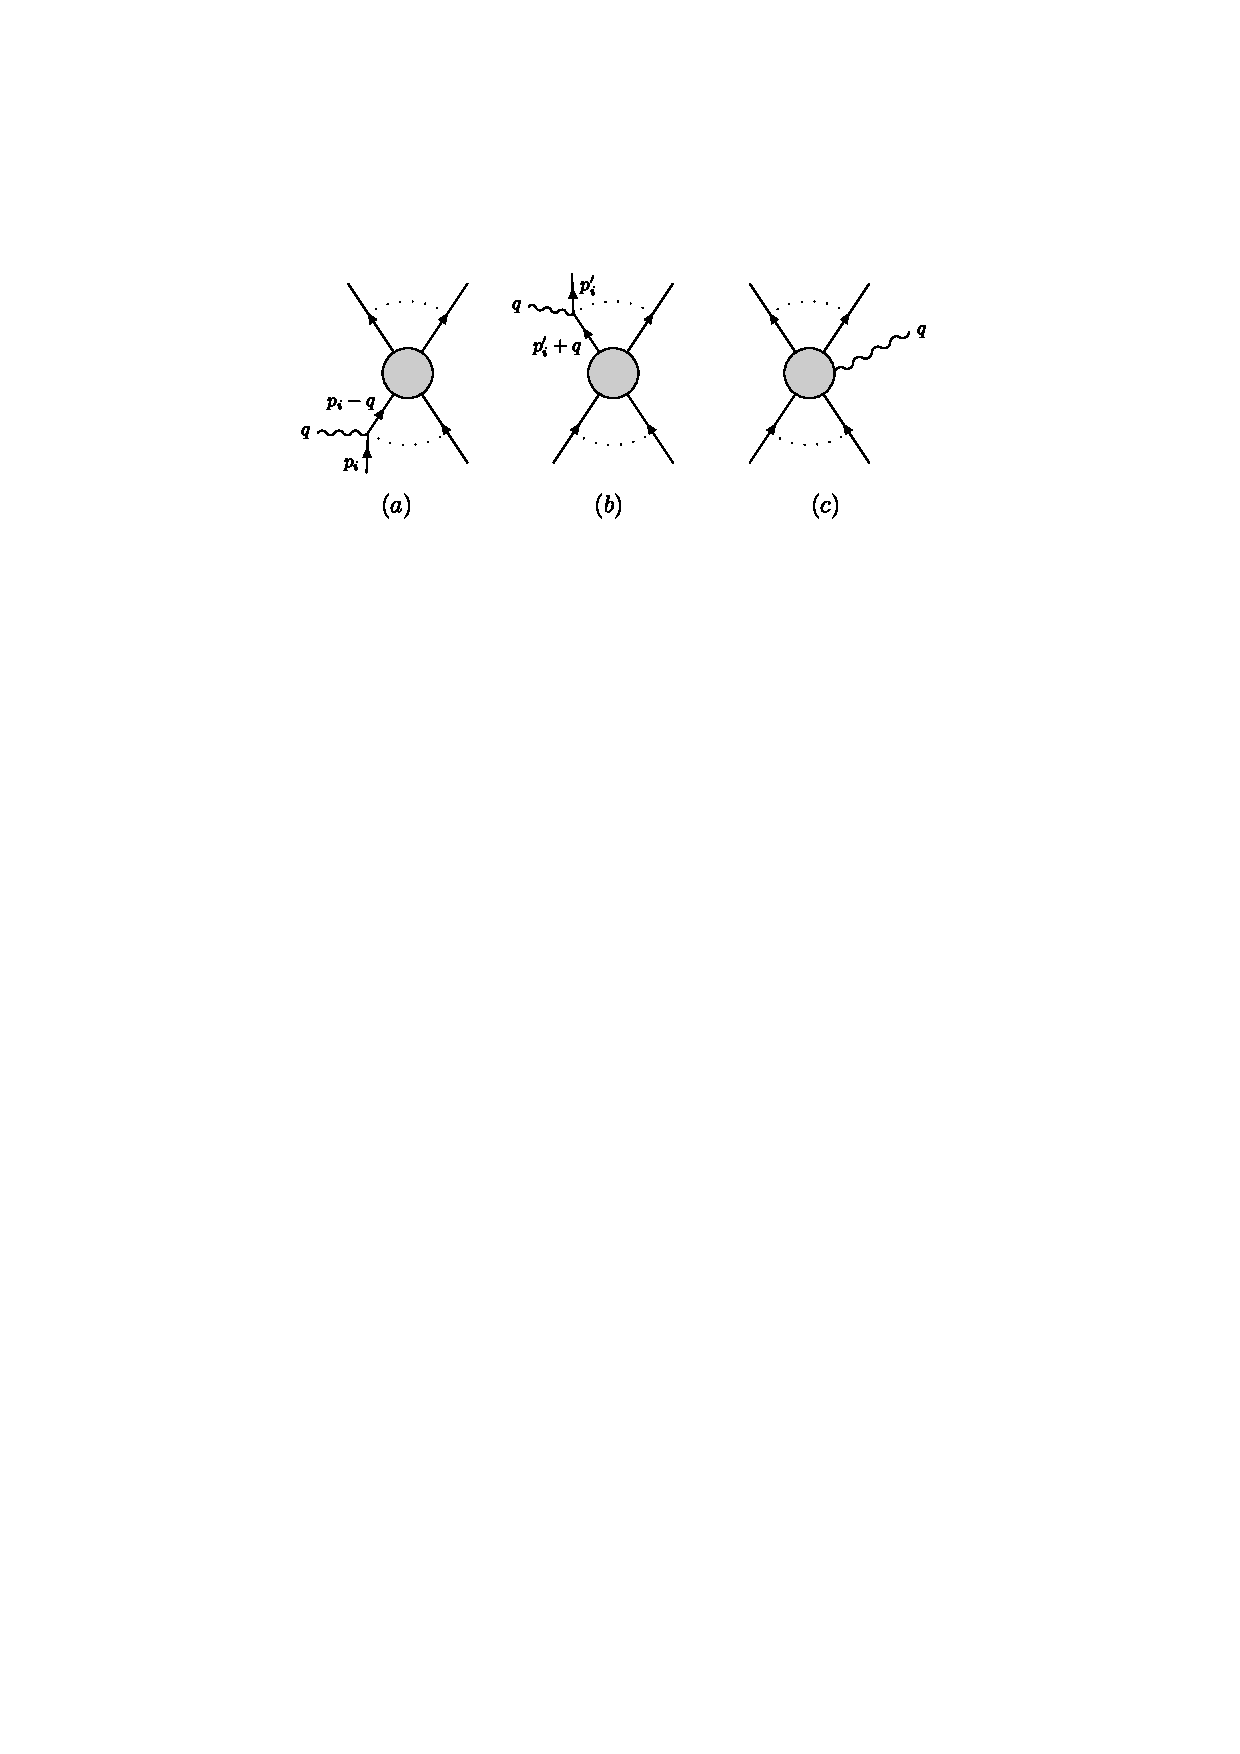
\includegraphics[width=0.8\linewidth]{figs/fig3.pdf}
	\caption{辐射软光子的三种情况}
\end{figure}
我们使用$\mathcal{A}(p,q)$表示辐射一个软光子后的振幅$\mathcal{A}(p)$表示没有辐射软光子的振幅(所有阶费曼图求和)。用$T(p_i-q)$表示原先没有辐射软光子的费曼图砍掉一个$p_i$外线但保留外线动量为非在壳的$p_i-q$得到的费曼图振幅,显然$T(p_i)u(p_i)=\mathcal{A}(p)$。

首先计算入射外线辐射软光子:
\begin{equation}
	\begin{aligned}
		Q_iT(p_i-q)\frac{(-\slashed{p}_i^\prime+\slashed{q}+m)\slashed{\epsilon}(q)}{(p_i-q)^2+m^2}u(p_i)&=-Q_iT(p_i-q)\Big[\frac{\epsilon(q)\cdot p_i+i\epsilon(q)_\mu q_\nu S^{\mu\nu}}{q\cdot p_i+\mathrm{i}0^+}\Big]u(p_i)
	\end{aligned}
\end{equation}
其中利用了$\slashed{a}\slashed{b}=-2a\cdot b-\slashed{b}\slashed{a}$,$q\cdot \epsilon_\pm(q)=0$以及狄拉克方程$(\slashed{p}+m)u(p)=0$。其中$S^{\mu\nu}=\frac{\mathrm{i}}{4}[\gamma^\mu,\gamma^\nu]$。唯一做近似的地方就是分母里面的$q^2$我们略去了,这对后面的高阶修正也不会影响。这一注意到$q=0$实际上是一个极点,这是因为在光子无线“软”的时候,多出来的那条内线传播子会无线趋于在壳,导致分母为0。

对于出射粒子辐射软光子也是类似的计算得到:
\begin{equation}\label{eq:20.17}
	\begin{aligned}
		Q^\prime_i\bar u(p_i^\prime)\frac{(-\slashed{p}_i^\prime-\slashed{q}+m)\slashed{\epsilon}(q)}{(p_i-q)^2+m^2}\bar T(p_i+q)&=Q^\prime_i\bar u(p_i^\prime)\Big[\frac{\epsilon(q)\cdot p_i+i\epsilon(q)_\mu q_\nu S^{\mu\nu}}{q\cdot p_i-\mathrm{i}0^+}\Big]\bar T(p_i-q)
	\end{aligned}
\end{equation}

至于内线发射光子,我们用$N^\mu(p,q)$表示,而且注意到$q\to0$时$N$非奇异,而且内线本身就是不在壳的,所以可以认为$N^\mu(p,q)\sim\mathcal{O}(q^0)$。三项加起来得到:
\begin{equation}\label{eq:21.3}
	\begin{aligned}
		\mathcal{A}(p,p^{\prime},q) =&\sum_\text{incoming }{ - Q _ i T ( p _ i - q )}\frac{\epsilon(q)\cdot p_i+i\epsilon(q)_{\mu}q_\nu S^{\mu\nu}}{q\cdot p_i+\mathrm{i}0^+}u(p_i)  \\
		&+\sum_{\mathrm{outgoing}}Q_{i}^{\prime}\bar{u}(p_{i}^{\prime})\frac{\epsilon(q)\cdot p_{i}^{\prime}+i\epsilon(q)_{\mu}q_{\nu}{S}^{\mu\nu}}{q\cdot p_{i}^{\prime}-\mathrm{i}0^+}\bar{T}(p_{i}^{\prime}+q)\\
		&+\epsilon(q)_{\mu}N^{\mu}(p,p^{\prime},q)
	\end{aligned}
\end{equation}
考虑最低阶修正,也就是只保留极点,得到:
\begin{equation}\label{eq:21.4}
	\boxed{
	\mathcal{A}(p,q)=\left[\sum_{i}\eta_iQ_{i}\frac{\epsilon(q)\cdot p_{i}}{q\cdot p_{i}}\right]\mathcal{A}(p)}+\mathcal{O}(1)
\end{equation}
其中对于入射粒子$\eta_i=-1$,出射粒子为$+1$。QED中辐射出光子的振幅都可以拆分成$\epsilon(q)_\mu \mathcal{M}^\mu$,振幅是相对论不变量,但是我们虽然常说$\epsilon(q)_\mu$是极化矢量,但它并不是真正意义上的矢量,因为其在lorentz变换下并不协变,而是会多出来一个正比于$q$的项\sn{我们是在Lorentz变换的意义下理解,其实矢量的这种变换完全可以理解为规范选取不同,从而从振幅的规范不变性导出结果。\cite{srednicki}}\cite{Weinberg}。为了让振幅是相对论不变量,必须有:
\begin{equation}\label{eq:21.5}
	\boxed{
	q_\mu\mathcal{M}^\mu=0}
\end{equation}
也就是Ward恒等式,也可以从Ward-高桥恒等式在U(1)对称性下导出它,实际上也就是利用电荷守恒导出它,但是前面我们的导出仅仅依赖于Lorentz不变性。现在把\ref{eq:21.4}中的$\epsilon(q)$替换为$q$我们得到:
\begin{equation}\label{eq:21.6}
	\left[\sum_i\eta_i Q_i\right]\mathcal{A}(p)=0
\end{equation}
也就是说,如果散射过程不被禁闭,也就是$\mathcal{A}(p)\neq 0$,那么这个过程必然要电荷守恒!另外说一句,我们这里的推导得到的\ref{eq:21.4}对于任意自旋的场都适用,比如对于标量QED,只需要把$S^{\mu\nu}$替换为0就好,不同的自旋对应$S^{\mu\nu}$的不同表示。

现在继续考虑两个光子的情况,两个光子由不同外线发射,在最低阶近似下只是乘上了\ref{eq:21.4}中两个因子,但是由相同外线发射就要考虑发射的先后顺序,因子形式会变化:
\begin{figure}[H]
	\centering
	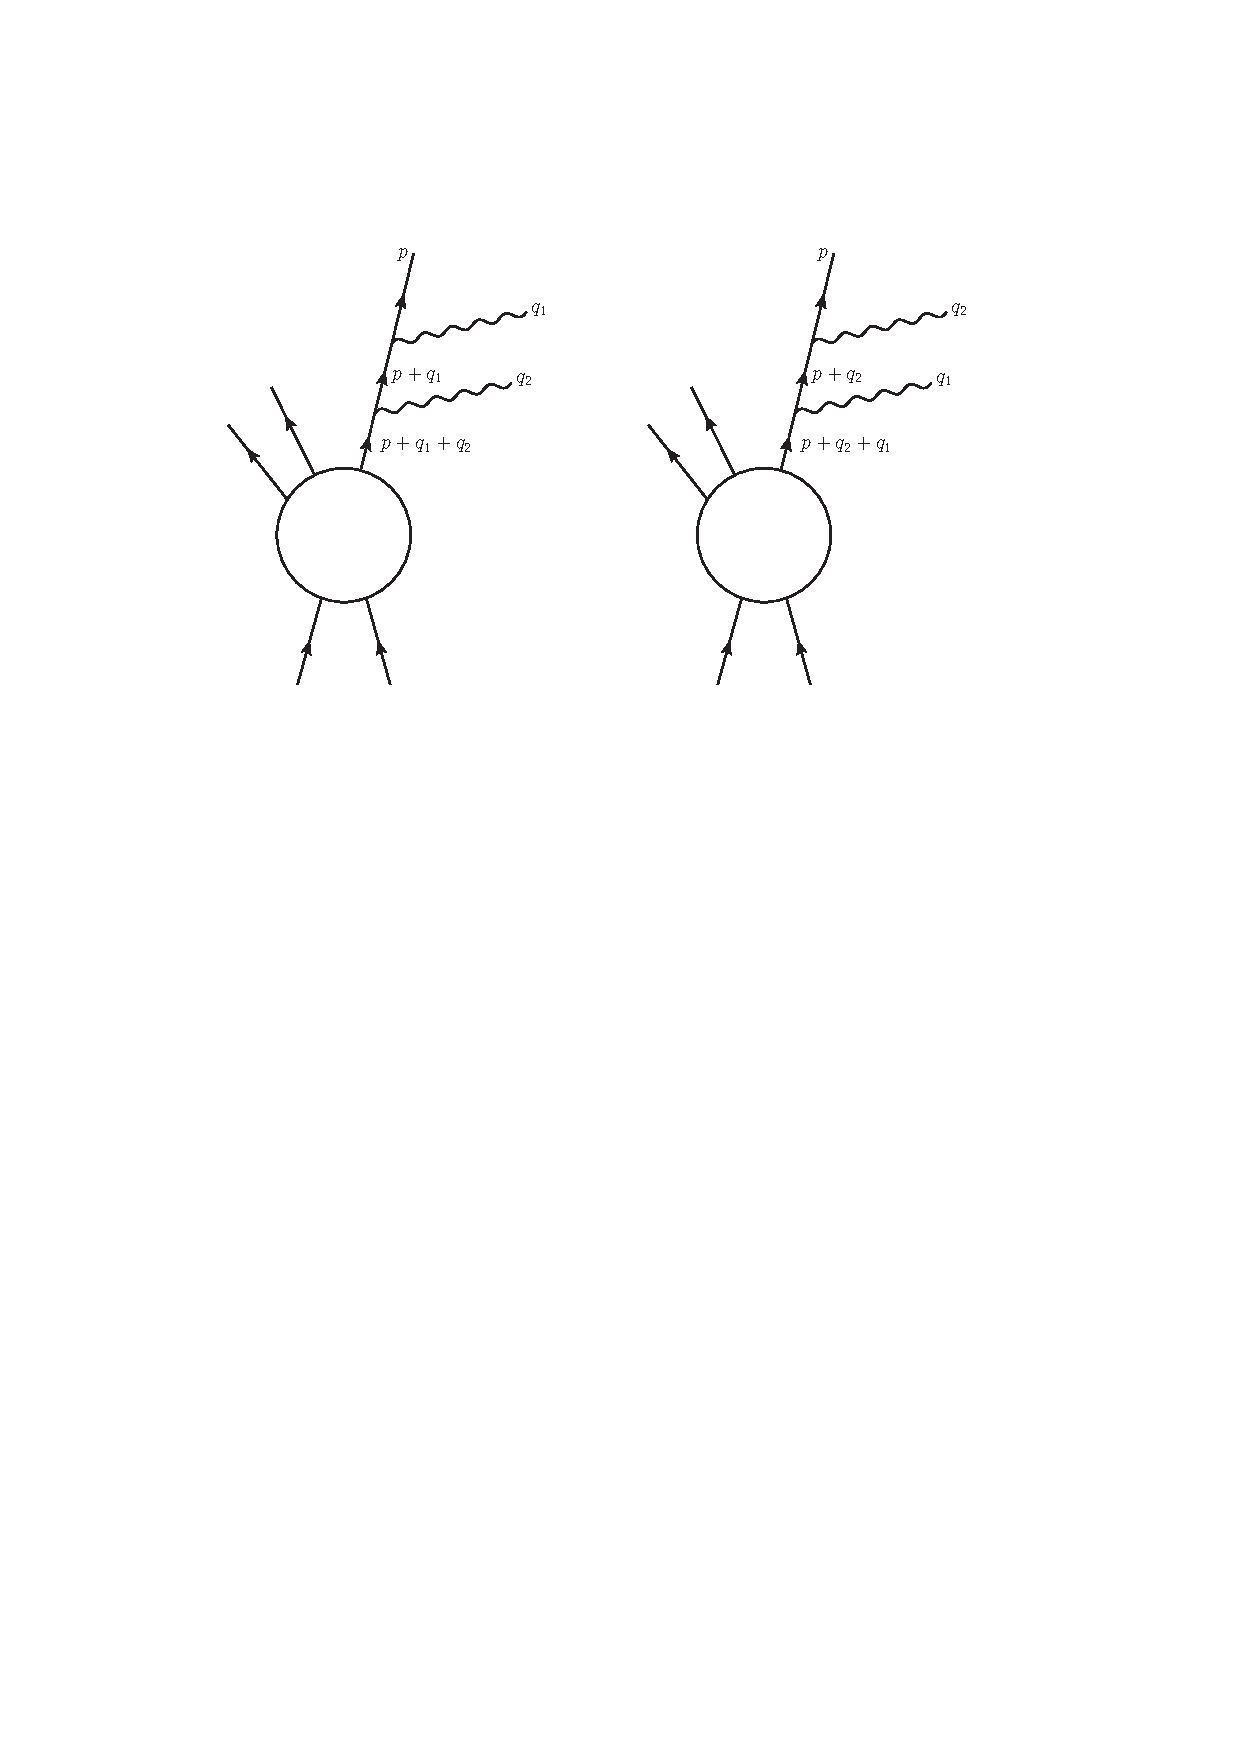
\includegraphics[width=0.8\linewidth]{figs/fig4.pdf}
	\caption{同一外线辐射两个软光子}
\end{figure}
把两幅图贡献的因子加起来得到:
\begin{equation}
	\begin{aligned}
	&\left[\frac{\eta Q\epsilon(q_1)\cdot p}{p\cdot q_1-\mathrm{i}\eta0^+}\right]\left[\frac{\eta Q\epsilon(q_2)\cdot p}{p\cdot(q_2+q_1)-\mathrm{i}\eta 0^+}\right]+\left[\frac{\eta Q\epsilon(q_2)\cdot p}{p\cdot q_2-\mathrm{i}\eta0^+}\right]\left[\frac{\eta Q\epsilon(q_1)\cdot p}{p\cdot(q_1+q_2)-\mathrm{i}\eta 0^+}\right]\\=&\left[\frac{\eta Q\epsilon(q_1)\cdot p}{p\cdot q_1-\mathrm{i}\eta0^+}\right]\left[\frac{\eta Q\epsilon(q_2)\cdot p}{p\cdot q_2-\mathrm{i}\eta 0^+}\right]	
	\end{aligned}
\end{equation}
得到的结果就是不同外腿上面的辐射两个软光子得到的因子,利用数学归纳法可以证明这一结论对于辐射任意数量的软光子都是适用的,那么最终我们只需要把因子乘起来,然后对所有外腿求和就好了,用式子表示如下:
\begin{equation}
	\boxed{\mathcal{A}(p,q_1,\ldots,q_m)=\prod_{j=1}^m\left[\sum_{i=1}^nQ_i\eta_i\frac{\epsilon(q_j)\cdot p_i}{q_j\cdot p_i}\right]\mathcal{A}(p)++\mathcal{O}(1)}
\end{equation}
前面的因子称为\textbf{eikonal因子}。推广到non-Abelian Y-M场的软定理也早有人计算过了\cite{Berends:1987me,Berends:1988zn,Mangano:1987kp,Mangano:1990by},软定理更多更一般的推广见\cite{McLoughlin:2022ljp}的文献索引。

现在来考虑辐射一个软引力子的情况,考虑第一节引入的标量场模型,传播子为:
\begin{equation}
	-\frac{i }{(p+\eta q)^2+m^2}
\end{equation}
顶点由\ref{eq:20.17}给出,但是由于\ref{eq:20.10},要与$\epsilon^{\mu\nu}$缩并,正比于$\eta_{\mu\nu}$的项没有贡献。以出射外线辐射软引力子为例,给出因子:
\begin{equation}
	i\sqrt{32\pi G}\varepsilon^{\mu\nu}p_{\mu}p_{\nu}\frac{-i}{\left(p+q\right)^{2}+m^{2}}\rightarrow\sqrt{8\pi G}\frac{\varepsilon^{\mu\nu}p_{\mu}p_{\nu}}{p\cdot q}
\end{equation}
求和后得到:
\begin{equation}
	\boxed{
	\mathcal{A}(p,q)=\left[\sum_i\frac{\kappa_i}{2}\eta_i\frac{\epsilon_{\mu\nu}(q)p_i^\mu p_i^\nu}{q\cdot p_i}\right]\mathcal{A}(p)+\mathcal{O}(1)}
\end{equation}

引力子同样有类似于\ref{eq:21.5}的恒等式,由此我们可以得到所有的$\kappa_i$都是相等的\sn{这里有点循环论证了,因为前面为了推导的方便我们同一取$\kappa_i=\sqrt{32\pi G}$},也就是等效原理!而自旋大于二的软粒子的软定理沿用上面的方法给出的限制就太强了,以至于散射$\mathcal{S}$矩阵必须trivial,所以一般认为自旋大于二的无质量粒子在“变软”的时候就脱耦合了。
\section{Subleading and subsubleading order soft theorem}
考虑动量为$\delta q,\delta \to0$的软光子辐射,$\pm$表示软光子的螺旋度,而$\ell_i$表示其它粒子的螺旋度,则更一般的软定理可以用洛朗展开写成:
\begin{equation}
	\mathcal{A}_{\ell_1,...,\ell_n,\pm}(p,\delta q)=\left[\sum_{a=0}^\infty\delta^{-1+a}S_\pm^{(a)}\right]\mathcal{A}_{\ell_1,...,\ell_n}(p)
\end{equation}
次领头阶的计算可以从\ref{eq:21.5}式出发,将\ref{eq:21.3}中所有的$\epsilon$替换为动量,保留到$\mathcal{O}(\delta^0)$,并且令等式左边为0。注意到这一阶近似下可以有$N^\mu(p,q)\approx N^\mu(p,0)$,得到:
\begin{equation}
	-q^{\mu}N_{\mu}(p,0)=\cancelto{0}{\frac{1}{\delta}\sum_{i=1}^{n}\eta_{i}Q_{i}\mathcal{A}(p)}+q^{\mu}\sum_{i=1}^{n}Q_{i}\frac{\partial}{\partial p_{i}^{\mu}}\mathcal{A}(p)
\end{equation}
其中第一项为0是因为电荷守恒\ref{eq:21.6},第二项中的$\partial_{p_i}$只作用于$\mathcal{A}$中的$T$,不作用于$u$\sn{因为这个式子的导出,是对$T(p\pm q)$展开得到的。}。这样就确定出了$N^\mu$\sn{其实只能确定到某个与$q$无关的矢量$v$,满足$q\cdot v=0$,但是这样的$v$实际上不存在。},再带回到\ref{eq:21.3}得到:
\begin{equation}
	A^\mu=\sum_{i=1}^nQ_i\left[\frac{\eta_ip_i^\mu}{\delta q\cdot p_i}+\frac{q^\nu p_i^\mu}{q\cdot p_i}\frac{\partial}{\partial p_i^\nu}-\frac{iq_\nu S_i^{\mu\nu}}{q\cdot p_i}-\frac{\partial}{\partial p_{i\mu}}\right]\mathcal{A}(p)+\mathcal{O}(\delta)
\end{equation}
这个式子里面的$\partial_{p_i}$就是作用于整个$\mathcal{A}$了。定义:
\begin{equation}
	L_i^{\mu\nu}=i\left(p_i^\mu\frac{\partial}{\partial p_{i\nu}}-p_i^\nu\frac{\partial}{\partial p_{i\mu}}\right),\quad J^{\mu\nu}_i+S_i^{\mu\nu}
\end{equation}
这里$S_i^{\mu\nu}$要根据第i个粒子的自旋去选取对应的Lorentz群不可约表示,比如$s=0,S^{\mu\nu}=0;s=\frac{1}{2},S^{\mu\nu}=\frac{i}{4}[\gamma^\mu,\gamma^\nu]$。这样我们就得到了包含subleading修正的软定理(LBK定理\cite{PhysRevLett.20.86,PhysRev.110.974}):
\begin{equation}
	\begin{aligned}S_{\pm}^{(0)}&=\sum_{i=1}^nQ_i\eta_i\frac{\epsilon_{\pm\mu}(q)p_i^\mu}{q\cdot p_i},\quad\text{and}\quad S_{\pm}^{(1)}&=-i\sum_{i=1}^nQ_i\frac{\epsilon_{\pm\mu}(q)q_\nu J_i^{\mu\nu}}{q\cdot p_i}\end{aligned}
\end{equation}
同样的方法可以推导出软引力子定理的subleading和subsubleading的修正项\sn{软定理已经使用不同的方法推了很多遍,文献\cite{McLoughlin:2022ljp,Brandhuber:2022qbk}中有不同证明方法的文献索引,而且还有对于更复杂的非阿贝尔规范理论的软定理讨论。}\cite{PhysRevD.90.084035,PhysRev.168.1623,White:2014qia,Broedel:2014fsa}:
\begin{equation}
	\begin{gathered}
		S_{\pm}^{(0)}=\frac{\kappa}{2}\sum_{i=1}^{n}\eta_{i}\frac{\epsilon_{\pm\mu\nu}(q)p_{i}^{\mu}p_{i}^{\nu}}{q\cdot p_{i}},\quad S_{\pm}^{(1)}=-i\frac{\kappa}{2}\sum_{i=1}^{n}\frac{\epsilon_{\pm\mu\nu}(q)p_{i}^{\mu}q_{\lambda}J_{i}^{\nu\lambda}}{q\cdot p_{i}}, \\
		S_{\pm}^{(2)}=-\frac{\kappa}{4}\sum_{i=1}^{n}\eta_{i}\frac{\epsilon_{\pm\mu\nu}(q)q_{\rho}q_{\sigma}J_{i}^{\mu\rho}J_{i}^{\nu\sigma}}{q\cdot p_{i}}
	\end{gathered}
\end{equation}

\section{Massless QED}
本章用天球的视角来看QED理论,为下一节做准备,本节的讨论都局限于比较简单的,不含磁荷而且电子没有质量的QED理论,但是基于此推出的许多结论实际上是普适的,可以推广到有质量QED上\cite{Strominger:2017zoo}。
\subsection{Classical}
弯曲时空中QED作用量:
\begin{equation}
	S_{EM}=-\frac{1}{2e^2}\int{F}\wedge\star F +S_M=-\frac{1}{4e^2}\int \mathrm{d}^4x\sqrt{-g}F_{\mu]nu}F^{\mu\nu}+S_M
\end{equation}
其中$S_M$由$j^\nu A_\nu$形式给出相互作用项,即$j^\nu=-\frac{\delta S_M}{\delta A^\nu}$。Maxwell场方程有下面简洁形式:
\begin{equation}
	\begin{cases}
		dF=0&\Rightarrow \nabla_\mu F_{\nu\rho}+\nabla_\nu F_{\rho\mu}+\nabla_\rho F_{\mu\nu}=0\\
		d\star F=e^2\star j&\Rightarrow \nabla_\mu F_{\mu\nu}=e^2j_\nu
	\end{cases}
\end{equation}
下式给出了整个空间内的净电荷/磁荷\sn{后文$\star,*$指的都是Hodge dual}:
\begin{equation}
	Q_E=\frac{1}{e^2}\int_{\mathcal{S}^2_\infty}\star F=\int_{\Sigma}\star j,\quad Q_M=\frac{1}{2\pi}\int_{\mathcal{S}^2_\infty} F
\end{equation}
它们是量子化的,只能取整数。QED是$U(1)$规范理论,在$A\mapsto A+d\varepsilon$的规范变换下理论不变,后文不加说明都在所谓\textbf{retarded radial 规范}下进行计算\cite{He:2014cra,Kapec:2015ena}:
\begin{equation}
	\begin{aligned}
		&\mathcal{I}^+: A_r=0,\quad A_u|_{\mathcal{I}^+}=0\\
		&\mathcal{I}^-: A_r=0,\quad A_v|_{\mathcal{I}^-}=0
	\end{aligned}
\end{equation}
在$\mathcal{I}^{\pm}$附近可以把$A,F$展开成$\mathcal{O}(1/r)$的形式,用$A^{(i)},F^{(i)}$表示$r^{-i}$项前的系数,那么在这一规范下有\sn{各项系数都只和$(u,z,\bar z)$相关了}:
\begin{equation}
	F_{ur}^{(0)}=A_u^{(0)}, F_{z\bar z}^{(0)}=\partial_z A_{\bar z}^{(0)}-\partial_{\bar z}A_z^{(0)},F_{uz}^{(0)}=\partial_u A_z^{(0)},F_{rz}^{(0)}=-A_z^{(1)}
\end{equation}
而且我们所关心的场位形在$\mathcal{I}^{+}_{+}$处为真空,即满足:
\begin{equation}
	\left.F_{ur}\right|_{\mathcal{I}_{+}^{+}}=\left.F_{uz}\right|_{\mathcal{I}_{+}^{+}}=0
\end{equation}
$\mathcal{I}^-$处类似。但这个规范选取就如库伦规范$\nabla\cdot \mathbf{A}=0$一样没有完全确定规范,$A^{(0)}_z$还可以进行下面的所谓Large gauge transformation:
\begin{equation}
	A^{(0)}_z\mapsto A^{(0)}_z+\partial_z\varepsilon(z,\bar z),\quad \forall \varepsilon\in C^\infty\left[C\mathcal{S}^2\right]
\end{equation}
规范变换是一种冗余,但是这里的Large gauge transformations 最大的特点就是在无穷远处不归零,这导致很多时候分部积分的边界项不能丢去,确确实实的成为了一个对称性,后面马上会看到会对应无穷多个守恒荷。

运动电荷激发的电磁场即所谓Li\'enard\mbox{-}Wiecher势\cite{Jackson1998ClassicalE3}。这里我们在天球坐标下将advanced和retarded势统一写为:
\begin{equation}
	F_{rt}(\vec{x},t)=\frac{e^2}{4\pi}\sum_{k=1}^n\frac{Q_k\gamma_k\left(r-t\hat{x}\cdot\vec{\beta}_k\right)}{\left|\gamma_k^2\left(t-r\hat{x}\cdot\vec{\beta}_k\right)^2-t^2+r^2\right|^{3/2}},\quad r^2=\vec{x}\cdot\vec{x},\quad\vec{x}=r\hat{x}
\end{equation}
其中我们假设所有电荷之间匀速运动,而且相互作用可忽略,这个假设有点强,但是请\textbf{相信}后面导出的结论是可以推广到一般情形的。现在计算在天球上的极限:
\begin{equation}
	\begin{aligned}
		&\left.F_{rt}\right|_{\mathcal{I}^{+}}=\frac{e^{2}}{4\pi r^{2}}\sum_{k=1}^{n}\frac{Q_{k}}{\gamma_{k}^{2}(1-\hat{x}\cdot\vec{\beta}_{k})^{2}}\\
		&\left.F_{rt}\right|_{\mathcal{I}^{-}}=\frac{e^{2}}{4\pi r^{2}}\sum_{k=1}^{n}\frac{Q_{k}}{\gamma_{k}^{2}(1+\hat{x}\cdot\vec{\beta_{k}})^{2}}
	\end{aligned}
\end{equation}
取极限,得到:
\begin{equation}
	\boxed{
	\left.F_{rt}\right|_{\mathcal{I}^{+}_-}\neq \left.F_{rt}\right|_{\mathcal{I}^{-}_+}}
\end{equation}
正是这个式子说明了要严格区分$\mathcal{I}^{+}_-,\mathcal{I}^{-}_{+}$和$i^0$。但是,因为$F_{ru}=F_{rt}=F_{rv}$:
\begin{equation}
	\boxed{
		\lim\limits_{r\to\infty}r^2F_{ru}(\hat{x})\Big|_{\mathcal{I}_{-}^+}=\lim\limits_{r\to\infty}r^2F_{rv}(-\hat{x})\Big|_{\mathcal{I}_{+}^-}
	}
\end{equation}
也就是说场在两个天球上是对径认同的,这也是为什么前面$\mathcal{I}^{\pm}$天球的角向选取是antipodal的,上边的式子可以写成下面很简洁的形式:
\begin{equation}
	\boxed{
	\left.F_{ru}^{(2)}(z,\bar z)\right|_{\mathcal{I}^{+}_-}=\left.F_{rv}^{(2)}(z,\bar z)\right|_{\mathcal{I}^{-}_+}
	}
\end{equation}
这个式子是普适的,而且非常重要,是后面散射问题的核心。现在考虑任意一个天球上的对径认同的函数:
\begin{equation}
	\varepsilon(z,\overline{z})|_{\mathcal{I}_{-}^{+}}=\varepsilon(z,\overline{z})|_{\mathcal{I}_{+}^{-}}
\end{equation}
定义下面的future charges和past charges:
\begin{equation}
	\boxed{
		Q_{\varepsilon}^{+}=\frac{1}{e^{2}}\int_{\mathcal I_{-}^{+}}\varepsilon*F,\quad Q_{\varepsilon}^{-}=\frac{1}{e^{2}}\int_{\mathcal I_{+}^{-}}\varepsilon*F
	}
\end{equation}
由于Hodge对偶后出来的体积元$\propto r^2$,所以在天球上$r\to\infty$,$F\to F^{(2)}$,再根据对径认同的条件,这样对于任意一个函数$\varepsilon$,我们都给出了一个“电荷”守恒律:
\begin{equation}
	\boxed{
	Q_\varepsilon^+=Q_\varepsilon^-
	}
\end{equation}
对于$\varepsilon$是常函数情形,就得到了一般的电荷守恒律。利用Stokes公式\sn{$\int_{\partial \Omega}\omega =\int_{ \Omega}d\omega$}可以改写$Q_\varepsilon^{\pm}$为\sn{$Q_\varepsilon^-$只用把$+\mapsto -$}:
\begin{equation}
	Q_\varepsilon^+=\frac{1}{e^2}\int_{\mathcal{I}^+}\mathrm{d}\varepsilon\wedge*F+\int_{\mathcal{I}^+}\varepsilon*j+\cancelto{0}{\frac{1}{e^2}\int_{\mathcal{I}_+^+}\varepsilon*F}
\end{equation}
最后一项为0是因为我们假设电子是无质量的,这样电子就是从$\mathcal{I}^-\to\mathcal{I}^+$,而不是$i^{-}\to i^+$,所以$F|_{\mathcal{I}_+^{+}}=0$。第一项是Soft term $Q_S^+$与软光子的产生湮灭有关,第二项由于是与流耦合,所以叫Hard term $Q_H^+$与带电实物粒子有关。将上面的微分形式写成分量形式\sn{其中使用了Bianchi恒等式:$\partial_{u}F_{ru}^{(2)}+D^{z}F_{uz}^{(0)}+D^{\bar{z}}F_{u\bar{z}}^{(0)}+e^2j_{u}^{(2)}=0$}:
\begin{equation}
	Q_{\varepsilon}^{+}=\underbrace{-\frac{1}{e^{2}}\int_{\mathcal{I}^{+}}dud^{2}z\left(\partial_{z}\varepsilon F_{u\bar{z}}^{(0)}+\partial_{\bar{z}}\varepsilon F_{uz}^{(0)}\right)}_{Q_{S}^{+}}+\underbrace{\int_{\mathcal{I}^{+}}dud^{2}z\varepsilon\gamma_{z\bar{z}}j_{u}^{(2)}}_{Q_{H}^{+}}
\end{equation}
定义Soft photon mode $N_z$:
\begin{equation}\label{eq:23.18}
	N_{z}\equiv \int_{-\infty}^{\infty}duF_{uz}^{(0)}=\lim_{\omega\to0}\int_{-\infty}^{\infty}duF_{uz}^{(0)}e^{i\omega u}
\end{equation}
再次看到$N_z$对应的是电磁场的零频部分,也就是软光子部分,而且有:
\begin{equation}
	\begin{aligned}
		\partial_{\bar{z}}N_{z}-\partial_{z}N_{\bar{z}}& =\int_{-\infty}^{\infty}du\left[\partial_{\bar{z}}F_{uz}^{(0)}-\partial_{z}F_{u\bar{z}}^{(0)}\right]  \\
		&=-\int_{-\infty}^{\infty}du\left.\partial_{u}F_{z\bar{z}}^{(0)}=-F_{z\bar{z}}^{(0)}\right|_{\mathcal{I}_{-}^{+}}^{\mathcal{I}_{+}^{+}}=0
	\end{aligned}
\end{equation}
最后等于0是因为$F_{z\bar z}|_{\mathcal{I}_{+}^{\pm}}=0$,本质上是因为没有磁单极子,磁场不是long-range的,在无穷远处为0\sn{因为$F_{z\bar z}=\frac{\partial x^{\mu}}{\partial z}\frac{\partial x^{\nu}}{\partial\bar{z}}F_{\mu\nu}=\frac{\partial x^{i}}{\partial z}\frac{\partial x^{j}}{\partial\bar{z}}F_{ij}$,而规范场强的空间分量$F_{ij}$只和磁场有关。}。所以$N_z$无旋,可以由此引申出一个实标量场$N$作为其原函数:
\begin{equation}
	N_z\equiv e^2\partial_zN=\int_{-\infty}^{\infty}duF_{uz}^{(0)}=A_{z}^{(0)}|_{\mathcal{I}_{+}^{+}}-A_{z}^{(0)}|_{\mathcal{I}_{-}^{+}}
\end{equation}
利用$N$,future charges可以写成下面简洁形式:
\begin{equation}\label{eq:23.21}
	Q_{\varepsilon}^{+}=2\int_{\mathcal{S}_\infty^2} d^{2}zN\partial_{z}\partial_{\bar{z}}\varepsilon+\int_{\mathcal I^{+}}dud^{2}z\varepsilon\gamma_{z\bar{z}}j_{u}^{(2)}
\end{equation}
对past charge也可以来上面的这一套:
\begin{equation}\label{eq:23.21.2}
	Q_{\varepsilon}^{-}=-2\int_{\mathcal{S}_\infty^2} d^{2}zN^-\partial_{z}\partial_{\bar{z}}\varepsilon+\int_{\mathcal I^{-}}dvd^{2}z\varepsilon\gamma_{z\bar{z}}j_{v}^{(2)}
\end{equation}
\subsection{Quantization}
上面讨论的都是经典场,现在进行量子化,目的是说明前面定义的future charge 和 past charges 都是 Large gauge transformations 对应的生成元算符。量子化方案选用正则量子化方案,这里使用的方法不需要事先对时空进行3+1分解,是协变的方法\cite{Ashtekar1987AsymptoticQ,Frolov:1979ab,1989thyg.book.....H,Lee:1990nz,Wald:1999wa}。

经典力学的正则形式是建立在辛几何上的,也就是给相流形上配备了一个非退化的、闭的二形式\cite{Arnold}:
\begin{equation}\label{eq:23.22}
	\Omega=\frac{1}{2}\omega_{IJ}dx^I\wedge dx^J
\end{equation}
而且可以证明,可以通过选取不同的广义坐标局部的将$\omega_{IJ}$化为下面的矩阵:
\begin{equation}
	\omega_{IJ}=\left.\left[\begin{matrix}0&1_{N\times N}\\-1_{N\times N}&0\end{matrix}\right.\right]
\end{equation}
力学量的Possion括号由下式给定:
\begin{equation}
	\{A,B\}=\Omega^{IJ}\partial_IA\partial_JB
\end{equation}
相空间是运动方程的解,可以与初始值一一对应。

到了场论这边,相空间我们可以选取为某一个柯西面$\Sigma$上的场位形。场$\phi$本身是流形上的微分形式,\ref{eq:21.22}中的$dx$应该替换为$\delta\phi$,这里$\delta$是场位形的在壳变分,也就是说$\phi+\delta \phi$仍然是场方程的解。场本身是定义在某个纤维丛上的,可以粗浅的理解为两个流形拼起来,而$d$是底流形上的微分形式算子,$\delta$事实上是另一个正交的微分形式算子,所以$\delta\phi$在$\delta$的意义上是1\mbox{-}form,在$d$的意义上$\delta$的作用不会改变其是几形式,这样$\Omega$形如$\delta\phi\wedge\delta\varphi$从$\delta$的意义上看就是个二形式。构建的微分形式还应当满足规范不变性,闭且非退化,而且还要对柯西面的不同选取一致,利用\cite{Wald:1999wa}中方法可以得到$U(1)$规范场的辛形式为:
\begin{equation}
	\Omega_{\Sigma}=-\frac{1}{e^{2}}\int_{\Sigma}\delta(*F)\wedge\delta A
\end{equation}
将柯西面选取为$\mathcal{I}^{\pm}$,得到分量为:
\begin{equation}
	\begin{aligned}
		\omega_{uz\bar{z}}|_{\mathcal{I}}+& =-\frac{1}{e^{2}}\left[\delta(*F)_{uz}\wedge\delta A_{\bar{z}}+\delta(*F)_{\bar{z}u}\wedge\delta A_{z}+\delta(*F)_{z\bar{z}}\wedge\delta A_{u}\right]_{\mathcal{I}^{+}}  \\
		&=-\frac{i}{e^{2}}\left[\delta F_{uz}^{(0)}\wedge\delta A_{\bar{z}}^{(0)}+\delta F_{u\bar{z}}^{(0)}\wedge\delta A_{z}^{(0)}\right],
	\end{aligned}
\end{equation}
其中利用了:\sn{注意到Levi-Civita符号不是张量,而是张量密度,$\sqrt{-g}\epsilon$才是张量,然后利用Hodge dual定义爆算即可}
\begin{equation}
	(*F)_{uz}=i\left(F_{uz}-F_{rz}\right),\quad(*F)_{z\bar{z}}=ir^{2}\gamma_{z\bar{z}}F_{ru}
\end{equation}
最终得到辛形式:
\begin{equation}\label{eq:23.29}
	\Omega_{\mathcal{I}^+}=\frac{1}{e^2}\int dud^2z\left[\delta F_{uz}^{(0)}\wedge\delta A_{\bar{z}}^{(0)}+\delta F_{u\bar{z}}^{(0)}\wedge\delta A_{z}^{(0)}\right]
\end{equation}
总是可以把$A_z$的$u\to\pm {\infty}$,也就是$\mathcal{I}^+_{\pm}$的与$u$无关的部分分离出去,这一部分又总是可以写成某个天球上标量场的导数,因为要求$F_{z\bar z}|_{\mathcal{I}_{+}^{\pm}}=0$:
\begin{equation}
	A_z^{(0)}(u,z,\bar{z})=\hat{A}_z(u,z,\bar{z})+\partial_z\phi(z,\bar{z}),\quad\partial_z\phi\equiv\frac{1}{2}\left[\left.A_z^{(0)}\right|_{\mathcal I_+^+}+\left.A_z^{(0)}\right|_{\mathcal I_-^+}\right]
\end{equation}
利用上面的分解以及soft photon mode重写\ref{eq:23.29}:
\begin{equation}
	\Omega_{\mathcal{I}^{+}}=\frac{2}{e^{2}}\int dud^{2}z\partial_{u}\delta\hat{A}_{z}\wedge\delta\hat{A}_{\bar{z}}-2\int d^{2}z\partial_{z}\delta\phi\wedge\partial_{\bar{z}}\delta N
\end{equation}
现在考虑正则量子化,场变成算符,而Poisson括号换成Dirac括号:\sn{$\{\quad,\quad\}\mapsto\frac{1}{i}[\quad,\quad]$}
\begin{equation}
	\begin{aligned}-\frac{2}{e^2}\left[\partial_u\hat A_z(u,z,\bar z),\hat A_{\bar w}(u',w,\bar w)\right]&=i\delta(u-u')\delta^2(z-w),\\2\left[\partial_z\phi(z,\bar z),\partial_{\bar w}N(w,\bar w)\right]&=i\delta^2(z-w).\end{aligned}
\end{equation}
积分得到:\sn{这里$$\Theta(u)=\frac{1}{\pi i}\int\frac{d\omega}{\omega}e^{i\omega u}=\begin{cases}+1&,u>0\\-1&,u<0\end{cases}$$}
\begin{equation}
	\begin{aligned}
		\left[\hat{A}_{z}(u,z,\bar{z}),\hat{A}_{\bar{w}}(u^{\prime},w,\bar{w})\right]& =-\frac{ie^{2}}{4}\Theta(u-u^{\prime})\delta^{2}(z-w),  \\
		[\phi(z,\bar{z}),N(w,\bar{w})]& =-\frac{i}{4\pi}\log|z-w|^{2}+f(z,\bar{z})+g(w,\bar{w}). 
	\end{aligned}
\end{equation}

\subsection{Large guage symmetry}
利用上面发展的对易式可以去计算$Q_\varepsilon^{\pm}$与场算符的对易关系,注意到物质场部分$Q_H$始终和规范场$A$对易,所以:
\begin{equation}
	\begin{aligned}&\left[Q_{\varepsilon}^{+},A_{z}^{(0)}(u,z,\bar{z})\right]=i\partial_{z}\varepsilon(z,\bar{z}),\\&\left[Q_{\varepsilon}^{-},A_{z}^{(0)}(v,z,\bar{z})\right]=i\partial_{z}\varepsilon(z,\bar{z}).\end{aligned}
\end{equation}
所以前面定义的守恒荷其实就是对径认同的Large gauge transformation的生成元,自然就是一个守恒荷!前面的讨论一直忽略了流耦合项$S_M$,加入后对前面的结论不会有影响,注意到$Q_S$与物质场对易,根据Noether定理:
\begin{equation}
	\left[j_{u}^{(2)}(u',w,\bar{w}),\Phi_{k}(u,z,\bar{z})\right]=-Q_{k}\Phi_{k}(u,z,\bar{z})\gamma^{z\bar{z}}\delta^{2}(z-w)\delta(u-u')
\end{equation}
这意味着:
\begin{equation}\label{23.36}
	\left[Q_\varepsilon^+,\Phi_k(u,z,\bar{z})\right]=\left[\int_{\mathcal{I}^+}\varepsilon*j,\Phi_k(u,z,\bar{z})\right]=-Q_k\varepsilon(z,\bar{z})\Phi_k(u,z,\bar{z})\equiv i\delta_\varepsilon\Phi_k(u,z,\bar{z})
\end{equation}
所以$Q_S$生成规范场的规范变换,$Q_H$生成费米场规范变换,合起来$Q_\varepsilon$生成$\mathcal{I}^+$上的local规范变换。
\section{Ward indentity = Soft theorem}
\subsection{Ward indentity of $\mathcal{S}$\mbox{-}Matrix}
量子力学里面就知道守恒意味着与哈密顿量对易,而$\mathcal{S}\sim \exp{iHT}$,所以前面的守恒荷会和$\mathcal{S}$对易:\sn{初末态基底选取平面波。}
\begin{equation}\label{eq:24.1}
	\boxed{\langle\mathrm{out}|\left(Q_\varepsilon^+\mathcal{S}-\mathcal{S}Q_\varepsilon^-\right)|\mathrm{in}\rangle=0}
\end{equation}
这样一个简单的式子就是$\mathcal{S}$\mbox{-}Matrix的Ward identity。利用\ref{eq:23.21}和\ref{eq:23.21.2}得到:
\begin{equation}
	\begin{aligned}
		Q_\varepsilon^-|\mathrm{in}\rangle&=-2\int d^2z\partial_{\bar{z}}\varepsilon\partial_zN^-(z,\bar{z})|\mathrm{in}\rangle+\sum_{k=1}^mQ_k^\mathrm{in}\varepsilon(z_k^\mathrm{in},\bar{z}_k^\mathrm{in})|\mathrm{in}\rangle \\
		\langle\mathrm{out}|Q_\varepsilon^+&=2\int d^2z\partial_z\partial_{\bar{z}}\varepsilon\langle\mathrm{out}|N(z,\bar{z})+\sum_{k=1}^nQ_k^\mathrm{out}\varepsilon(z_k^\mathrm{out},\bar{z}_k^\mathrm{out})\langle\mathrm{out}|
	\end{aligned}
\end{equation}
第一项没啥好说的,后面会讨论其物理含义,第二项的计算稍微提一下。首先我们假设入射态是$m$个hard particles,而且来自于天球上的点$z_k^{\mathrm{in}}$,\ref{23.36}给出了守恒荷与物质场之间的对易关系,实际上,不难证明守恒荷和产生湮灭算符也满足同样的对易关系\sn{比如标量场\cite{srednicki}$$a^{\dagger}(\mathbf{k})=-i\int d^{3}xe^{ikx}\stackrel{\leftrightarrow}{\partial_{0}}\varphi(x)$$}。以两个入射粒子为例:
\begin{equation}
	\begin{aligned}
		Q^-_{\varepsilon}\ket{\text{in}}&\sim Q^-_{\varepsilon}a_1^\dagger a_2^\dagger\ket{0}\\
		&\sim \left[Q^-_{\varepsilon},a_1^\dagger a_2^\dagger\right]\ket{0}+\cancelto{0}{a_1^\dagger a_2^\dagger Q^-_{\varepsilon}\ket{0}}\\
		&\sim  \left[Q^-_{\varepsilon},a_1^\dagger \right]a_2^\dagger\ket{0}+a_1^\dagger\left[Q^-_{\varepsilon},a_2^\dagger \right]\ket{0}\\
		&\sim Q_1\varepsilon_1\ket{\text{in}}+Q_2\varepsilon_2\ket{\text{in}}
	\end{aligned}
\end{equation}
第二行我们利用了真空态一定是没荷的。现在可以把\ref{eq:24.1}写为:
\begin{equation}
	\begin{aligned}
		2\int d^2z\partial_z\partial_{\bar{z}}\varepsilon\langle\text{out}|&\left(N(z,\bar{z})\mathcal{S}-\mathcal{S}N^-(z,\bar{z})\right)|\text{in}\rangle\\&=\left[\sum_{k=1}^mQ_k^\text{in}\varepsilon(z_k^\text{in},\bar{z}_k^\text{in})-\sum_{k=1}^nQ_k^\text{out}\varepsilon(z_k^\text{out},{\bar{z}}_k^\text{out})\right]\langle\text{out}|\mathcal{S}|\text{in}\rangle
	\end{aligned}
\end{equation}
取$\varepsilon(z,\bar z)=\frac{1}{w-z}$,则上式可以写为如下形式:\sn{$$\partial_{\bar{z}}\frac{1}{z-w}=2\pi\delta^2(z-w)$$}
\begin{equation}\label{eq:24.5}
	4\pi\langle\mathrm{out}|\left(\partial_zN\mathcal{S}-\mathcal{S}\partial_zN^-\right)|\mathrm{in}\rangle=\left[\sum_{k=1}^m\frac{Q_k^\mathrm{in}}{z-z_k^\mathrm{in}}-\sum_{k=1}^n\frac{Q_k^\mathrm{out}}{z-z_k^\mathrm{out}}\right]\langle\mathrm{out}|\mathcal{S}|\mathrm{in}\rangle 
\end{equation}
这个等式其实就是带有U(1) K$\breve{\text{a}}$c-Moody current的$\text{CFT}_2$的Ward恒等式\cite{Blumenhagen:2009zz,He:2015zea,Strominger:2013lka,Nande:2017dba}。
\subsection{Mode expansion}
本部分的终极目标是证明Ward恒等式可以联系渐近对称性和软定理,前文从相空间角度给出了Ward恒等式,在动量空间给出了软定理,是时候在动量空间重写Ward恒等式了,重点就是将场算符用平面波展开,也就是正则量子化的过程。free mode expansion 弯曲时空量子力学领域已经不少人算过了,U(1)规范理论结果如下:
\begin{equation}
	A_{\nu}(x)=e\sum_{\alpha=\pm}\int\frac{d^3q}{\left(2\pi\right)^3}\frac{1}{2\omega_q}\left[\varepsilon_{\nu}^{*\alpha}(\vec{q})a_{\alpha}^{\mathrm{out}}(\vec{q})e^{iq\cdot x}+\varepsilon_{\nu}^{\alpha}(\vec{q})a_{\alpha}^{\mathrm{out}}(\vec{q})^\dagger e^{-iq\cdot x}\right]
\end{equation}
$q$是平面波在壳动量$q^2=0$,$\varepsilon^\pm_\mu$是极化矢量,常常取为:
\begin{equation}\label{eq:24.7}
	\varepsilon^{+\mu}(\vec{q})=\frac1{\sqrt{2}}\left(\bar{z},1,-i,-\bar{z}\right),\quad\varepsilon^{-\mu}(\vec{q})=\frac1{\sqrt{2}}\left(z,1,i,-z\right),\quad q_{\mu}\varepsilon^{\pm\mu}(\vec{q})=0,\quad\varepsilon_{\alpha}^{\mu}\varepsilon_{\beta\mu}^{*}=\delta_{\alpha\beta}
\end{equation}
产生湮灭算符之间满足对易关系:
\begin{equation}
	\left[a_\alpha^{\mathrm{out}}(\vec q),a_\beta^{\mathrm{out}}(\vec q')^\dagger\right]=\delta_{\alpha\beta}(2\pi)^3(2\omega_q)\delta^3\left(\vec q-\vec q'\right)
\end{equation}
定义内积:
\begin{equation}
	(A,A')=-i\int d\Sigma^{\mu}[A^{\nu}(\nabla_{\mu}{A'}_{\nu}^{*}-\nabla_{\nu}{A'}_{\mu}^{*})-(A\leftrightarrow {A'}^{*})]
\end{equation}
这样定义的内积与类空超曲面$\Sigma$的选取是无关的。这样一来产生湮灭算符可以写成:
\begin{equation}
	a_\pm(q)=i({A},(\epsilon^\pm e^{iq\cdot x})^*)
\end{equation}
对于$\mathcal{I}^-$类似讨论,结果只是把out改成in。下面计算$A_z^{(0)}(u,z,\bar{z})\equiv\lim_{r\to\infty}A_z(u,r,z,\bar{z})$的模式展开:\sn{这里$\hat q,\hat x$都是指其空间部分}
\begin{equation}
	\begin{aligned}
		A_{\mu}(x) =&e\sum_{\alpha=\pm}\int\frac{d^3q}{\left(2\pi\right)^3}\frac{1}{2\omega_q}\left[\varepsilon_{\mu}^{*\alpha}(\vec{q})a_{\alpha}(\vec{q})e^{-i\omega_qu-i\omega_qr(1-\hat{q}\cdot\hat{x})}\right. \\
		&\left.+\varepsilon_{\mu}^{\alpha}(\vec{q})a_{\alpha}^{\dagger}(\vec{q})e^{i\omega_{q}u+i\omega_{q}r(1-\hat{q}\cdot\hat{x})} \right]\\
		=&\frac e{8\pi^2}\sum_{\alpha=\pm}\int_0^\infty d\omega_q\omega_q\int_0^\pi d\theta\sin\theta\left[\varepsilon_\mu^{*\alpha}(\vec{q})a_\alpha(\vec{q})e^{-i\omega_qu-i\omega_qr(1-\cos\theta)}\right. \\
		&\left.+\varepsilon_{\mu}^{\alpha}(\vec{q})a_{\alpha}^{\dagger}(\vec{q})e^{i\omega_{q}u+i\omega_{q}r(1-\cos\theta)}\right].
	\end{aligned}
\end{equation}
这里$\theta$是$\hat q$和$\hat x$之间的夹角,利用数学公式\sn{来源是鞍点近似}:
\begin{equation}
	\lim_{r\to\infty}\sin\theta e^{i\omega_qr(1-\cos\theta)}=\frac{i}{\omega_qr}\delta(\theta)+\mathcal{O}((r)^{-2})
\end{equation}
代入得到:
\begin{equation}
	A_\mu(x)=-\frac{ie}{8\pi^{2}r}\sum_{\alpha=\pm}\int_{0}^{\infty}d\omega_{q}\left[\varepsilon_{\mu}^{*\alpha}(\omega_{q}\hat{x})a_{\alpha}(\omega_{q}\hat{x})e^{-i\omega_{q}u}-c.c.\right]+\mathcal{O}(r^{-2})
\end{equation}
我们要求的玩意儿是$A_{z}=\partial_{z}x^{\mu}A_{\mu}$,注意到:
\[
	\partial_{z}x^{\mu}\varepsilon_{\mu}^{+}(\omega_{q}\hat{x})=0,\quad\partial_{z}x^{\mu}\varepsilon_{\mu}^{-}(\omega_{q}\hat{x})=\frac{\sqrt{2}r}{1+z\bar{z}}
\]
最终求得:\sn{下文中的$\omega$指$\omega_q$,即$q^0$}
\begin{equation}
	A_{z}^{(0)}(u,z,\bar{z})=-\frac{i}{8\pi^2}\frac{\sqrt{2}e}{1+z\bar{z}}\int_{0}^{\infty}d\omega\left[a_{+}^{\mathrm{out}}(\omega\hat{x})e^{-i\omega u}-a_{-}^{\mathrm{out}}(\omega\hat{x})^\dagger e^{i\omega u}\right]
\end{equation}
把定义式\ref{eq:28.18}改写为厄米的形式:
\begin{equation}
	\partial_zN=\dfrac{1}{2e^2}\lim_{\omega\to0^+}\int_{-\infty}^{\infty}du\left(e^{i\omega u}+e^{-i\omega u}\right)F_{uz}^{(0)}
\end{equation}
利用$A_z^{(0)}$重写上式为:
\begin{equation}
	\partial_zN=-\frac{1}{8\pi e}\frac{\sqrt{2}}{1+z\bar{z}}\lim_{\omega\to0^+}\left[\omega a_+^{\mathrm{out}}(\omega\hat{x})+\omega a_-^{\mathrm{out}}(\omega\hat{x})^\dagger\right]
\end{equation}
在$\mathcal{I}^-$上也有类似式子,只需要把$N\to N^-$,out$\to$in 就好。现在可以看出来为啥要叫soft photon mode 了。根据前面的铺垫,\ref{eq:24.5}终于可以写成如下形式:
\begin{equation}
	\begin{aligned}
		\operatorname*{lim}_{\omega\rightarrow0}\left\lfloor\omega\langle\mathrm{out}|\left(a_{+}^{\mathrm{out}}(\omega\hat{x})\mathcal{S}\right.\right.& \left.-\mathcal{S}a_{-}^{\mathrm{in}}(\omega\hat{x})^{\dagger}\right)|\mathrm{in}\rangle   \\
		&=\sqrt{2}e(1+z\bar{z})\left[\sum_{k=1}^{n}\frac{Q_{k}^\mathrm{out}}{z-z_{k}^\mathrm{out}}-\sum_{k=1}^{m}\frac{Q_{k}^\mathrm{in}}{z-z_{k}^\mathrm{in}}\right]\langle\mathrm{out}|\mathcal{S}|\mathrm{in}\rangle 
	\end{aligned}
\end{equation}
\subsection{Soft photon \& graviton}
前面用费曼图导出的软定理可以用$\mathcal{S}$矩阵写成如下形式:
\begin{equation}
	\lim\limits_{\omega\to0}\left[\omega\langle\text{out}|a_+^\text{out}(\vec{q})\mathcal{S}|\text{in}\rangle\right]=e\lim\limits_{\omega\to0}\left[\sum\limits_{k=1}^m\frac{\omega Q_k^\text{out}p_k^\text{out}\cdot\varepsilon^+}{p_k^\text{out}\cdot q}-\sum\limits_{k=1}^n\frac{\omega Q_k^\text{in}p_k^\text{in}\cdot\varepsilon^+}{p_k^\text{in}\cdot q}\right]\langle\text{out}|\mathcal{S}|\text{in}\rangle 
\end{equation}
这里出射和入射态都是平面波为基,而且我们把元电荷作为公因子提出,$Q\in\mathbb{Z}$,出入射动量用Embedding的形式写出来,前面第三部分写过,这里再写一遍:
\begin{equation}
	\begin{aligned}
		&q^{\mu} =\frac\omega{1+z\bar{z}}\left(1+z\bar{z},z+\bar{z},-i(z-\bar{z}),1-z\bar{z}\right),  \\
		&p_{k}^{\mu} =\frac{E_{k}}{1+z_{k}\bar{z}_{k}}\left(1+z_{k}\bar{z}_{k},z_{k}+\bar{z}_{k},-i(z_{k}-\bar{z}_{k}),1-z_{k}\bar{z}_{k}\right) 
	\end{aligned}
\end{equation}
注意到:
\begin{equation}
	\varepsilon_{+}^{\mu}(q)=\frac{1}{\sqrt{2}\omega}\partial_{z}\left[\left(1+z\bar{z}\right)q^{\mu}\right],\quad\varepsilon_{-}^{\mu}(q)=\frac{1}{\sqrt{2}\omega}\partial_{\bar{z}}\left[\left(1+z\bar{z}\right)q^{\mu}\right]
\end{equation}
带进去一通暴力计算,软定理被我们写成了:
\begin{equation}
\lim_{\omega\to0^+}\left[\omega\left\langle\mathrm{out}\right|a_+^\mathrm{out}(\omega\hat{x})\mathcal{S}\left|\mathrm{in}\right\rangle\right]\\=\frac{e}{\sqrt{2}}\left(1+z\bar{z}\right)\left[\sum_{k\in\mathrm{out}}\frac{Q_k}{z-z_k}-\sum_{k\in\mathrm{in}}\frac{Q_k}{z-z_k}\right]\left\langle\mathrm{out}\right|\mathcal{S}\left|\mathrm{in}\right\rangle
\end{equation}
根据${\mathcal{CPT}}$不变性:\sn{这里没搞懂为啥?}
\begin{equation}
\langle\text{out}|a_+^\text{out}(\vec{q})\mathcal{S}|\text{in}\rangle=-\langle\mathrm{out}|\mathcal{S}a_{-}^{\mathrm{in}\dagger}(\vec{q})|\mathrm{in}\rangle
\end{equation}
结合上面两个式子就证明了Ward恒等式和软定理是一回事,或者说通过Ward恒等式,软定理和 Large gauge symmetry 是一回事。这其实反过来说明了我们找到的 Large gauge symmetry 是non-trivial的,确实得看作是一个渐近对称性。这种non-trivial从记忆效应也能体现出来,后面会详细讨论。

回到引力这边,这边的证明思路上差不多,但是有很多比较微妙的点。首先就是守恒荷的量子化,虽然也可以按照QED那边的方法一样做,但是技术细节上微妙许多。不过我们可以猜测它们应当有如下形式:
\begin{equation}
	\boxed{
		\left[Q_f^+,\cdots\right]=i\delta f,\quad \left[Q_f^-,\cdots\right]=i\delta Y
	}
\end{equation}
至于$\delta_f$和$\delta_Y$的形式前面已经算过了,而且它们都是和哈密顿量对易的,这也是利用Ward恒等式的基础。第一个式子证明相对简单,可以看文献\cite{He:2014laa},第二个等式要复杂许多,首先是需要下面几个式子\cite{Ashtekar1987AsymptoticQ,Ashtekar:1978zz,Ashtekar:1981bq,PhysRevLett.46.573}:
\begin{equation}
	\begin{aligned}
		\begin{bmatrix}N_{\bar{z}\bar{z}}(u,z,\bar{z}),C_{ww}(u',w,\bar{w})\end{bmatrix}&=16\pi Gi\gamma_{z\bar{z}}\delta^2(z-w)\delta(u-u')\\
		\left[Q_{S}^{+},C_{zz}\right]&=-iuD_{z}^{3}Y^{z},\\\left[Q_{H}^{+},C_{zz}\right]&=\frac{iu}{2}D\cdot YN_{zz}+iY\cdot DC_{zz}-\frac{i}{2}D\cdot YC_{zz}+2iD_{z}Y^{z}C_{zz}
	\end{aligned}
\end{equation}
而且Superrotation对应的相空间也更加复杂\cite{Strominger:2016wns}。这些都只能先argue一下,细说太麻烦。同样也可以给出模式展开,这个时候$g^{\mu\nu}=\eta^{\mu\nu}+\kappa h^{\mu\nu}$,$h^{\mu\nu}$满足linearized Einstein equation:
\begin{equation}
	\partial_{\sigma}\partial_{\nu}h^{\sigma}{}_{\mu}+\partial_{\sigma}\partial_{\mu}h^{\sigma}{}_{\nu}-\partial_{\mu}\partial_{\nu}h-\Box h_{\mu\nu}=0
\end{equation}
Mode expansion为:
\begin{equation}
	{h}_{\mu\nu}(x)=\kappa\sum_{\alpha\in\pm}\int\frac{d^3k}{(2\pi)^3}\frac{1}{2k^0}\left[\epsilon_{\mu\nu}^{\alpha*}a_{\alpha}e^{ik\cdot x}+\epsilon_{\mu\nu}^{\alpha}a_{\alpha}^{\dagger}e^{-ik\cdot x}\right]
\end{equation}
若$h=0$,内积定义为:
\begin{equation}
	(h,h')=-i\int d\Sigma^\rho[h^{\mu\nu}(\nabla_\rho {h'}_{\mu\nu}^*-2\nabla_\mu {h'}_{\rho\nu}^*)-(h\leftrightarrow {h'}^*)]
\end{equation}
同样也可以用鞍点近似去求度规里的那些参数的模式展开,然后去证明软引力子定理,详细的计算移步至文献\cite{Kapec:2014opa,He:2014laa}。

\subsection{Asymptotic analysis on QED}
这一节的主要目的是讲一下历史进程,文献最早是通过类似于BMS的渐近分析得到守恒荷这些\cite{Strominger:2013lka,He:2014cra}。分析渐近对称性的第一步就是指定边界条件,从而找到允许的对称性。由于$T_{uu}$是能动张量$T_{00}$和$T_{0i}$的线性组合,所以它现在代表能流,由于天球半径按照$r^2$增大,所以为了让能量有限大,$T_{uu}\sim\mathcal{O}\left(\frac{1}{r^2}\right)$,根据Noether定理:
\begin{equation}
	T^{\mu\nu}=\frac{1}{16\pi}F^{\alpha\beta}F_{\alpha\beta}\eta^{\mu\nu}-\frac{1}{4\pi}F^{\mu\rho}\partial^{\nu}A_{\rho}
\end{equation}
进行对称化操作得到:\sn{这样子做最大的好处是现在不显含$A$,与规范无关了}
\begin{equation}
	T_{S}^{\mu\nu}\equiv T^{\mu\nu}-\frac{1}{4\pi}\partial_{\rho}\left(F^{\rho\mu}A^{\nu}\right)=\frac{1}{16\pi}F^{\alpha\beta}F_{\alpha\beta}\eta^{\mu\nu}-\frac{1}{4\pi}F^{\mu\rho}{F^{\nu}}_{\rho}
\end{equation}
改到Bondi坐标下:
\begin{equation}
	T_{uu}\sim F_{uz}F_{u\bar{z}}\frac{\gamma^{z\bar{z}}}{r^2}+\ldots 
\end{equation}
这个式子意味着$F_{uz}\sim\mathcal{O}(1)$,再根据$F_{ru},F_{rz}$是电磁场分量,所以渐近行为均为$\mathcal{O}(1/r^2)$。下面的一组$A$的渐近行为选取就满足这几个条件:\sn{这一节我们并不取定规范}\sn{这个条件充分但不必要,但是根据文献\cite{Campiglia:2016hvg,Conde:2016csj,Conde:2016rom}的讨论,选别的理论会变得不是很自然。}
\begin{equation}
	A_z\sim\mathcal{O}(1),\quad A_r\sim\mathcal{O}\left(\frac{1}{r^2}\right),\quad A_u\sim\mathcal{O}\left(\frac{1}{r}\right)
\end{equation}
而满足这一边界条件的规范变换只能是:
\begin{equation}
	\varepsilon=\varepsilon(z,\bar{z})+\mathcal{O}\left(\frac1r\right)
\end{equation}
无穷远(天球)处不归零,就是前面说的Large gauge transformations。类似于引力散射问题的分析,QED这边散射问题为了well-define,也必须把对径认同的要求看作是散射问题定义的一部分。
\section{Massive QED}

\section{Further Progress}
\subsection{Subleading order}
\subsection{Non-Abelian gauge theory}
\subsection{Higher dimensions}




	\part{A Crush Course on CFT}
% 计数器清零,每个part都要引用,除了part1
\setcounter{theorem}{0}
\setcounter{definition}{0}
\setcounter{lemma}{0}
\setcounter{sidenote}{1}

CFT经典教材是大黄书\cite{DiFrancesco:1997nk},教材\cite{Blumenhagen:2009zz,ito}也是不错的选择\sn{伊藤克司先生的书还没有官方中文译本,不过这里有民间译本的重排本\url{https://github.com/WHUZBF/CFT-book}},还有一些比较好的讲义\cite{Nawata:2022lsw,Ginsparg:1988ui,Qualls:2015qjb},共形场论的自举(bootstrap)方法也是非常重要的,可以见讲义\cite{Ribault:2014hia}的专门介绍。CFT也可以当作一门数学课来学习,偏重于数学的阅读材料有\cite{Schottenloher:2008zz}。

首先是一些Overview性质的介绍。CFT无非就是一种特殊的QFT,但是这个时候理论具有比Poincar\'e对称性更大的对称性,在二维的情况下甚至提升为无穷维的对称性,这种对称性能让我们不通过微扰场论直接确定关联函数。一般的QFT中我们用Poincar\'e的不同的不可约表示来标记不同的场,或者说,我们用自旋来标记场,到了CFT这边,我们还需要使用共形维数$\Delta$来标记,对于$s=0$的标量场,共形维数定义为在Dilation $x\mapsto\lambda x$ 下场变换为:
\begin{equation}
	\phi^\prime(\lambda \vec{x})=\lambda^{-\Delta}\phi(\vec x)
\end{equation}
但是这只是对Dilation要求场在共形变换下“协变”,进一步要求对任意共形变换“协变”就给出了\textbf{初级场}(primary field)的定义。\sn{注意我们遵从大黄书的符号约定,和\cite{Blumenhagen:2009zz,Ginsparg:1988ui}的定义恰巧相反,对最终CFT中的一些结论没有任何影响,仅仅只是中间推导过程有些细微的差别。}\sn{$s=1/2$是何形式?}
\begin{definition}
	共形维数为$\Delta$的初级场(s=0)定义为在任意共形变换下满足:
	\begin{equation}
		\phi^\prime(\vec{x^\prime})=\left|\frac{\partial \vec {x^\prime}}{\partial \vec {x}}\right|^{\Delta/d}\phi(\vec {x})
	\end{equation}
\end{definition}

初级场将是后面研究的主要对象。二维的共形对称性比较特殊,分为global和local的,如果上面的“协变性”只对global的共形变换适用,那我们称之为\textbf{准初级场}(quasi-primary field),显然初级场一定是准初级场,反过来却不一定。二维情况下我们还使用复平面为坐标\footnote{这是欧氏空间CFT的主要选取,也是后文研究的主要内容,Wick转动到闵氏时空之后选取所谓光锥坐标。},但是我们为了一些地方的方便,并不是考虑的$\mathbb{C}$,而是$\mathbb{C}^2$,也就是说我们把$z,\bar z$看作是完全独立的变量,进在一些特殊情况下认为$z^*=\bar z$。而且把$\Delta$拆分为共形权$(h,\bar h)=\frac{1}{2}\left(\Delta+s,\Delta-s\right)$在这一符号约定下,共形权定义变为:
\begin{equation}
	\boxed{
	\phi^{\prime}(\lambda z,\overline{\lambda}\overline{z})=\lambda^{-h}\overline{\lambda}^{-\overline{h}}\phi(z,\overline{z})
	}
\end{equation}
(准)初级场定义变为:
\begin{equation}
	\boxed{
		\phi^{\prime}\left(f(z),\overline{f}(\overline{z})\right)=\left(\frac{\partial f}{\partial z}\right)^{-h}\left(\frac{\partial\overline{f}}{\partial\bar{z}}\right)^{\overline{-h}}\phi(z,\bar{z})
	}
\end{equation}
如果$\phi$全纯我们称为\textbf{chiral},反全纯称为\textbf{anti-chiral}。无穷小共形变换$x\mapsto x+\epsilon$下:
\begin{equation}\label{ict}
	\boxed{
	\delta_{\epsilon,\bar{\epsilon}}\phi(z,\bar{z})\equiv\phi^\prime(x^\prime)-\phi(x)=-\left(h\partial_z\epsilon+\epsilon\partial_z+\overline{h}\partial_{\bar{z}}\bar{\epsilon}+\overline{\epsilon}\partial_{\bar{z}}\right)\phi(z,\overline{z})
	}
\end{equation}
\begin{remark}
	初级场的定义可以看作是一种拓宽的张量定义,考虑一个带$s$个协变指标的张量,在任意坐标变换$x\mapsto x+\epsilon(x)$下:
	\[-\delta\Phi_{\mu_1\cdots\mu_s}=\epsilon^\nu\partial_\nu\Phi_{\mu_1\cdots\mu_s}+(\partial_{\mu_1}\epsilon^\nu)\Phi_{\nu\mu_2\cdots\mu_s}+\cdots+(\partial_{\mu_s}\epsilon^\nu)\Phi_{\mu_1\cdots\mu_{s-1}\nu}\]
	换到复平面,简单起见只考虑全纯部分,那么$h=s$,上面的定义局限于$h$是整数,现在考虑任意取值,那些指标也没必要写出了,便得到:
	\[-\delta\Phi=\epsilon\partial\Phi+s\partial \epsilon\Phi\]
	这就是前面得到的无穷小变换形式。
\end{remark}

同QFT一样,这些场都会量子化成算符。不像QFT中我们研究的场是有限多个的,比如说QED就是正负电子对应的Dirac场和一个U(1)规范场耦合,CFT中我们研究的场很多情况下会是无穷多个的,因为我们把$\phi,\partial\phi$看作是不同的场,因为他们是不同共形权的初级场。定义一个CFT第一步就是告诉我们理论中有哪些初级场,也就是一个\textbf{谱}(Spectrum)$\{\mathcal{O}_{h,\bar h}\}$。CFT中我们并非按照微扰场论那一套来建立关联函数的计算方法的,而会去关注场之间的\textbf{算符乘积展开(OPE)},后面将会看到自举给出了OPE的绝大多数信息,还有一些系数是自举无法确定的,需要CFT的定义给定,这是定义CFT的第二个data。我们这样做是在算符的观点下看问题,或者说是在海森堡表象下看问题,那CFT的态是什么呢?这其实被所谓\textbf{态算符对应}联系起来。

最后想强调一点,正是因为CFT的思考方式和一般的QFT有比较大的不同,所以CFT的建立甚至是不需要已知理论的拉氏量的,我们需要知道的只是理论拥有的对称性,然后去找对称性的表示构造谱,能动量张量则刻画了CFT在共形变换下的性质,是构建OPE必须的,如果强行利用拉格朗日量进行分析反而会变得非常复杂,有的CFT甚至是没办法写下一个拉氏量的,但是通过自洽性分析我们是知道这种理论的存在性的,而且可以根据自举方法走得很远。

\section{Virasoro Algebra}
讨论共形场论,都是在量子层面上已经消去共形反常后的理论,比如YM理论就是量子化后存在共形反常的QFT,从而不能看作一个CFT。二维CFT的共形代数是$\mathrm{Witt}\times\overline{\mathrm{Witt}}$,后面我们讨论CFT其实都是在其中心扩张$\mathrm{Vir_c}\times\overline{\mathrm{Vir_c}}$下进行\sn{明确一下convention,扩张前的代数用小写$l$标记,扩张后的用大写$L$标记}。这里我不打算讨论过多中心荷的物理意义,这应当是弦论课的内容,为何要引入中心荷可以从群表示的观点来看。

首先如果一个CFT具有某个对称性,这个对称性构成了一个群,那么体系的谱就生活在这个群的群表示之中\sn{严格说是表示的最高权是那些初级场,也就是CFT的谱,由这些谱生成的次级态最终张成整个CFT的希尔伯特空间,也就是对称代数的表示。}。也就是说假设对称代数为$\mathfrak{V}\times\bar{\mathfrak{V}}$\sn{注意在二维CFT中我们都会将对称代数复化为两个独立的部分。两个独立的李代数可以作为线性空间考虑他们的直和$\mathfrak{V}\oplus\bar{\mathfrak{V}}$,这里写成$\times$也没错,是将他们考虑成集合,然后做卡氏积,由于两部分独立,所以这两者本质上没区别。},则:
\begin{equation}
	\boxed{\mathcal{S}=\bigoplus_{(\mathcal{R},\mathcal{R}^{\prime})\in\mathrm{Rep}(\mathfrak{V})^2}m_{\mathcal{R},\mathcal{R}^{\prime}}\mathcal{R}\otimes\bar{\mathcal{R}^{\prime}}}
\end{equation}
但是这个表示只需要是个射影表示就好,而射影表示对应的是李代数的中心扩张的表示。前面处理洛伦兹群我们不用考虑那么多,因为我们这证明了理论总是可以redefine来消去中心荷,但是一般的共形场论至少都有Virasoro对称性,而这个代数的中心荷是non-trivial的,一般是不能消除的,所以我们考虑对称性并非直接考虑$\mathrm{Vir}$,而是$\mathrm{Vir}_c$。
\begin{theorem}[Virasoro Algebra]
	\begin{equation}
		\boxed{
		\left[L_m,L_n\right]=\left(m-n\right)L_{m+n}+\frac c{12}\left(m^3-m\right)\delta_{m+n,0}
		}
	\end{equation}
\end{theorem}
\begin{remark}
	如果我们考虑$\mathfrak{sl}(2,\mathbbm{C})$子代数,会发现中心扩张是trivial的。
\end{remark}
\section{Radial Quantization and Hilbert Space}
\subsection{Radial Quantization}
对于$1+1$维时空,可以把空间方向一点紧化为圆,这样平面就会变为一个圆柱面,这样就可以引入圆柱面上的复坐标$w=x^0+ix^1$,这样$w\sim w+2\pi i$自动满足周期性条件,这也是弦论worldsheet的图像。而圆柱面又可以通过共形变换$w\mapsto e^w$变到另一个复平面上:
\begin{figure}[htbp]
	\centering
	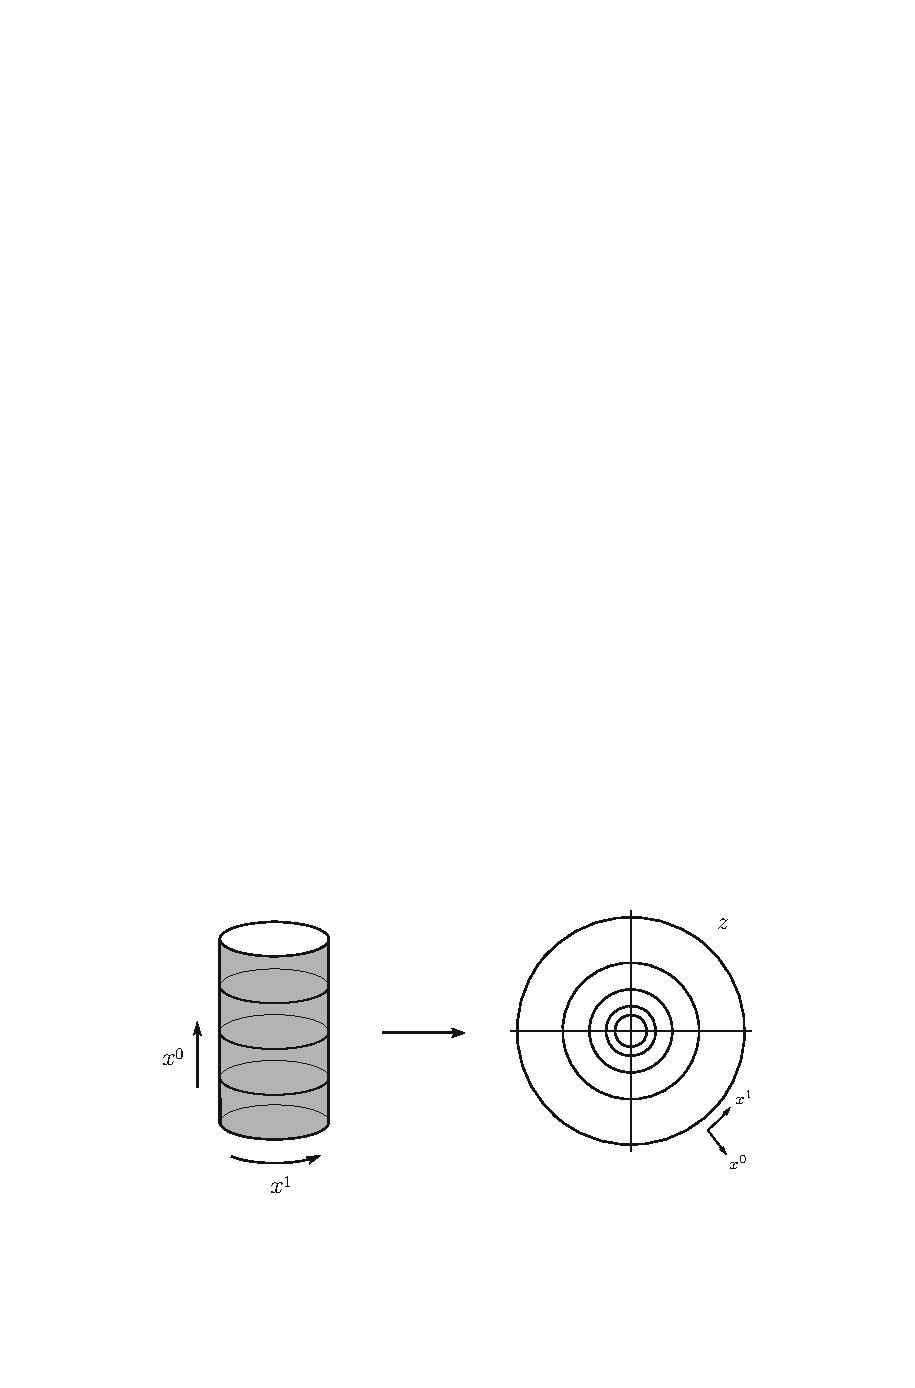
\includegraphics{figs/fig9.pdf}
	\caption{径向量子化}
\end{figure}
在这一变换下,时间方向变为了径向,空间方向变成了角向,而且把整个无穷远映射到了原点这一个点上。这下时间平移对应的哈密顿量$H$到复平面这边就变成了dilation算子$D$,而空间平移对应旋转$e^{i\theta}$:
\begin{equation}
		\boxed{H=L_0+\bar {L}_0,\quad P=i\left(=L_0-\bar {L}_0\right)}
\end{equation}
也正是因为时间方向变成了径向,时序积就应当变成“径向顺序积”,我们要去计算的就是径向顺序积的真空期望值,对于玻色子定义为:\sn{费米子把下面的情况改成负号就好}
\begin{equation}
	R\bigl(A(z)B(w)\bigr)\equiv\begin{cases}{}A(z)B(w)&\text{for }|z|>|w|,\\B(w)A(z)&\text{for }|w|>|z|.\end{cases}
\end{equation}

圆柱上的场我们用$\varphi(w,\bar w)$表示,复平面上的场用$\phi(z,\bar z)$表示,那么根据共形变换:
\begin{equation}
	\phi(z,\bar z)=z^{-h}{\bar {z}}^{-\bar h}\varphi(w,\bar w)
\end{equation}
在圆柱那边的CFT中我们知道$\varphi(w,\bar w)$可以做平面波展开为$e^{-ip^0x^0+ip^1x^1}$,由于我们考虑的是欧氏空间的场论,Wick转动后得到$e^{-p^0x^0+ip^1x^1}$,即$(e^{-w})^n(e^{-\bar w})^{\bar m}$的形式\sn{$n+m=p^0,n-m=p^1$}。而这恰恰就是洛朗展开的每一项!所以复平面上的CFT的模式展开为洛朗展开:
\begin{theorem}[Mode Expansion]
	\begin{equation}
		\boxed{\phi(z,\overline{z})=\sum_{n,\overline{m}\in\mathbb{Z}}z^{-n-h}\overline{z}^{-\overline{m}-\overline{h}}\phi_{n,\overline{m}}}
	\end{equation}
\end{theorem}
量子化场就是把$\phi_{n,\bar m}$量子化为算符,这些算符具有$(n,\bar m)$的权。

QFT微扰计算中一个非常重要的概念是渐近态,我们考虑的都是无穷远处的平面波入射经过复杂的相互作用后的平面波出射,微扰的角度看入射态就是在无穷远处的过去在真空附近施加一个扰动,也就是插入场算符,出射态也类似的这样做,这样就会自然出来时序积,然后LSZ约化这些的去计算振幅。同样的CFT这边也有这样的物理图景,只是现在无穷远处过去被映射到原点这一个点上了,所以渐近态应该定义为:
\begin{equation}
	ket{\phi}=\lim_{z,\overline{z}\to0}\phi(z,\overline{z})\ket{0}
\end{equation}
在原点处上式不奇异自然要求:\sn{这似乎告诉我们$n>-h,\bar m>-\bar h$对应的是CFT中的湮灭算符,后面讲到对易子会回到这里}
\begin{equation}\label{eq:30.6}
	\phi_{n,\overline{m}}\ket{0} =0\quad\text{for}\quad n>-h,\quad\overline{m}>-\overline{h}
\end{equation}
完整得到渐近态的公式:
\begin{equation}
	\boxed{|\phi\rangle=\lim\limits_{z,\overline{z}\to0}\phi(z,\overline{z})\left|0\right\rangle=\phi_{-h,-\overline{h}}\left|0\right\rangle}
\end{equation}
这里有个非常有趣的地方,本来一个算符里面有很多模,最后只剩下了一个,所以在CFT中,态和\textbf{局域}算符是唯一对应的!这就是态\mbox{-}算符对应。这和一般的QFT形成了鲜明的对比,那里一个场对应是不同“方向”平面波的组合,没有做到一一对应,但是CFT做到正是因为他把一个无穷大的空间部分在无穷远的过去全部紧化到了原点这一处,为了加深理解我们用路径积分的观点来看一下。

回忆量子力学中的传播子可以用路径积分表达为:
\begin{equation}
	G(x_f,x_i)=\int_{x(\tau_i)=x_i}^{x(\tau_f)=x_f}\mathcal{D}xe^{iS}
\end{equation}
那么演化后的末态波函数可以用初态波函数传播得到:
\begin{equation}
	\psi_{f}(x_{f},\tau_{f})=\int dx_{i}G(x_{f},x_{i})\psi_{i}(x_{i},\tau_{i})
\end{equation}
QFT这边“波函数”是一个泛函$\Psi[\phi(\sigma)]$,其模方表示在固定时间,空间中每个点$\sigma$上出现场构型$\phi(\sigma)$的概率,可以用路径积分得到末态:
\begin{equation}
	\Psi_f[\phi_f(\sigma),\tau_f]=\int\mathcal{D}\phi_i\int_{\phi(\tau_i)=\phi_i}^{\phi(\tau_f)=\phi_f}\mathcal{D}\phi e^{-S[\phi]}\Psi_i[\phi_i(\sigma),\tau_i]
\end{equation}
现在从柱面换到复平面CFT:
\begin{equation}
	\Psi_f[\phi_f(\sigma),r_f]=\int\mathcal{D}\phi_i\int_{\phi(r_i)=\phi_i}^{\phi(r_f)=\phi_f}\mathcal{D}\phi e^{-S[\phi]}\Psi_i[\phi_i(\sigma),r_i]
\end{equation}
不难发现初始态的作用是对$|z|=r_i$的积分进行加权,构造初始态需要在无穷远的过去,$r_i\to 0$,从而初始态只对原点处积分进行加权,等价于在原点处插入一个算子,即:
\begin{equation}
	\Psi[\phi_f;r]=\int^{\phi(r)=\phi_f}\mathcal{D}\phi e^{-S[\phi]}\mathcal{O}(z=0)
\end{equation}

\subsection{BPZ Conjugate}
为了构建关联函数,我们需要“左矢”,也就是厄米共轭来构造出射态从而有内积,这里谈的BPZ共轭是厄米共轭在Wick转动后的径向量子化欧氏空间CFT上的自然推广。不想扯过多物理上的考量,\cite{ito}从Wick转动后厄米共轭必须与时间反演一同定义BPZ共轭来解释了这一定义。
\begin{definition}[BPZ Conjugate]
	\begin{equation}
		\phi^\dagger(z,\overline{z})=\overline{z}^{-2h}z^{-2\overline{h}}\phi\left(\frac{1}{\overline{z}},\frac{1}{z}\right)
	\end{equation}
\end{definition}
另一方面直接从洛朗展开得到:
\begin{equation}
	\phi^{\dagger}(z,\overline{z})=\overline{z}^{-2h}z^{-2\overline{h}}\sum_{n,\overline{m}\in\mathbb{Z}}\overline{z}^{+n+h}z^{+\overline{m}+\overline{h}}\phi_{n,\overline{m}}=\sum_{n,\overline{m}\in\mathbb{Z}}\overline{z}^{+n-h}z^{+\overline{m}-\overline{h}}\phi_{n,\overline{m}}
\end{equation}
从而有:
\begin{equation}\label{BPZ}
	\boxed{
	\left(\phi_{n,\overline{m}}\right)^\dagger=\phi_{-n,-\overline{m}}
	}
\end{equation}
根据场的BPZ共轭定义,出射态应该定义为:
\begin{equation}
	\bra{\phi}=\lim\limits_{z,\overline{z}\to0}\bra{ 0  }              \phi^\dagger(z,\overline{z})=\lim\limits_{\overline{w},w\to\infty}w^{2h}\overline{w}^{2\overline{h}}\bra{0}\phi(w,\overline{w})=\bra{0}\phi_{h,\bar h}
\end{equation}
这里根据非奇异性要求了:
\begin{equation}\label{eq:30.17}
	\left<0\right|\phi_{n,\overline{m}}=0\quad\text{for}\quad n<h,\quad\overline{m}<\overline{h}
\end{equation}
当然,这里是根据定义严格来构造了一遍,实际计算疯狂使用\ref{BPZ}就好。
\section{Ward Identity and OPE}
\subsection{Infinitesimal Conformal Ward Identity}
前面$\S 4$已经看到共形对称性对应的守恒流可以使用$T_{\mu\nu}\epsilon^\nu$来构造,利用前面得到的最一般的Ward恒等式\ref{eq:19.11},对整个时空进行积分:
\begin{equation}
	\int dx^0dx^1\frac\partial{\partial x^{\mu}} \left\langle j_{a}^{\mu}(x)\Phi(x_{1})\cdots\Phi(x_{n})\right\rangle  =\sum_{i=1}^{n}\left<\Phi(x_{1})\delta_{\epsilon,\bar \epsilon}\cdots\Phi(x_{i})\cdots\Phi(x_{n})\right>
\end{equation}
$z=e^{x^0+ix^1}=x+iy$,进一步利用积分换元得到:\sn{别忘了雅可比行列式}
\begin{equation}
	\begin{aligned}
		\int dx^0dx^1&\partial_\mu\left\langle j_{a}^{\mu}(x)\Phi(x_{1})\cdots\Phi(x_{n})\right\rangle\\
		&=4\int dzd\bar z\left[\bar\partial(T_{\bar z\bar z}\epsilon)+\partial(T_{zz}\bar\epsilon)\right]\\
		&=2\int dxdy\left[\bar\partial(T_{\bar z\bar z}\epsilon)+\partial(T_{zz}\bar\epsilon)\right]
	\end{aligned}
\end{equation}
上面取了约定$\epsilon^z\equiv\epsilon(z),\partial_z\equiv\partial$,反全纯部分类似。现在考虑二元积分的格林公式:
\begin{equation}
	\begin{aligned}\oint_{\partial\Omega}P(x,y)dx+Q(x,y)dy=\int_\Omega dxdy\left(\frac{\partial Q}{\partial x}-\frac{\partial P}{\partial y}\right)\end{aligned}
\end{equation}
利用复变量$z=x+iy$可得下面的形式:\sn{就像是Wick转动一样,我们总假设这样随意复化是可行的}
\begin{equation}
	\begin{aligned}\oint_{\partial_\Omega}frac{1}{2}(P-iQ)dz+\frac{1}{2}(P+iQ)d\bar{z}=\int_\Omega dxdy(\partial(Q-iP)+\bar{\partial}(Q+iP))\end{aligned}
\end{equation}
上式中所有的围道积分都假设方向相对于$z$而言是逆时针,那么在$\bar z$平面上也就是逆时针,不过为了方便,而且CFT中我们也只考虑全纯部分,反全纯部分只要做个Conjugate就好了,后文中$\oint d\bar z$,表示围道方向相对于$\bar z$逆时针。
\begin{equation}
	\int_\Omega dxdy\left(\partial \bar f+\bar\partial f\right)=\frac{1}{2i}\oint_{\partial\omega}fdz+\bar f d\bar z
\end{equation}
再取:
\begin{equation}
	T(z)\equiv-2\pi iT_{zz},\bar T(\bar z)\equiv-2\pi iT_{\bar z\bar z}
\end{equation}
不过这个归一化因子并不重要,只是为了让OPE有一般的convention,后面比如自由玻色子这些具体模型我们都是先将归一化因子待定,再根据OPE的形式来确定它,只需要记住二维共形场论中$T_{zz}$始终全纯,$T_{\bar z\bar z}$始终反全纯就好了。归一化能动张量后,得到初级场的Ward恒等式:
\begin{equation}\label{ward}
	\boxed{
	\sum_{i=1}^{n}\left<\Phi(x_{1})\cdots\delta_{\epsilon,\bar \epsilon}\Phi(x_{i})\cdots\Phi(x_{n})\right>=\frac{1}{2\pi i}\oint\left\langle\left(T(z)\epsilon(z)dz+\bar T(\bar z)\bar \epsilon(\bar z)d\bar z\right)\Phi(x_{1})\cdots\Phi(x_{i})\cdots\Phi(x_{n})\right\rangle
	}
\end{equation}
这里积分围道包围所有$w_i$。根据上式我们可以定义\textbf{Conformal charge}:
\begin{equation}
	Q\equiv\frac{1}{2\pi i}\oint_{\mathcal{C}}\Bigl(dzT(z)\epsilon(z)+d\overline{z}\overline{T}(\overline{z})\overline{\epsilon}(\overline{z})\Bigr)
\end{equation}
这样便有:
\begin{equation}\label{eq:31.9}
	-\delta_{\epsilon,\bar\epsilon}\Phi=\left[Q,\Phi\right]
\end{equation}
\subsection{Operator Product Expansion}
但是\ref{eq:31.9}表面上有个非常大的漏洞,那就是因为全纯,直接导致围道积分始终为0。解决这一问题是注意到Q是一个算符,需要作用到其它场上面,而两个算符靠的非常近时真空涨落发散\sn{类似于$a_p,a_p^\dagger\sim\delta(0)$},上式积分中出现极点。也正是极点的存在导致我们定义局域算符之间的对易子的时候需要做正规化:
\begin{equation}
	[A(z,\bar{z}),B(w,\bar{w})]=\lim_{\begin{smallmatrix}|z|\rightarrow|w|\\|z|>|w|\end{smallmatrix}}A(z,\bar{z})B(w,\bar{w})-\lim_{\begin{smallmatrix}|z|\rightarrow|w|\\|w|>|z|\end{smallmatrix}}B(w,\bar{w})A(z,\bar{z})
\end{equation}
这直接导致对易子的计算可以等价于对径向顺序积的计算:\sn{后文中$\mathcal{C}(w)$表示只绕$w$的逆时针围道}
\begin{equation}
	\boxed{\begin{gathered}
			\oint dz\bigl[A(z),B(w)\bigr] =\oint_{|z|>|w|}dzA(z)B(w)-\oint_{|z|<|w|}dzB(w)A(z) \\
			=\oint_{\mathcal{C}(w)}dzR\Big(A(z)B(w)\Big), 
	\end{gathered}}
\end{equation}
现在利用只含一个初级场的无穷小变换Ward恒等式,或者说\ref{eq:31.9},注意到\ref{ict},以及:\sn{回忆$n$阶极点留数公式:\[\begin{aligned}
		\operatorname{Res}&[f(z),a]\\=&\lim\limits_{z\to a}\frac{1}{(n-1)!}\frac{d^{n-1}}{dz^{n-1}}\left[(z-a)^nf(z)\right]
	\end{aligned}\]}
\begin{equation}\label{eq:31.12}
	\begin{gathered}
		h\left(\partial_{w}\epsilon(w)\right)\phi(w,\overline{w}) =\frac{1}{2\pi i}\oint_{\mathcal{C}(w)}dzh\frac{\epsilon(z)}{(z-w)^{2}}\phi(w,\overline{w}), \\
		\epsilon(w)\left(\partial_{w}\phi(w,\overline{w})\right) =\frac1{2\pi i}\oint_{\mathcal{C}(w)}dz\frac{\epsilon(z)}{z-w}\partial_{w}\phi(w,\overline{w}).
	\end{gathered}
\end{equation}
得到全纯部分:
\begin{equation}
	R\left(T(z)\phi(w,\overline{w})\right)=\frac{h}{(z-w)^2}\phi(w,\overline{w})+\frac{1}{z-w}\partial_w\phi(w,\overline{w})+\ldots 
\end{equation}
\textbf{后面的省略号表示非奇异的项},大多数情况下我们要用的是OPE的奇异部分,因为它完全包含了和对易子一样的信息。像这样的把算符展开成其它算符和的形式称为\textbf{OPE}。在一般的QFT中我们计算时序积需要先写下路径积分,然后进行微扰展开算费曼图,但是CFT中我们只需要去考虑OPE就好了,对称性为我们简化了许多。后面写OPE会省略$R(\cdot)$,利用算符和能动张量之间的OPE我们还能给出一个初级场的等价定义:
\begin{theorem}
	一个场是共形权为$(h,\bar h)$的初级场\textbf{当且仅当}它满足:
	\begin{equation}\label{31.14}
		\boxed{\begin{gathered}
				T(z)\phi(w,\overline{w}) =\frac{h}{(z-w)^{2}}\phi(w,\overline{w})+\frac{1}{z-w}\partial_{w}\phi(w,\overline{w})+\ldots  \\
				\overline{T}(\overline{z})\phi(w,\overline{w}) =\frac{\overline{h}}{(\overline{z}-\overline{w})^{2}}\phi(w,\overline{w})+\frac{1}{\overline{z}-\overline{w}}\partial_{\overline{w}}\phi(w,\overline{w})+\ldots  
		\end{gathered}}
	\end{equation}
\end{theorem}
再次强调,之后写下的所有的OPE都应当认为是在在时序关联函数中插入算符时成立的关系!而且因为是时序积之中的关系:
\begin{equation}
	\langle\mathcal{O}_i(z,\bar{z})\mathcal{O}_j(w,\bar{w})\ldots\rangle=\sum_kC_{ij}^k(z-w,\bar{z}-\bar{w})\langle\mathcal{O}_k(w,\bar{w})\ldots\rangle 
\end{equation}
所以OPE结合律和交换律都自动满足。上式中$\ldots$表示其它任意算符的插入,当然既然是级数总有一个收敛半径,何时OPE的插入是有效的是我们需要关心的,从前面对OPE的推导可以看出我们要求积分围道中只有$w$这一个奇点,所以OPE是精确的当且仅当其它算符的插入点$\{w_i\}$满足$|w-w_i|>|z-w|$。

现在再回到Ward恒等式\ref{ward},但是现在考虑有多个$\Phi$的插入,从前面对OPE的分析得知围道内的极点是$\{w_i\}$,然后利用柯西定理将等式右边的积分换成对绕每个极点的围道积分求和得到:
\begin{equation}
	\begin{aligned}0=\oint\frac{dz}{2\pi i}\epsilon(z)&\Bigg[\Big\langle T(z)\phi_1(w_1,\overline{w}_1)\ldots\phi_N(w_N,\overline{w}_N)\Big\rangle\\
		&-\sum_{i=1}^N\left(\frac{h_i}{(z-w_i)^2}+\frac{1}{z-w_i}\partial_{w_i}\right)\Big\langle\phi_1(w_1,\overline{w}_1)\ldots\phi_N(w_N,\overline{w}_N)\Big\rangle\Bigg]\end{aligned}
\end{equation}
等式左边再次利用\ref{eq:31.12},得到所谓共形Ward恒等式(仅适用于初级场):\sn{注意这并不是代入$T,Phi$之间OPE得到的,因为前面说过OPE收敛半径等于与OPE处最近的其他算符插入处的距离。而我们下面要导出的等式与算符插入点完全无关,推导过程中看到我们将围道变形为单独绕每个$\{w_i\}$的围道来使得OPE的插入是精确的。}
\begin{equation}
	\boxed{\begin{aligned}\big\langle T\left(z\right)&\phi_{1}(w_{1},\overline{w}_{1})\ldots\phi_{N}(w_{N},\overline{w}_{N})\big\rangle\\&=\sum_{i=1}^{N}\left(\frac{h_{i}}{(z-w_{i})^{2}}+\frac{1}{z-w_{i}}\partial_{w_{i}}\right)\Big\langle\phi_{1}(w_{1},\overline{w}_{1})\ldots\phi_{N}(w_{N},\overline{w}_{N})\Big\rangle+\text{regular}\end{aligned}}
\end{equation}
\subsubsection{TT OPE}
CFT$_{2}$中非常重要的OPE是两个能动张量之间的OPE,就平面上的二维共形场论而言,chiral和anti-chiral部分是完全解耦的,所以:
\begin{equation}
	\boxed{
		T(z)\bar T(\bar w)=0
	}
\end{equation}
回忆能动张量$T\sim\frac{\delta S}\delta{g}$,现在来数质量量纲,由于$S$最终要放到指数上,所以$[S]=0$,再根据泛函导数定义$\frac{\delta f(x)}{\delta f(y)}=\delta^D(x-y)$,所以$[f]+\left[\frac{\delta }{\delta f}\right]=[\delta^D]=D$\sn{最后一个等号是因为$\int{dx^D}\delta^D(x-y)=1$,$[x]=-1$}。由于$[g]=0$,所以$[T]=2$,这暗示着在dilation下$T$的共形权为$(2,0)$,根据\ref{31.14}得到:
\begin{equation}
	T(z)T(w)=\cdots+\frac{2T(w)}{(z-w)^2}+\frac{\partial T(w)}{z-w}+\cdots
\end{equation}
第一个省略号是因为$T$不一定是初级场!第二个省略号表示奇异项。但是由于$[TT]=4$,所以最奇异的项只能是$(z-w)^{-4}$,而且分子只能是一个常数,我们取归一化为$c/2$得到:
\begin{theorem}[TT OPE]
	\begin{equation}\label{TT}
		\boxed{
			T(z)T(w)=\frac{c/2}{(z-w)^4}+\frac{2T(w)}{(z-w)^2}+\frac{\partial_wT(w)}{z-w}+\ldots 
		}
	\end{equation}
	$\bar T\bar T$的OPE取个conjugate就好。
\end{theorem}
有两点需要解释一下,首先是为何没有$(z-w)^{-3}$项的加入?这可以解释为由于OPE的交换律,所以$z\leftrightarrow w$对称性会紧闭所有奇数次数项。但是有一个例外是$(z-w)^{-1}$:
\begin{equation}
	\begin{aligned}T(w)T(z)&=\frac{c/2}{(z-w)^4}+\frac{2T(w)+2(z-w)\partial T(w)}{(z-w)^2}-\frac{\partial T(w)}{z-w}+\ldots=T(z)T(w)\end{aligned}
\end{equation}
可见$(z-w)^{-1}$的对称性被更低一阶项分子的泰勒展开保护,但是$(z-w)^{-3}$的更低一阶分子是常数,泰勒展开是trivial的。

虽然$T$并非初级场,但是是准初级场,因为$\{L_0,L_{\pm1}\}$的中心扩张是trivial的。虽然不是初级场,但是能动张量在$z\mapsto f(z)$的共形变换下的行为可以又下式描述:
\begin{theorem}
	\begin{equation}\label{schwarzian}
		\boxed{
			T^\prime(f(z))=\left(\frac{\partial f(z)}{\partial z}\right)^{-2}\begin{bmatrix}T(z)-\frac{c}{12}S(f(z),z)\end{bmatrix}
		}
	\end{equation}
	其中$S(f,z)$是Schwarzian导数,定义为:
	\begin{equation}
		\boxed{
			S(w,z)=\frac1{(\partial_zw)^2}\Big(\big(\partial_zw\big)\big(\partial_z^3w\big)-\frac32\big(\partial_z^2w\big)^2\big)
		}
	\end{equation}
\end{theorem}
观察一下无穷小共形变换下能动张量的性质:
\begin{equation}
	\begin{aligned}
		-\delta_{\epsilon}T(z)&=[Q,T]\begin{aligned}=\frac{1}{2\pi i}\oint_{\mathcal{C}(z)}dw\epsilon(w)T(w)T(z)\end{aligned}  \\
		&=\frac{1}{2\pi i}\oint_{\mathcal{C}(z)}dw\epsilon(w)\left(\frac{c/2}{(w-z)^{4}}+\frac{2T(z)}{(w-z)^{2}}+\frac{\partial_{z}T(z)}{w-z}+\ldots\right) \\
		&=\frac{c}{12}\partial_{z}^{3}\epsilon(z)+2T(z)\partial_{z}\epsilon(z)+\epsilon(z)\partial_{z}T(z).
	\end{aligned}
\end{equation}
不难证明在无穷小变换下\ref{schwarzian}的正确性。现在来考虑$T$模展开的对易子:
\begin{equation}
	T(z)=\sum_{n\in\mathbb{Z}}z^{-n-2}L_n\quad\text{where}\quad L_n=\frac{1}{2\pi i}\oint dzz^{n+1}T(z)
\end{equation}
\begin{proof}
	\begin{equation}
		\begin{aligned}
			\begin{bmatrix}L_{m},L_{n}\end{bmatrix}=&\oint\frac{dz}{2\pi i}\oint\frac{dw}{2\pi i}z^{m+1}w^{n+1}\bigl[T(z),T(w)\bigr]  \\
			=&\oint_{\mathcal{C}(0)}\frac{dw}{2\pi i}w^{n+1}\oint_{\mathcal{C}(w)}\frac{dz}{2\pi i}z^{m+1}R\Big(T(z)T(w)\Big) \\
			=&\oint_{\mathcal{C}(0)}\frac{dw}{2\pi i}w^{n+1}\oint_{\mathcal{C}(w)}\frac{dz}{2\pi i}z^{m+1}\bigg(\frac{c/2}{(z-w)^4}+\frac{2T(w)}{(z-w)^2}+\frac{\partial_wT(w)}{z-w}\bigg) \\
			=&\oint_{\mathcal{C}(0)}\frac{dw}{2\pi i}w^{n+1}\Big((m+1)m(m-1)w^{m-2}\frac c{2\cdot3!} \\
			&+2\left(m+1\right)w^m\left.T(w)+w^{m+1}\partial_wT(w)\right) \\
			=&\oint\frac{dw}{2\pi i}\left(\frac c{12}(m^3-m)\mid w^{m+n-1}\right. \\
			&\left.+2(m+1)w^{m+n+1}T(w)+w^{m+n+2}\partial_{w}T(w)\right) \\
			=&\frac c{12}\bigl(m^3-m\bigr)\delta_{m,-n}+2(m+1)L_{m+n} \\
			&+0-\underbrace{\oint\frac{dw}{2\pi i}(m+n+2)T(w)w^{m+n+1}}_{=(m+n+2)L_{m+n}}\\
			=&(m-n)~L_{m+n}+\frac c{12}\Big(m^3-m\Big)~\delta_{m,-n}
		\end{aligned}
	\end{equation}
	上面这一套是非常一般的做法。
\end{proof}
所以能动张量的Laurent模满足的是Virasoro代数。将这一套做法放到\ref{31.14}得到:
\begin{equation}\label{31.27}
	\boxed{\left[L_m,\phi_n\right]=\left((h-1)m-n\right)\phi_{m+n}}
\end{equation}
\subsection{n-point correlators (n<4)}
利用共形对称性实际上可以完全确定四点以下关联函数的形式。先来考虑准初级chiral场的关联函数,前面考虑的都是无穷小变换的Ward恒等式,但实际上在这里我们要使用的只是有限global共形变换的Ward恒等式,一般形式如下:
\begin{equation}\label{global ward}
	\boxed{
	\langle\phi_1'(x_1')\cdots\phi_N'(x_N')\rangle=\langle\phi_1(x_1')\cdots\phi_N(x_N')\rangle
	}
\end{equation}
上式等价于:
\begin{equation}
	\left\langle\phi_{1}\left(z_{1},\bar{z}_{1}\right)\cdots\phi_{n}\left(z_{n},\bar{z}_{n}\right)\right\rangle=\prod_{i=1}^{n}\left(\frac{\partial z'}{\partial z}\right)^{h_{i}}\left(\frac{\partial\bar{z}'}{\partial\bar{z}}\right)^{\bar{h}_{i}}\Bigg|_{z=z_{i},\bar{z}=\bar{z}_{i}}\left\langle\phi_{1}\left(z'_{1},\bar{z}'_{1}\right)\cdots\phi_{n}\left(z'_{n},\bar{z}'_{n}\right)\right\rangle 
\end{equation}
可以通过考察路径积分轻易得到。利用这一等式就可以得到一点关联函数必定是trivial的,这也可以根据前面的态算符对应要求的\ref{eq:30.6}\ref{eq:30.17}得到。
\begin{theorem}[2-pt]
	\begin{equation}\label{31.19}
		\left\langle\phi_i(z)\phi_j(w)\right\rangle=\frac{d_{ij}\delta_{h_i,h_j}}{(z-w)^{2h_i}}
	\end{equation}
\end{theorem}
\begin{theorem}[3-pt]
	\begin{equation}\label{31.20}
		\left\langle\phi_1(z_1)\phi_2(z_2)\phi_3(z_3)\right\rangle=\frac{C_{123}}{z_{12}^{h_1+h_2-h_3}z_{23}^{h_2+h_3-h_1}z_{13}^{h_1+h_3-h_2}}
	\end{equation}
	其中$z_{ij}\equiv z_i-z_j$
\end{theorem}
\begin{remark}
	$d_{\phi\phi},C_{123}$可以用关联函数写成下面的形式:
	\begin{equation}
		d_{\phi\phi}=\braket{\phi}{\phi}
	\end{equation}
	\begin{equation}
		C_{123}=\langle0|\phi_{(1)+h_1}\phi_{(2)h_3-h_1}\phi_{(3)-h_3}|0\rangle =\bra{\phi_1}\phi_{(2)h_3-h_1}\ket{\phi_3}
	\end{equation}
	这里$\phi_{(i)n}$表示$\phi_i$的第$n$个Laurent模。
\end{remark}
另外根据关联函数的单值性,还进一步要求\sn{后面考虑Virasoro代数表示的时候我们会先暂时忘掉这个要求。}\textbf{Chiral场的共形权只能是整数或者半整数}。把反全纯部分也加进来考虑得到:
\begin{itemize}
	\item 2-pt:
	\begin{equation}
		\left\langle\phi_1(z_1,\overline{z}_1)\phi_2(z_2,\overline{z}_2)\right\rangle=\frac{d_{12}}{z_{12}^{h_1+h_2}\overline{z}_{12}^{\overline{h}_1+\overline{h}_2}}\delta_{h_1,h_2}\delta_{\overline{h}_1,\overline{h}_2}
	\end{equation}
	\item 3-pt:
	\begin{equation}
		\begin{aligned}\big\langle\phi_1(z_1,\overline{z}_1)&\phi_2(z_2,\overline{z}_2)\phi_3(z_3,\overline{z}_3)\big\rangle\\&=\frac{C_{123}}{z_{12}^{h_1+h_2-h_3}z_{23}^{h_2+h_3-h_1}z_{13}^{h_1+h_3-h_2}\overline{z}_{12}^{\vec{h}_1+\vec{h}_2-\vec{h}_3}\overline{z}_{23}^{\vec{h}_2+\vec{h}_3-\vec{h}_1}\overline{z}_{13}^{\vec{h}_1+\vec{h}_3-\vec{h}_2} }\end{aligned}
	\end{equation}
\end{itemize}
根据OPE的交换性和结合性可以知道$C_{123}=C_{231}=C_{312}$。

关于这些公式的详细推导\cite{ito}上面都有,这里主要考虑用无穷小Ward恒等式的方法,但是我们考虑的毕竟是准初级场,所以只需要考虑$\epsilon(z)=\epsilon_{-1}+\epsilon_0z+\epsilon_1z^2$。将\ref{global ward}在无穷小变换下展开得到全纯部分:
\begin{equation}
	\boxed{
		\displaystyle\sum_{i=1}^{n}\left(h_{i}\partial_{i}\epsilon\left(z_{i}\right)+\epsilon\left(z_{i}\right)\partial_{i}\right)\left<\phi_{1}\left(z_{1}\right)\cdots\phi_{n}\left(z_{n}\right)\right>=0
	}
\end{equation}
这是一个微分方程,对于$\epsilon(z)=\epsilon_{-1}+\epsilon_0z+\epsilon_1z^2$恒成立,分开写可以写成:
\begin{equation}\label{31.37}
	\begin{aligned}\sum_i\partial_{w_i}\langle\phi_1(w_1)\cdots\phi_n(w_n)\rangle&=0\\\sum_i(w_i\partial_{w_i}+h_i)\langle\phi_1(w_1)\cdots\phi_n(w_n)\rangle&=0\\\sum_i(w_i^2\partial_{w_i}+2w_ih_i)\langle\phi_1(w_1)\cdots\phi_n(w_n)\rangle&=0\end{aligned}
\end{equation}
前面导出的Ward恒等式称为local的,现在这三个称为global的。所以我们可以通过求解这个微分方程来确定关联函数的形式,不难验证\ref{31.19}和\ref{31.20}就有这一特征。这种将关联函数计算转化为微分方程的求解的方法后面我们还会碰到。

但是四点及以上函数就不能确定到只差一个待定系数了,不过我们仍旧可以利用所谓\textbf{交叉对称性}(Crossing Symmetry)走的很远。

\subsection{General Form of the OPE}
为了简化讨论,先从chiral场开始,$\{\phi_i\}$表示CFT$_2$的Spectrum,下标$i$表示共形权为$h_i$,则OPE有下面的一般形式:
\begin{theorem}
	\begin{equation}
		\boxed{
		\phi_i(z)\phi_j(w)=\sum_{k,n\geq0}C_{ij}^k\frac{a_{ijk}^n}{n!}\frac{1}{(z-w)^{h_i+h_j-h_k-n}}\partial^n\phi_k(w)
		}
	\end{equation}
	其中:
	\begin{equation}\label{31.26}
		\begin{aligned}
			&a_{ijk}^{n} =\binom{2h_k+n-1}n^{-1}\binom{h_k+h_i-h_j+n-1}n,  \\
			&C_{ijk} =\sum_l{C_{ij}^{l}d_{lk}}
		\end{aligned}
	\end{equation}
\end{theorem}
由于1-pt关联函数始终为0,所以上面的OPE对两点关联函数的贡献只能是$n=0$且$h=0$的常值初级场贡献,也即$\left\langle\phi_1\phi_2\right\rangle\propto\frac{\delta_{h_1,h_2}}{z_{12}^{h_1+h_2}}$。
\begin{proof}
	考虑下面的关联函数:
	\begin{equation}
		\Big\langle\left(\phi_i(z)\phi_j(1)\right)\phi_k(0)\Big\rangle=\sum_{l,n\geq0}C_{ij}^l\frac{a_{ijl}^n}{n!}\frac{1}{(z-1)^{h_i+h_j-h_l-n}}\Big\langle\partial^n\phi_l(1)\phi_k(0)\Big\rangle 
	\end{equation}
	这里OPE的插入有效已经暗示$|z-1|<|0-1|=1$。利用两点关联函数的一般形式得到:
	\begin{equation}
		\left.\left\langle\partial_{z}^{n}\phi_{l}(z)\phi_{k}(0)\right\rangle\right|_{z=1}=\partial_{z}^{n}\left.\left(\frac{d_{lk}\delta_{h_{l},h_{k}}}{z^{2h_{k}}}\right)\right|_{z=1}=(-1)^{n}n!\left(\begin{matrix}2h_{k}+n-1\\n\end{matrix}\right)d_{lk}\delta_{h_{l},h_{k}}
	\end{equation}
	而3-pt关联函数的一般形式前面已经给出:
	\begin{equation}
			\Big\langle\left(\phi_i(z)\phi_j(1)\right)\phi_k(0)\Big\rangle=\frac{C_{ijk}}{(z-1)^{h_i+h_j-h_k}z^{h_i+h_k-h_j}}
	\end{equation}
	自洽性直接要求:
	\begin{equation}\label{31.30}
		\sum\limits_{l,n\geq0}C_{ij}^ld_{lk}a_{ijk}^n\binom{2h_k+n-1}{n}(-1)^n(z-1)^n\overset{!}{=}\frac{C_{ijk}}{\left(1+(z-1)\right)^{h_i+h_k-h_j}}
	\end{equation}
	由于$|z-1|<1$,所以可对右边利用下面的广义二项式定理进行展开:
	\begin{equation}
		\frac1{(1+x)^H}=\sum_{n=0}^\infty(-1)^n\binom{H+n-1}nx^n
	\end{equation}
	比较\ref{31.30}两边就得到了系数\ref{31.26},这其实就是Bootstrap的思想。
\end{proof}
Laurent模之间的一般对易关系形式为:
\begin{theorem}
	\begin{equation}
		\boxed{\left[\phi_{(i)m},\phi_{(j)n}\right]=\sum_kC_{ij}^kp_{ijk}(m,n)\phi_{(k)m+n}+d_{ij}\delta_{m,-n}\binom{m+h_i-1}{2h_i-1}}
	\end{equation}
	其中:
	\begin{equation}
		\begin{aligned}p_{ijk}(m,n)&=\sum_{\substack{r,s\in\mathbb{Z}_0^+\\r+s=h_i+h_j-h_{k-1}}}C_{r,s}^{ijk}\cdot\binom{-m+h_i-1}{r}\cdot\binom{-n+h_j-1}{s},\\C_{r,s}^{ijk}&=(-1)^r\frac{(2h_k-1)!}{(h_i+h_j+h_k-2)!}\prod_{t=0}^{s-1}(2h_i-2-r-t)\prod_{u=0}^{r-1}(2h_j-2-s-u)\end{aligned}
	\end{equation}
	这里$\mathbb{Z_0^+}$的意思是正整数以及0,后面的乘积$\prod$在$s=0(\text{or }r=0)$时定义为1,上面的系数形式还有一个非常重要的信息,就是只有当$h_k<h_i+h_j$时才有贡献。
\end{theorem}
通过共形对称性得到了OPE非常多的信息,唯一没有确定下来的只是一些系数,这就必须要CFT本身的一些性质了\sn{比如能动张量的形式,以及其它的对称性}。

更一般的非手征(准)初级场OPE的一般表达式更加复杂,形式为:
\begin{equation}
	\boxed{
		\phi_i(z,\overline{z})\phi_j(w,\overline{w})=\sum_{p}\sum_{\{k,\overline{k}\}}C_{ij}^p\frac{\beta_{ij}^{p,\{k\}}\overline{\beta}_{ij}^{p,\{\overline{k}\}}\phi_{p}^{\{k,\overline{k}\}}(w,\overline{w})}{(z-w)^{h_i+h_j-h_p-K}(\overline{z}-\overline{w})^{\overline{h}_i+\overline{h}_j-\overline{h}_p-\overline{K}}}
	}
\end{equation}
这里:
\begin{equation}
	\{\hat{L}_{-k_1}\ldots\hat{L}_{-k_n}\hat{\overline{L}}_{-k_1}\ldots\hat{\overline{L}}_{-k_n}\phi_p(z,\overline{z})\},\quad K\equiv\sum_i k_i
\end{equation}
$\beta_{ij}^{p,\{k\}}$和前面的$a^n_{ijk}$一样是之和初级场的共形权有关的,是与理论本身无关的可以计算出来的系数,我们唯一不知道的就是$C_{ij}^p$。
\subsubsection{Current Algebra}
\begin{definition}
	共形权为1的chiral(anti-chiral)场$j(z)$称为流。
\end{definition}
考虑一个谱为$N$个流的理论,根据前面Laurent模的一般形式得到:
\begin{equation}\label{current}
	\begin{bmatrix}j_{(i)m},j_{(j)n}\end{bmatrix}=\sum_kC_{ij}^kp_{111}(m,n)j_{(k)m+n}+d_{ij}m\delta_{m,-n}
\end{equation}
$d_{ij}$在$i\neq j$时为0,但是不同的$ij$对应的比例系数不同。我们总是可以通过rescal这些流,使得$d_{ij}=k\delta_{i,j}$,然后再通过对流进行重新组合得到:
\begin{equation}
	\boxed{
		\begin{bmatrix}j_m^i,j_n^j\end{bmatrix}=i\sum_lf^{ijl}j_{m+n}^l+km\delta^{ij}\delta_{m,-n}
	}
\end{equation}
这些流的模构成了一个Lie代数,显然中心荷non-trivial,后面会进一步详细讨论。它实际上是仿射化之后得到的{\itshape Ka\v{c}-Moody}代数。
\section{Crossing Symmetry}
本节的目的是最大程度得到四点关联函数$\langle\phi_1(z_1,\bar{z}_1)\phi_2(z_2,\bar{z}_2)\phi_3(z_3,\bar{z}_3)\phi_4(z_4,\bar{z}_4)\rangle $的信息。$n<4$的可以完全确定从数学上看是因为黎曼球面上任意两个或三个点,都可以通过共形变换映射为固定的$\{0,1,\infty\}$,但是四点我们最多只能将他们映射到$\{0,x,1,\infty\}$,其中$x$是\textbf{交比(Crossing Ratio)}。
\begin{equation}
	x=\frac{(z_1-z_2)(z_3-z_4)}{(z_1-z_3)(z_2-z_4)},\quad\bar{x}=\frac{(\bar{z}_1-\bar{z}_2)(\bar{z}_3-\bar{z}_4)}{(\bar{z}_1-\bar{z}_3)(\bar{z}_2-\bar{z}_4)}
\end{equation}
所以四点关联函数用前面的方法只能确定到一个与交比有关的函数。利用\ref{global ward},我们知道任意四点关联函数可以与下面的关联函数联系起来:\sn{$z\mapsto \frac{(z_1-z)(z_3-z_4)}{(z-z_4)(z_1-z_3)}$}
\begin{equation}
	\propto \langle\phi_i(0,0)\phi_j(x,\bar x)\phi_l(1,1)\phi_m(\infty,\infty)\rangle\equiv G^{ij}_{lm}(x,\bar x)
\end{equation}
由于OPE由结合律,所以可以前两个先做OPE,后两个在做OPE,注意到$\braket{\phi_p}{\phi_q}\sim\delta_{h_p,h_q}$,我们可以将上式重写为:
\begin{equation}\label{32.3}
	G^{ij}_{lm}(x,\bar x)=\sum_pC_{ij}^pC_{lm}^p\mathcal{F}_{ij}^{lm}(p\mid x)\overline{\mathcal{F}}_{ij}^{lm}(p\mid\overline{x})
\end{equation}
这里的$\mathcal{F}_{ij}^{lm}(p\mid x)$称为\textbf{Conformal Block},关联函数就是由这些Block线性组合而来的。再次利用\ref{global ward},考虑$z\mapsto 1-z$和$z\mapsto 1/z$,有:
\begin{equation}
	G^{ij}_{lm}(x,\bar x)=\langle\phi_i(1,1)\phi_j(1-x,1-\bar x)\phi_l(0,0)\phi_m(\infty,\infty)\rangle= G^{lj}_{im}(1-x,1-\bar x)
\end{equation}
\begin{equation}
	G^{ij}_{lm}(x,\bar x)=x^{2h_j}\bar x^{2\bar h_j}\langle\phi_i(1,1)\phi_j(\frac{1}{x},\frac{1}{\bar x})\phi_l(\infty,\infty)\phi_m(0,0)\rangle= x^{2h_j}\bar x^{2\bar h_j}G^{mj}_{il}(\frac{1}{x},\frac{1}{\bar x})
\end{equation}
这让我们得到另外两个$G(x,\bar x)$的表达式:
\begin{align}
	\label{32.6} G(x,\bar x)&=\sum_pC_{im}^pC_{jl}^p\mathcal{F}_{im}^{jl}(p\mid1-x)\overline{\mathcal{F}}_{im}^{jl}(p\mid1-\overline{x})\\
	\label{32.7} G\left(x,\bar x\right)&=x^{-2h_j}\overline{x}^{-2\overline{h}_j}\sum_pC_{il}^pC_{jm}^p\mathcal{F}_{il}^{jm}\left(p\mid\frac1x\right)\overline{\mathcal{F}}_{il}^{jm}\left(p\mid\frac1{\overline{x}}\right)
\end{align}
这三个等式对应不同顺序的OPE缩并,就像是QFT中费曼图的$s,t,u$三个channel,$p$就像是中间的传播子,共形不变性要求这三个$G(x,\bar x)$的等式殊途同归,这就给出了$C^p_{ij}$必须要满足的一套等式,共形自举的思想就是通过这套方程完全确定OPE系数。
\begin{figure}[htbp]
	\centering
	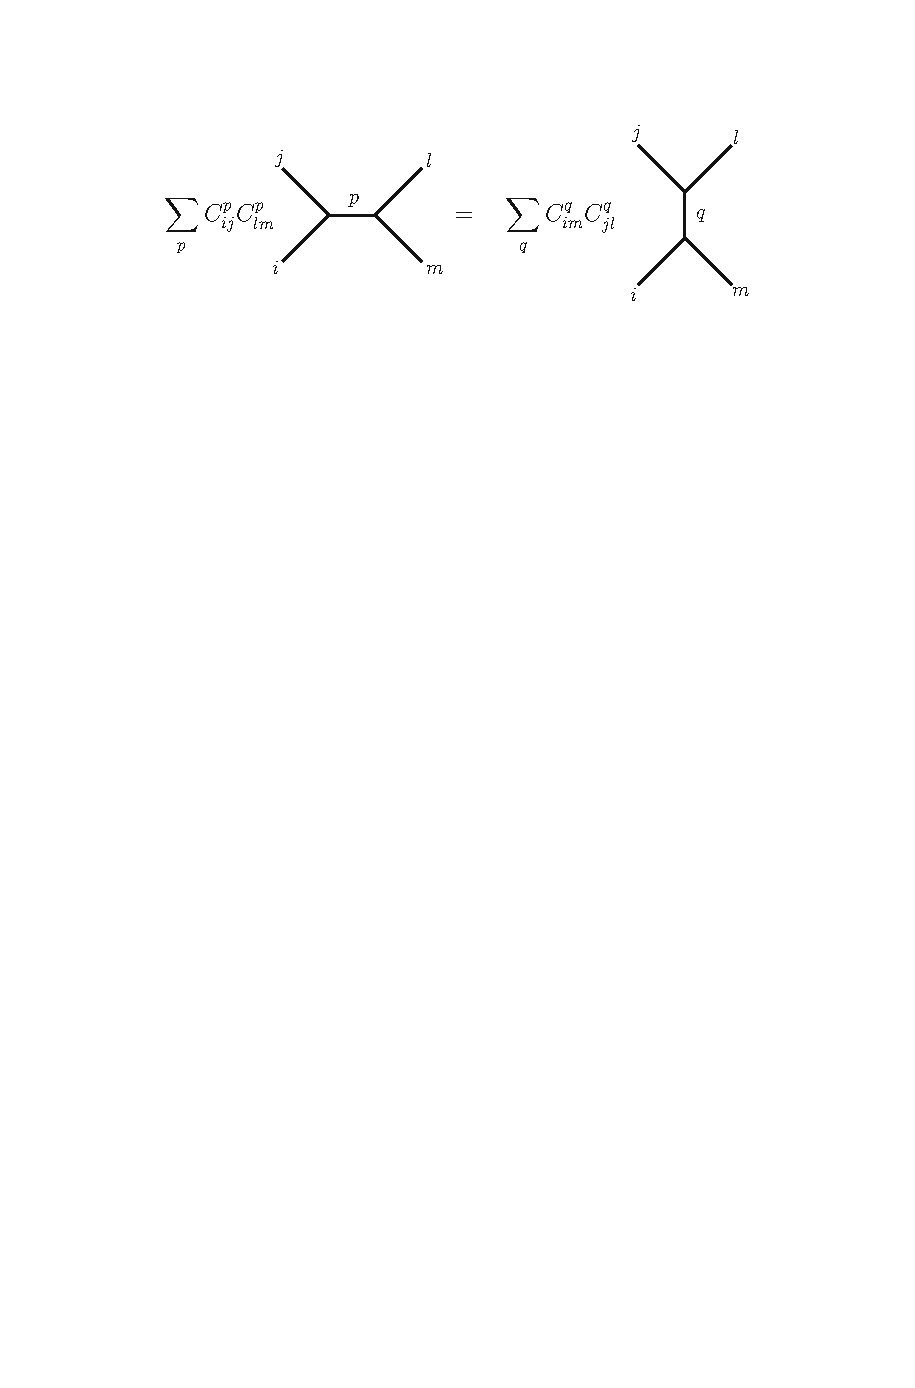
\includegraphics{figs/fig10.pdf}
	\caption{$G(x)=G(1-x)$ Crossing Symmetry的图示}
\end{figure}
\subsection{Fusing and Braiding Matrices}
考虑一个比较简单的情形,CFT的谱是个有限谱\sn{比如RCFT},这样Conformal Blocks构成了一个有限维线性空间,其中的某个线性组合得到的元素就是我们要的四点关联函数\sn{当然还要把全纯反全纯组合起来}。这其实就是在说\ref{32.3},\ref{32.6}和\ref{32.7}中的Conformal Blocks相差的仅仅是一个线性变换,他们是同一个线性空间的不同基底!
\begin{equation}
	\mathcal{F}_{ij}^{kl}(p\mid x)=\sum_qB{\left[\begin{smallmatrix}j&k\\i&l\end{smallmatrix}\right]}_{p,q}\mathcal{F}_{ik}^{jl}\!\left(q\mid\frac1x\right)
\end{equation}
\begin{equation}
	\mathcal{F}_{ij}^{kl}(p\mid x)=\sum_qF{\left[\begin{array}{cc}j&k\\i&l\end{array}\right]}_{p,q}\mathcal{F}_{il}^{jk}(q\mid1-x)
\end{equation}
这里$B$称作\textbf{Braiding Matrices},$F$称作\textbf{Fusing Materices},$p,q$是标记矩阵元,$\{i,j,l,m\}$标记矩阵本身。我们用类似轮换序图的形式来表达上面的两个方程:
\begin{figure}[H]
	\centering
	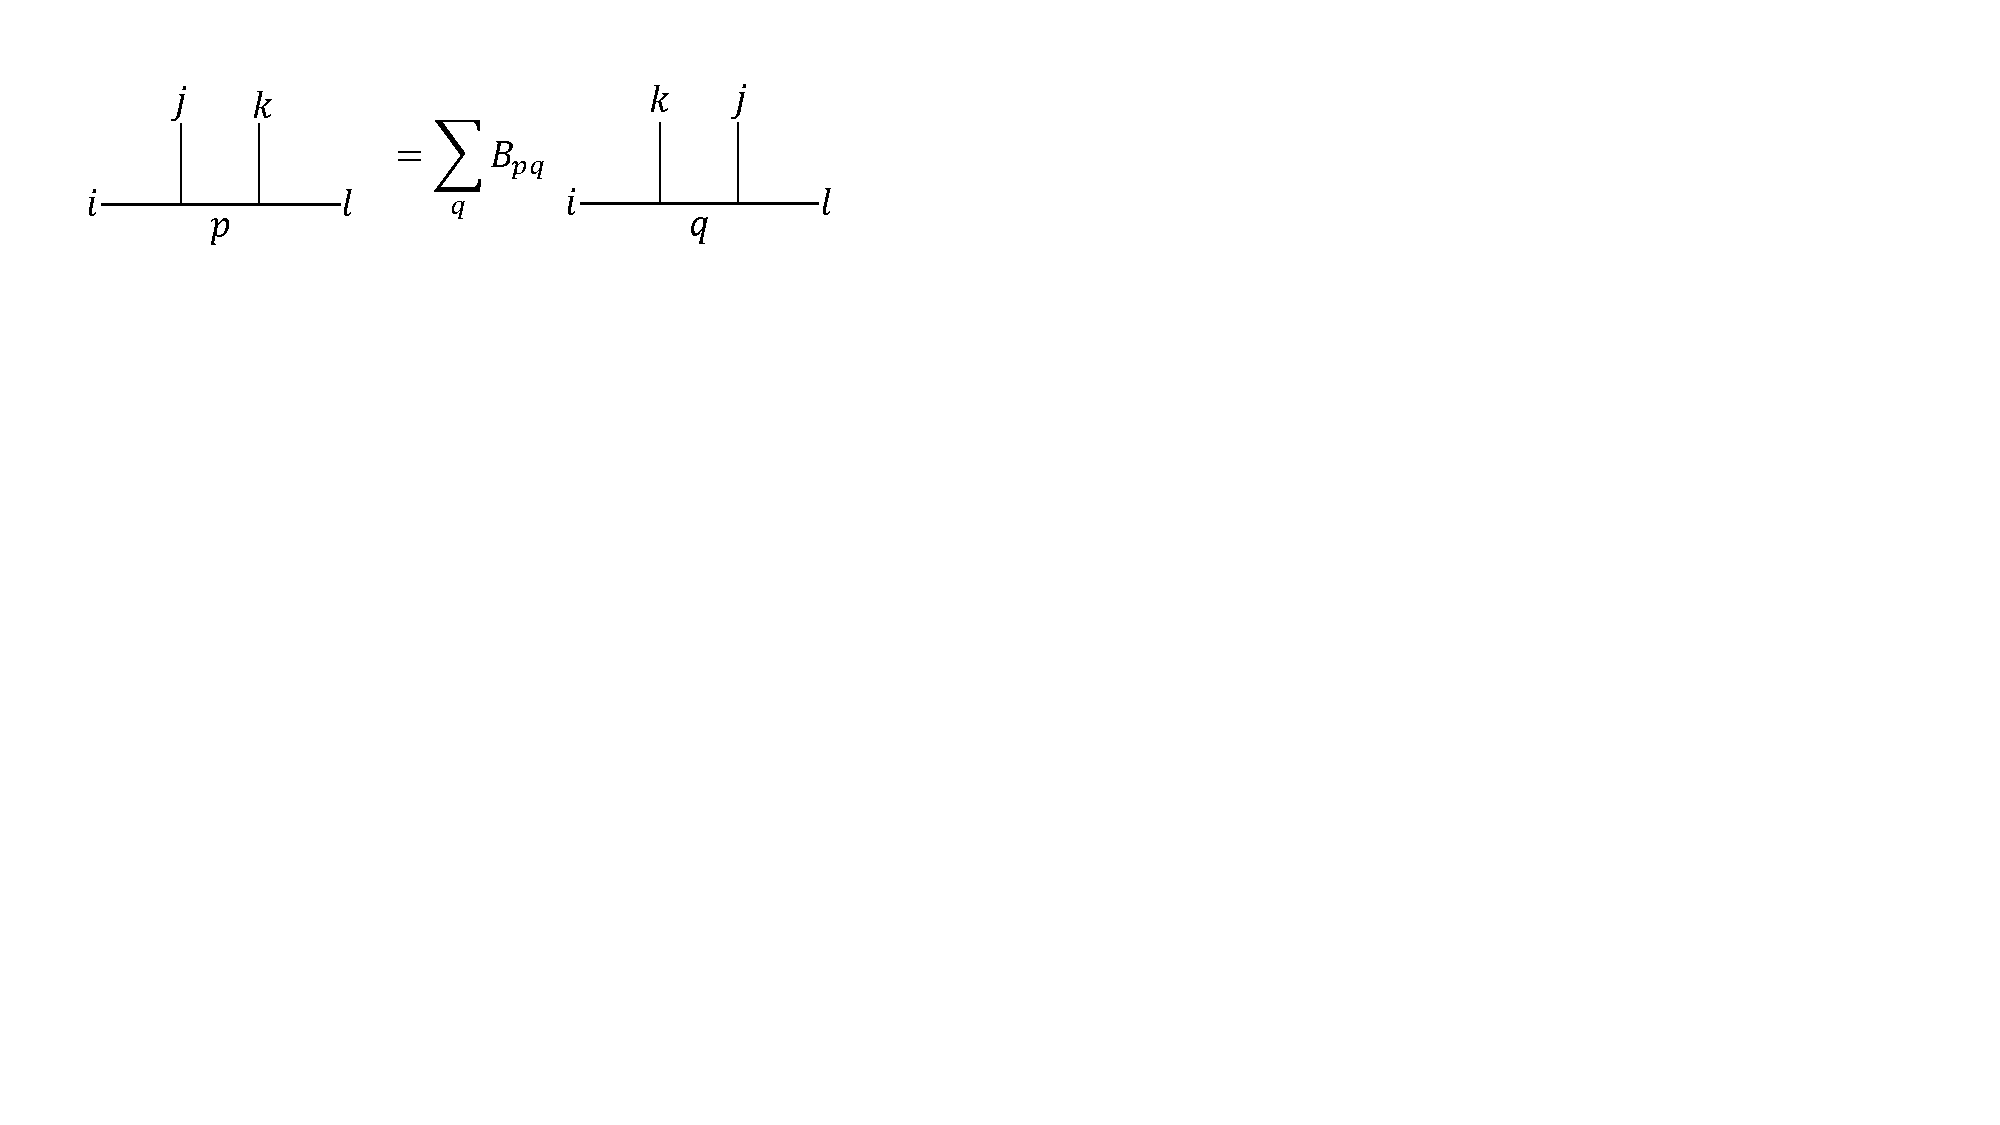
\includegraphics[width=0.8\linewidth]{figs/fig11.pdf}
\end{figure}
\begin{figure}[H]
	\centering
	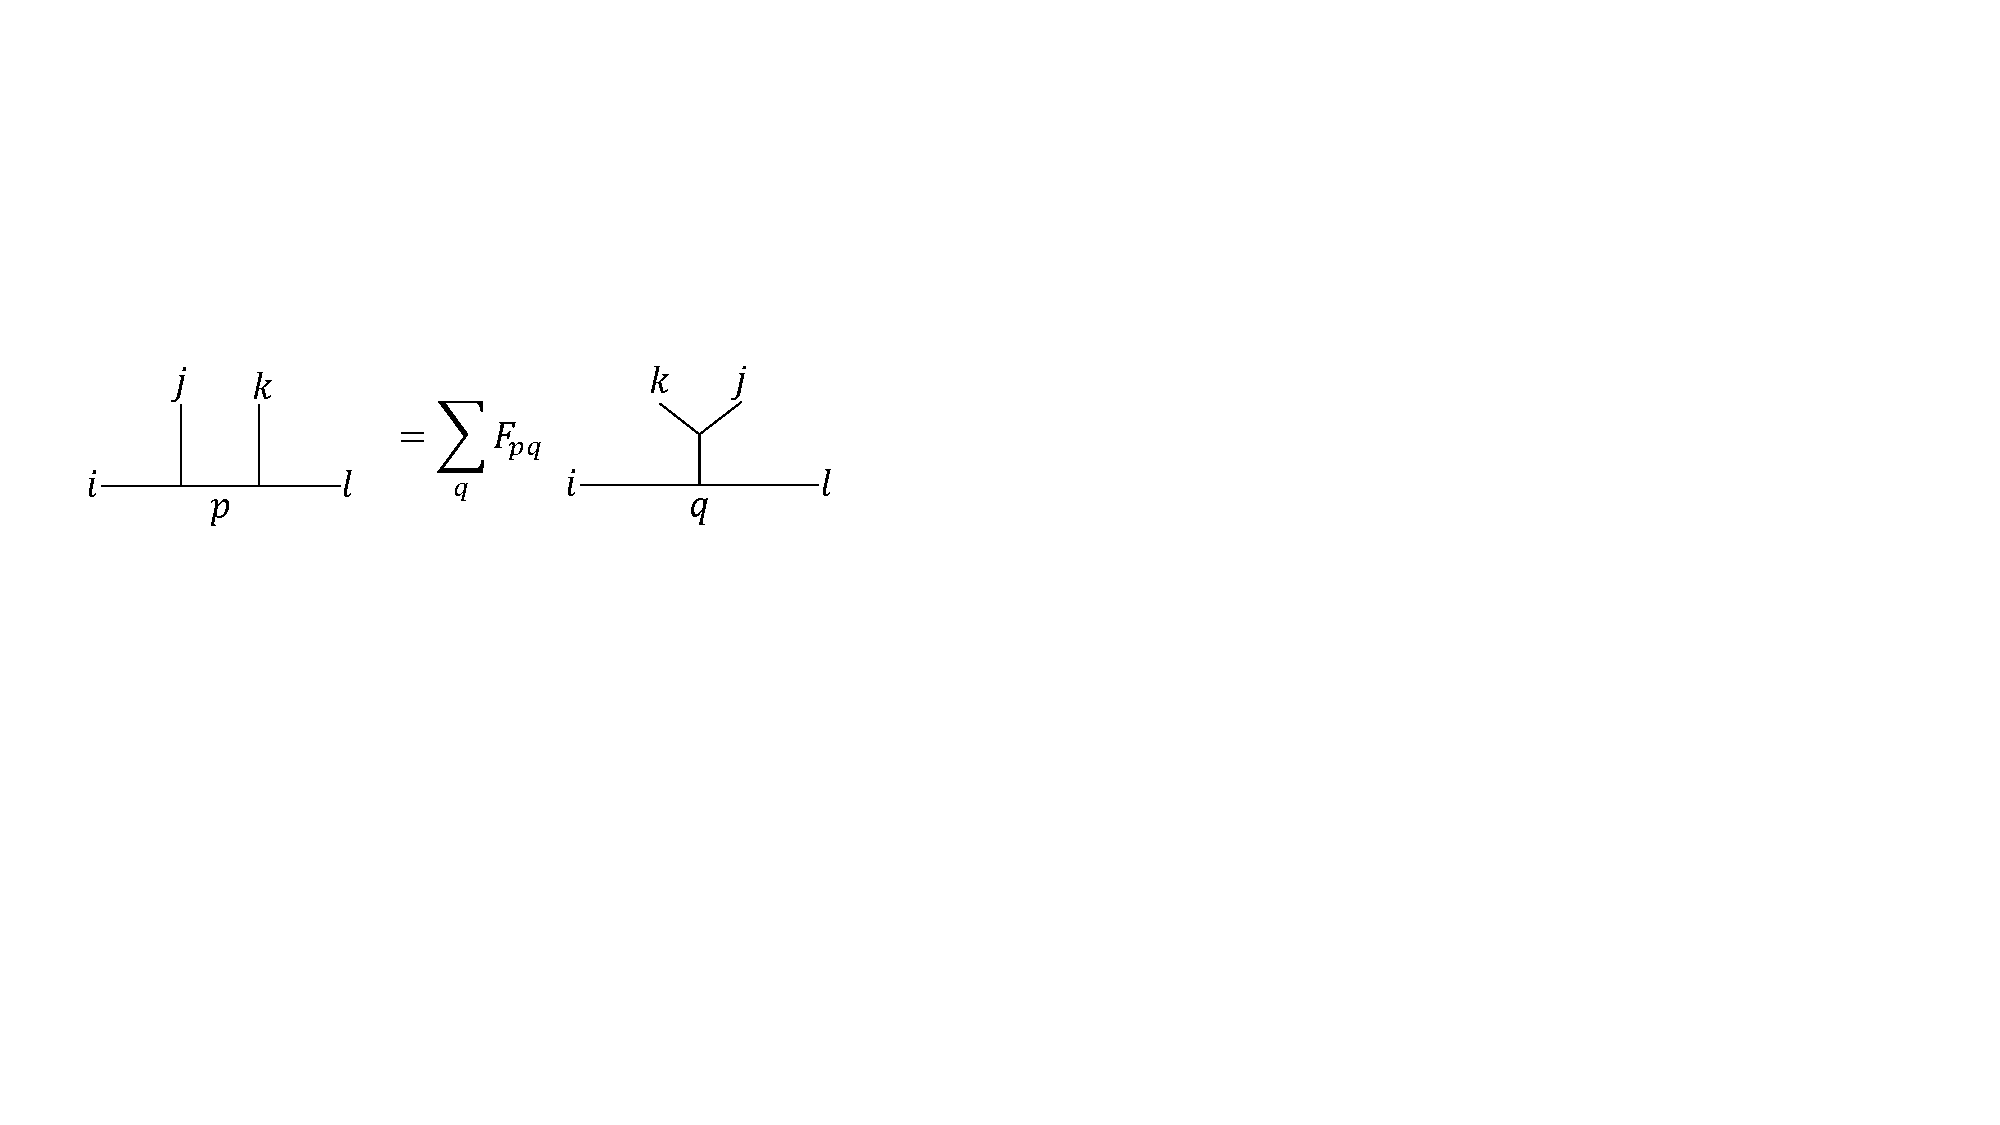
\includegraphics[width=0.8\linewidth]{figs/fig12.pdf}
\end{figure}
利用下面图表的交换性:
\begin{figure}[H]
	\centering
	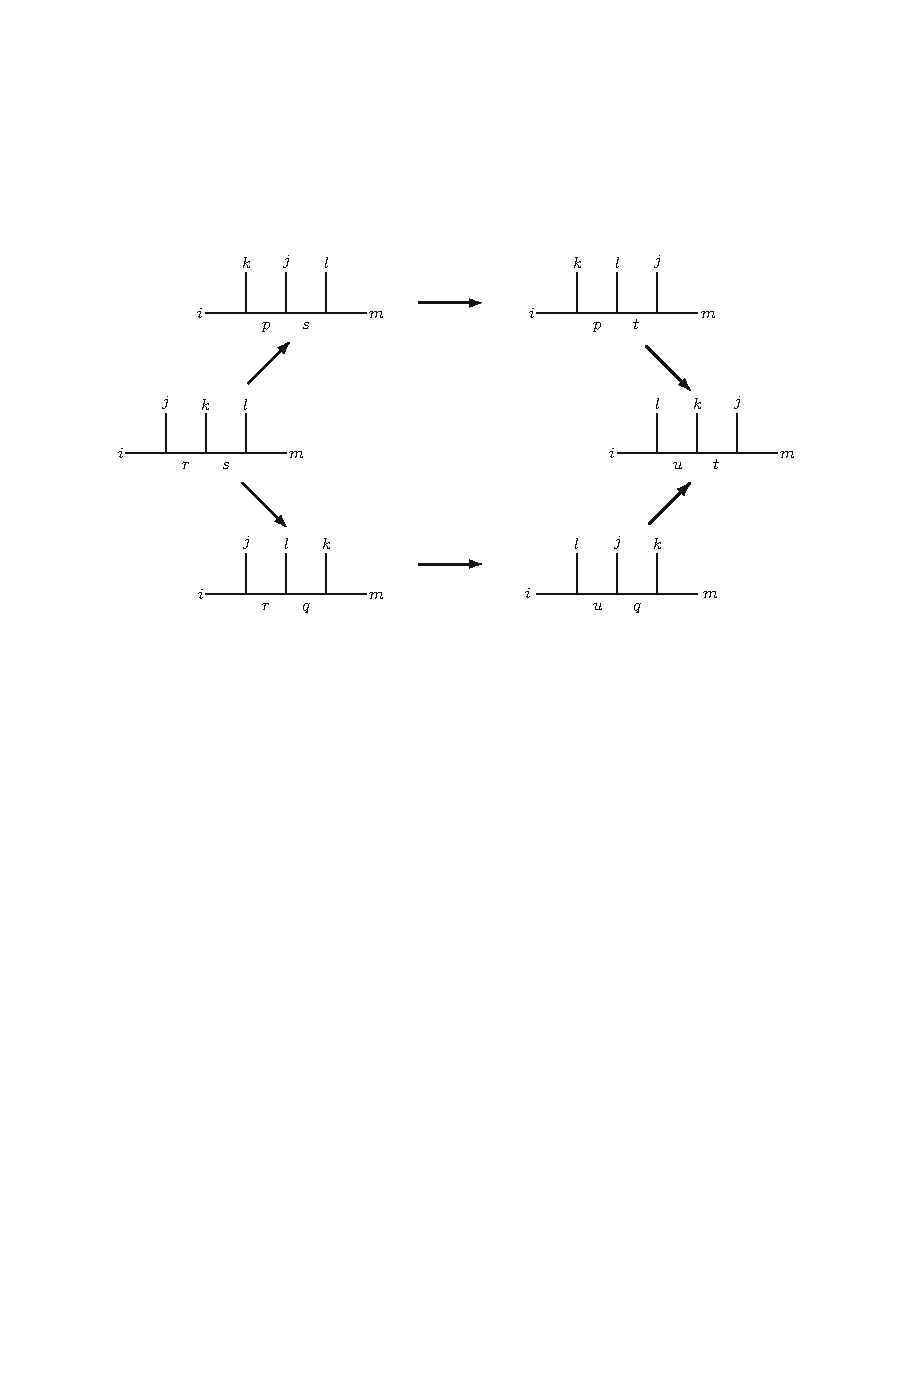
\includegraphics{figs/fig13.pdf}
\end{figure}
得到hexgon恒等式:
\begin{equation}
	\boxed{
		\sum_{p} B\left[\begin{array}{cc}
			j & k \\
			i & s
		\end{array}\right]_{r p} B\left[\begin{array}{cc}
			j & l \\
			p & m
		\end{array}\right]_{s t} B\left[\begin{array}{cc}
			k & l \\
			i & t
		\end{array}\right]_{p u}=\sum_{q} B\left[\begin{array}{cc}
			k & l \\
			r & m
		\end{array}\right]_{s q} B\left[\begin{array}{cc}
			j & l \\
			i & q
		\end{array}\right]_{r u} B\left[\begin{array}{cc}
			j & k \\
			u & m
		\end{array}\right]_{q t}
	}
\end{equation}
上面的方程非常像Yang-Baxter方程,所以CFT和可积性有很大的关联。但是注意上面这不是证明!就和YBE的图形化规则推导一样,只是便于计算和记忆。同样根据下面的图表交换:
\begin{figure}[H]
	\centering
	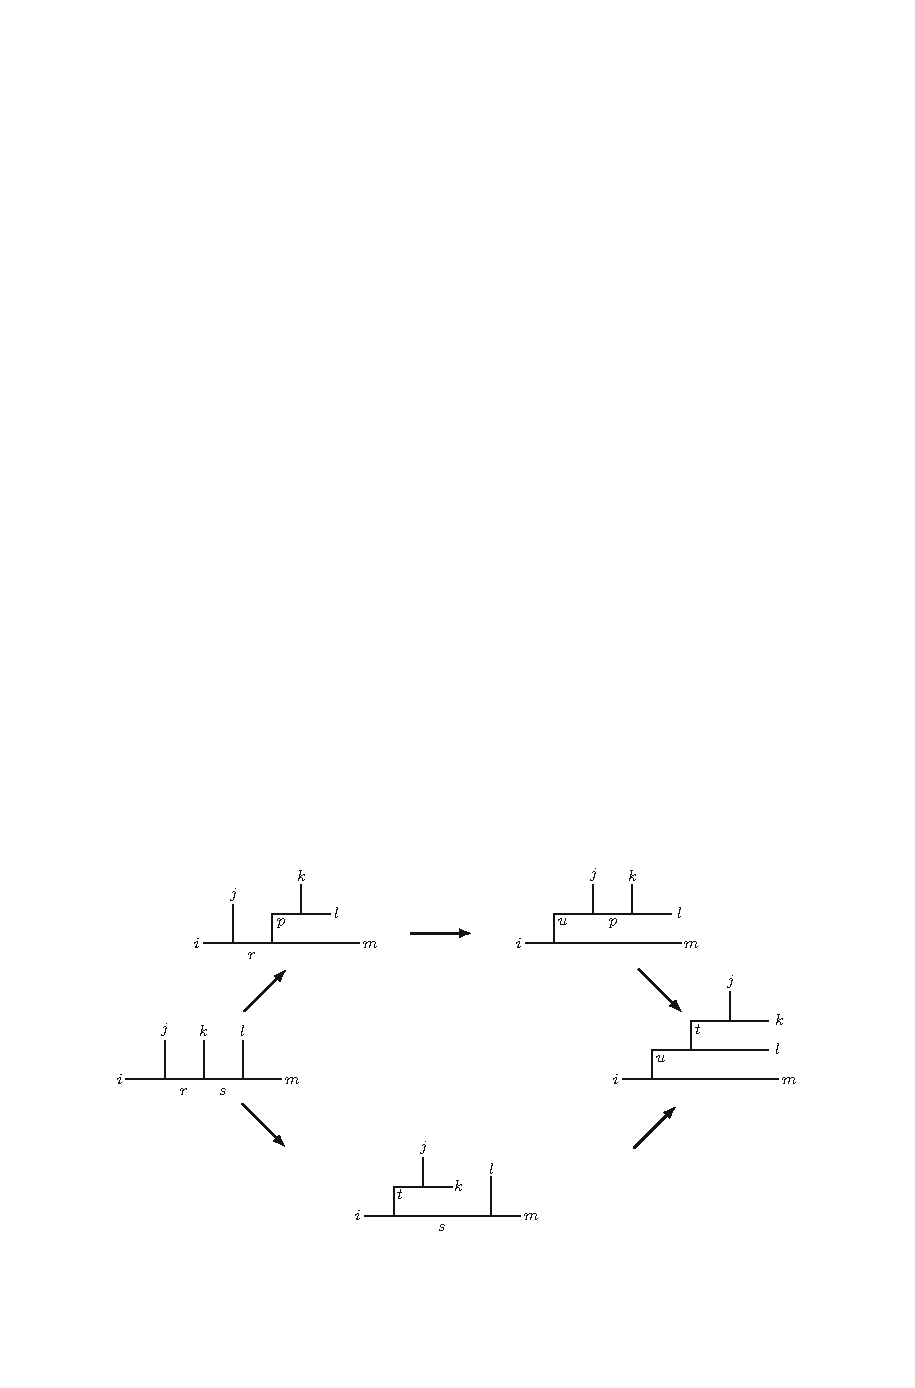
\includegraphics{figs/fig14.pdf}
\end{figure}
得到pentagon恒等式:
\begin{equation}
	\boxed{
		 F\left[\begin{array}{cc}
			j & k \\
			i & s
		\end{array}\right]_{r t} F\left[\begin{array}{cc}
			t & l \\
			i & m
		\end{array}\right]_{s u} =\sum_{p} F\left[\begin{array}{cc}
			k & l \\
			r & m
		\end{array}\right]_{s p} F\left[\begin{array}{cc}
			j & p \\
			i & m
		\end{array}\right]_{r u} F\left[\begin{array}{cc}
			j & k \\
			u & l
		\end{array}\right]_{p t}
	}
\end{equation}
\section{NOPs and Conformal family}
\subsection{Normal Ordered Products}
两个算符的OPE在两个算符的插入位置一样时会发散,这种发散就类似于一般QFT中的红外发散,因为空间无限大,所以真空零点能发撒,这种发散可以通过取算符的正规乘积(NOP)得到,共形场论也有这样的做法。我们先考虑\textbf{自由场},也就是$R(\phi\partial^n\phi)$最多只有一项是奇异的,\sn{对到QFT那边就是场的模式展开可以完全分离成产生算符和湮灭算符之和}那么我们直接减去真空期望值就去除了所有的发散项,所以NOP可以定义为:
\begin{definition}[NOPs]
	\begin{equation}
		:\phi_1(z)\phi_2(w):\equiv\left(\phi_1(z)\phi_2(w)-\left\langle{\phi_1(z)\phi_2(w)}\right\rangle\right):
	\end{equation}
	这里省略了所有的径向排序,记收缩:
	\begin{equation}
		\wick{\c \phi(z)\c \phi(w)}\equiv \left\langle{\phi_1(z)\phi_2(w)}\right\rangle
	\end{equation}
	缩并后是一个数,可以提出去。显然在$z\to w$后OPE的所有奇异性都被减除:
	\begin{equation}
		:\phi_1\phi_2:(w)\equiv\lim_{z\to w}\left(:\phi_1(z)\phi_2(w):\right)
	\end{equation}
\end{definition}
\begin{theorem}[Wick]
	\begin{equation}
		\boxed{
			\begin{aligned}
				\mathsf R[\Phi_{a_1}(x_1)\Phi_{a_2}(x_2)\cdots\Phi_{a_n}(x_n)]=\mathsf N\big[&\Phi_{a_1}(x_1)\Phi_{a_2}(x_2)\cdots\Phi_{a_n}(x_n)\\&+\left(\Phi_{a_1}\Phi_{a_2}\cdots\Phi_{a_n}\text{的所有可能缩并}\right)\big]
			\end{aligned}
		}
	\end{equation}
	由于正规序插入到真空态之间恒为0,所以任何没有完全缩并的项对真空期望值都没有贡献。
\end{theorem}
\begin{proof}
	关于Wick定理的证明可见任何一本正则量子化的QFT教材,比如余钊焕老师的讲义\footnote{\url{http://yzhxxzxy.github.io/cn/teaching.html}},这里只想强调定理本身依赖于前面对自由场的NOP定义。
\end{proof}
\begin{example}
	\begin{equation}
		\begin{aligned}\mathsf{R}(\Phi_a\Phi_b\Phi_c\Phi_d)&=\mathsf{N}\big(\Phi_a\Phi_b\Phi_c\Phi_d+\wick{\c \Phi_a\c\Phi_b\Phi_c\Phi_d}+\wick{\c\Phi_a\Phi_b\c\Phi_c\Phi_d}+\wick{\c\Phi_a\Phi_b\Phi_c\c\Phi_d}\\&\quad\quad+\wick{\Phi_a\c\Phi_b\c\Phi_c\Phi_d}+\wick{\Phi_a\c\Phi_b\Phi_c\c\Phi_d}+\wick{\Phi_a\Phi_b\c\Phi_c\c\Phi_d}\\&\quad\quad+\wick{\c\Phi_a\c\Phi_b}\wick{\c\Phi_c\c\Phi_d}+\wick{\c1\Phi_a\c2\Phi_b\c1\Phi_c\c2\Phi_d}+\wick{\c1\Phi_a\c2\Phi_b\c2\Phi_c\c1\Phi_d}\big)\end{aligned}
	\end{equation}
	计算的下一步是将所有收缩的项放在一起,未收缩的项放在一起,对于玻色场由于满足对易关系可以随便移动场的位置,这一步是trivial的,不过费米场因为满足反对易关系,所以交换两个场位置时会产生一个负号需要额外注意。
	
	左边减去右边,并取$x_a,x_b\to x$和$x_c,x_d\to y$的极限后得到两个NOP的时序积的Wick定理:
	\begin{equation}\label{33.6}
		\begin{aligned}
			\mathsf{R}\left[:\Phi_a\Phi_b:(x):\Phi_c\Phi_d:(y)\right]&=\mathsf{N}\big(\Phi_a\Phi_b\Phi_c\Phi_d+\wick{\c\Phi_a\Phi_b\c\Phi_c\Phi_d}+\wick{\c\Phi_a\Phi_b\Phi_c\c\Phi_d}\\&\quad\quad+\wick{\Phi_a\c\Phi_b\c\Phi_c\Phi_d}+\wick{\Phi_a\c\Phi_b\Phi_c\c\Phi_d}\\&\quad\quad+\wick{\c1\Phi_a\c2\Phi_b\c1\Phi_c\c2\Phi_d}+\wick{\c1\Phi_a\c2\Phi_b\c2\Phi_c\c1\Phi_d}\big)
		\end{aligned}
	\end{equation}
	这个计算实际上是非常一般的,他告诉我们计算NOP的时序积时跟没有NOP时一样计算,但是认为NOP内部的场之间的收缩为0。
\end{example}
\begin{remark}
	下面是一些比较有用的缩并等式:
	\begin{equation}
		\wick{\c A(z)\c{:B^{n}:}}(w)=n\wick{\c A(z)\c B(w)}:B^{n-1}(w):
	\end{equation}
	\begin{equation}
		\wick{\c A(z):\c {e}^{B(w)}:}=\wick{\c A(z)\c B(w)}:e^{B(w)}:
	\end{equation}
	\begin{equation}\label{33.9}
		\begin{aligned}
			\wick{:\c{e}^{A(z)}::\c{e}^{B(z)}:}&=\sum_{m,n,k}\frac{k!}{m!n!}\begin{pmatrix}m\\k\end{pmatrix}\begin{pmatrix}n\\k\end{pmatrix}[\wick {\c A(z)\c B(w)}]^k:A^{m-k}(w)B^{n-k}(w):\\&=\exp\left\{\wick{\c A(z)\c B(w)}\right\}:e^{A(w)}e^{B(w)}:\end{aligned}
	\end{equation}
\end{remark}
但是对于非自由场,NOP不能这么定义,比如$TT$的NOP照此定义,仍然发散,所以对于一般场的NOP应当定义成减去所有的奇异项。
\begin{definition}
	\begin{equation}
		\left(A(z)B(w)\right)\equiv A(z)B(w)-\wick{\c A(z)\c B(w)}
	\end{equation}
	这里$\wick{\c A(z)\c B(w)}$表示OPE的\textbf{所有}奇异部分。注意我们引入了文献中另外一种表示NOP的方式:$\left(\cdot\right)$。同样,定义:
	\begin{equation}
		\left(AB\right)(w)=\lim_{z\to w} \left(A(z)B(w)\right)
	\end{equation}
\end{definition}
将NOP其中一个场做洛朗展开,然后可以将OPE用NOP表达为:
\begin{theorem}[NOPs $\iff$ OPEs]
	\begin{equation}
		\phi(z)\chi(w)=\operatorname{sing.}+\sum_{n=0}^\infty\frac{(z-w)^n}{n!}N\big(\partial^n\phi\chi\big)(w)
	\end{equation}
	同样可以用OPE表达NOP:
	\begin{equation}
		N\left(\phi\chi\right)(w)=\oint_{\mathcal{C}(w)}\frac{dz}{2\pi i}\frac{\phi(z)\chi(w)}{z-w}
	\end{equation}
\end{theorem}
考虑NOP的Laurent模:
\begin{equation}
	\begin{aligned}N\left(\phi\chi\right)&(w)=\sum_{n\in\mathbb{Z}}w^{-n-h^\phi-h^\chi}N\left(\phi\chi\right)_n,\\N\left(\phi\chi\right)_n&=\oint_{\mathcal{C}(0)}\frac{dw}{2\pi i}w^{n+h^\phi+h^\chi-1}N\left(\phi\chi\right)(w)\end{aligned}
\end{equation}
\begin{theorem}
	\begin{equation}
		\boxed{
		N\left(\phi\chi\right)_{n}=\sum_{k>-h^{\phi}}\chi_{n-k}\phi_{k}+\sum_{k\leq-h^{\phi}}\phi_{k}\chi_{n-k}
		}
	\end{equation}
\end{theorem}
\begin{proof}
	\begin{equation}
		\begin{aligned}N\left(\phi\chi\right)_n&=\oint_{C(0)}\frac{dw}{2\pi i}w^{n+h^\phi+h^{\lambda}-1}\oint_{C(w)}\frac{dz}{2\pi i}\frac{\phi(z)\chi(w)}{z-w}\\&=\underbrace{\oint\frac{dw}{2\pi i}w^{n+h^\phi+h^{\lambda}-1}\Big(\underbrace{\oint_{|z|>|w|}\frac{dz}{2\pi i}\frac{\phi(z)\chi(w)}{z-w}}_{\mathcal{I}_1}}_{\mathcal{I}_2}-\oint_{|z|<|w|}\frac{dz}{2\pi i}\frac{\chi(w)\phi(z)}{z-w}\Big)\end{aligned}
	\end{equation}
	计算$\mathcal{I}_1$得到:
	\begin{equation}
		\begin{aligned}
			\mathcal{I}_{1}& =\oint_{|z|>|w|}\frac{dz}{2\pi i}\frac{1}{z-w}\sum_{r,s}z^{-r-h^{\phi}}w^{-s-h^{\chi}}\phi_{r}\chi_{s}  \\
			&=\oint_{|z|>|w|}\frac{dz}{2\pi i}\left.\frac1z\sum_{p\geq0}\left(\frac wz\right)^p\sum_{r,s}z^{-r-h^\phi}w^{-s-h^\chi}\phi_r\chi_s\right.  \\
			&=\oint_{|z|>|w|}\frac{dz}{2\pi i}\sum_{p\geq0}\sum_{r,s}z^{-r-h^\phi-p-1}w^{-s-h^\chi+p}\phi_r\chi_s.
		\end{aligned}
	\end{equation}
	频繁利用Cauchy积分公式得到:
	\begin{equation}
		\begin{aligned}
			\mathcal{I}_2&=\oint\frac{dw}{2\pi i}\sum_{p\geq0}\sum_sw^{-s-h^x+p+n+h^\phi+h^x-1}\phi_{-h^\phi-p}\chi_s\\
			&=\sum_{p\geq0}\phi_{-h^\phi-p}\chi_{h^\phi+n+p}=\sum_{k\leq-h^\phi}\phi_k\chi_{n-k}
		\end{aligned}
	\end{equation}
	对另外一项也同样计算就可以证明这个及其重要的等式了。
\end{proof}
这个等式其实非常好理解,从前面对CFT的希尔伯特空间构造可以看到,一个场的Laurent模当$n>-h$时是湮灭算符,$n\leq-h$时是产生算符,所以这个等式的含义就是相对$\phi$而言将所有的产生算符排在前面,湮灭算符放在后面,这正是在QFT中对NOP最naive的定义!

另外,NOP与OPE最大的不同是他并不满足交换律和结合律,这也意味着对多个算符的NOP定义有歧义\sn{对于自由场,前面的定义还是well-define的},往往选取的是下面的嵌套定义:
\begin{equation}
	(ABC\cdots DE)\equiv(A(B(C(\cdots(DE))))))
\end{equation}
另外,Wick定理也失效了,不过我们有下面的等式:
\begin{theorem}[Generalized Wick]
	\begin{equation}\label{wick}
		\boxed{
			{A(z)(BC)}(w)=\frac1{2\pi i}\oint_{\mathcal{C}(w)}\frac{dx}{x-w}\left\{\wick{\c A(z)\c B}(x)C(w)+B(x)\wick{\c A(z)\c C}(w)\right\}+\text{regular}
		}
	\end{equation}
\end{theorem}
上式是对自由场的下面特殊的Wick定理的相互作用推广:
\begin{equation}
	\phi_1(x):\phi_2\phi_3:(y)=\wick{\c\phi_1(x)\c\phi_2(y)}:\phi_3(y):+\wick{\c\phi_1(x)\c\phi_3(y)}:\phi_2(y):+\underbrace{:\phi_1(x)\phi_2(y)\phi_3(y):}_{\text{regular}}
\end{equation}
还可以证明,虽然结合律失效了,但是有下面等式:
\begin{theorem}[Rearrangement Lemma]
	\begin{equation}
		((AB)E)-(A(BE))=(A([E,B]))+(([E,A])B)+([(AB),E])
	\end{equation}
	$E$一般取为$(CD)$。
\end{theorem}
$T$不是初级场,$N(TT)$也不是初级场,但是下面定义的$\mathcal{N}(TT)$是共形权为$(4,0)$的初级场:
\begin{equation}
	\boxed{
		\mathcal{N}(TT)=N\left(TT\right)-\frac3{10}\partial^2T
	}
\end{equation}
后面会用到这个式子。
\subsection{Verma module}
从真空态出发,将$L_n$作为产生算符作用上去,得到的一系列态成为Verma模:
\begin{definition}[Verma Module]
	\begin{equation}
		\boxed{
			\left\{L_{k_1}\ldots L_{k_n}|0\rangle|k_i\leq-2\right\}
		}
	\end{equation}
	中的元素称为Verma Module。
\end{definition}
根据态算符对应,每一个Verma Module都会对应一个场(不一定是初级场),可以证明这些场一定是能动张量或者其偏导或者它们的NOP:
\begin{equation}
	\boxed{
		F\in\left\{T,\partial T,\ldots,N(\ldots)\right\}
	}
\end{equation}
\subsection{Descendant states}
前面是考虑一个真空态开始往上构造其它态,由于:
\begin{equation}
	L_n\left|\phi\right\rangle=\left[L_n,\phi_{-h}\right]\left|0\right\rangle=\left(h\left(n+1\right)-n\right)\phi_{-h+n}\left|0\right\rangle=0,\quad n>0
\end{equation}
所以初级场作用在真空态上构造的$\ket{\phi}$也比较特殊,和真空态一样被所有的$L_n$湮灭算符湮灭,所以也可以考虑从$\ket{\phi}$开始构造其它态:
\begin{definition}[Descendant States]
	\begin{equation}
		\boxed{
			\left\{L_{k_1}\ldots L_{k_n}|\phi\rangle:\mathrm{~}k_i\leq-1\right\}
		}
	\end{equation}
	其中$\phi$是任意一个初级场。这些态称为初级场的次级态(descendant states)。
\end{definition}
\begin{table}[H]
\centering
\begin{tabular}{lrc}
	\text { Field } & \text { State } & \text { Level } \\
	\hline \hline$ \phi(z)$& $\phi_{-h}|0\rangle=|h\rangle$ & $0 $\\
	\hline $\partial \phi $& $L_{-1} \phi_{-h}|0\rangle $& $1$ \\
	\hline$ \partial^{2} \phi $& $L_{-1} L_{-1} \phi_{-h}|0\rangle $& $2 $\\
	$N(T \phi)$ &$ L_{-2} \phi_{-h}|0\rangle$ & 2 \\
	\hline $\partial^{3} \phi$ & $L_{-1} L_{-1} L_{-1} \phi_{-h}|0\rangle$ & $3$ \\
	$N(T \partial \phi)$ &$ L_{-2} L_{-1} \phi_{-h}|0\rangle $&$ 3$ \\
	$N(\partial T \phi) $& $L_{-3} \phi_{-h}|0\rangle $& $3$ \\
	\hline \ldots & \ldots & \ldots
\end{tabular}
\caption{次级态和次级场之间的对应}
\label{descendant}
\end{table}
同样根据态算符对应,这些态也会对应到一些场,根据上面的表就可以猜到是:
\begin{equation}
	\boxed{
		\left[\phi(z)\right]:=\left\{\phi,\partial\phi,\partial^2\phi,\ldots,N(T\phi),\ldots\right\}
	}
\end{equation}
我们成为$\phi$的Conformal Family。Verma Module是直接真空态生成来的,真空态对应$h=0$,可以用$[1]$来标记这个特殊的Conformal Family。

注意到在上面的表中我们写下来对应的Level,注意到$L_0$可看作体系的哈密顿量,真空态对应能量0,初级场$\ket{h}$对应能量$h$,而作用$L_{-k}$上去会把能量加$k$,所以这就跟量子力学中谐振子问题作用产生算符得到更高能级的态一样。只不过这里能级都是简并的,而简并态数目的计数在后面的环面CFT配分函数构造上有很大的作用,对于Verma module(真空态毕竟唯一),或者$\ket{h}$本身不简并的Conformal Family来说,设$P(N)$是第$N$个Level简并度,则其有下面的生成函数:
\begin{equation}
	\boxed{
		\prod_{n=1}^\infty\frac1{1-q^n}=\sum_{N=0}^\infty P(N)q^N
	}
\end{equation}

次级态和次级场之间用NOP对应,而NOP天然的和OPE有对应,所以实际上我们可以用OPE的围道积分来表示:
\begin{theorem}
	用$\widehat{L}_{-n}\phi(w)$表示$L_{-n}\ket\phi$对应的次级场,那么:
	\begin{equation}\label{eq:33.30}]
		\boxed{
			\widehat{L}_{-n}\phi(w)=\oint_{\mathcal{C}(w)}\frac{dz}{2\pi i}\frac1{(z-w)^{n-1}}T(z)\phi(w)
		}
	\end{equation}
\end{theorem}
\begin{proof}
	利用态算符对应,取$w\to 0$的极限就能看出正确性了。代入OPE实际计算几个例子也能得到表\ref{descendant}的结果。
\end{proof}
现在我们来证明CFT自举里面非常重要的一个微分方程,核心目的是将次级态和其他初级场的关联函数用其他初级场的关联函数来表示。
\begin{theorem}
	$\phi,\phi_1,\ldots,\phi_N$是初级场,则:
	\begin{equation}\label{33.31}
		\boxed{
			\begin{gathered}
				\left\langle\widehat{L}_{-n}\phi(w)\phi_{1}(w_{1})\ldots\phi_{N}(w_{N})\right\rangle=\mathcal{L}_{-n}\langle\phi(w)\phi_{1}(w_{1})\ldots\phi_{N}(w_{N})\rangle  \\
				\text{Where,}\qquad\mathcal{L}_{-n}=\sum_{i=1}^N\left(\frac{(n-1)h_i}{(w_i-w)^n}-\frac1{(w_i-w)^{n-1}}\partial_{w_i}\right)
			\end{gathered}
		}
	\end{equation}
\end{theorem}
\begin{proof}
	\begin{equation}
		\begin{aligned}
			&\left\langle\widehat{L}_{-n}\phi(w)\phi_1(w_1)\ldots\phi_N(w_N)\right\rangle  \\
			=&\oint_{\mathcal{C}(w)}\frac{dz}{2\pi i}\left.(z-w)^{1-n}\left\langle\left(T(z)\phi(w)\right)\phi_1(w_1)\ldots\phi_N(w_N)\right\rangle\right.  \\
			=&-\sum_{i=1}^N\oint_{\mathcal{C}(w_i)}\frac{dz}{2\pi i}\left.(z-w)^{1-n}\left\langle\phi(w)\phi_1(w_1)\ldots\left(T(z)\phi_i(w_i)\right)\ldots\phi_N(w_N)\right\rangle\right.  \\
			=&-\sum_{i=1}^N\oint_{\mathcal{C}(w_i)}\frac{dz}{2\pi i}\left(z-w\right)^{1-n}\times  \\
			&\times\left(\frac{h_i}{(z-w_i)^2}+\frac1{z-w_i}\partial_{w_i}\right)\left\langle\phi(w)\phi_1(w_1)\ldots\phi_N(w_N)\right\rangle  \\
			=&-\sum_{i=1}^N\left((1-n)\left(w_i-w\right)^{-n}h_i+\left(w_i-w\right)^{1-n}\partial_{w_i}\right)\left<\phi(w)\phi_1(w_1)\ldots\phi_N(w_N)\right>
		\end{aligned}
	\end{equation}
	上面证明中第二个等号利用了全平面内极点留数只和为0,第三个等号利用了初级场OPE。
\end{proof}
\section{Representations of the Virasoro Algebra}
现在来从群表示的观点看下我们前面的Verma Module和Conformal Family实在做什么。前面反复强调如果我们有了一个理论的对称代数,那么确定其希尔伯特空间就是在找群表示。最简单的CFT就是只有Virasoro代数作为其对称代数,由于这时左右模完全分离,所以我们可以先分开讨论,然后$\bigoplus_{\{h,\bar h\}} V_{c,h}\otimes V_{c,\bar h}$就构成了整个表示空间\sn{也正因为完全分离,这里$h,\bar h$直积时无特殊要求,后面玻色子我们会看到一个有要求的最简单的例子。}。

我们要找的表示是所谓最高权表示,从量子力学的角度去想,构造谱的第一步是去找CSCO,由于理论没有其他对称性,也就是说没有其他力学量和$L_0$对易,所以我们期望构造的谱是$L_0$的本征值。进一步,由于$\{L_n,n\geq0\}$构成了理论的湮灭算符,所以我们先找到被所有湮灭算符湮灭的那些态:
\begin{equation}
	\begin{aligned}L_n\left|h\right\rangle&=0\quad\text{for}\quad n>0,\\L_0\left|h\right\rangle&=h\left|h\right\rangle\end{aligned}
\end{equation}
找到了所有的最高权之后,下一步就是将产生算符$\{L_{n},n<0\}$作用到上面构造能量更高的态:\sn{这些态都是$L_0$的本征态,但是我们并不用$\ket{h+k}$这样的记号标记他们,因为要和最高权区分。}
\begin{equation}
	L_{-1}\ket{h},\quad L_{-2}\ket{h},\quad L_{-1}L_{-1}\ket{h},\quad L_{-3}\ket{h},\quad\ldots
\end{equation}
不难发现,最高权就是真空态和理论中的初级态,而其他用产生算符构造的态就是Verma module和descendant states。

但是这只是从数学上构造出了这些态,真正物理的态最大的特点就是可归一化,所以那些模方为0的态要被剔除出去,比如说前面在构造Verma Module时,就没有把$L_{-1}\ket{0}$算进去,后面我们会进一步阐明如何找到其它的模方为0的态。进一步如果要求理论是幺正的,那些模方为负数的表示还要整个剔除掉。\sn{注意,幺正性要求那些有模方为负数的次级态的表示是被禁闭的,而不是像模方为0的态稍微剔除一下就好。}

如果理论还存在更大的对称性,这个时候CSCO就会加入其他的和${L_0}$对易的算符,谱将会同时对角化CSCO中的算符,即最高权现在由更多量子数标记$\ket{h,q}$。而且产生湮灭算符也不只有$\{L_{n},n<0\}$了,构造次级态还需要用理论中其他的产生湮灭算符去作用。这在数学上本身就是个非常麻烦的事情,后面我们并不追求数学上的一般性和严谨性,只是给些例子。

\section{Free CFT}
学习CFT最好的方式是给出一些具体的例子,首先我们考虑最简单的自由CFT。
\subsection{Free Bosons}
自由玻色场可以从圆柱上定义的标量场量子化后得来,这里直接给出二维CFT的版本\sn{已经做了Wick转动,$\kappa$是弦论来的耦合常数}:
\begin{equation}
	\begin{aligned}
		\text{S}& =\frac1{4\pi\kappa}\int dzd\overline{z}\sqrt{|g|}g^{ab}\partial_aX\partial_bX  \\
		&\xleftarrow{\kappa=1}\frac1{4\pi}\int dzd\overline{z}\partial X\cdot\overline{\partial}X
	\end{aligned}
\end{equation}
其中度规是从圆柱上的平直度规转到复平面上的度规:
\begin{equation}
	\left.g_{ab}=\left[\begin{array}{cc}0&\frac{1}{2z\overline{z}}\\\frac{1}{2z\overline{z}}&0\end{array}\right.\right],\quad g^{ab}=\left[\begin{array}{cc}0&2z\overline{z}\\2z\overline{z}&0\end{array}\right]
\end{equation}
再次强调CFT的定义根本不需要拉氏量,这里只是更场论一点的出发方式。直接读出运动方程:\sn{这也说明$X(z,\bar z)$总是可以写成全纯和反全纯部分之和}
\begin{equation}
	\partial\overline{\partial}X(z,\overline{z})=0
\end{equation}
可以定义下面两个手征场:
\begin{equation}\label{35.4}
	j(z)=i\partial X(z,\overline z),\quad\bar j(\overline z)=i\overline\partial X(z,\overline z)
\end{equation}
还可以读出传播子$K\equiv\left\langle{X(z,\bar z)X(w,\bar w)}\right\rangle$:
\begin{equation}
	\partial_z\partial_{\overline{z}}K(z,\overline{z},w,\overline{w})=-2\pi\delta^{(2)}(z,-w)\Rightarrow K=-\log\left|z-w\right|^2
\end{equation}
这直接说明了$X$不是初级场,但是:
\begin{equation}
	\left\langle j(z)j(w)\right\rangle=\frac{1}{(z-w)^2}
\end{equation}
说明了$j(z)$是$h=1$的初级场,也得到了OPE:\sn{由于OPE的最奇异项只能是二次的,而一次的又破坏了$z\leftrightarrow w$的对称性。}
\begin{equation}\label{35.7}
	\boxed{
		j(z)j(w)=\partial_z X(z)\partial_w X(w)=\frac{1}{(z-w)^2}+\ldots
	}
\end{equation}
根据OPE很容易算出对易关系:
\begin{equation}
	\boxed{
		\begin{bmatrix}j_m,j_n\end{bmatrix}= m\delta_{m+n,0}
	}
\end{equation}
根据$j$是共形权为1的初级场很容易证明作用量的确是共形不变的\sn{不少文献数量纲之后根据尺度不变性直接说明共形不变,绝大多数情况下这没问题,甚至一度让人们觉得尺度不变蕴含共形不变。但是上世纪八十年代Polchinski就研究了反例\cite{Polchinski:1987dy}}。下面演示如何通过作用量确定CFT中最关键的能动张量:
\begin{equation}
	T_{ab}=-4\pi~\gamma\frac1{\sqrt{|g|}}\frac{\delta\mathcal{S}}{\delta g^{ab}}
\end{equation}
这里$\gamma$是待定的归一化系数,利用上式计算得到:\sn{$\delta\sqrt{|g|}=-\frac12\sqrt{|g|}g_{ab}\delta g^{ab}$}
\begin{equation}
	T_{zz}=-\gamma\partial X\partial X,\quad\quad T_{z\overline{z}}=T_{\overline{z}z}=0
\end{equation}
下面最重要的一步就是取正规乘积,这相当于把理论的零点能shift掉:
\begin{equation}
	T(z)=-\gamma N(\partial X\partial X)(z)=\gamma N(jj)(z)
\end{equation}
定$\gamma$的方式有很多,重点就是其洛朗模$L_n$要满足Virasoro代数,$L_n$和初级场的洛朗模之间对易关系要有正确的形式\ref{31.27},或者是能动张量和初级场的OPE有\ref{31.14}的形式,我们主要来看这种方法:\sn{\ref{35.7}得知$\wick{\c j(z)\c j(w)}=\frac{1}{(z-w)^2}$}
\begin{equation}
	\begin{aligned}
		\wick{\c T(z)\c j(w)}&=\gamma \wick{\c N(jj)(z)\c j(w)}=\gamma \wick{\c j(w)\c N(jj)(z)}\\
		&=\frac{\gamma}{2\pi i}\oint_{\mathcal{C}(z)}\frac{dx}{x-z}\left\{\wick{\c j(w)\c j(x)}j(z)+j(x)\wick{\c j(w)\c j(z)}\right\}\\
		&=\frac{2\gamma}{(z-w)^2}j(z)\\
		&=\frac{2\gamma}{(z-w)^2}j(w)+\frac{2\gamma}{z-w}\partial j(w)
	\end{aligned}
\end{equation}
最后一步使用泰勒展开并丢掉Regular部分。和\ref{31.14}对比便知道$\gamma=\frac{1}{2}$:
\begin{equation}
	\boxed{
		T(z)=\frac{1}{2}N(jj)(z)
	}
\end{equation}
\begin{equation}\label{35.14}
	L_n=\frac{1}{2}\left.N(jj)_n=\frac{1}{2}\sum_{k>-1}j_{n-k}\left.j_k+\frac{1}{2}\right.\sum_{k\leq-1}j_k\left.j_{n-k}\right.\right. 
\end{equation}
下面再来阐明如何计算中心荷,比较简单的方式是利用$\langle0|L_{+2}L_{-2}|0\rangle=\langle0|[L_2,L_{-2}]|0\rangle=\frac c2$,为了继续熟悉Wick定理,我们根据$TT$ OPE来计算:
\begin{equation}
	\begin{aligned}
		T(z)T(w)&=\frac{1}{4}R\left[:jj:(z):jj:(w)\right]+\cdots\\
		&=\frac{1}{4}\wick{\c j(z)\c j(w)}:j(z)j(w):\times 2+\frac{1}{4}\wick{\c j(z)\c j(w)}\cdot\wick{\c j(z)\c j(w)}\times 2+\cdots\\
		&=\frac{1}{(z-w)^2}:j(z)j(w):+\frac{\frac{1}{2}}{(z-w)^4}+\cdots\\
		&=\frac{1}{(z-w)^2}:jj:(w)+\frac{1}{z-w}\partial_w :jj:(w)\times\frac{1}{2}+\frac{\frac{1}{2}}{(z-w)^4}+\cdots\\
		&=\frac{\frac{1}{2}}{(z-w)^4}+\frac{2T(w)}{(z-w)^2}+\frac{\partial_w T(w)}{z-w}+\cdots
	\end{aligned}
\end{equation}
这里利用了自由场的Wick定理\ref{33.6}进行计算,倒数第二个等号利用了$j(z)$泰勒展开。与\ref{TT}对比得到:
\begin{theorem}
	自由玻色场CFT的中心荷$\boxed{c=1}$
\end{theorem}
如果理论是$N$个无相互作用的Boson场,那么中心荷是$c=N$。所以中心荷某种程度上可以理解为理论的自由度个数。
\subsubsection{Vertex Operator}
虽然从CFT的角度来看我们更关心$j$,但是从弦的角度来看$X$是更基本的,利用\ref{35.7}洛朗展开后积分得到:
\begin{equation}\label{35.16}
	\left.X(z,\overline{z})=x_0-i\left(\begin{array}{c}j_0\ln z+\overline{j}_0\ln\overline{z}\\\end{array}\right.\right)+i\sum_{n\neq0}\frac1n\left(\begin{array}{c}j_nz^{-n}+\overline{j}_n\overline{z}^{-n}\\\end{array}\right)
\end{equation}
根据$X(e^{2\pi i}z,e^{-2\pi i}\bar z)=X(z,\bar z)$有:
\begin{equation}\label{35.17}
	\boxed{
		j_0=\bar j_0
	}
\end{equation}
这个等式是后面构造正确的希尔伯特空间的关键。从自由场模式展开的观点来看,这些$z^n$模对到圆柱那边就是傅里叶展开,所以$j_n$就是理论的产生湮灭算符。而$j_0$实际上对应质心的正则动量$\pi_0$:
\begin{equation}
	\pi_0=\frac1{4\pi}\int_0^{2\pi}dx^1\frac{\partial X{\left(x^0,x^1\right)}}{\partial{\left(-ix^0\right)}}=\frac{j_0+\overline{j}_0}2=j_0
\end{equation}
$x_0$对应弦的质心。按照正则量子化应当有$[x_0,\pi_0]=i$。这样来看\ref{35.14}就分成了质心的动能和弦上激发能,相对质心能量两部分。
\begin{equation}
	L_0=\frac12~j_0~j_0+\frac12~\sum_{k\geq1}j_{-k}~j_k+\frac12~\sum_{k\leq-1}j_k~j_{-k}
\end{equation}
\begin{definition}[Vertex Operator]
	虽然$X$本身不是初级场,但是总可以定义下面的顶点算符:
	\begin{equation}
		\boxed{
			V(z)=:e^{i\alpha X(z)}:
		}
	\end{equation}
	他是共形权为$\left(\frac{\alpha^2}{2},0\right)$的初级场,反全纯部分也可以类似定义。
\end{definition}
\begin{proof}
	利用Wick定理得到下面的OPE:
	\begin{equation}
		\partial\varphi(z):\varphi^n:(w)=\frac{-n}{z-w}:\varphi^{n-1}:(w)
	\end{equation}
	将顶点算符泰勒展开得到:
	\begin{equation}\label{35.21}
		\begin{aligned}
			\wick{\c j(z)\c V_{\alpha}(w)}& \begin{aligned}=\sum_{n=0}^\infty\frac{-in}{z-w}\frac{(i\alpha)^n}{n!}:\varphi^{n-1}:(w)\end{aligned}  \\
			&=\frac{\alpha}{z-w} V_\alpha(w)
		\end{aligned}
	\end{equation}
	再计算与$T$的OPE:\footnote{计算中并没有直接去用\ref{35.21},想想这是为什么?可以参考\url{https://physics.stackexchange.com/questions/398365/ope-double-contractions-between-t-and-eikx}}
	\begin{equation}
		\begin{aligned}
			\wick{\c T(z)\c V_{\alpha}(w)}
			=&\frac{1}{2}\sum_{n=0}^\infty\frac{(i\alpha)^n}{n!}:\partial\varphi(z)\partial\varphi(z)::\varphi(w,\bar{w})^n: \\
			=&\frac1{2}\frac1{(z-w)^2}\sum_{n=2}^\infty\frac{(i\alpha)^n}{n!}\cdot n(n-1):\varphi(w,\bar{w})^{n-2}: \\
			&+\frac1{z-w}\sum_{n=1}^\infty\frac{(i\alpha)^n}{n!}\cdot n:\partial\varphi(z)\varphi(w,\bar{w})^{n-1}: \\
			=&\frac{\alpha^2}{2}\frac{V_\alpha(w,\bar{w})}{(z-w)^2}+\frac{\partial_wV_\alpha(w,\bar{w})}{z-w}
		\end{aligned}
	\end{equation}
	最后一个等号利用了$\partial\phi(z)$在$w$处的泰勒展开。
\end{proof}
根据\ref{35.21}可以得到下面的对易关系:
\begin{equation}
	[j_0,V_\alpha]=\alpha V_\alpha\Rightarrow j_0\ket{\alpha}=\alpha \ket{\alpha}
\end{equation}
所以$\alpha$的物理含义是质心动量!手征的部分终究不是物理的,我们需要把全纯反全纯的顶点算符按一定的要求组合起来得到体系真正的初级场。这个要求就是\ref{35.17},左模动量要等于右模动量,所以体系中的初级场应当是:
\begin{equation}
	V_\alpha(z,\bar z)=V_{\alpha}(z)\bar V_{\alpha}(\bar z)=:e^{i\alpha X(z,\bar z)}:
\end{equation}
对应共形权为$\left(\frac{\alpha^2}{2},\frac{\alpha^2}{2}\right)$。利用\ref{33.9}得到:
\begin{equation}
	V_\alpha(z,\bar z)V_\beta(w,\bar w)=|z-w|^{2\alpha\beta}V_{\alpha+\beta}(w,\bar w)
\end{equation}
显然$\left\langle V_{\alpha}(z,\overline{z})V_{\beta}(w,\overline{w})\right\rangle \sim\delta(|\alpha|-|\beta|)$,但是$\alpha=\beta\Rightarrow\alpha\beta>0$,根据上面的OPE这将导致体系呈现出长程关联,超距作用。所以唯一的可能就是$\alpha+\beta=0$,所以顶点算符的两点关联函数\textbf{唯一不为零的}只能是:
\begin{equation}
	\left\langle V_{-\alpha}(z,\overline{z})V_{\alpha}(w,\overline{w})\right\rangle=\frac1{(z-w)^{\alpha^2}(\overline{z}-\overline{w})^{\alpha^2}}
\end{equation}
而$\alpha$的含义是质心动量,所以这其实是动量守恒的体现。实际上自由玻色子对称性比共形对称性更大,从作用量可以看出$X(z,\overline{z})\mapsto X(z,\overline{z})+a$并不会对作用量产生任何影响,根据Noether定理这实际上对应的是\ref{35.4}这两个守恒流,自由玻色子真正的对称性是$\hat{\mathfrak{u}}(1)_1$的流对称性。守恒流对应的守恒荷正是$Q=\oint\frac{dz}{2\pi i}j(z)=j_{0}$,所以有动量守恒。这一点可以推广到顶点算符的n点关联函数,其不为0当且仅当$\sum_i \alpha_i=0$。

现在我们构造出了理论里所有的谱$\{j,V_\alpha\}$,构造希尔伯特空间的产生湮灭算符这里用的是流所对应的$j_n$而不是$L_n$\sn{当然这里$L_n$本身就是$j_n$构造来的}:
\begin{theorem}
	自由玻色体系的希尔伯特空间由下面的态张成:
	\begin{equation}
		j_{-1}^{n_1}j_{-2}^{n_2}\cdots\bar{j}_{-1}^{m_1}\bar{j}_{-2}^{m_2}\cdots|\alpha\rangle\quad(n_i,m_j\geq0)
	\end{equation}
\end{theorem}
这其实蕴含了相当大的物理意义,我们并不从群表示的观点来看,而是从物理本身上来看。这里$\alpha$的不同标记了不同质心动量的真空,它是在$\alpha=0$的“绝对”真空上作用$V_\alpha(z,\bar z)$得到的。我们也提到了$j_n$就是$X$模式展开之后的产生湮灭算符,所以用它在这些真空上面作用得到希尔伯特空间也是非常合理的。
\subsubsection{Compactified Bosons}
既然玻色体系是允许$X(z,\overline{z})\mapsto X(z,\overline{z})+a$的shift的,那我们何不干脆把$X$的位形空间粘合起来,也就是认为:
\begin{equation}
	X\sim X+2\pi nR,\quad n\in\mathbb{Z}
\end{equation}
把$X$看作是像角度变量一样的场,这样的紧致化显然是可行的,$n$称为\textbf{winding number}。但要注意,我们这里是把位形空间从$\mathbb{R}$紧致化成$\mathbb{R}\cup\infty\cong\mathcal{S}^1_R$,并没有对场本身所定义在的时空流形做任何的拓扑变形,这一点要与后面环面CFT区分。

这样一来,场的单值性被放宽为$X(e^{2\pi i}z,e^{-2\pi i}\bar z)=X(z,\bar z)+2\pi n R$,从而\ref{35.17}变为:
\begin{equation}\label{35.29}
	\boxed{
		j_0-\bar j_0=nR,\quad n\in \mathbb{Z}
	}
\end{equation}
顶点算符(手征)也只允许那些$\alpha=\frac{m}{R},m\in\mathbb{Z}$的谱。这种紧致化对场论的希尔伯特空间会有比较大的变化,由于\ref{35.17}改变了,所以左右模的组合方式也要随之改变,而且体系的谱也从连续谱变成了离散谱。

$\{j_0,\bar j_0,L_0\}$构成体系的CSCO,初级态应该同时对角化它们,除了\ref{35.29},还有质心动量给的约束:
\begin{equation}
	\boxed{
		\pi_0=\frac{j_0+\bar j_0}{2}=\alpha=\frac{m}{R},\quad m\in\mathbb{Z}
	}
\end{equation}
初级场原先由$\ket{\alpha}$标记,现在由两个整数标记为$\ket{m,n}$:
\begin{equation}
	j_0\left|m,n\right\rangle=\left(\frac mR+\frac{Rn}2\right)\left|m,n\right\rangle,\quad\quad\overline{j}_0\left|m,n\right\rangle=\left(\frac mR-\frac{Rn}2\right)\left|m,n\right\rangle 
\end{equation}
$m$和质心动量有关,$n$和卷绕数有关,$m\neq 0$的态称为Kaluza\mbox{-}Klein态。这个最高权的共形权显然为:
\begin{equation}
	h=\frac{1}{2}\left(\frac mR+\frac{Rn}2\right)^2, \quad \bar h=\frac{1}{2}\left(\frac mR-\frac{Rn}2\right)^2
\end{equation}
希尔伯特空间的剩下部分就是把$j_n,\bar j_n$作用到$\ket{m,n}$上面去了。
\begin{remark}
	前面推导有关顶点算符的对易关系都是使用的wick定理,这样推起来虽然方便,但是物理上看比较好的方式是直接代入$X$的显式表达式\ref{35.16},再根据正则对易关系$[x_0,\pi_0]=i$得到$[\pi_0,V_\alpha]=\alpha V_\alpha$,前面只是在$j_0=\pi_0$的特例下去推导\footnote{这也解释了$j_0$作用到$\ket{m,n}$真空上得到的并非$\alpha$}。所谓不同的真空,应当就是$\pi_0$的不同模,同样也是$j_0,\bar j_0$的本征态。然后在上面作用$j_n$就得到了次级态。这样来看前面的一系列讨论物理图像就很清晰。
\end{remark}
\subsubsection{Current Algebra Realization}
现在回到非紧致化的Bosons,除了$j$这一个流,顶点算符还确定了两个流:
\begin{equation}
	j^\pm(z)=:e^{\pm i\sqrt{2}X}:
\end{equation}
利用前面得到的$jV$以及$VV$ OPE我们可以得到下面的对易关系:\sn{Blumenhagen\cite{Blumenhagen:2009zz}从自举的角度,也就是从\ref{current}考虑了这个问题}
\begin{equation}
	\boxed{
		\begin{aligned}
			&\left[j_m,j_n\right]=m\delta_{m+n,0},&&\left[j_m^\pm,j_n^\pm\right]=0,\\
			&\left[j_m,j_n^\pm\right]=\pm\sqrt{2}j_{m+n}^\pm,&&\left[j_m^+,j_n^-\right]=\sqrt{2}j_{m+n}+m\delta_{m+n,0}
		\end{aligned}
	}
\end{equation}
重定义:
\begin{equation}
	j^1=\frac1{\sqrt{2}}\left(j^++j^-\right),\quad\quad j^2=\frac1{\sqrt{2}i}\left(j^+-j^-\right),\quad\quad j^3=j
\end{equation}
得到:
\begin{equation}\label{35.37}
	\boxed{
		\left[j_m^i,j_n^j\right]=+i\sqrt{2}\sum_k\epsilon^{ijk}j_{m+n}^k+m\delta^{ij}\delta_{m,-n}
	}
\end{equation}
这具有流代数的形式,这实际上是个$\mathfrak{su}(2)$的流代数。
\begin{remark}
	注意,我们只是说明了在自由玻色子体系中具有流代数代数结构,并不是说自由玻色子有$\mathfrak{su}(2)$的对称性!它的对称性永远是$\mathfrak{u}(1)$,问题的关键就在于在$N(jj)$的能动张量所描述的玻色体系下,这三个流真正守恒的也就$i\partial X$一个,后面会发现如果要让其对称性提升为$\mathfrak{su}(2)$,必须重新构造能动张量,这相当于在作用量中加入其他的项,构成所谓WZW模型。紧致化为半径为$\frac{1}{\sqrt{2}}$圆的玻色体系也会提升为$\mathfrak{su}(2)$对称性。
\end{remark}
\subsection{Free Fermions}
这里我们考虑Majorana型费米子,也就是下面作用量中:
\begin{equation}
	\mathcal{S}=\frac1{4\pi}\int dzd\overline{z}\left(\psi\overline{\partial}\psi+\overline{\psi}\partial\overline{\psi}\right)
\end{equation}
$\psi$这个给wyle旋量是一个实值标量场,而且是个Grassmann数。运动方程为:
\begin{equation}
	\partial\overline{\psi}=\overline{\partial}\psi=0
\end{equation}
传播子$K\equiv\left\langle\psi(z)\psi(w)\right\rangle$为:
\begin{equation}
	\partial_{\overline{z}}K(z,w)=2\pi\delta^{(2)}(z-w)\Rightarrow K(z,w)=\frac{1}{z-w}
\end{equation}
这表明$\psi(z)$是共形权为$(\frac{1}{2},0)$的初级场,利用这一点也可证明作用量确实共形不变。上式也是OPE的奇异部分,注意到上式并非关于$z,w$对称的,因为费米子的反对易性,所以对径向序的定义为:
\begin{equation}
	R\big(\Psi(z)\Theta(w)\big):=
	\begin{cases}+\Psi(z)\Theta(w)&\mathrm{for}\quad|z|>|w|\\-\Theta(w)\Psi(z)&\mathrm{for}\quad|w|>|z|\end{cases}
\end{equation}
这直接导致费米子的OPE是反交换律的,这也解释了为什么OPE中没有$(z-w)^{-\frac{1}{2}}$的项。费米体系我们比较关注下面的两类边界条件:
\begin{equation}
	\begin{aligned}\psi(e^{2\pi i}z)&=+\psi(z)&&\text{Neveu-Schwarz sector (NS)}\\\psi(e^{2\pi i}z)&=-\psi(z)&&\text{Ramond sector (R)}\end{aligned}
\end{equation}
这就像是对多值函数$\sqrt{z}$考虑其哪一支。两类边界条件也导致了不同的洛朗展开:
\begin{equation}
	\psi(z)=\sum_r\psi_rz^{-r-\frac12}=\begin{cases}r\in\mathbb{Z}+\frac1{2}&NS\\r\in\mathbb{Z}&R\end{cases}
\end{equation}
反对易关系同样包含于OPE:
\begin{equation}
	\begin{aligned}
		\left\{\psi_{r},\psi_{s}\right\}=&\oint\frac{dz}{2\pi i}\oint\frac{dw}{2\pi i}\left\{\psi(z),\psi(w)\right\}z^{r-\frac{1}{2}}w^{s-\frac{1}{2}} \\
		=&\oint\frac{dw}{2\pi i}w^{s-\frac12}\Big(\oint_{|z|>|w|}\frac{dz}{2\pi i}\psi(z)\psi(w)z^{r-\frac12} \\
		&-\oint_{|z|<|w|}\frac{dz}{2\pi i}\left.-\psi(w)\psi(z)z^{r-\frac12}\right) \\
		=&\oint\frac{dw}{2\pi i}w^{s-\frac12}\oint_{\mathcal{C}(w)}\frac{dz}{2\pi i}\underbrace{R\big(\psi(z)\psi(w)\big)}_{\frac{1}{z-w}}z^{r-\frac12} \\
		=&\oint\frac{aw}{2\pi i}w^{r+s-1} \\
		=&\delta_{r+s,0}
	\end{aligned}
\end{equation}
费米子体系我们用下面的式子来确定能动张量:
\begin{equation}
	T_{\mu\nu}^c=8\pi\left.\gamma\left(-\eta_{\mu\nu}\mathcal{L}+\sum_i\frac{\partial\mathcal{L}}{\partial\left(\partial^\mu\phi_i\right)}\partial_\nu\phi_i\right)\right. 
\end{equation}
\begin{equation}
	T_{zz}=\gamma\psi\partial\psi,\quad T_{z\overline{z}}=-\gamma\overline{\psi}\partial\overline{\psi},\quad\quad T_{\overline{z}z}=-\gamma\psi\overline{\partial}\psi=0,\quad T_{\overline{z}z}=\gamma\overline{\psi}\overline{\partial}\overline{\psi}=0
\end{equation}
然后取NOP去除零点能:
\begin{equation}
	T(z)=\gamma N\left(\psi\partial\psi\right)(z)
\end{equation}
费米子情况,由于反对易性,NOP洛朗模要修正为:\sn{Blumenhagen书中NOP定义差个符号,导致后面洛朗模和能动张量都差个负号}
\begin{equation}\label{eq:35.48}
	\boxed{
		N\left(\theta\psi\right)_r=-\sum_{s>-h^\theta}\psi_{r-s}\theta_s+\sum_{s\leq-h^\phi}\theta_s\psi_{r-s}
	}
\end{equation}
得到能动张量的洛朗模:\sn{对于共形权为$h$的初级场$\phi$,其次级场$\partial\phi$的洛朗模与$\phi_n$有关系:$(\partial\phi)_n=-(n+h)\phi_n$}
\begin{equation}\label{35.49}
	L_m=-\gamma\sum_{s>-\frac32}\psi_{m-s}\psi_s\left(s+\frac12\right)+\gamma\sum_{s\leq-\frac32}\psi_s\psi_{m-s}\left(s+\frac12\right)
\end{equation}
然后就可以根据$\left[L_m,\psi_r\right]=\left(-\frac m2-r\right)\psi_{m+r}$的要求确定$\gamma$,这里继续采用Wick定理来做:
\begin{equation}
	\begin{aligned}
		T(z) \psi(w)&=\gamma:\psi\partial\psi:(z)\psi(w)\\
		&=-\gamma \wick{\c\psi(z)\c\psi(w)}\partial\psi(z)+\gamma\psi(z)\partial_z\wick{\c\psi(z)\c\partial(w)}\\
		&=-\frac{\gamma}{z-w}\partial\psi(z)-\frac{\gamma}{(z-w)^2}\psi(z)\\
		&=-\frac{\gamma}{z-w}\partial\psi(w)-\frac{\gamma}{(z-w)^2}\psi(w)-\frac{\gamma}{(z-w)}\partial\psi(w)+\cdots\\
		&=-\frac{\gamma}{(z-w)^2}\psi(w)-\frac{2\gamma}{z-w}\partial\psi(w)+\cdots
	\end{aligned}
\end{equation}
最后两个等号用了$\psi(z)$泰勒展开,与\ref{31.14}对比得到$\gamma=-\frac1{2}$:
\begin{equation}
	\boxed{
			T(z)=-\frac1{2} N\left(\psi\partial\psi\right)(z)
	}
\end{equation}
同样的步骤计算TT OPE可以得知:
\begin{theorem}
	自由(Majorana)型费米子CFT的中心荷:$\boxed{c=\frac{1}{2}}$
\end{theorem}

现在来考虑费米子的希尔伯特空间,对于NS Sector,答案是trivial的:
\begin{equation}
	\mathcal{H}_{NS}\ket{n_{\frac12},n_{\frac32},n_{\frac52},\ldots}=\left(\psi_{-\frac12}\right)^{n_{\frac12}}\left(\psi_{-\frac32}\right)^{n_{\frac32}}\left(\psi_{-\frac52}\right)^{n_{\frac52}}\ldots\left|0\right\rangle,\quad n_{s}=0,1
\end{equation}
这里$n_s=0,1$是因为反对易性,这和泡利不相容原理吻合。哈密顿量全纯部分也能很好地从\ref{35.49}得到:
\begin{equation}
	L_0=\sum_{s=\frac12}^\infty s\psi_{-s}\psi_s
\end{equation}
不难发现零点能确实被shift掉了。第N个level的简并度有下面的生成函数:
\begin{equation}
	\prod_{r\geq0}\left(1+q^{r+\frac12}\right)=\sum_{N\in\frac12\mathbb{Z}}P(N)q^N
\end{equation}

但是Ramond Sector比较微妙。首先要问$\{\psi_{n},n\in\mathbb{Z}\}$中哪些是湮灭算符,根据$z\to 0$的奇异性,似乎这要求$\psi_0$以及$\psi_{n>0}$都是湮灭算符。但是按照前面推倒的$\{\psi_r,\psi_s\}=\delta_{r+s,0}$,$\psi_0\ket{0}$也将被所有的$\psi_{n>0}$湮灭,但是$\psi_0^2=\frac{1}{2}$得出$\braket{\psi_0}=\frac{12}\neq 0$,而且$[L_0,\psi_0]=0$导致$\ket{0}$和$\psi_0\ket{0}$能量相同。种种这些都告诉我们\textbf{$\psi_0\ket{0}$和$\ket{0}$是简并的两个真空!}希尔伯特空间需要在这两个简并的空间上去构造。

还有一个比较怪的点是Ramond Sector的两点关联函数:
\begin{equation}
	\begin{aligned}
		\langle\psi(z)\psi(w)\rangle & =\sum_{k,q\in\mathbb{Z}}z^{-k-1/2}w^{-q-1/2}\langle \psi_k\psi_q\rangle   \\
		&=\frac1{2\sqrt{zw}}+\sum_{k=1}^\infty z^{-k-1/2}w^{k-1/2} \\
		&=\frac1{\sqrt{zw}}\left\{\frac12+\sum_{k=1}^\infty\left(\frac wz\right)^k\right\} \\
		&=\frac1{2\sqrt{zw}}\frac{z+w}{z-w} \\
		&=\frac12\frac{\sqrt{z/w}+\sqrt{w/z}}{z-w}\\
		&=\frac{1}{(z-w)^{2}}+\frac{1}{8w^{2}}-\frac{z-w}{8w^{3}}+\frac{15}{128w^{4}}(z-w)^{2}+\cdots 
	\end{aligned}
\end{equation}
和前面OPE的形式是冲突的,只有当$w\to z$的极限意义下才相同。根据自由场NOP的定义,需要用OPE减去上面的两点关联函数:
\begin{equation}
	\begin{aligned}\langle T(z)\rangle&=-\frac14\lim_{w\to z}\partial_w\left(\frac{\sqrt{zw}+\sqrt{w/z}}{z-w}\right)+\frac1{2(z-w)^2}\\&=\frac1{16z^2}\neq 0\end{aligned}
\end{equation}
这自然导致Ramond Sector的能动张量零点能没有消干净!事实上R Sector的chiral能量为:\sn{式\ref{35.49}中对$s$的求和,在R Sector理解为跑遍所有满足不等号的整数}
\begin{equation}
	L_0=\sum_{s=1}^\infty s\psi_{-s}\psi_s+\frac{1}{16}
\end{equation}
\begin{remark}
	似乎看起来R Sector非常怪异,但实际上它们在boson理论中也会出现,这都是因为理论有$\mathbb{Z}_2$的对称性,所以我们可以考虑转一圈不回到原位,而是加个符号的理论边界条件,这不会对$\mathcal{S}$产生任何影响,但是会要求洛朗展开出现割线:
	\begin{equation}
		i\partial X(z)=\sum_{r\in\mathbb{Z}+\frac12}a_rz^{-r-1}
	\end{equation}
	从数学上看这实际上是进入了Virasoro代数的另一个表示罢了。bosons这边我们称为\textbf{twisted sector}。
\end{remark}
\subsubsection{Bosonization}
现在考虑一个两个无相互作用费米场构成的理论,可以复化为:
\begin{equation}
	\Psi(z)=\frac1{\sqrt{2}}\Big(\psi^{(1)}(z)+i\psi^{(2)}(z)\Big),\quad \bar\Psi(z)=\frac1{\sqrt{2}}\Big(\psi^{(1)}(z)-i\psi^{(2)}(z)\Big)
\end{equation}
这里的$\bar{\cdot}$并不意味着反全纯。相应的拉氏量为:
\begin{equation}
	\mathcal{L}=\Psi\partial\bar \Psi+\bar \Psi\partial\Psi+c.c.
\end{equation}
显然理论具有一个global的$U(1)$对称性,根据Noether定理\ref{eq:19.3}导致守恒流\sn{使用正规序消去零点能}:
\begin{equation}
	j(z)=N\big(\Psi\overline{\Psi}\big)(z)=-iN\big(\psi^{(1)}\psi^{(2)}\big)(z)
\end{equation}
上式已经合适选取归一化因子使得其为$h=1$初级场。上式最后一个等号利用了$N(\psi^{(a)}\psi^{(b)})=-N(\psi^{(b)}\psi^{(a)})$,这并不是用反对易性直接看出来的,因为OPE的对易性反对易性并不能放到NOP上,这个式子的证明可以利用\ref{eq:35.48}。$\Psi$之间的反对易关系可以直接从定义读出:
\begin{equation}
	\left\{\Psi_r,\Psi_s\right\}=\left\{\overline{\Psi}_r,\overline{\Psi}_s\right\}=0,\quad\quad\left\{\Psi_r,\overline{\Psi}_s\right\}=\delta_{r+s,0}
\end{equation}
既然都说了这个对称性是$U(1)$对称性,$j$的洛朗模之间也确实有和玻色子一样的对易关系:
\begin{equation}\label{b1}
	\boxed{
			\begin{aligned}
			\left\{\Psi_m,\overline{\Psi}_n\right\}&=\delta_{m+n,0},&\left\{\Psi_m,\Psi_n\right\}&=\left\{\overline{\Psi}_m,\overline{\Psi}_n\right\}=0,\\
			\left[j_m,j_n\right]&=m\delta_{m+n,0},&\left[L_m,j_n\right]&=-nj_{m+n},\\
			\left[j_m,\Psi_s\right]&=+\Psi_{m+s},&\left[j_m,\overline{\Psi}_s\right]&=-\overline{\Psi}_{m+s}.
		\end{aligned}
	}
\end{equation}
第二行说明了理论的对称性,第三行说明了$\Psi,\bar \Psi$带$\pm$的对称荷。现在考虑下面守恒流定义的理论:
\begin{equation}
	j(z)=i\partial X(z,\overline{z}),\quad j^{\pm}(z)=V_{\pm1}(z)=:e^{\pm iX}:
\end{equation}
这对应紧致化到$R=1$上圆的bosons\sn{这里为什么我还没完全搞清楚,但似乎对于$\mathcal{S}_R^1$上的Bosons,$V_{R^{-1}}$会变成守恒流},不难发现有下面的对易关系:
\begin{equation}\label{b2}
	\boxed{
		\begin{aligned}\left[j_m,j_n\right]&=m\delta_{m+n},\quad&\left[j_m^+,j_n^-\right]&=\delta_{m+n,0},\\\left[j_m,j_n^\pm\right]&=\pm j_{m+n}^\pm,\quad&\left[j_m^\pm,j_n^\pm\right]&=0.\end{aligned}
	}
\end{equation}
如果$j^+\to\Psi,j^-\to \bar \Psi,[\cdot]\to\{\cdot\}$,我们发现\ref{b1}和\ref{b2}完全一致!
\begin{theorem}[Bosonization]
	\begin{equation*}
		\text{Two Fermions} = \text{One Bosons}
	\end{equation*}
\end{theorem}
\subsection{$b,c$ ghost}
这部分是弦论非常关心的,这里只做一些结论的总结,因为推导完全可以作为前面两部分的课后习题。
\begin{equation}
	\mathcal{S}=\frac1{4\pi}\int d^2z\left(b_{zz}\partial^zc^z+b_{\bar z\bar 
		z}\partial^{\overline{z}}c^{\overline{z}}\right)
\end{equation}
数量纲就会发现$b,c$共形维数分别为:$h^b=2,h^c=-1$,但是这并不是说他们是玻色子,相反,他们暂时违背自旋统计定理,是Grassmann数。根据作用量可读出传播子:
\begin{equation}
	\partial^z\left\langle b(z)c(w)\right\rangle=4\pi\left.\delta^{(2)}(z-w)\quad\Rightarrow\quad\left\langle b(z)c(w)\right\rangle=\frac1{z-w}\right. 
\end{equation}
进而得到$b,c$之间OPE计算出反对易关系:
\begin{equation}
	\left\{b_m,c_n\right\}=\delta_{n+m,0},\quad\left\{b_m,b_n\right\}=0,\quad\left\{c_m,c_n\right\}=0
\end{equation}
由于这个体系很像自由费米体系,所以对能动量张量的求解可以通过下面的ansatz进行:
\begin{equation}
	T(z)=\alpha N\left(b\partial c\right)+\beta N\left(\partial bc\right)
\end{equation}
计算得知$\alpha=2,\beta=1$,且:
\begin{theorem}
	$b,c$鬼场的中心荷$\boxed{c=-26}$
\end{theorem}
\section{Unitary Representations of the Virasoro Algebra}
\subsection{Null States}
在关注幺正表示之前先来看看表示中出现Null State的条件,由于线性空间中任何一个向量都可以用基底展开,所以向量模为0等价于下面的二次型为0:
\begin{equation}
	0=\|v\|^2=\sum_{a,b=1}^n\lambda_a\left<a\mid b\right>\lambda_b=\sum_{a,b=1}^n\lambda_aM_{ab}\lambda_b=\vec{\lambda}^TM\vec{\lambda}
\end{equation}
也正是因为这是一个二次型,所以上式成立等价于$\lambda$是矩阵$M$的零模,按照这个思路,对于某个最高权表示我们也可以去寻找对应的$M$表示,但是由于$L_0$是厄米的,所以他的每一个特征子空间,也就是那些N-level之间是正交的,所以$M=\bigoplus_{N=1} M_N$:
\begin{equation}
	\left<h\right|\prod_iL_{+k_i}\left.\prod_jL_{-m_j}\left|h\right>,\quad\quad\sum_ik_i=\sum_jm_j=N\right. 
\end{equation}
下面要做的事情就是把所谓的Ka\v{c}行列式$\det M$求出来,他的零点就对应存在零模的表示,零点的重数就表示零模的个数。
\begin{example}
	\underline{$N=1$:}
	\begin{equation}
		M_1(h,c)=\left\langle h\right|L_1L_{-1}\left|h\right\rangle=2\left\langle h\right|L_0\left|h\right\rangle=2h
	\end{equation}
	\underline{$N=2$:}
	
	子空间由$\{L_{-2}~|h\rangle ,L_{-1}~L_{-1}~|h\rangle \}$张成:
	\begin{equation}
		\det M_2(c,h)=\det\begin{pmatrix}4h+\frac c2&6h\\6h&4h(2h+1)\end{pmatrix}=32h\left(h^2-\frac58h+\frac18hc+\frac1{16}c\right)
	\end{equation}
	不难发现$h=0$时$N=1$上面有一个Null State,$h=\frac{5-c}{16}\pm\frac1{16}\sqrt{(1-c)(25-c)}$时$N=2$上面出现Null State,更高阶的情况以此类推。现在来关注一下如何具体地把$N=2$上面的Null State构造出来,做下面的ansatz:
	\begin{equation}
		L_{-2}\left|h\right\rangle+aL_{-1}L_{-1}\left|h\right\rangle=0
	\end{equation}
	由于他是零模,所以任何算符作用上去都是0,作用$L_{-1}$得到:
	\begin{equation}
		\begin{aligned}
			0& =[L_1,L_{-2}]\ket{h}+a[L_1,L_{-1}L_{-1}]\ket{h}  \\
			&=3L_{-1}\left|h\right\rangle+a~\left(2L_0L_{-1}+2L_{-1}L_0\right)|h\rangle  \\
			&=\left(3+2a\left(2h+1\right)\right)L_{-1}\left|h\right\rangle \quad\quad\quad\qquad\qquad\Rightarrow a=-\frac{3}{2(2h+1)}
		\end{aligned}
	\end{equation}
	当然,你也可以通过直接求解$M_2 \cdot (1,a)^T$这个方程组来得到$a$。这样就得到了一个CFT自洽性所要求的方程:
	\begin{equation}
		\left(L_{-2}-\frac3{2(2h+1)}L_{-1}^2\right)|h\rangle=0
	\end{equation}
	其中$h=\frac{5-c}{16}\pm\frac1{16}\sqrt{(1-c)(25-c)}$。
\end{example}
Ka\v{c}行列式的零点结构已经被一般地研究过了:
\begin{theorem}
	\begin{equation}
		\boxed{
			\begin{gathered}% 全部居中对齐
				\det M_N(c,h)=\alpha_N\prod_{\substack{p,q\leq N\\p,q>0}}\left(h-h_{p,q}(c)\right)^{P(N-pq)}\\% 多行下标使用\substack或者subarray环境
			h_{p,q}(m)=\frac{\left(\begin{array}{c}(m+1)p-mq\\\end{array}\right)^2-1}{4m(m+1)},\quad m=-\frac12\pm\frac12\sqrt{\frac{25-c}{1-c}}
			\end{gathered}
		}
	\end{equation}
	上面的公式中$\alpha_N$是某个正数,对零点估计无影响,$m$有两个取值,计算中取其中某一个就好了,因为这两种取值给出的$\{h_{p,q}\}$是相同的。
\end{theorem}
\subsection{Unitary Constrains}
幺正性对理论做了非常强的限制,但是完整的证明非常复杂,这里仅仅只是做一个结论总结。幺正性最容易想到的一个限制是$h\geq 0$,在其基础之上我们还可以对中心荷进行分类,结合图\ref{unitary}:
\begin{figure}[htbp]
	\centering
	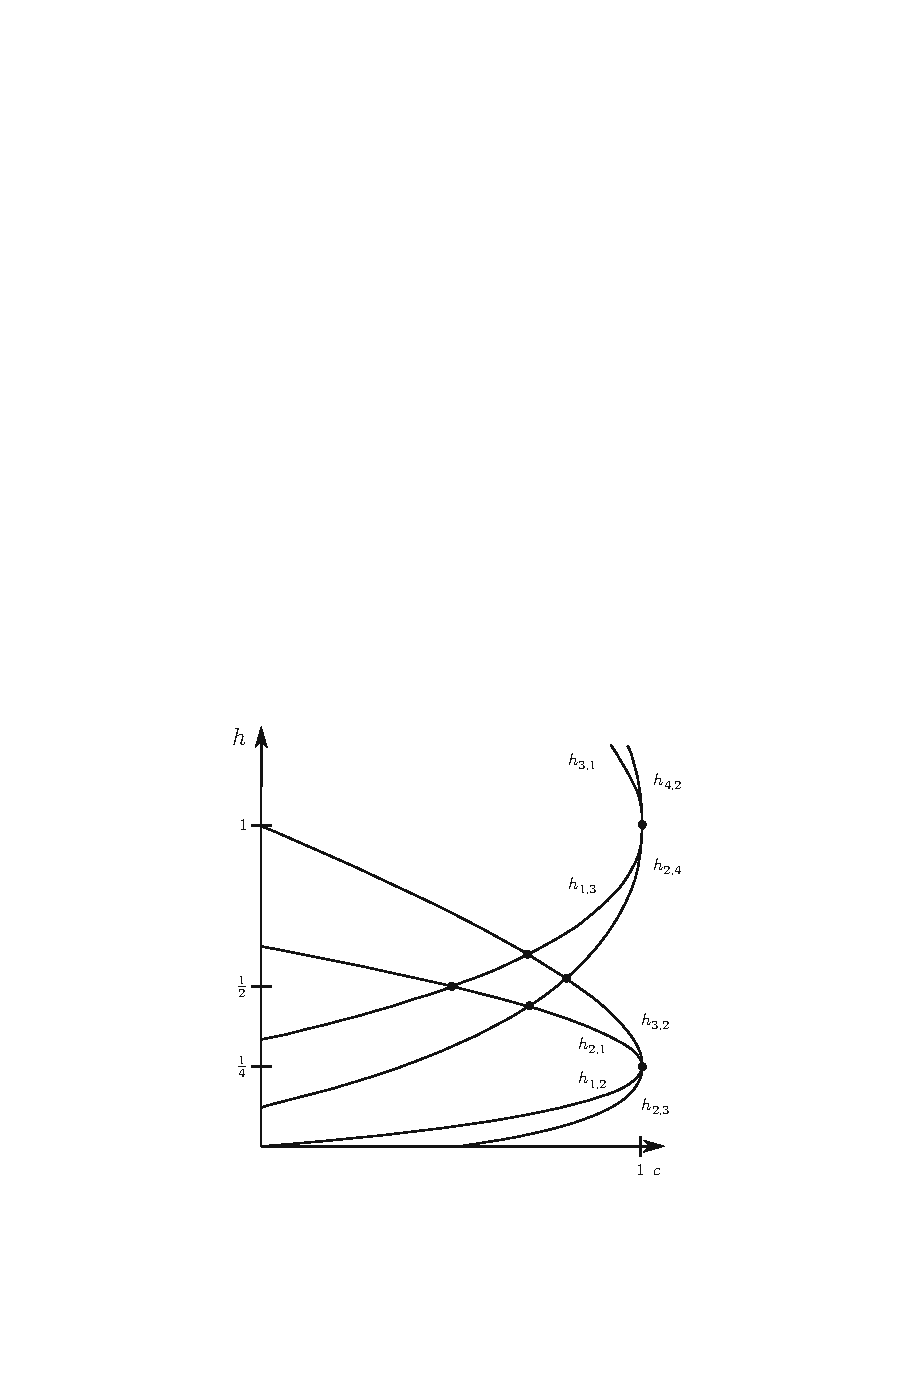
\includegraphics{figs/fig16.pdf}
	\label{unitary}
	\caption{Ka\v{c}行列式零点和中心荷之间的关系}
\end{figure}
\begin{itemize}
	\item $c>1,h> 0$:Ka\v{c}行列式无零点且其本征值都是正的,这个时候理论总是幺正
	\item $c=1$:Ka\v{c}行列式零点分布为$h=\frac{n^2}{4},n\in\mathbb{Z}$
	\item $c<1,h\geq 0$:只有图\ref{unitary}的交点处才会出现幺正表示
\end{itemize}
下面的定理给出了交点处的坐标:
\begin{theorem}[Unitary Minimal Models]
	$c<1,h\geq 0$的CFT,只有在中心荷满足:
	\begin{equation}
	\boxed{
			c=1-\frac6{m(m+1)}\quad m=3,4,\ldots
	}
	\end{equation}
	时才有幺正谱,谱为:
	\begin{equation}
		\boxed{
			h_{p,q}(m)=\frac{\left(\left(m+1\right)p-mq\right)^2-1}{4m\left(m+1\right)},\quad 1\leq p\leq m-1\mathrm{~and~}1\leq q\leq m
		}
	\end{equation}
\end{theorem}
我们原先说CFT的谱是无穷多或者连续的,但对于对称性只有Virasoro的CFT,幺正性直接让理论的谱变成有限离散的。这时的CFT我们称为\textbf{unitary minimal models}。有些时候理论不必是幺正的,不过我们还是希望这个CFT的谱依旧被限制为有限离散谱,这时的CFT称为\textbf{Minimal models},由下面的中心荷和谱定义:
\begin{theorem}[Minimal models]
	\begin{equation}
		\boxed{
			\begin{gathered}
				c=1-6\frac{(p-q)^2}{pq},\quad p,q\geq2,\quad p\perp q\\
			h_{r,s}(p,q)=\frac{(pr-qs)^2-(p-q)^2}{4pq},\quad 1\leq r\leq q-1\text{ and }1\leq s\leq p-1
			\end{gathered}
		}
	\end{equation}
\end{theorem}
类似这种谱有限离散,而且这时$h$还都是有理数的CFT我们称为\textbf{有理CFT(RCFT)}。
\begin{example}
	考虑$m=3$的幺正极小模型,这实际上是Ising Model二阶相变临界点处的理论,根据公式可以计算出中心荷为$\frac{1}{2}$,谱为:
	\begin{table}[H]
		\centering
		\renewcommand{\arraystretch}{1.5}
			\begin{tabular}{|c|c|}
				\hline
				$\frac{1}{2}$  & 0              \\ \hline
				$\frac{1}{16}$ & $\frac{1}{16}$ \\ \hline
				0              & $\frac{1}{2}$  \\ \hline
			\end{tabular}
		\caption{Ising模型的谱,横轴表示$1\leq p\leq 2$,纵轴表示$1\leq q\leq 3$}
	\end{table}
	从$p,q$取值范围来看似乎有$m(m-1)$个谱,但实际上有一半是重复的,只有$\mathrm{C}^2_m$个谱。
\end{example}

\section{Fusion Rules}
让我们从一个例子出发,利用\ref{33.31}
\begin{equation}
	\widehat{L}_{-2}\left.\phi(z)-\frac3{2\left(2h+1\right)}\widehat{L}_{-1}^2\right.\phi(z)=\left(\mathcal{L}_{-2}-\frac3{2\left(2h+1\right)}\mathcal{L}_{-1}^2\right)\left\langle\phi(w)\left.\phi_1(w_1)\ldots\phi_N(w_N)\right\rangle\right. =0
\end{equation}
得到微分方程:
\begin{equation}\label{37.2}
	\boxed{
		\left(\sum_{i=1}^N\left(\frac{h_i}{(w_i-w)^2}-\frac{1}{w_i-w}\partial_{w_i}\right)-\frac{3}{2(2h+1)}\partial_w^2\right)\left\langle\phi(w)\phi_1(w_1)\ldots\phi_N(w_N)\right\rangle=0
	}
\end{equation}
前面用共形对称性已经确定两点和三点函数只差一个常数系数,带入到方程中发现第一个non-trival的结果来自于三点函数:
\begin{equation}
	2\left(2h+1\right)\left(h+2h_2-h_1\right)=3\left(h-h_1+h_2\right)\left(h-h_1+h_2+1\right)
\end{equation}
$h,h_1,h_2$分别是$\phi,\phi_1,\phi_2$对应的共形权。这对三点函数的$C_{\phi\phi_1\phi_2}$做出了更强的限制,告诉我们绝大部分都是0。当然这个限制仅限于$h=h_{2,1}(m) \text{ or } h_{1,2}(m)$,这时上面的推导才成立,但是$h_1,h_2$是一般的。不妨取$h=h_{2,1}$,并把$h_1$也取为存在Null State的谱$h_{p,q}$,根据上面的方程可以解出不为0的条件是:
\begin{equation}
	h_2=\frac16+\frac h3+h_1\pm\frac23\sqrt{h^2+3hh_1-\frac12h+\frac32h_1+\frac1{16}}\in\{h_{p-1,q}(m),h_{p+1,q}(m)\}
\end{equation}
由OPE的一般表达式我们知道OPE是由一系列初级场和其导数,或者说次级场组合而成的,由于OPE有结合律,所以三点函数的计算可以看作是前两个先插入OPE\sn{我们假设第三个场隔得比较远,使得OPE的插入是精确的},然后和第三个场做两点函数,而两点函数不为零当且仅当共形权一致。上面的方程告诉我们三点函数不为零的条件是$h_2$只能取特定的两个值,从OPE去看这正说明了前两个场的OPE最终出来的那些场只能是共形权为$\{h_{p-1,q}(m),h_{p+1,q}(m)\}$的场的线性组合!这一思想完全可以推广到次级场的OPE:
\begin{equation}
	\begin{bmatrix}\phi_{(2,1)}\end{bmatrix}\times\begin{bmatrix}\phi_{(p,q)}\end{bmatrix}=\begin{bmatrix}\phi_{(p+1,q)}\end{bmatrix}+\begin{bmatrix}\phi_{(p-1,q)}\end{bmatrix}
\end{equation}
也就是说,$\phi_{(2,1)}$和$\phi_{(p,q)}$ Conformal family中的元素做OPE,最终得到的只能是$\phi_{(p-1,q)}$和$\phi_{(p+1,q)}$ Conformal family中元素的组合。
\begin{theorem}[Fusion rules of unitary minimal models]
	\begin{equation}
		\boxed{
			\left[\phi_{(p_1,q_1)}\right]\times \left[\phi_{(p_2,q_2)}\right]=\sum^{p_1+p_2-1}_{\begin{subarray}{l}
					k=1+|p_1-p_2|\\k+p_1+p_2\mathrm{~} \text{odd}\end{subarray}}\sum^{q_1+q_2-1}_{\begin{subarray}{l}
					l=1+|q_1-q_2|\\l+q_1+q_2\mathrm{~} \text{odd}\end{subarray}}\left[\phi_{(k,l)}\right]
		}
	\end{equation}
\end{theorem}
只要是RCFT,谱是离散有限的,都可以构造类似的融合规则:
\begin{equation}
	\boxed{
		[\left.\phi_i\right.]\times[\left.\phi_j\right.]=\sum_kN_{ij}^k\left[\left.\phi_k\right.\right],\quad N_{ij}^k\in\mathbb{Z}^+_0
	}
\end{equation}
根据OPE的性质可以知道这是一个交换代数,还是一个结合代数,其中的恒等元$[1]$就是Verma Module,对应真空表示,毕竟本身某个初级态的次级态就是用$N(T\cdots)$定义出来的。
\begin{theorem}
	\begin{equation}
		\boxed{
			\sum_lN_{kj}^lN_{il}^m=\sum_lN_{ij}^lN_{lk}^m
		}
	\end{equation}
	定义$(\overline{N}_i)_{jk}\equiv N_{ij}^k$,上式可以写成矩阵形式:
	\begin{equation}
		\boxed{
			\overline{N}_i\overline{N}_k=\overline{N}_k\overline{N}_i
		}
	\end{equation}
\end{theorem}
\begin{proof}
	证明就是使用交换律和结合律:
	\begin{equation}
		\begin{aligned}&\left[\phi_i\right]\times\left(\left[\phi_j\right]\times\left[\phi_k\right]\right)=\left[\phi_i\right]\times\sum_{l}N_{jk}^{l}\left[\phi_l\right]=\sum_{l,m}N_{jk}^{l}N_{il}^{m}\left[\phi_m\right]\\&\left(\left[\phi_i\right]\times\left[\phi_j\right]\right)\times\left[\phi_k\right]=\sum_{l,m}N_{ij}^{l}N_{lk}^{l}\left[\phi_m\right],\end{aligned}
	\end{equation}
\end{proof}
\subsection{Ising Model}

\section{Ka\v{c}\mbox{–}Moody Symmetry}
从现在开始,我们来考虑比Virasoro对称性更大的对称性。本节大量涉及无穷维李代数的艰深数学内容,大黄书专门用了两章进行铺垫介绍,这里不追求数学上的严谨性。\sn{数学读物可见\cite{Fuchs:1997af,Kac:1990gs}}
\subsection{Ka\v{c}\mbox{–}Moody Algebras}
Ka\v{c}\mbox{–}Moody对称性是理论中加入了其他守恒流,这些守恒流的洛朗模之间满足下面的代数关系:
\begin{definition}[Ka\v{c}\mbox{–}Moody Algebras]
	\begin{equation}\label{38.1}
		\boxed{
			\left[j_m^a,j_n^b\right]=i\sum_cf^{abc}j_{m+n}^c+k m\delta^{ab}\delta_{m+n,0}
		}
	\end{equation}
	$k$称为这个代数的level。
\end{definition}
从上面的定义看到$\{j_0^a\}$构成了上面这个代数的子代数,没有中心荷:
\begin{equation}\label{38.2}
	\left[j_0^a,j_0^b\right]=i\sum_cf^{abc}j_0^c
\end{equation}
这就是我们熟悉的李代数结构$\mathfrak{g}$,而Ka\v{c}\mbox{–}Moody代数可以看作是这个子代数的仿射化,记为$\hat{\mathfrak{g}}_k$。比如\ref{35.37}就是一个$\widehat{\mathfrak{su}}(2)_{1}$的代数结构。
\begin{theorem}[OPEs of Currents]
	由于OPE和对易关系蕴含完全相同的信息,所以前面的对易关系也可以翻译为流之间的OPE:
	\begin{equation}\label{38.3}
		\boxed{
			j^a(z)j^b(w)=\frac {k\delta^{ab}}{(z-w)^2}+\sum_c\frac{if^{abc}}{z-w}~j^c(w)+\cdots 
		}
	\end{equation}
\end{theorem}

\subsection{Sugawara Construction}
构造CFT首先要给出理论的谱,这可以通过寻找Ka\v{c}\mbox{–}Moody代数的表示得到,这个后面再说。理论在无穷小共形变换时的性质完全由能动张量刻画,本节的目的就是完全从自洽性出发把能动张量构造出来。

这些流是守恒流,就像我们构造Casimir算符一样,可以做下面的ansatz:
\begin{equation}
	T(z)=\gamma\sum_{a=1}^{\dim\mathfrak{g}}N\bigl(j^aj^a\bigr)(z)
\end{equation}
把所有的流加起来使得其再对称群变换下是不变的,现在根据$j^a$的共形权为$1$定出前面的归一化系数。
\begin{equation}
	L_m=\gamma\sum_{a=1}^{\dim\mathfrak{g}}\left(\sum_{l\leq-1}j_l^aj_{m-l}^a+\sum_{l>-1}j_{m-l}^aj_l^a\right)
\end{equation}
计算对易关系\footnote{计算中第四个等号利用了结构张量前两个指标反对称所导出的:
\begin{equation*}
	\begin{aligned}\sum_{l\leq-1}\left(j_l^bj_{m+n-l}^c-j_{l+n}^bj_{m-l}^c\right)&=\sum_{l\leq-1}j_l^bj_{m+n-l}^c-\sum_{l\leq-1+n}j_l^bj_{m+n-l}^c=-\sum_{l=0}^{n-1}j_l^bj_{m+n-l}^c\\\sum_{l>-1}\left(j_{m+n-l}^cj_l^b-j_{m-l}^cj_{l+n}^b\right)&=\sum_{l>-1}j_{m+n-l}^cj_l^b-\sum_{l>-1+n}j_{m+n-l}^cj_l^b=+\sum_{l=0}^{n-1}j_{m+n-l}^cj_l^b\end{aligned}
	\end{equation*}}:\sn{你依旧可以用OPE做}
\begin{align*}
		&[L_m,j_n^a]\\
		=&\gamma\sum_b\left(\sum_{l\leq-1}\left[j_l^bj_{m-l}^b,j_n^a\right]+\sum_{l>-1}\left[j_{m-l}^bj_l^b,j_n^a\right]\right) \\
		=&\gamma\sum_b\left(\sum_{l\leq-1}\left(j_l^b\bigl[j_{m-l}^b,j_n^a\bigr]+\bigl[j_l^b,j_n^a\bigr]j_{m-l}^b\right)+\sum_{l>-1}\left(j_{m-l}^b\bigl[j_l^b,j_n^a\bigr]+\bigl[j_{m-l}^b,j_n^a\bigr]j_l^b\right)\right) \\
		=&-2\gamma nkj_{m+n}^{a}+\gamma\sum_{b,c}if^{bac}\sum_{l\leq-1}\big(j_{l}^{b}j_{m+n-l}^{c}+j_{l+n}^{c}j_{m-l}^{b}\big) \\
		&+\gamma\sum_{b,c}if^{bac}\sum_{l>-1}\bigl(j_{m+n-l}^{c}j_{l}^{b}+j_{m-l}^{b}j_{l+n}^{c}\bigr)\displaybreak\\%换页
		=&-2\gamma nkj_{m+n}^a-\gamma\sum_{b,c}if^{bac}\sum_{l=0}^{n-1}[j_l^b,j_{m+n-l}^c] \\
		=&-2\gamma nkj_{m+n}^a-\gamma\sum_{b,c}if^{bac}\sum_{l=0}^{n-1}\sum_dif^{bcd}j_{m+n}^d \\
		=&-2\gamma nkj_{m+n}^a+\gamma n\sum_{b,c,d}f^{bac}f^{bcd}j_{m+n}^d. 
\end{align*}
李代数的伴随表示有下面的等式:
\begin{equation}\label{38.6}
	\sum_{b,c}f^{bac}f^{bcd}=-2C_{\mathfrak{g}}\delta^{ad}
\end{equation}
其中$C_{\mathfrak{g}}$叫\textbf{dual Coxeter number},下表给出了一些李群的dual Coxeter number:
\begin{table}[H]
	\centering
	\begin{tabular}{|c|c|c|c|c|c|}
		\hline
		Algebar        & $A_n$ & $D_n$  & $E_6$ & $E_7$ & $E_8$ \\ \hline
		$C_{\mathfrak{g}}$ & $n+1$ & $2n-2$ & $12$  & $18$  & $30$  \\ \hline
	\end{tabular}
	\caption{ADE分类的Coxeter number,在现在的语境下可以将$A_n$对应$\mathfrak{su}_{n+1}$,$D_n$对应$\mathfrak{so}_{2n}$}
\end{table}
\begin{theorem}[Sugawara energy–momentum tensor]
	$\hat{\mathfrak{g}}_k$所确定CFT的能动张量由下式给定:
	\begin{equation}\label{38.7}
		\boxed{
			T(z)=\frac1{2\left(k+C_{\mathfrak{g}}\right)}\sum_{a=1}^{\dim\mathfrak{g}}N\left(j^aj^a\right)(z)
		}
	\end{equation}
\end{theorem}
利用能动张量OPE或者$\frac c2=\left\langle0\right|L_{+2}L_{-2}\left|0\right\rangle $可计算出理论的中心荷:
\begin{theorem}
	Sugawara构造出来的CFT中心荷为:
	\begin{equation}
		\boxed{
			c=\frac{k\dim\mathfrak{g}}{k+C_{\mathfrak{g}}}
		}
	\end{equation}
\end{theorem}
\subsection{WZNW Models}
前面导出能动张量的过程再次强调了研究CFT时很多情况下拉氏量是放在次要位置的,我们当然也可以直接构造一个有流对称代数的拉氏量,即所谓的WZW模型,然后再用作用量变分导数得到能动张量。本节目的是知道这样做有多麻烦。

从自由玻色场来看,其作用量可以写成下面的形式:\sn{已重新选取耦合常数}
\begin{equation}
	\mathcal{S}=\frac1{8\pi}\int_\Sigma\mathrm{d}^2x\partial^\mu g^{-1}\partial_\mu g=\frac1{8\pi}\int_\Sigma\mathrm{d}^2x\partial g^{-1}\overline{\partial}g
\end{equation}
这里$\Sigma$是复平面这个最简单的黎曼曲面,其中$g$是:
\begin{equation}
	g:\mathbb{C}\to\mathcal{U}(1);z\mapsto g(z,\overline{z})=\exp(i\varphi(z,\overline{z}))
\end{equation}
前面说$\phi\mapsto\phi+a$是$U(1)$对称性或许还有些困惑,从这个作用量就很好看出来的确是$g\mapsto e^{ia} g$的$U(1)$变换,WZNW模型就是对这个模型的非阿贝尔推广。
\subsubsection{Nonlinear Sigma Models}
\begin{definition}
	非线性sigma模型包含一个定义在某个黎曼曲面上的到群流形的玻色场$g:\Sigma\to G$\footnote{或者精确点说是在$G$的幺正表示里面取值},作用量为:
	\begin{equation}
		\mathcal{S}_0=\frac1{2a^2}\int_\Sigma\mathrm{d}^2x\mathrm{~Tr}\left(\partial^\mu g^{-1}\partial_\mu g\right)
	\end{equation}
	这个$\mathrm{Tr}$其实要写成$\mathrm{Tr^\prime}$和一般的取迹进行区分,如果在某个表示下,生成元矩阵有$\mathrm{Tr}(t^a t^b)=x\delta^{ab}$,那么$\mathrm{Tr^\prime}\equiv\frac{1}{x}\mathrm{Tr}$。后面假设都已经做了这个归一化。
\end{definition}
对作用量进行变分得到运动方程:
\begin{equation}
	\partial^\mu(g^{-1}\partial_\mu g)=0
\end{equation}
这直接说明了存在下面的守恒流:
\begin{equation}
	J_\mu=g^{-1}\partial_\mu g
\end{equation}
这个守恒流对应模型的global $G\times G$对称性。黎曼曲面是一个一维复流形,任何一点领域都同胚于复平面的开子集,所以可以在上面local地赋予复坐标,定义上面守恒流的全纯和反全纯部分:
\begin{equation}
	J_z=g^{-1}\partial g,\quad\bar{J}_{\overline{z}}=g^{-1}\overline{\partial}g\Rightarrow\partial\bar{J}_{\overline{z}}+\bar{\partial}J_z=0
\end{equation}
一般而言,全纯和反全纯部分不能单独守恒,和$U(1)$的情况不一样,我们期望在理论中加上一些项,让对称性进一步扩大为反全纯和全纯部分单独守恒。
\begin{definition}[Wess-Zumino term]
	\begin{equation}
		\Gamma=\frac{-i}{12\pi}\int_B\mathrm{d}^3y\epsilon_{\alpha\beta\gamma}\operatorname{Tr}\left(\widetilde{g}^{-1}\partial^\alpha\widetilde{g}\widetilde{g}^{-1}\partial^\beta\widetilde{g}\widetilde{g}^{-1}\partial^\gamma\widetilde{g}\right)
	\end{equation}
	这里$B$是一个带边三维流行,其边界为$\Sigma$,$\tilde{g}: B\to G$可看作是$g$从Boundary到Bulk的扩张,这种扩张不是唯一的,流形$B$也不是唯一的。但可以证明这个差别只会体现为$2n\pi i$,所以虽然作用量上面看不一样,但是最终就欧几里得路径积分而言$e^{-\Gamma}$是唯一的,所以不会对场论造成任何影响。
\end{definition}
\subsubsection{Wess-Zumino-Novikov-Witten Models}
考虑下面的作用量:
\begin{equation}
	\mathcal{S}=\mathcal{S}_0+k\Gamma,\quad k\in\mathbb{Z}
\end{equation}
按照前面说的虽然$\Gamma$不唯一,但是理论唯一。计算运动方程为:
\begin{equation}
	\partial^\mu(g^{-1}\partial_\mu g)+\frac{a^2ik}{4\pi}\epsilon_{\mu\nu}\partial^\mu(g^{-1}\partial^\nu g)=0
\end{equation}
在复坐标下为:
\begin{equation}
	\left(1+\frac{a^2k}{4\pi}\right)\partial(g^{-1}\overline{\partial}g)+\left(1-\frac{a^2k}{4\pi}\right)\overline{\partial}(g^{-1}\partial g)=0
\end{equation}
所以为了让流的全纯和反全纯部分的流单独守恒,要求:
\begin{equation}
	a^2=4\pi/k
\end{equation}
\begin{theorem}[$\widehat{\mathfrak{g}}_k$ WZNW Models]
	\begin{equation}
		\mathcal{S}=\frac k{8\pi}\int_\Sigma\mathrm{d}^2x\mathrm{~Tr}\left(\partial^\mu g^{-1}\partial_\mu g\right)+k\Gamma ,\quad k\in\mathbb{Z}^+
	\end{equation}
\end{theorem}
另外一个$a^2=-4\pi/k$的解并不是我们关注的流守恒。左右流的单独守恒体现到场上是场可以分解为$g(z,\overline{z})=g_L(z)g_R(\overline{z})$,提现到体系的对称群上是从global $G\times G$扩张为local的$G(z)\times  G(\bar z)$,即下面的变换下作用量不变:
\begin{equation}
	g(z,\bar{z})\to\Omega(z)g(z,\bar{z})\overline{\Omega}^{-1}(\bar{z}),\quad \Omega(z),\bar \Omega(\bar z)\in G
\end{equation}
rescale守恒流:
\begin{equation}
	\begin{aligned}
		{J(z)} &\equiv-\frac k2J_z(z)=-\frac k2\partial gg^{-1} \\
	\bar{J}(\overline{z}) &\equiv\frac k2\bar{J}_{\overline{z}}(\overline{z})=\frac k2g^{-1}\overline{\partial}g
	\end{aligned}
\end{equation}
然后类似于YM理论里面的操作,在生成元$t^a$上投影,$J=J^at^a$,可以证明$J^a$就是那些Ka\v{c}\mbox{-}Moody流,理论的能动张量也就是Sugawara构造的那样!

\subsection{Knizhnik\mbox{–}Zamolodchikov Equation}
前面我们研究初级场实际上都是在看其在Virasoro代数下如何变换,现在显然我们要找更大对称群的表示。就像是YM理论一样,除了Lorentz变换本身对场进行了分类,分成标量场,矢量场等等。然后理论中本身冒出来一个规范对称群,要求理论中不同的场$\phi_a$之间在$\phi_a\to U^{ab}_R\phi_b$的规范变换下理论仍不变。这种场之间的内在对称性实际上就类似于Ka\v{c}\mbox{-}Moody对称性,场除了被Virasoro表示分类(不同的共形权),还要在流代数的表示之中。
\begin{definition}[Ka\v{c}\mbox{–}Moody (chiral) primary field]
	\begin{equation}\label{kac}
		\boxed{
			j^a(z)\phi_R^r(w)=\frac1{z-w}\sum_s\left(t_R^a\right)_s^r\phi_R^s(w)+\cdots 
		}
	\end{equation}
	$j^a$是生成变换群$G$的流,$R$表示$\{\phi_R^a\}$具体处于群的哪个表示,$t^a_R$是生成元的表示矩阵。满足这一条件的初级场,一定也是Virasoro初级场,你可以尝试去计算Sugawara能动张量和$\phi$之间的OPE来证明这一点。
\end{definition}
\begin{remark}
	本节我们只考虑全纯部分,因为全纯反全纯完全解耦,把反全纯部分也加上来后初级场定义为:
	\begin{equation}
		\begin{aligned}&j^a(z)\phi_{R,\bar R}(w,\bar{w})\sim\frac{t_R^a\phi_{R,\bar R}(w,\bar{w})}{z-w}\\&\bar{j}^a(\bar{z})\phi_{R,\bar R}(w,\bar{w})\sim-\frac{\phi_{R,\bar R}(w,\bar{w})t_{{\bar R}}^a}{\bar{z}-\bar{w}}\end{aligned}
	\end{equation}
	$R,\bar R$分别表示全纯和反全纯部分处于哪个表示。另外,不少文献对\ref{kac}的定义差个负号,这会导致后面的方程正负号有些差别,但这无伤大雅。
\end{remark}
\subsection{Ward Identity for Ka\v{c}\mbox{–}Moody Symmetries}
Virasoro初级场有Ward恒等式限制它们之间的关联函数形式,同样这里也有更强的限制:
\begin{theorem}
	\begin{equation}\label{38.11}
		\boxed{
			\begin{aligned}
				\left<j^{a}(z)\phi_{R_{1}}(w_{1},\overline{w}_{1})\right.& \ldots\phi_{R_N}(w_N,\overline{w}_N)\rangle   \\
				&=\sum_{i=1}^N\frac{t_{R_i}^a}{z-w_i}\left\langle\left.\phi_{R_1}(w_1,\overline{w}_1)\ldots\phi_{R_N}(w_N,\overline{w}_N)\right.\right\rangle +\text{regular}
			\end{aligned}
		}
	\end{equation}
	这里$\{\phi_{R_i}\}$是Ka\v{c}\mbox{–}Moody (chiral) primary field,$t_{R_i}$仅仅作用于$\phi_{R_i}$,它们的矩阵指标没有明写出来。
\end{theorem}
\begin{proof}
	证明过程和共形Ward恒等式的证明一模一样,守恒流给出守恒荷从而给出Ka\v{c}\mbox{-}Moody代数作用下场的无穷小变换的形式:
	\begin{equation}
		-\delta_\epsilon\phi(w)=\oint_{\mathcal{C}(w)}\frac{dz}{2\pi i}\sum_a\left.j^a(z)\right.\epsilon^a(z)\phi(w)
	\end{equation}
	考虑关联函数的无穷小变换:
	\begin{equation}
		\begin{aligned}
			&\delta_{\epsilon}\left\langle\phi_{R_{1}}(w_{1},\overline{w}_{1})\ldots\phi_{R_{N}}(w_{N},\overline{w}_{N})\right\rangle  \\
			&=\oint_{\mathcal{C}(w_1,...,w_N)}\frac{dz}{2\pi i}\sum_a\epsilon^a(z)\Big\langle j^a(z)\phi_{R_1}(w_1,\overline{w}_1)\ldots\phi_{R_N}(w_N,\overline{w}_N)\Big\rangle  \\
			&=\sum_{i=1}^N\oint_{\mathcal{C}(w_i)}\frac{dz}{2\pi i}\sum_a\epsilon^a(z)\big<\phi_{R_1}(w_1,\overline{w}_1)\ldots\bigg(j^a(z)\phi_{R_i}(w_i,\overline{w}_i)\bigg)\ldots\phi_{R_N}(w_N,\overline{w}_N)\big>\\
			&=\sum_{i=1}^N\oint_{\mathcal{C}(w_i)}\frac{dz}{2\pi i}\sum_a\epsilon^a(z)\frac{t_{R_i}^a}{z-w_i}\left\langle\phi_{R_1}(w_1,\overline{w}_1)\ldots\phi_{R_N}(w_N,\overline{w}_N)\right\rangle
		\end{aligned}
	\end{equation}
	比较第一个等号和最后一个等号即得证。由于上面的关联函数在$G$的global作用下实际上要不变,所以上面这一长串等式,\textbf{在$\epsilon$为常数时},实际上为0,所以我们其实还有下面的等式成立:\footnote{证明的前一半是local形式的证明,因为证明中群变换的参数$\epsilon$是local的,所以才能说积分号里面的东西相等;证明global的形式实际上是让$\epsilon$是global的参数,也就是考虑global的群变换,这部分才是对称性,由于$\epsilon$与$z$无关,所以上式最后一个等式可以把围道积分积出来得到下式。\ref{31.37}也可以用这种方式来看。}
	\begin{equation}
		\boxed{
			\sum_{i=1}^nt_i^a\left<\phi_1(z_1)\cdots\phi_n(z_n)\right>=0
		}
	\end{equation}
	这个等式类似于\ref{31.37},确定了两点和三点函数。
\end{proof}
\subsection{Ka\v{c}\mbox{–}Moody descendant fields}
从态的角度看,现在对称性增大了,原先构造descendant fields是用Virasoro初级场配合$L_{-n},n\geq 1$去构造,现在初级场应该用Ka\v{c}\mbox{–}Moody初级场,产生算符应该用对称性所对应的$j_{-n},n\geq 1$\footnote{现在估计就不难从数学上去理解我们为什么构造Free Bosons的希尔伯特空间的时候是用$j_{-n}$去构造了,因为理论是$\hat{\mathfrak{u}}(1)$的对称性,所以我们希望初级场是Ka\v{c}\mbox{-}Moody的,次级态也是,所以$j_{-n}$作用真空上去得到Verma模,作用到顶点算符构造的初级场上面得到次级态($jV_\alpha$的OPE确实有\ref{kac}的形式,$U(1)$还是过于trivial,生成元表示就是一个常数。)。由于$T$就是用$j$ Sugawara构造来的,所以也同时是Virasoro初级态。}。\sn{下面的$\mathcal{U}(\hat{g}_k)$不少文献称为$\hat{g}_k$的泛包络代数的表示,名字很唬人,简单点说就是那些$j^a_{-n}$构成的一个结合代数,也就是$j^a_{-n}j^b_{-m}\ldots$,下标$+$表示只取$n\geq 1$。}
\[\text{Ka\v{c}\mbox{–}Moody descendant fields} = \{\mathcal{U}(\hat{g}_k)_+\ket{\phi_R}\}\]
同样类似\ref{eq:33.30}态算符对应给出次级场:
\begin{equation}
	\boxed{
		(\widehat{j}_{-n}^a\phi_R)(w)=\oint_{\mathcal{C}(w)}\frac{dz}{2\pi i}\frac1{(z-w)^n}j^a(z)\phi_R(w)
	}
\end{equation}
\begin{example}
	\begin{equation}
		\begin{aligned}
			j_0^a\left|\phi_R\right\rangle & =\lim\limits_{w\to0}\oint\frac{dz}{2\pi i}j^{a}(z)\phi_{R}(w)\big|0\big>  \\
			&=\lim_{w\to0}\oint\frac{dz}{2\pi i}\left(\frac1{z-w}t_R^a\phi_R(w)+\cdots\right)\left|0\right\rangle=t_R^a\left|\phi_R\right\rangle 
		\end{aligned}
	\end{equation}
	这个方程蛮重要的,它告诉我们$\phi_R$生成了$j_0$的表示空间而$j_0$就是没有仿射化的,通常的李代数\ref{38.2}的群表示,一下就看清楚了$\phi_R$这个下标$R$的具体意义。而对称性变大之后,最高权除了由$L_0$本征值$h$标记,还应该由$j_0^a$所处的表示来标记,后面用例子来感受这一点。
\end{example}
利用这个我们可以类似去计算Ka\v{c}\mbox{–}Moody descendant fields和Ka\v{c}\mbox{–}Moody primary fields之间的关联函数,有与\ref{33.31}类似的方程:
\begin{theorem}
	\begin{equation}\label{38.15}
		\boxed{
			\begin{gathered}
				\left\langle\widehat{j}_{-n}\phi_R(w)\phi_{R_1}(w_{1})\ldots\phi_{R_N}(w_{N})\right\rangle=\mathcal{J}_{-n}\langle\phi_R(w)\phi_{R_1}(w_{1})\ldots\phi_{R_N}(w_{N})\rangle  \\
				\text{Where,}\qquad\mathcal{J}_{-n}=-\sum_{i=1}^N\frac{t^a_{R_i}}{(w_i-w)^n}
			\end{gathered}
		}
	\end{equation}
\end{theorem}

更关键的是去找理论中的零模,从而得到类似\ref{37.2}的对初级场关联函数约束。
\begin{theorem}[Knizhnik–Zamolodchikov Equation]
	\begin{equation}\label{KZ}
		\boxed{
			\left(\partial_{w_i}-\frac{1}{k+C_{\mathfrak{g}}}\sum_{j\neq i}\left.\frac{\sum_{a}t_{R_i}^{a}\otimes t_{R_j}^{a}}{w_i-w_j}\right)\big\langle\phi_{R_1}(w_1)\ldots\phi_{R_N}(w_N)\big\rangle=0\right.
		}
	\end{equation}
	上式省略了矩阵下标,$t^a_{R_i}$只作用于$\phi_{R_i}$。上面方程对任意的$i=1,\ldots,N$都成立。
\end{theorem}
\begin{proof}
	\begin{equation}
		\begin{aligned}
			L_{-1}\left|\phi_{R}^{r}\right\rangle & =\frac1{2\left(k+C_{\mathfrak{g}}\right)}\sum_a\left(\sum_{l\leq-1}j_l^aj_{-1-l}^a+\sum_{l>-1}j_{-1-l}^aj_l^a\right)\ket{\phi_R^r}  \\
			&=\frac1{2\left(k+C_{\mathfrak{g}}\right)}\sum_a\left(j_{-1}^aj_0^a+j_{-1}^a j_0^a\right)\ket{\phi_R^r}\\
			&=\frac1{k+C_{\mathfrak{g}}}\sum_aj_{-1}^a\sum_s{\left(t_R^a\right)^r}_s\ket{\phi_R^r},
		\end{aligned}
	\end{equation}
	直接给出了一个Null State:
	\begin{equation}
		\left(\widehat{L}_{-1}-\frac1{k+C_{\mathfrak{g}}}\sum_a\widehat{j}_{-1}^at_R^a\right)\phi_R(z)=0
	\end{equation}
	这可以看作是Sugawara构造用次级态表述。把它插在关联函数中恒为0:
	\begin{equation}
		0=\left\langle\phi_{R_1}(w_1)\ldots\left(\widehat{L}_{-1}-\frac1{k+C_{\mathfrak{g}}}\sum_a\widehat{j}_{-1}^at_{R_i}^a\right)\phi_{R_i}(w_i)\ldots\phi_{R_N}(w_N)\right\rangle 
	\end{equation}
	再利用\ref{33.31}和\ref{38.15}即可证明。
\end{proof}
注意这个约束非常一般,前面\ref{37.2}好歹还要求$\ket{h}$本身就是有零模的谱,对$h$有约束,这里就啥也没有了。KZ方程的解催生出了非常多的数学问题,由于四点函数不能被共形对称性很好的确定,所以我们比较关心这个方程能否给出四点函数的形式?文章\cite{Knizhnik:1984nr}在末尾用合流超几何函数给了答案。
\begin{remark}
	本节前面的讨论相当于选取了一个特殊的基底,\ref{38.6}更一般的表述是下面的Killing型:
	\begin{equation}
		K^{ab}=\frac1{2g}\operatorname{Tr}\left(\operatorname{ad}_{t^a}\operatorname{ad}_{t^b}\right)=\frac1{2g}f^{acd}f^{bdc}
	\end{equation}
	前面我们在$\mathfrak{g}$中shift基底将$K_{ab}$化为$\delta_{ab}$,\ref{38.1}、\ref{38.3}、\ref{38.7}和\ref{KZ}的形式都要发生相应的变化,具体来说就是$\delta^{ab}\to K_{ab}$,注意$J^aJ^a$中隐含了一个$\delta_{ab}$。
\end{remark}

\section{Example: Highest Weight Representations of $\widehat{\mathfrak{su}}(2)_{k}$ }
 $\widehat{\mathfrak{su}}(2)_{k}$流代数和我们熟悉的角动量系统非常接近,首先按照下面的方式构造出流中的上升下降算符:
 \begin{equation}
 	\hat{j}_m^3=\frac1{\sqrt{2}}~j_m^3~,\quad\quad\hat{j}_m^\pm=\frac1{\sqrt{2}}~\left(j_m^1\pm i~j_m^2\right)
 \end{equation}
满足对易关系:
\begin{equation}
	\left[\hat{j}_m^3,\hat{j}_n^3\right]=\frac{mk}2\delta_{m+n,0},\quad\left[\hat{j}_m^3,\hat{j}_n^\pm\right]=\pm\hat{j}_{m+n}^\pm,,\quad\left[\hat{j}_m^+,\hat{j}_n^-\right]=km\delta_{m+n,0}+2\hat{j}_{m+n}^3
\end{equation}
前面就提到过$\{j_0\}$生成无中心荷的$\mathfrak{su}(2)$子代数,而且不难看到$L_0$和他们是对易的,所以现在$L_0$的$h$模是简并的,简并态构成的子空间是$\mathfrak{su}(2)$子代数的表示空间,这个表示空间还不只有一个不等价不可约表示,可能是很多不等价不可约表示直和起来构造出的更大的空间。所以现在最高权应该有两个指标标记,一个指标是其共形权$h$,表示其能量$L_0$,最高的含义依旧是:
\begin{equation}
	L_0\ket{h}=h\ket{h,q},\quad L_n\ket{h,q}=0,\quad \forall n>0
\end{equation}
第二个标记$q$是在说其处于哪个$\mathfrak{su}(2)$的表示,$\mathfrak{su}(2)$群的表示可以用自旋$l=0,\frac{1}{2},1,\ldots$去标记,而我们这里关心的是最高权,所以它在$\mathfrak{su}(2)$的表示中也是最高的那个,也就是$m=l$,这里我们设$q=2l\in\mathbb{Z}^+_0$。另外它作为最高权还要类似$L_{-n}$湮灭一样被$j^a_{-n}$湮灭:
\begin{equation}
	\begin{aligned}\hat{j}_n^3\left|h,q\right\rangle&=\hat{j}_n^\pm\left|h,q\right\rangle=0\quad\text{for }n>0\\\hat{j}_0^3\left|h,q\right\rangle&=\frac{q}{2}\left|h,q\right\rangle,\\\hat{j}_0^+\left|h,q\right\rangle&=0.\end{aligned}
\end{equation}
这些条件合起来就定义了一个最高权表示,与Virasoro代数不同,初级态不止包含这些最高权,实际上它应该包含所有$h$模简并的态,或者说我们要用$\hat {j}_0^\pm$继续在$\mathfrak{su}(2)$的自旋$q/2$表示中升降把表示空间构造全:\sn{再次强调按照定义这些$\alpha\neq 0$的态不是最高权,它们在$\mathfrak{su}(2)$的表示下不是最高的。}
\begin{equation}
	\left|h,q_\alpha\right\rangle:=\left(\hat{j}_0^-\right)^\alpha\left|h,q\right\rangle ,\quad \alpha =0,1,2,\ldots,q
\end{equation}
这就对应于前面Ka\v{c}\mbox{-}Moody初级场的$\ket{h,q_\alpha}$,显然从这个构造就可以看出来$\ket{h,q_\alpha}$张成$\mathfrak{su}(2)$的一个表示。利用Sugawara构造得知:
\begin{equation}
	L_0=\frac1{2\left(k+2\right)}\sum_{a=1}^3\left(\sum_{l\leq-1}j_{+l}^aj_{-l}^a+\sum_{l>-1}j_{-l}^aj_{+l}^a\right)
\end{equation}
由此可计算$\ket{h,q}$关于$L_0$的本征值:
\begin{equation}
	\begin{aligned}
		L_{0}\left|h,q\right\rangle & =\frac1{2\left(k+2\right)}\sum_{a=1}^{3}j_{0}^{a}j_{0}^{a}\left|h,q\right\rangle   \\
		&=\frac1{k+2}\sum_{a=1}^3\hat{j}_0^a\hat{j}_0^a\left|h,q\right\rangle=\frac{q(q+2)}{4(k+2)}\left|h,q\right\rangle 
	\end{aligned}
\end{equation}
计算的最后利用了$j_0^aj_0^a$是$\mathfrak{su}(2)$的Casimir算符。但是我们又知道本征值应该为$h$,所以$L_0$的谱和允许的表示之间是有关联的,要求:
\begin{equation}
	\boxed{
		h=\frac{q(q+2)}{4(k+2)}
	}
\end{equation}
而$q\in\mathbb{Z}^+_0$,所以理论中的谱可取值被极大限制住了,这也再次说明了这个模型是个RCFT。上面做的这些实际上是在考虑$\widehat{\mathfrak{su}}(2)_k$的非常特殊的一个$\mathfrak{su}(2)$子群,其实这样的子群有无数多个$\mathfrak{su}(2)_{(n)}\subset\widehat{\mathfrak{su}}(2)_k$:\sn{\[\begin{aligned}
		&\left[L_0,\widetilde{j}^{\pm}_{(n)}\right]=\mp n\widetilde{j}^{\pm}_{(n)}\\
		&\left[\widehat{j}_0^3,\widetilde{j}^{\pm}_{(n)}\right]=\pm \widetilde{j}^{\pm}_{(n)}
	\end{aligned}\]
所以$h$的增加以1为单位,$q$的增加以2为单位}
\begin{equation}
	\boxed{
		\begin{aligned}
			&\widetilde{j}_{(n)}^+ =\frac1{\sqrt{2}}\left(j_{-n}^1+i~j_{-n}^2\right),  \\
			&\widetilde{j}_{(n)}^- =\frac1{\sqrt{2}}\left(j_{+n}^1-i~j_{+n}^2\right),  \\
			&\widetilde{j}_{(n)}^{3} =\frac1{\sqrt{2}}~j_0^3-\frac{n~k}2~, 
		\end{aligned}
	}
\end{equation}
首先考虑$\mathfrak{su}(2)_{(1)}$,计算$j^+_{(1)}\ket{h,q}$的模:
\begin{equation}
	\begin{aligned}
		\langle h,q\mid\tilde{j}^{-}_{(1)}\tilde{j}^{+}_{(1)}\big|h,q\big\rangle & =\langle h,q\mid\begin{bmatrix}\tilde{j}^-_{(1)},\tilde{j}^+_{(1)}\end{bmatrix}\big|h,q\big\rangle   \\
		&=\langle h,q\mid-2\tilde{j}^3\mid h,q\rangle  \\
		&=-2\bra{h,q}j_0^3-\frac k{2}\ket{h,q} \\
		&=-q+k
	\end{aligned}
\end{equation}
而我们如果考虑幺正表示,所有的谱模应当正定,所以$q\leq k$。
\begin{theorem}
	$\widehat{\mathfrak{su}}(2)_k$最高权表示幺正要求$\boxed{0\leq q\leq k}$。
\end{theorem}
我们只说明了必要性,请相信它也是充分的。现在考虑其他$\mathfrak{su}(2)_{(n)}$。现在考虑具体的$k=1$的简单情形,考虑$\ket{0,0}$这个最高权,反复作用$\widetilde{j}_{(n)}^\pm$去构造表示空间中的其它态,表示空间中的向量我们仍用本征值$h,q$标记,但是它们不是最高权,所以前面的一些约束都没有了。最高权表示对应的初级态$\ket{h,q_\alpha}$相对$\widetilde{\mathfrak{su}}(2)_{(0)}$处在自旋$q/2$表示中,自然想到把这些初级态作用$\widetilde{j}_{(n)}^\pm$之后应该是别的$\widetilde{\mathfrak{su}}(2)_{(n)}$子群的表示。

比如$\tilde{j}_{(1)}^3\ket{0,0}=-\frac{1}{2}\ket{0,0}$,而且$\tilde{j}_{(1)}^-\ket{0,0}=0$,所以$\{\ket{0,0},\tilde{j}_{(1)}^+\ket{0,0}=\ket{0,0}\}$处于$\widetilde{\mathfrak{su}}(2)_{(1)}$的自旋$1/2$表示,对应$(h,q)=\{(0,0),(1,2)\}$。

$\tilde{j}_{(2)}^3\tilde{j}_{(1)}^+|0,0\rangle =0$且$\tilde{j}_{(2)}^+\tilde{j}_{(1)}^+|0,0\rangle =0$,所以$\tilde{j}_{(1)}^+|0,0\rangle $又处在$\widetilde{\mathfrak{su}}(2)_{(2)}$的自旋$0$表示。$\{\tilde{j}_{(1)}^+|0,0\rangle ,\tilde{j}_{(3)}^{+}\tilde{j}_{(1)}^{+}|0,0\rangle \}$又张成$\mathfrak{su}(2)_{(3)}$的自旋$1/2$表示,对应$(h,q)=\{(0,0),(4,4)\}$。可见,由于这些不同$n$对应$\tilde{j}_{(n)}^\pm$的是不对易的,所以这些表示是以某种方式“纠缠”在一起的。这个过程可以无限进行下去,我们得到权图\ref{fig17}。
\begin{figure}
	\centering
	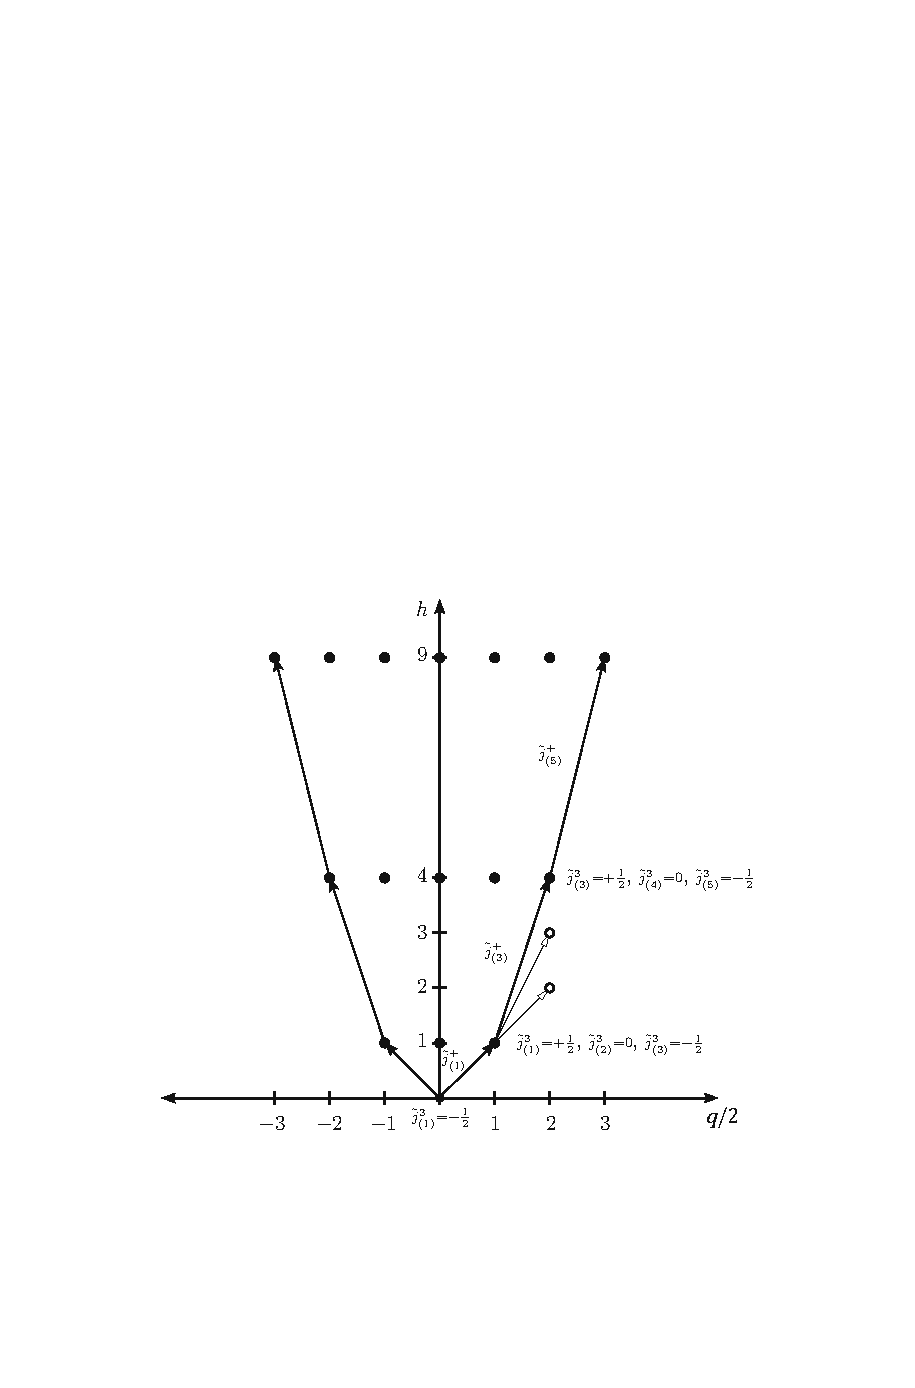
\includegraphics{figs/fig17.pdf}
	\caption{这些黑点表示作用$\widetilde{j}^\pm_{(n)}$可以得到的态,实心箭头表示用roots升降权,空心箭头表示作用任何一个root上去都得0}
	\label{fig17}
\end{figure}

这个权图是有边界的,边界为$(h,q)=(m^2,2m),m\in\mathbb{Z}$。这些边界才是真正要紧的,构造次级态就看它们,就$\widehat{\mathfrak{su}}(2)_1$而言,知道了边界的那些态,就足够构造整个希尔伯特空间,下面从玻色子的想法来说明。

玻色子体系是有$\widehat{\mathfrak{su}}(2)_1$代数的,具体而言可以由$R=\sqrt{2}$上的紧致化实现:\sn{后面的$(h,q)$表示场对应的态所对应的$L_0,\widehat{j}^3_0$本征值}
\begin{equation}
	\begin{aligned}j(z)&=i\partial X(z,\overline{z})&\left(h,q\right)&=\left(1,0\right),\\V_{\pm\sqrt{2}}&=:e^{\pm i\sqrt{2}X}:&\left(h,q\right)&=\left(1,\pm2\right)\end{aligned}
\end{equation}
前面提到过还应存在初级场:
\begin{equation}
	V_{\pm\sqrt{2}m}=:e^{\pm i\sqrt{2}mX}:\quad (h,q)=(m^2,\pm 2m)
\end{equation}
似乎这些场就能对应到权图上面的边界态,其实这是可以严格证明的。根据这一点,由玻色场希尔伯特空间$j_{-n}\ket{\alpha}$的启发,用边界态作用$j_{-n}$上去应该就能得到$\widehat{\mathfrak{su}}(2)_1$模型完整的$\ket{0,0}$最高权表示表示空间了。每个态上面的简并度也可以很方便地用生成函数表达为:\sn{$q^h$前面的系数表示$L_0$的本征值为$h$的本征空间的简并度}
\begin{equation}
	\boxed{
		\mathcal{Z}_{0,1}(q)=\frac1{\prod_{n=1}^\infty\left(1-q^n\right)}\sum_{m\in\mathbb{Z}}q^{m^2}
	}
\end{equation}
另外还有一个$q=1,h=1/4$的最高权表示,也可以类似的做,得到生成简并度的生成函数:
\begin{equation}
	\boxed{
		\mathcal{Z}_{1,1}(q)=\frac1{\prod_{n=1}^\infty\left(1-q^n\right)}\sum_{m\in\mathbb{Z}}q^{(m+\frac 1{2})^2}
	}
\end{equation}
这两个函数在构造环面上的$\mathcal{S}^1_{\sqrt{2}}$自由玻色子的配分函数很有用。
\section{Coset Construction}
WZW Moldels 核心是理论的那些流,这正是极小模型欠缺的,但似乎两个WZW模型的“商”可以和极小模型联系起来。更广点说,陪集构造试图完全分类RCFT,本节做些最基本的介绍。

考虑一个定义在$\hat{\mathfrak{g}}_{k_{\mathfrak{g}}}$上的WZW模型,考虑子代数$\mathfrak{h}\subset{\mathfrak{g}}$,这个子代数仿射化为$\hat{\mathfrak{h}}_{k_{\mathfrak{h}}}$后也可定义一个WZW模型。注意这里的$k_{\mathfrak{h}}$和$_{\mathfrak{g}}$是有关系的,成正比$k_{\mathfrak{h}}=x_ek_{\mathfrak{g}}$,这里的$x_e$是\textbf{Embedding index}。两个WZW模型的能动张量可以用Sugawara构造构造出来:
\begin{equation}
	\begin{gathered}
		T_{\mathfrak{g}}(z) =\frac1{2\left(k_{\mathfrak{g}}+C_{\mathfrak{g}}\right)}\sum_{a=1}^{\mathrm{dim~}\mathfrak{g}}N\bigl(j_{\mathfrak{g}}^{a}j_{\mathfrak{g}}^{a}\bigr)(z) \\
		T_{\mathfrak{h}}(z) =\frac1{2\left(k_{\mathfrak{h}}+C_{\mathfrak{h}}\right)}\sum_{b=1}^{\mathrm{dim~}\mathfrak{h}}N{\left(j_{\mathfrak{h}}^{b}j_{\mathfrak{h}}^{b}\right)}(z) 
	\end{gathered}
\end{equation}
显然$j_\mathfrak{h}$在两个模型中都被包含,都是流,所以:
\begin{equation}
	\begin{aligned}T_{\mathfrak{g}}(z)j_{\mathfrak{h}}^b(w)&=\frac{j_{\mathfrak{h}}^b(w)}{(z-w)^2}+\frac{\partial_wj_{\mathfrak{h}}^b(w)}{z-w}+\cdots\\T_{\mathfrak{h}}(z)j_{\mathfrak{h}}^b(w)&=\frac{j_{\mathfrak{h}}^b(w)}{(z-w)^2}+\frac{\partial_wj_{\mathfrak{h}}^b(w)}{z-w}+\cdots\end{aligned}
\end{equation}
两式相减得到:
\begin{equation}
	T_{\mathfrak{g}/\mathfrak{h}}(z)~j_{\mathfrak{h}}^{b}(w)~=\text{regular}\quad T_{\mathfrak{g}/\mathfrak{h}}(z)~T_{\mathfrak{h}}(w)=\text{regular},\quad T_{\mathfrak{g}/\mathfrak{h}}\equiv\left(T_{\mathfrak{g}}-T_{\mathfrak{h}}\right)
\end{equation}
而OPE正规意味着对易子为0,所以我们可以把那个大的WZW模型分解为小的WZW和一个与其“正交”的模型:$T_\mathfrak{g}=T_{\mathfrak{g}/\mathfrak{h}}+T_\mathfrak{h}$。
\begin{equation}
	T_{\mathfrak{g}/\mathfrak{h}}T_{\mathfrak{g}/\mathfrak{h}}=T_{\mathfrak{g}/\mathfrak{h}}T_{\mathfrak{g}}=T_{\mathfrak{g}}T_{\mathfrak{g}}-T_{\mathfrak{h}}T_{\mathfrak{g}}=T_{\mathfrak{g}}T_{\mathfrak{g}}-T_{\mathfrak{h}}T_{\mathfrak{h}}
\end{equation}
这意味着$T_{{\mathfrak{g}/\mathfrak{h}}}$的中心荷等于两个理论之差:
\begin{equation}
	\boxed{
		c_{\mathfrak{g}/\mathfrak{h}}=c_{\mathfrak{g}}-c_{\mathfrak{h}}=\frac{k_{\mathfrak{g}}\dim\mathfrak{g}}{k_{\mathfrak{g}}+C_{\mathfrak{g}}}-\frac{k_{\mathfrak{h}}\dim\mathfrak{h}}{k_{\mathfrak{h}}+C_{\mathfrak{h}}}
	}
\end{equation}
\begin{definition}[Coset Construction]
	$T_{\mathfrak{g}/\mathfrak{h}}$,以及流$\{j\in\hat{\mathfrak{g}}_{k_\mathfrak{g}}|\mathcal{R}(jj_{\mathfrak{h}}) \text { no singular},\forall j_{\mathfrak{g}}\in \hat{\mathfrak{h}}_{k_\mathfrak{g}}\}$定义了一个CFT,这也常被称为\textbf{Goddard–Kent–Olive
		(GKO) 构造。}
\end{definition}
\begin{remark}
	理论的流是那些和$\hat{\mathfrak{h}}_{k_\mathfrak{g}}$中的流OPE非奇异的,这也符合“商掉”的naive想法。注意我们这里称为陪集\textbf{陪集}构造,因为只有在$\mathfrak{h}$是理想的时候这个商才是个李代数,所以构造出来的CFT一般不是一个WZW模型。这恰巧是非常重要的,用WZW模型可以构造出新的物理!
\end{remark}
\subsection{Back to unitary minimal models}
经常要涉及到的一类陪集构造是$(\hat{\mathfrak{g}}_{k_1}\oplus\hat{\mathfrak{g}}_{k_2})/\hat{\mathfrak{g}}_k$,称为\textbf{diagonal coset models}。$\hat{\mathfrak{g}}_{k_i}$里面的流是$j^a_{(i)}$,那么$\hat{\mathfrak{g}}_{k_1}\oplus\hat{\mathfrak{g}}_{k_2}$里面的流就是:
\begin{equation}
	j^{ab}=j_{(1)}^a+j_{(2)}^b,\quad [j_{(1)}^a,j_{(2)}^b]=0
\end{equation}
注意这里的对易关系说明我们考虑的实际上是外直和。底下的$\hat{\mathfrak{g}}_k$里面的流是对角的那部分:
\begin{equation}
	j_{\mathrm{diag}}^a=j_{(1)}^a+j_{(2)}^a
\end{equation}
$j_{\mathrm{diag}}$仍旧满足Ka\v{c}-Moody代数:
\begin{equation}
	\left.\left[\begin{array}{c}j_m^a,j_n^b\\\end{array}\right.\right]=i\sum_cf^{abc}j_{m+n}^c+km\delta^{ab}\delta_{m+n,0}
\end{equation}
还是因为$[j_{(1)}^a,j_{(2)}^b]=0$,得到:
\begin{equation}
	f^{abc}=f^{abc}+f^{abc},\quad k=k_1+k_2
\end{equation}
而且按照Sugawara构造:
\begin{equation}
	T_{(\mathfrak{g}_{k_1}\times\mathfrak{g}_{k_2})/\mathfrak{g}_{k_1+k_2}}=T_{\mathfrak{g}_{k_1}}+T_{\mathfrak{g}_{k_2}}-T_{\mathfrak{g}_{k_1+k_2}}
\end{equation}
下面的Coset构造:
\begin{equation}\label{coset}
	\frac{\widehat{\mathfrak{su}}(2)_k\times\widehat{\mathfrak{su}}(2)_1}{\mathfrak{su}(2)_{k+1}}
\end{equation}
不难计算出中心荷为:
\begin{equation}
	c=\frac{3k}{k+2}+1-\frac{3\left(k+1\right)}{k+3}=1-\frac6{(k+2)(k+3)}
\end{equation}
这正是unitary minimal models的中心荷,而且你无法找到与所有的$j_{\mathrm{dia}}$都对易的$j^{ab}$,所以理论中是没有守恒流的,这也正是极小模型的特征,它只有Virasoro对称性。严格证明这两个的等价性非常复杂,但是这里指出两者是完全一致的!
\subsection{Branching Rules}
前面我们只说了GKO构造之后的理论有哪些流,问有哪些谱就要去想最高权表示,由于原先大的WZW模型分成了两个正交的模型,所以我们自然觉得原先WZW模型的最高权表示现在在更小的两个群下看是可约的,应该会被分解为若干个$\mathfrak{g}/\mathfrak{h}$和$\mathfrak{h}$的最高权表示的直积。
\begin{equation}
	\left(\lambda_\mathfrak{g}\right)=\bigoplus_{\lambda_\mathfrak{h}}\left(\lambda_\mathfrak{h}\right)\otimes\left(\lambda_{\mathfrak{g}/\mathfrak{h}}\right)
\end{equation}
我们只是形式的写下了这个关系,具体怎么分解就称为\textbf{Branching Rules}。比如$\hat{\mathfrak{g}}=\widehat{\mathfrak{su}}(2)_k\times\widehat{\mathfrak{su}}(2)_1\to \widehat{\mathfrak{su}}(2)_{k+1}\times (\widehat{\mathfrak{su}}(2)_k\times\widehat{\mathfrak{su}}(2)_1)/\widehat{\mathfrak{su}}(2)_{k+1}$的分解就是:
\begin{equation}
	\begin{aligned}\left(p-1\right)_k\otimes\left(\epsilon\right)_1&=\bigoplus_{0\leq(q-1)\leq k+1}\left(q-1\right)_{k+1}\otimes\left(h_{p,q}(m)\right)\\p-q+\epsilon=0\mathrm{~mod~}2\end{aligned}
\end{equation}
这里$\epsilon=0,1,m=k+2,0\leq(p-1)\leq k$,$(l)_k$意思是$\widehat{\mathfrak{su}}(2)_k$的自旋$\frac{l}{2}$最高权表示。上世纪粒子物理研究很多都在干各种群表示分解,文献\cite{Slansky:1981yr}就总结的很到位,另外还有比如LieART\cite{Feger:2012bs,Feger:2019tvk}这种Mathematica$^\circledR$程序包可以很方便地进行计算。
\section{$\mathcal{W}$ Algebras}
本节主要参考\cite{Pope:1991ig}。

\section{Liouville theory}

	\part{Celestial $\mathcal{A}$mplitudes \& CCFT}
% 计数器清零,每个part都要引用,除了part1
\setcounter{theorem}{0}
\setcounter{definition}{0}
\setcounter{lemma}{0}
\setcounter{sidenote}{1}
\section{Conformal basis}
QFT中利用费曼图计算散射振幅都是在动量空间下进行的,也就是选取在平面波为基底,这样做最大的好处是可以显现出平移对称性。但是在考虑天球上的散射问题时,很显然我们应当最大化利用共性对称性,所以基底应该选取为类似CFT中初级场的形式,称之为“Conformal Primary Wave Function”,这样$\mathbb{R}^{d+1,1}$上的散射振幅就有希望在这个基底下类似于CFT$_{d}$中的n点关联函数,Clifford Cheung很早就利用这个基底对一些特殊情形进行了研究\cite{Cheung:2016iub}\sn{历史上最早可以追溯到Dirac\cite{436861d5-35f6-36cf-9470-cb587eced490}}。现在顺着文献\cite{Pasterski:2017kqt}的思路来介绍这一组基底。
\subsection{Massive Scalar}
\begin{definition}[Massive Scalar Conformal Primary Wave Function]
自旋为$0$的标量场既没有$\mathbb{R}^{d+1,1}$上的$SO(d+1,1\uparrow$指标,也没有spinning CFT特有的张量指标,或者说处于$SO(d)$的标量表示。对于平面波,我们使用在壳动量来标记基底,现在我们使用$\Delta\in\mathbb{C},\vec{w}$来标记基底。
\begin{itemize}
	\item 在壳:
	\begin{equation}
		\left(\frac{\partial}{\partial X^{\nu}} \frac{\partial}{\partial X_{\nu}}-m^{2}\right) \phi_{\Delta}\left(X^{\mu} ; \vec{w}\right)=0
	\end{equation}
	\item 在共形变换和$SO(d+1,1)$下协变:
	\begin{equation}
		\phi_{\Delta}\left({\Lambda^{\mu}}_{\nu} X^{\nu} ; \vec{w}^{\prime}(\vec{w})\right)=\left|\frac{\partial \vec{w}^{\prime}}{\partial \vec{w}}\right|^{-\Delta / d} \phi_{\Delta}\left(X^{\mu} ; \vec{w}\right)
	\end{equation}
	这里$\vec{w}\to\vec{w}^\prime$是共形变换\footnote{注意,对于$d=2$的情形,对应的是全局共形变换,更类似于准初级场。},${\Lambda^\mu}_\nu$是诱导的Lorentz变换。
\end{itemize}
\end{definition}
后面的讨论使用Embedding形式将$\mathbb{R}^{d}$嵌入到$\mathbb{R}^{d+1,1}$的光锥,再次写下这个嵌入:
\begin{equation}
	q^\mu(\vec{w})=\left(1+|\vec{w}|^2,2\vec{w},1-|\vec{w}|^2\right),\quad q^\mu(\vec{w}^\prime)=\left|\frac{\partial \vec{w}^\prime}{\partial\vec{w}}\right|^{\frac{1}{d}}{\Lambda^\mu}_\nu q^\nu(\vec{w})
\end{equation}
粒子在壳动量$p^2=-m^2$,由于质量是固定的,抽出动量方向得到$\hat p^2=-1$,而这其实就说明$\hat p$位于unit hyperboloid space $\mathbb{H}_{d+1}$上\sn{$\mathbb{H}_{d+1}$表示$d+1$维截面曲率恒为$-1$的超曲面,Killing-Hopf定理保证这样的曲面只有这一种}。可以利用Poincar\'e half-plane对$\mathbb{H}_{d+1}$进行参数化:
\begin{equation}
	ds^2_{\mathbb{H}_{d+1}}=\frac{dy^2+d\vec{z}\cdot d\vec{z}}{y^2},\quad y>0,\vec{z}\in\mathbb{R}^d
\end{equation}
$y=0$对应$\partial\mathbb{H}_{d+1}$。$ds^2_{\mathbb{H}_{d+1}}$天然是$SO(d+1,1)$不变的,也就是在下面的变换下不变:
\begin{itemize}
	\item $\mathbb{R}^d$ translation : $\quad y^{\prime}=y, \quad \vec{z}^{\prime}=\vec{z}+\vec{a}$,\\
	\item $S O(d)$ rotation : $y^{\prime}=y, \quad \vec{z}^{\prime}=M \cdot \vec{z}$,\\
	\item dilation : $\quad y^{\prime}=\lambda y, \quad \vec{z}^{\prime}=\lambda \vec{z}$\\
	\item special conformal transformation : $y^{\prime}=\frac{y}{1+2 \vec{b} \cdot \vec{z}+|\vec{b}|^2\left(y^2+|\vec{z}|^2\right)}, \quad \vec{z}^{\prime}=\frac{\vec{z}+\left(y^2+|\vec{z}|^2\right) \vec{b}}{1+2 \vec{b} \cdot \vec{z}+|\vec{b}|^2\left(y^2+|\vec{z}|^2\right)}$
\end{itemize}
任意在在壳动量$m\hat p$可以参数化为:
\begin{equation}
	\hat{p}(y,\vec{z})=\left(\frac{1+y^2+|\vec{z}|^2}{2y},\frac{\vec{z}}{y},\frac{1-y^2-|\vec{z}|^2}{2y}\right)
\end{equation}
这其实就是在将$\mathbb{H}_{d+1}$嵌入到$\mathbb{R}^{d+1,1}$的未来光锥部分\sn{因为$\hat p^0>0$},比如$\mathbb{R}^{3,1}$的时空图就可以分层为:
\begin{figure}[H]
	\centering 
	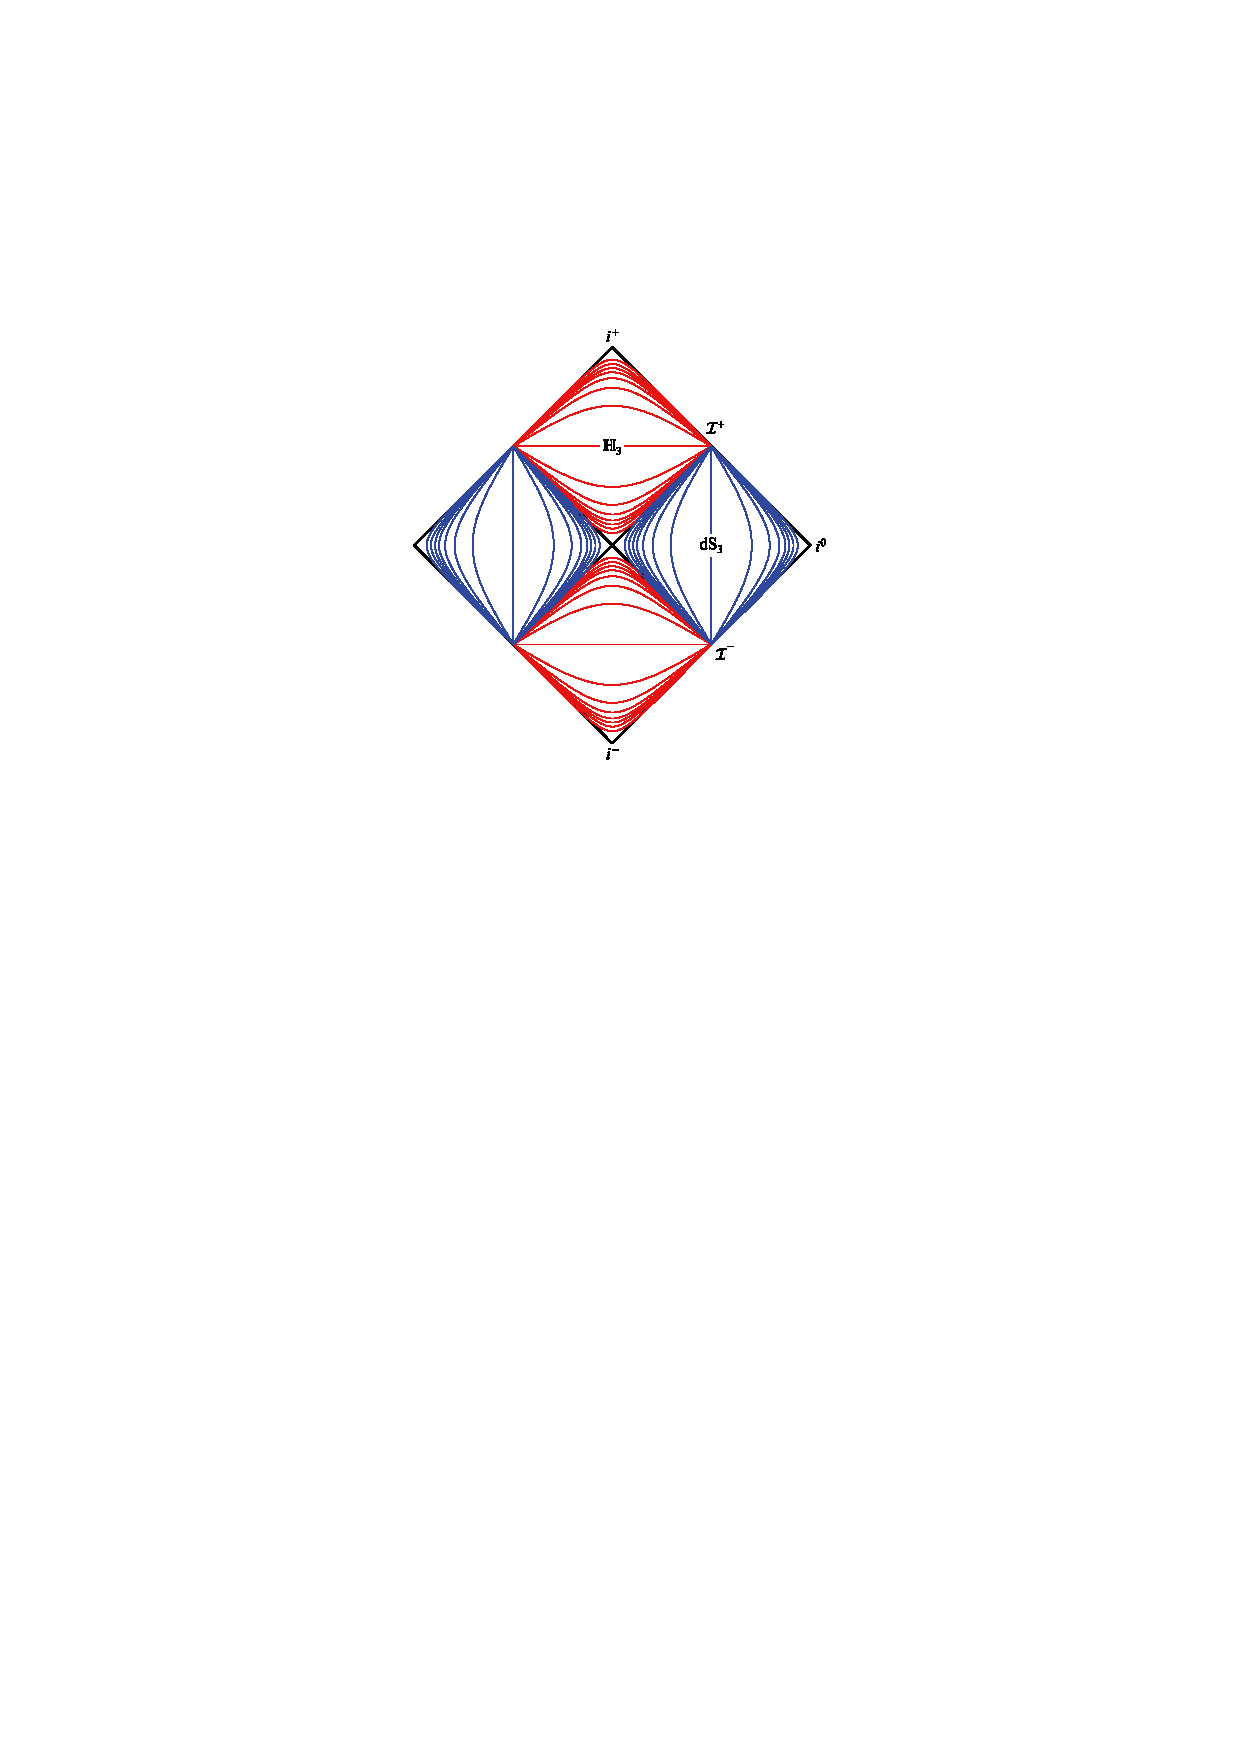
\includegraphics{figs/fig6.pdf}
	\caption{$Mink_4$时空的叶状结构}
\end{figure}
我们只使用unit的那一层。AdS/CFT对偶里面有一个bulk-to-boundary传播子,在前面的参数化下定义为\cite{Witten:1998qj}:
\begin{equation}
	\boxed{
	G_\Delta(\hat{p};\vec{w})=\left(\frac{y}{y^2+|\vec{z}-\vec{w}|^2}\right)^\Delta =G_\Delta(\hat{p};q)=\frac{1}{(-\hat{p}\cdot q)^\Delta}
	}
\end{equation}
这个传播子在共形变换$q\to q^\prime$,以及所诱导的Lorentz变换$\hat p\to\hat p^\prime$下变换性质为:
\begin{equation}
	G_\Delta(\hat{p'};q')=\left|\frac{\partial\vec{w}'}{\partial\vec{w}}\right|^{-\Delta/d}G_\Delta(\hat{p};q)
\end{equation}
最终的基底肯定是用平面波$\exp\left[\pm im\hat{p}\cdot X\right]$线性组合得到的,这里$+$表示out态,$-$表示in态。而且线性组合要对所有在壳动量构成的平面波求和,所以积分是在$\mathbb{H}_{d+1}$上进行的,积分测度是上面的不变测度:
\begin{equation}
	\int_{\mathbb{H}_{d+1}}[d\hat{p}]\equiv\int_0^\infty\frac{dy}{y^{d+1}}\int d^d\vec{z}=\int_{\hat p^2=-1}\frac{d^{d+1}\hat{p}^i}{\hat{p}^0}
\end{equation}
由于KG方程是一个线性方程,所以线性组合之后的结果都是KG方程的解\sn{只要线性组合的系数与$X$无关就好}。由于$G_\Delta$在共形变换下刚好出来我们需要的共形变换因子,而诱导的Lorentz变换本身不贵改变$\hat p \cdot X$和积分测度,所以下面的积分就是满足条件的conformal basis:
\begin{equation}\label{27}
	\boxed{
	\phi_\Delta^\pm(X^\mu;\vec{w})=\int_{\mathbb{H}_{d+1}}[d\hat{p}]G_\Delta(\hat{p};\vec{w})\exp\left[\pm im\hat{p}\cdot X\right]
	}
\end{equation}
注意$\Delta$和$\vec{w}$是用来标记基底的,与$m$无关。但是上面的式子只是形式上的定义,第一不便于计算,第二上式对于$m\in\mathbb{R}_+$是发散的,只有对于$m\in-i{\mathbb{R}_+}$才收敛,所以上式应当看作是先把$m$变成纯虚数积分,然后延拓到实轴。所以考虑直接去找满足条件的KG方程的解,设试探解为:
\begin{equation}
	\phi_\Delta(X^\mu;\vec{w})=\frac{f(X^2)}{(-q\cdot X)^\Delta}
\end{equation}
代入方程得到:
\begin{equation}
	0=4X^2f''(X^2)-2(2\Delta-d-2)f'(X^2)-m^2f(X^2)
\end{equation}
这是虚宗量Bessel方程,考虑$X\to\infty$收敛的解,解正比于第二类修正Bessel函数:
\[f(X^2)\propto\left(\sqrt{-X^2}\right)^{\Delta-\frac{d}{2}}K_{\Delta-\frac{d}{2}}\left(m\sqrt{X^2}\right)\]
前面的比例系数可以从积分表达式\ref{27}积分后最终对比得到:
\begin{equation}
	\phi_\Delta^\pm(X^\mu;\vec{w})=\frac{2^{\frac d2+1}\pi^{\frac d2}}{(im)^{\frac d2}}\frac{(\sqrt{-X^2})^{\Delta-\frac d2}}{(-q(\vec{w})\cdot X\mp i\epsilon)^\Delta}K_{\Delta-\frac d2}(m\sqrt{X^2})
\end{equation}
$\mathcal{A}\equiv\bra{\textbf{out}}\mathcal{S}\ket{\text{in}}$,那么在conformal基底下的散射振幅和原先动量空间散射振幅之间关系为:
\begin{equation}
	\widetilde{\mathcal{A}}(\Delta_i,\vec{w}_i)\equiv\prod_{k=1}^n\int_{\mathbb{H}_{d+1}}[d\hat{p}_k]G_{\Delta_k}(\hat{p}_k;\vec{w}_k)\mathcal{A}(\pm m_i\hat{p}_i^\mu)
\end{equation}
显然其具有CFT中n点关联函数性质:
\begin{equation}
	\widetilde{\mathcal A}(\Delta_{i},\vec{w}_{i}^{\prime}(\vec{w}_{i}))=\prod_{k=1}^{n}\left|\frac{\partial\vec{w}_{k}^{\prime}}{\partial\vec{w}_{k}}\right|^{-\Delta_{k}/d}\widetilde{\mathcal A}(\Delta_{i},\vec{w}_{i})
\end{equation}

前面一直在讲基底,但前面不对$\Delta$进行限制,构造出来的$\{\phi^{\pm}_{\Delta,\vec{w}}\}$极有可能是超完备的。下面我们要干的事情是在构造出来的这些基底里面选某一簇构造正交完备归一基底。

\begin{definition}[shadow transformation]
	对于一个共形维数为$\Delta$的(准)初级场$\mathcal{O}_\Delta(\vec{w})$,其\textbf{shadow}的定义为\cite{Ferrara:1972xe,Ferrara:1972ay,Ferrara:1972uq,Ferrara:1972kab}:
	\begin{equation}
		\begin{aligned}\widetilde{\mathcal{O}}_\Delta(\vec{w})&\equiv\frac{\Gamma(\Delta)}{\pi^{\frac{d}{2}}\Gamma(\Delta-\frac{d}{2})}\int d^d\vec{w}'\frac{1}{|\vec{w}-\vec{w}'|^{2(d-\Delta)}}\mathcal{O}_\Delta(\vec{w}')\end{aligned}
	\end{equation}
	不难发现,场的shadow变成了共形维数为$d-\Delta$的(准)初级场。
\end{definition}
由于$K_\alpha=K_{-\alpha}$,以及下面的恒等式\cite{Simmons-Duffin:2012juh}:
\begin{equation}
	\int d^{d}\vec{z}\frac{1}{|\vec{z}-\vec{w}|^{2(d-\Delta)}}\frac{1}{(-q(\vec{z})\cdot X)^{\Delta}}=\frac{\pi^{\frac{d}{2}}\Gamma(\Delta-\frac{d}{2})}{\Gamma(\Delta)}\frac{(-X^{2})^{\frac{d}{2}-\Delta}}{(-q(\vec{w})\cdot X)^{d-\Delta}}
\end{equation}
得到了一个核心等式:
\begin{equation}\label{eq:27.17}
	\boxed{\widetilde{\phi_\Delta^\pm}(X;\vec{w})=\phi_{d-\Delta}^\pm(X;\vec{w})}
\end{equation}
这实际上直接把空间一分为二,分成某个子空间和它的shadow,我们只用取其中一个构成基就好,因为它的shadow是其线性组合。

在考虑$SO(d+1,1)$的无限维表示\sn{\cite{Sun:2021rrs,Sun:2021thf}这两篇文章比较易读,而且重在比较新,文章\cite{Bissi:2023bhv}的$\S 2.2$是对此内容的一个简短review,更多的阅读材料可以在那里找到。}时会出现所谓\textbf{principal continuous series}的概念:
\begin{equation}
	\boxed{\Delta\in\frac d2+i\mathbb{R}}
\end{equation}
后面构造conformal basis就是用这一series里面的$\Delta$或其子集进行构造,这一点不加证明,后面只是去说明这样确实能得到正确的基底。

首先注意到关于$G_\Delta$的几个正交完备性关系\cite{Costa:2014kfa}:
\begin{equation}
	\int_{-\infty}^{\infty}d\nu\mu(\nu)\int d^{d}\vec{w}G_{\frac{d}{2}+i\nu}(\hat{p}_{1};\vec{w})G_{\frac{d}{2}-i\nu}(\hat{p}_{2};\vec{w})=\delta^{(d+1)}(\hat{p}_{1},\hat{p}_{2})
\end{equation}
这里$\delta$函数是定义在$\mathbb{H}_{d+1}$上也就是$SO(d+1,1)$不变的,积分测度$\mu(\nu)$:
\begin{equation}
	\mu(\nu)=\frac{\Gamma(\frac d2+i\nu)\Gamma(\frac d2-i\nu)}{4\pi^{d+1}\Gamma(i\nu)\Gamma(-i\nu)}
\end{equation}
还有一个
\begin{equation}
	\begin{gathered}
		\int_{H_{d+1}}[d\hat{p}]G_{\frac d2+i\nu}(\hat{p};\vec{w}_{1})G_{\frac d2+i\bar{\nu}}(\hat{p};\vec{w}_{2})= \\
		2\pi^{d+1}\frac{\Gamma(i\nu)\Gamma(-i\nu)}{\Gamma(\frac d2+i\nu)\Gamma(\frac d2-i\nu)}\delta(\nu+\bar{\nu})\delta^{(d)}(\vec{w}_{1}-\vec{w}_{2})+2\pi^{\frac d2+1}\frac{\Gamma(i\nu)}{\Gamma(\frac d2+i\nu)}\delta(\nu-\bar{\nu})\frac{1}{|\vec{w}_{1}-\vec{w}_{2}|^{2(\frac d2+i\nu)}}.
	\end{gathered}
\end{equation}
利用这些关系可以得到\ref{27}的逆变换:
\begin{equation}
	\boxed{e^{\pm im\hat{p}\cdot X}=2\int_0^\infty d\nu\mu(\nu)\int d^d\vec{w}G_{\frac d2-i\nu}(\hat{p};\vec{w})\phi_{\frac d2+i\nu}^\pm(X^\mu;\vec{w})}
\end{equation}
由于平面波基底完备,逆变换的存在性立刻就说明了利用principal continuous series构造出来的$\{\phi^{\pm}_{\Delta,\vec{w}}\}$也完备,而且注意到我们这里利用\ref{eq:27.17}将$\nu$限制在了$\mathbb{R}_+$上,所以:
\begin{equation}\label{eq:27.23}
	\boxed{\Delta\in\frac d2+i\mathbb{R}_{\geq 0}}
\end{equation}
这佐证了前面提到的只需要在空间和其shadow里面取一个就好了。正交性依赖于内积的定义,这里自然的定义KG内积:
\begin{equation}
	(\Phi_1,\Phi_2)=-i\int_\Sigma d^{d+1}X^i\left[\Phi_1(X)\partial_{X^0}\Phi_2^*(X)-\partial_{X^0}\Phi_1(X)\Phi_2^*(X)\right]
\end{equation}
这个定义是Poincar\'e不变的,是与Cauchy面选取无关的。计算得到:
\begin{equation}
	\begin{aligned}
		\left(\phi_{\frac{d}{2}+i\nu_{1}}^{\pm}(X^{\mu};\vec{w_{1}})\right.,&\left.\phi_{\frac{d}{2}+i\nu_{2}}^{\pm}(X^{\mu};\vec{w_{2}})\right) \\
		=&\pm\frac{2^{d+3}\pi^{2d+2}}{m^{d}}\frac{\Gamma(i\nu_{1})\Gamma(-i\nu_{1})}{\Gamma(\frac{d}{2}+i\nu_{1})\Gamma(\frac{d}{2}-i\nu_{1})}\delta(\nu_{1}-\nu_{2})\delta^{(d)}(\vec{w}_{1}-\vec{w}_{2}) \\
		&\pm\cancelto{0}{\frac{2^{d+3}\pi^{\frac{3d}{2}+2}}{m^{d}}\frac{\Gamma(i\nu_{1})}{\Gamma(\frac{d}{2}+i\nu_{1})}\delta(\nu_{1}+\nu_{2})\frac{1}{|\vec{w}_{1}-\vec{w}_{2}|^{2(\frac{d}{2}+i\nu_{1})}}}
	\end{aligned}
\end{equation}
第二项为$0$是因为\ref{eq:27.23}。总结一下,我们得到了$\ket{\text{in}}$和$\ket{\text{out}}$态的基底为:
\begin{equation}
	\boxed{\mathcal{B}^{\pm}=\left\{\begin{array}{c|c}\phi_{\frac{d}{2}+i\nu}^{\pm}(X;\vec{w})&\nu\geq0,\vec{w}\in\mathbb{R}^d\end{array}\right\}}
\end{equation}
它的shadow同样是一组基底:
\begin{equation}
	\boxed{\widetilde{\mathcal{B}}^\pm=\left\{\begin{array}{c|c}\phi_{\frac{d}{2}+i\nu}^\pm(X;\vec{w})&\nu\le0,\vec{w}\in\mathbb{R}^d\end{array}\right\}}
\end{equation}
\subsection{Massless Scalar}
无质量情况看作是有质量情况的极限,作换元$\omega\equiv\frac{m}{2y}$,积分核有如下渐近行为:
\begin{equation}
	G_{\Delta}(y,\vec{z};\vec{w})\xrightarrow{m\to0}\pi^{\frac{d}{2}}\frac{\Gamma(\Delta-\frac{d}{2})}{\Gamma(\Delta)}y^{d-\Delta}\delta^{(d)}(\vec{z}-\vec{w})+\frac{y^{\Delta}}{|\vec{z}-\vec{w}|^{2\Delta}}+\cdots 
\end{equation}
计算得到:
\begin{equation}
	\begin{aligned}\phi_{\frac{d}{2}+i\nu}^{\pm}(X;\vec{w})\xrightarrow{m\to0}&\left(\frac{m}{2}\right)^{-\frac{d}{2}-i\nu}\frac{\pi^{\frac{d}{2}}\Gamma(i\nu)}{\Gamma(\frac{d}{2}+i\nu)}\int_{0}^{\infty}d\omega\omega^{\frac{d}{2}+i\nu-1}e^{\pm i\omega q(\vec{w})\cdot X}\\+&\left(\frac{m}{2}\right)^{-\frac{d}{2}+i\nu}\int d^{d}\vec{z}\frac{1}{|\vec{z}-\vec{w}|^{2(\frac{d}{2}+i\nu)}}\int_{0}^{\infty}d\omega\omega^{\frac{d}{2}-i\nu-1}e^{\pm i\omega q(\vec{z})\cdot X}\end{aligned}
\end{equation}
上面的极限不是well-define的,因为$m^{\pm i\nu}$,但这是个相位,不妨先丢掉,而第二项是第一项的shadow,所以猜测最终应该是下面的形式:
\begin{equation}
	\boxed{\varphi_\Delta^\pm(X^\mu;\vec w)\equiv\int_0^\infty d\omega\omega^{\Delta-1}e^{\pm i\omega q\cdot X-\epsilon\omega}=\frac{(\mp i)^\Delta\Gamma(\Delta)}{(-q(\vec w)\cdot X\mp i\epsilon)^\Delta}}
\end{equation}
其中$\Delta\in\mathbb{C}$,需要重新去找寻。这个式子的形式就是所谓\textbf{Mellin变换}\sn{数学上Mellin变换定义为:\[\widetilde{f}(\Delta)=\int_0^\infty d\omega\omega^{\Delta-1}f(\omega)\]其逆变换为:\[f(\omega)=\frac1{2\pi i}\int_{c-i\infty}^{c+i\infty}d\Delta\omega^{-\Delta}\widetilde{f}(\Delta),c\in\mathbb{R}\]},可以解释成对未来光锥上的某一条射线积分,也就是把所有同“方向”,不同“能量”的平面波组合。注意这个式子有个非常明显的特征,在除去一个归一化因子的意义下,上式结果与$G_\Delta$将$q$替换为$X$得到的结果完全一致。上面变换的逆变换为:
\begin{equation}
	e^{\pm i\omega q\cdot X-\epsilon\omega}=\int_{-\infty}^{\infty}\frac{d\nu}{2\pi}\omega^{-\Delta}\frac{(\mp i)^{\Delta}\Gamma(
		\Delta)}{(-q\cdot X\mp i\epsilon)^{\Delta}},\quad\omega>0,\Re(\Delta)>0
\end{equation}
这说明了$\Re(\Delta)>0$就能保证完备性,而且这组基底张成的空间中很重要的一点是不含零动量的平面波解\sn{这一点是必须的,因为他是KG方程没有物理意义的解,要抛弃掉}。如果选取$\Re(\Delta)=\frac{d}{2}$,$\Im(\Delta)\in\mathbb{R}$,则:
\begin{equation}
	\begin{pmatrix}\varphi_{\frac{d}{2}+i\nu_{1}}^{\pm}(X^{\mu};\vec{w}_{1}),\varphi_{\frac{d}{2}+i\nu_{2}}^{\pm}(X^{\mu};\vec{w}_{2})\end{pmatrix}=\pm8\pi^{d+2}\delta(\nu_{1}-\nu_{2})\delta^{(d)}(\vec{w}_{1}-\vec{w}_{2})
\end{equation}
这个时候注意shadow:
\begin{equation}
	\begin{aligned}
		\widetilde{\varphi_{\frac{d}{2}+i\nu}^{\pm}}(X^{\mu};\vec{w})& =\frac{\Gamma(\frac{d}{2}+i\nu)}{\pi^{\frac{d}{2}}\Gamma(i\nu)}\int d^{d}\vec{z}\frac{1}{|\vec{z}-\vec{w}|^{2(\frac{d}{2}-i\nu)}}\varphi_{\frac{d}{2}+i\nu}^{\pm}(X^{\mu};\vec{z})  \\
		&=(\mp i)^{\frac d2+i\nu}\Gamma(\frac d2+i\nu)\frac{(-X^2)^{-i\nu}}{(-q(\vec{w})\cdot X\mp i\epsilon)^{\frac d2-i\nu}}\\
		\left(\varphi_{\frac{d}{2}+i\nu_1}^{\pm}(X^{\mu};\vec{w_1}),\right.&\left.\widetilde{\varphi_{\frac{d}{2}+i\nu_2}^{\pm}}(X^{\mu};\vec{w_2})\right)=\pm8\pi^{\frac{d}{2}+2}\frac{\Gamma(\frac{d}{2}-i\nu_1)}{\Gamma(-i\nu_1)}\delta(\nu_1-\nu_2)\frac{1}{|\vec{w_1}-\vec{w_2}|^{2(\frac{d}{2}+i\nu_1)}}
	\end{aligned}
\end{equation}
其shadow当然也是一组基底,但并不是$\nu\to-\nu$这么简单了,这导致$\nu$的取值范围也拓宽到了所有实数。总结一下,我们得到了Massless scalar的conformal basis:
\begin{equation}
	\boxed{\mathcal{B}_{m=0}^{\pm}=\left\{\begin{array}{c|c}\varphi_{\frac{d}{2}+i\nu}^{\pm}(X^{\mu};\vec{w})&\nu\in\mathbb{R},\vec{w}\in\mathbb{R}^{d}\end{array}\right\}}
\end{equation}
其shadow也可以作为一组基:
\begin{equation}
	\boxed{\widetilde{\mathcal{B}}_{m=0}^{\pm}=\left\{\begin{array}{c|c}\widetilde{\varphi_{\frac{d}{2}+i\nu}^{\pm}}(X^{\mu};\vec{w})&\nu\in\mathbb{R},\vec{w}\in\mathbb{R}^{d}\end{array}\right\}}
\end{equation}
\subsection{Phonton \& Graviton}
这两个除了自旋不为0,还有一个比较麻烦的点是需要取定规范。由于自旋不为0,所以基底除了在壳动量、初末态的$\pm$,以及极化矢量带来的$SO(1,d+1)$矢量指标,还需要一个指标用来标记自旋,这里考虑的是无质量玻色子,所以这个指标标记的是粒子的螺旋度,体现为CFT$_d$上的一个$\mathbb{R}^d$张量指标,$a=1,2,\ldots,d$。令在壳动量$k=\omega q$,在Loren规范下可以把平面波基底写为下面的形式:\sn{\[\partial_aq^\mu\equiv\frac{\partial}{\partial w^a}q^\mu(\vec{w})=2(w^a,\delta^{ba},-w^a)\]}:
\begin{equation}
	\partial_aq_\mu e^{\pm i\omega q\cdot X}
\end{equation}
注意Lorenz规范只能将前面的极化矢量确定到一个正比于$k$的项,选取这样的形式相当于完全取定了规范。不难验证$d=2$时,上面的选取就对应\ref{eq:24.7}的选取。
\begin{definition}[Spin\mbox{-}1 Massless Boson, $d\geq 1$]
	~
	\begin{itemize}
		\item 在壳:\footnote{满足的是Proca方程}
		\begin{equation}
			\left(\frac{\partial}{\partial X^\sigma}\frac{\partial}{\partial X_\sigma}\delta_\nu^\mu-\frac{\partial}{\partial X^\nu}\frac{\partial}{\partial X_\mu}\right)A_{\mu a}^{\Delta\pm}(X^\rho;\vec{w})=0
		\end{equation}
		\item 协变:
		\begin{equation}
			A_{\mu a}^{\Delta\pm}\left(\Lambda^{\rho}{}_{\nu}X^{\nu};\vec{w}'(\vec{w})\right)=\frac{\partial w^{b}}{\partial{w'^{a}}}\left|\frac{\partial\vec{w}'}{\partial\vec{w}}\right|^{-(\Delta-1)/d}\Lambda_{\mu}{}^{\sigma}A_{\sigma b}^{\Delta\pm}(X^{\rho};\vec{w})
		\end{equation}
	\end{itemize}
\end{definition}
$\mathbb{H}_{d+1}$上面的 Spin\mbox{-}1 bulk-to boundary 传播子为$G^\Delta_{\mu;q}$\sn{后面只要是$a,b,c$指标就是$\mathbb{R}^d$上的,在只要是$\mu,\nu,\sigma$指标就是$\mathbb{R}^{1,d+1}$上的},计算上更常用的是其 \textbf{uplift} $G^\Delta_{\mu;\nu}$,定义为:\sn{其实就是拉回映射}
\begin{equation}
	G^\Delta_{\mu;q}=\frac{\partial q^\nu}{\partial w^a}G_{\mu;\nu}^\Delta(\hat{p};q)
\end{equation}
\begin{equation}
	G_{\mu;\nu}^{\Delta}(\hat{p};q)=\frac{(-q\cdot\hat{p})\eta_{\mu\nu}+q_{\mu}\hat{p}_{\nu}}{(-q\cdot\hat{p})^{\Delta+1}}
\end{equation}
uplift之后,$G^\Delta_{\mu;\nu}$就是一个标量CFT$_d$,而且是$\mathbb{R}^{1,d+1}$上的2\mbox{-}tensor:
\begin{equation}
	G_{\mu;\nu}^{\Delta}(\Lambda\hat{p};\Lambda q)=\left|\frac{\partial\vec{w}'}{\partial\vec{w}}\right|^{-\Delta/d}\Lambda^{\rho}{}_{\mu}\Lambda^{\sigma}{}_{\nu}G^{\Delta}{}_{\rho;\sigma}(\hat{p};q)
\end{equation}
而且关于两个自变量还满足横向条件:
\begin{equation}\label{eq:t}
	\hat{p}^{\mu}G_{\mu;\nu}^{\Delta}(\hat{p};q)=0,\quad q^{\nu}G_{\mu;\nu}^{\Delta}(\hat{p};q)=0
\end{equation}
根据前面的标量场经验,不难猜测$A$的形式就是$G$把$q$换成$X$:
\begin{equation}
	\boxed{
		\begin{aligned}
			A_{\mu a}^{\Delta,\pm}(X^{\mu};\vec{w})& {=\frac{\partial_{a}q_{\mu}}{(-q\cdot X\mp i\epsilon)^{\Delta}}+\frac{\partial_{a}q\cdot X}{(-q\cdot X\mp i\epsilon)^{\Delta+1}}q_{\mu}} \\
			&=-\frac{1}{(-q\cdot X\mp i\epsilon)^{\Delta-1}}\frac{\partial}{\partial X^{\mu}}\frac{\partial}{\partial w^{a}}\log(-q\cdot X\mp i\epsilon)
		\end{aligned}
	}
\end{equation}
证明略。下面计算其shadow。
\begin{definition}[shadow for spinning fields]
	对于自旋为$J$的场,其会导致带有$J$个$\mathbb{R}^d$上的指标$a_1,\ldots,a_J$,而且这些指标是无迹且全对称的,或者说$\mathcal{O}^\Delta_{a_1\cdot\cdot\cdot a_J}(\vec{w})$是$SO(d)$的无迹对称张量表示,即Spin\mbox{-}J表示。计算其shadow最简单的方式是使用其uplift计算,然后再投影回来,uplift与其自身的关系为:
	\begin{equation}
		\mathcal{O}^\Delta_{a_1\cdots a_J}(\vec{w})=\frac{\partial q^{\mu_1}}{\partial w^{a_1}}\cdots\frac{\partial q^{\mu_J}}{\partial w^{a_J}}\mathcal{O}^\Delta_{\mu_1\cdots\mu_J}(\vec{w})
	\end{equation}
	uplift与其自变量之间存在类似\ref{eq:t}的横向关系。
	\begin{equation}
		\boxed{
		\widetilde{\mathcal{O}^\Delta}_{\mu_1\cdots\mu_J}(\vec{w})=\frac{\Gamma(\Delta+J)}{\pi^{\frac d2}(\Delta-1)_J\Gamma(\Delta-\frac d2)}\int d^d\vec{w}^{\prime}\frac{\prod_{n=1}^J\left[\delta_{\mu_n}^{\nu_n}(-\frac12q\cdot q^{\prime})+\frac12q_{\mu_n}^{\prime}q^{\nu_n}\right]}{(-\frac12q\cdot q^{\prime})^{d-\Delta+J}}\mathcal{O}^\Delta_{\nu_1\cdots\nu_J}(\vec{w}^{\prime})}
	\end{equation}
	这里$(a)_{J}\equiv\Gamma(a+J)/\Gamma(a)$,称为Pochhammer符号,而且不难发现上面的定义对于某些$\Delta$不是well-define的,所以需要解析延拓到全部复平面。
\end{definition}
利用上面定义计算得到:
\begin{equation}
	\boxed{
	\widetilde{A_{\mu a}^{\Delta,\pm}}(X^\mu;\vec{w})=(-X^2)^{\frac{d}{2}-\Delta}A_{\mu a}^{d-\Delta,\pm}(X^\mu;\vec{w})
	}
\end{equation}
和无质量标量场一样,不是正比于$A_{\mu a}^{d-\Delta,\pm}$。现在还没有讨论我们的计算是在哪个规范下进行的,但其实前面对$A_{\mu a}^{\Delta,\pm}$那些在壳协变的要求就已经为我们完全取定了规范,是Lorenz和radial规范同时加上去:\sn{这两个规范是可以同时取的,见\cite{PhysRevD.76.084013}}
\begin{equation}
	X^{\mu}A_{\mu a}^{\Delta,\pm}(X^{\mu};\vec{w})=0,\quad\partial^{\mu}A_{\mu a}^{\Delta,\pm}(X^{\mu};\vec{w})=0.
\end{equation}
下表总结了$A_{\mu a}^{\Delta,\pm}$及其 shadow 为 pure gauge\sn{pure gauge就是说可以从$A=0$通过规范变换变过来,所以场强张量为0,$A$可以写为$\frac{i}{g}U\partial_\mu U^\dagger$的形式}的条件:
\begin{center}
	\begin{tabular}[H]{|c|c|c|}
		\hline & $d=2$ & $d \neq 2$ \\
		\hline$A_{\mu a}^{\Delta, \pm}$ & & $\Delta=1$ \\
		& $\Delta=1$ & \\
		$\widetilde{A_{\mu a}^{d-\Delta, \pm}}$& & $\times$ \\
		\hline
	\end{tabular}
\end{center}
回顾一些前面给的平面波基底是在Lorenz规范下给的,不一定满足radial规范,所以$A$不能写成平面波基底的积分变换形式,但是:
\begin{equation}
	\boxed{
	\varphi_{\mu a}^{\Delta,\pm}(X^{\mu};\vec{w})=\int_0^\infty d\omega\omega^{\Delta-1}\left(\partial_aq_\mu e^{\pm i\omega q\cdot X-\epsilon\omega}\right)=(\mp i)^\Delta\Gamma(\Delta)\frac{\partial_aq_\mu}{(-q\cdot X\mp i\epsilon)^\Delta}
	}
\end{equation}
和$A_{\mu a}^{\Delta,\pm}$之间只差一个规范变换\sn{$\frac{\partial}{\partial X^\mu}\left(\frac{\partial_aq\cdot X}{(-q\cdot X\mp i\epsilon)^\Delta}\right)$},那么在计算散射振幅这种与规范选取无关的物理量的时候,用两组基底都能得到同样的结果,但是注意用$\varphi_{\mu a}^{\Delta,\pm}$做基底的时候就没有协变的条件了,但是好处在两基底振幅之间是Mellin变换的形式。在下面的内积定义下:
\begin{equation}
	(A_{\mu},A'_{\mu'})=-i\int _\Sigma d^{d+1}X^i\left[A^{\rho}F'^*_{0\rho}-A'^{\rho*}F_{0\rho}\right]
\end{equation}
当选取$\boxed{\Delta\in\frac{d}{2}+\mathrm{i}\mathbb{R}}$时构成完备基底,其shadow亦然。

这组基底虽说是Phonton的,但实际上非阿贝尔情形也完全适用,因为每个色指标的场满足相同的方程,相同的协变条件,所以上面的推导完全不变,这是很容易接受的,因为平面波基底对于phonton和gluon都是一样通用的。

现在来看引力子的情况,首先在Lorenz\sn{$\partial^{\mu}h_{\mu\nu}-\frac12\partial_{\nu}h^{\rho}{}_{\rho}=0,$}、无迹规范下平面波基底可以写为:
\begin{equation}
	g_{\mu\nu;a_1a_2}^{\pm}(X;\omega,q)=P_{a_1a_2}^{b_1b_2}\partial_{b_1}q_\mu\partial_{b_2}q_\nu e^{\pm i\omega q\cdot X}
\end{equation}
这里:
\begin{equation}
	P_{a_1a_2}^{b_1b_2}\equiv\delta_{(a_1}^{b_1}\delta_{a_2)}^{b_2}-\frac{1}{d}\delta_{a_1a_2}\delta^{b_1b_2}
\end{equation}
\begin{definition}[Graviton, $d\geq 2$]
	~
	\begin{itemize}
		\item 指标约束:
		\begin{equation}
			\begin{array}{l}h_{\mu_1\mu_2;a_1a_2}^{\Delta,\pm}=h_{\mu_2\mu_1;a_1a_2}^{\Delta,\pm},\\h_{\mu_1\mu_2;a_1a_2}^{\Delta,\pm}=h_{\mu_1\mu_2;a_2a_1}^{\Delta,\pm},\quad\delta^{a_1a_2}h_{\mu_1\mu_2;a_1a_2}^{\Delta,\pm}=0\end{array}
		\end{equation}
		第一个约束是几何上要求度规对称,第二个是要求$\mathbb{R}^d$指标无迹且对称。
		\item 在壳:\footnote{满足的是Linearized Einstein方程}
		\begin{equation}
			\partial_\sigma\partial_\nu {h^\sigma}_{\mu;a_1a_2}+\partial_\sigma\partial_\mu {h^\sigma}_{\nu;a_1a_2}-\partial_\mu\partial_\nu {h^\sigma}_{\sigma;a_1a_2}-\partial^\rho\partial_\rho h_{\mu\nu;a_1a_2}=0
		\end{equation}
		\item 协变:
		\begin{equation}
			h_{\mu_1\mu_2;a_1a_2}^{\Delta,\pm}\left(\Lambda_{\nu}^{\rho}X^{\nu};\vec{w}'(\vec{w})\right)=\frac{\partial w^{b_1}}{\partial w'^{a_1}}\frac{\partial w^{b_2}}{\partial w'^{a_2}}\left|\frac{\partial\vec{w'}}{\partial\vec{w}}\right|^{-(\Delta-2)/d}\Lambda_{\mu_1}^{\sigma_1}\Lambda_{\mu_2}^{\sigma_2}h_{\sigma_1\sigma_2;b_1b_2}^{\Delta,\pm}(X^\rho;\vec{w})
		\end{equation}
	\end{itemize}
\end{definition}
利用$\mathbb{H}_{d+1}$上面的 Spin\mbox{-}2 bulk-to boundary 传播子:
\begin{equation}\label{eq:27.55}
	\boxed{
		\begin{aligned}
			h_{\mu_1\mu_2;a_1a_2}^{\Delta,\pm}(X;\vec{w})&=P_{a_1a_2}^{b_1b_2}\frac{\left[(-q\cdot X)\partial_{b_1}q_{\mu_1}+(\partial_{b_1}q\cdot X)q_{\mu_1}\right]\left[(-q\cdot X)\partial_{b_2}q_{\mu_2}+(\partial_{b_2}q\cdot X)q_{\mu_2}\right]}{(-q\cdot X)^{\Delta+2}}\\
			&=P_{a_{1}a_{2}}^{b_{1}b_{2}}\frac{1}{(-q\cdot X\mp i\epsilon)^{\Delta-2}}\partial_{b_{1}}\partial_{\mu_{1}}\log(-q\cdot X\mp i\epsilon)\partial_{b_{2}}\partial_{\mu_{2}}\log(-q\cdot X\mp i\epsilon)
		\end{aligned}
		}
\end{equation}
其shadow:
\begin{equation}
	\widetilde {h_{\mu_1\mu_2;a_1a_2}^{\Delta,\pm}}(X;\vec{w})=(-X^2)^{\frac{d}{2}-\Delta}h_{\mu_1\mu_2;a_1a_2}^{d-\Delta,\pm}(X;\vec{w})
\end{equation}
前面实际上选取了规范:
\begin{equation}
	\eta^{\mu_1\mu_2}h_{\mu_1\mu_2;a_1a_2}^{\Delta,\pm}=0,\quad\partial^{\mu}h_{\mu\mu_2;a_1a_2}^{\Delta,\pm}=0,\quad X^{\mu}h_{\mu\mu_2;a_1a_2}^{\Delta,\pm}=0
\end{equation}
有Pure gauge条件:\sn{可以写为$\partial_{(\mu}\xi_{\nu)}$的形式}
\begin{center}
	\begin{tabular}[H]{|c|cc|c|}
		\hline & \multicolumn{2}{c|}{$d=2$} & $d \geq 2$ \\
		\hline$h_{\mu_1\mu_2;a_1a_2}^{\Delta,\pm}$ & &$\Delta=0$& $\Delta=0,1$ \\
		& $\Delta=1$ & & \\
		$\widetilde{h_{\mu_1\mu_2;a_1a_2}^{d-\Delta,\pm}}$& &$\Delta=2$ & $\times$ \\
		\hline
	\end{tabular}
\end{center}
同样,前面的平面波基底不满足radial规范,但利用Mellin变换后得到的:
\begin{equation}
	\boxed{
	\begin{aligned}
		\varphi_{\mu_1\mu_2;a_1a_2}^{\Delta,\pm}(X^\mu;\vec{w})&=\int_0^\infty d\omega\omega^{\Delta-1}g_{\mu_1\mu_2;a_1a_2}^{\Delta,\pm}(X^\mu;\omega,q^\mu)\\&=(\mp i)^\Delta\Gamma(\Delta)P_{a_1a_2}^{b_1b_2}\frac{\partial_{b_1}q_{\mu_1}\partial_{b_2}q_{\mu_2}}{(-q\cdot X\mp i\epsilon)^\Delta}
	\end{aligned}
}
\end{equation}
与\ref{eq:27.55}只差一个规范变换\begin{margintable}\footnotesize 
	\begin{tabularx}{\marginparwidth}{|X}
		Because:
		\[\frac{\partial_bq_{(\mu_1}q_{\mu_2)}}{(-q\cdot X)^\Delta}=\frac{\partial_{(\mu_1}}{\Delta-1}\left(\frac{\partial_bq_{\mu_2)}}{(-q\cdot X)^{\Delta-1}}\right)\]
		\[\frac{q_{\mu_1}q_{\mu_2}}{(-q\cdot X)^\Delta}=\frac{\partial_{(\mu_1}}{\Delta-1}\left(\frac{q_{\mu_2)}}{(-q\cdot X)^{\Delta-1}}\right)\]
	\end{tabularx}
\end{margintable}。在下面的内积意义下:
\begin{equation}
	\begin{aligned}
		(h_{\mu\nu},h_{\mu^{\prime}\nu^{\prime}}^{\prime})& =-i\int d^{d+1}X^{i}\Big[h^{\mu\nu}\partial_{0}{h^{\prime}}_{\mu\nu}^{*}-2h^{\mu\nu}\partial_{\mu}{h^{\prime}}_{0\nu}^{*}+h\partial^{\mu}{h^{\prime}}_{0\mu}^{*}-h\partial_{0}{h^{\prime}}^{*}+h_{0\mu}{\partial^{\mu}{h^{\prime}}^{*}}  \\
		&-(h\leftrightarrow{h^{\prime}}^{*})\Big]
	\end{aligned}
\end{equation}
$\boxed{\Delta\in\frac{d}{2}+\mathrm{i}\mathbb{R}}$时构成完备基底,其shadow亦然。
\begin{remark}
	$SO(1,d+1)$群的无限维不可约幺正表示由共形维数$\Delta\in\mathbb{C}$和$SO(d)$的表示去标记(或者说取决于对应的$SO(d)$是哪个自旋表示)。前面找的基底就是在找表示,$\Delta$和$J$之间是有约束的,具体来说有下面几个Series:
	\begin{itemize}
		\item Principal Series $\mathcal{P}$: $\forall J\in\mathbb{N},\quad \Delta\in\frac{d}{2}+\mathrm{i}\mathbb{R}$
		\item Complementary Series $\mathcal{C}$: $\Delta=\frac{d}{2}+c$,其中$J=0$时$0<|c|\leq\frac{d}{2}$,$J\geq 1$时$0<|c|\leq\frac{d}{2}-1$
		\item Discrete Series $\mathcal{D}$: 对于奇数维数$d$,任意$J$,$\Delta$可取半整数或者整数
	\end{itemize}
	表示$[\Delta,J]$的shadow就是表示$[d-\Delta,J]$,这两个表示是等价表示。
\end{remark}
\newpage
\subsection{Restrict to Mink$_{4}$}
根据前面的一系列一般性讨论,回到Mink$_{4}$情况很简单,这里只是用文献中比较常用的记号重新写一遍。\sn{\cite{Donnay:2020guq}$\S 2$基本上是很好的总结}

标量场:
\begin{equation}
	\phi_{\Delta,m}\left(\Lambda^{\mu}{}_{\nu}X^{\nu};\frac{aw+b}{cw+d},\frac{\bar{a}\bar{w}+\bar{b}}{\bar{c}\bar{w}+\bar{d}}\right)=|cw+d|^{2\Delta}\phi_{\Delta,m}(X^{\mu};w,\bar{w})
\end{equation}

无质量规范玻色子:
\begin{equation}
	A_{\mu;a}^{\Delta,\pm}\left({\Lambda^{\rho}}_{\nu}X^{\nu};\frac{aw+b}{cw+d},\frac{\bar{a}\bar{w}+\bar{b}}{\bar{c}\bar{w}+\bar{d}}\right)=(cw+d)^{2h}(\bar{c}\bar{w}+\bar{d})^{2\bar{h}}{\Lambda_{\mu}}^{\sigma}A_{\sigma;a}^{\Delta,\pm}(X^{\rho};w,\bar{w})
\end{equation}
无质量规范玻色子只有两种螺旋度选取,对应这里$a=w,\bar w$,分别有$J=+1,-1$。

引力子:
\begin{equation}
	h_{\mu\nu;a}^{\Delta,\pm}\left(\Lambda^{\mu}{}_{\nu}X^{\nu};\frac{aw+b}{cw+d},\frac{\bar{a}\bar{w}+\bar{b}}{\bar{c}\bar{w}+\bar{d}}\right)=(cw+d)^{\Delta+J}(\bar{c}\bar{w}+\bar{d})^{\Delta-J}{\Lambda_{\mu}}^{\rho}{\Lambda_{\nu}}^{\sigma}h_{\rho\sigma,a}^{\Delta,\pm}(X^{\mu};w,\bar{w})
\end{equation}
同样的引力子也只有两种螺旋度选取,对应$a=ww,\bar w\bar w$,分别对应$J=+2,-2$。
不难看出这些情况共形权$(h,\bar h)=\frac12(\Delta+J,\Delta-J)$,$h-\bar h$确实就对应自旋。

\subsection{Conformally Soft phonton \& Graviton}
\subsection{Massive Bosons}
\subsection{Fermions}
\subsection{Examples}
	%\part{Appendix: Surface Charge}
% 计数器清零,每个part都要引用,除了part1
% 之后的每一个section这些次级目录都用带星号不编号的,整体的格式会和前面有比较大的差距
\part*{Appendix A: Surface Charge}{\marginnote{
		\begin{tcolorbox}[width=\marginparwidth,height=\marginparwidth/2,colback=black!50!white,colframe=black!50!white,center title,fonttitle=\bfseries\normalsize,title=APPENDIX,text fill]
			\begin{center}
				{\color{white} \Huge{A}}
			\end{center}
		\end{tcolorbox}
	}[-1.25in]}
\setcounter{theorem}{0}
\setcounter{definition}{0}
\setcounter{lemma}{0}
\setcounter{sidenote}{1}
前面介绍协变相空间量子化的时候直接使用结论,没有讲清楚他是什么,这里补上。
\section*{Fiber Bundle}
{\color{red}\hrule}
\hspace*{\fill} \\%手动添加分割线

to be continue \ldots
	
%	\begin{thebibliography}{99}
%	
%	\end{thebibliography}
	\nocite{*}
	\addcontentsline{toc}{part}{参考文献}
	\bibliographystyle{JHEP}
	\bibliography{ref.bib}
\end{document}